\documentclass[twoside]{book}

% Packages required by doxygen
\usepackage{fixltx2e}
\usepackage{calc}
\usepackage{doxygen}
\usepackage[export]{adjustbox} % also loads graphicx
\usepackage{graphicx}
\usepackage[utf8]{inputenc}
\usepackage{makeidx}
\usepackage{multicol}
\usepackage{multirow}
\PassOptionsToPackage{warn}{textcomp}
\usepackage{textcomp}
\usepackage[nointegrals]{wasysym}
\usepackage[table]{xcolor}

% Font selection
\usepackage[T1]{fontenc}
\usepackage[scaled=.90]{helvet}
\usepackage{courier}
\usepackage{amssymb}
\usepackage{sectsty}
\renewcommand{\familydefault}{\sfdefault}
\allsectionsfont{%
  \fontseries{bc}\selectfont%
  \color{darkgray}%
}
\renewcommand{\DoxyLabelFont}{%
  \fontseries{bc}\selectfont%
  \color{darkgray}%
}
\newcommand{\+}{\discretionary{\mbox{\scriptsize$\hookleftarrow$}}{}{}}

% Page & text layout
\usepackage{geometry}
\geometry{%
  a4paper,%
  top=2.5cm,%
  bottom=2.5cm,%
  left=2.5cm,%
  right=2.5cm%
}
\tolerance=750
\hfuzz=15pt
\hbadness=750
\setlength{\emergencystretch}{15pt}
\setlength{\parindent}{0cm}
\setlength{\parskip}{3ex plus 2ex minus 2ex}
\makeatletter
\renewcommand{\paragraph}{%
  \@startsection{paragraph}{4}{0ex}{-1.0ex}{1.0ex}{%
    \normalfont\normalsize\bfseries\SS@parafont%
  }%
}
\renewcommand{\subparagraph}{%
  \@startsection{subparagraph}{5}{0ex}{-1.0ex}{1.0ex}{%
    \normalfont\normalsize\bfseries\SS@subparafont%
  }%
}
\makeatother

% Headers & footers
\usepackage{fancyhdr}
\pagestyle{fancyplain}
\fancyhead[LE]{\fancyplain{}{\bfseries\thepage}}
\fancyhead[CE]{\fancyplain{}{}}
\fancyhead[RE]{\fancyplain{}{\bfseries\leftmark}}
\fancyhead[LO]{\fancyplain{}{\bfseries\rightmark}}
\fancyhead[CO]{\fancyplain{}{}}
\fancyhead[RO]{\fancyplain{}{\bfseries\thepage}}
\fancyfoot[LE]{\fancyplain{}{}}
\fancyfoot[CE]{\fancyplain{}{}}
\fancyfoot[RE]{\fancyplain{}{\bfseries\scriptsize Generated by Doxygen }}
\fancyfoot[LO]{\fancyplain{}{\bfseries\scriptsize Generated by Doxygen }}
\fancyfoot[CO]{\fancyplain{}{}}
\fancyfoot[RO]{\fancyplain{}{}}
\renewcommand{\footrulewidth}{0.4pt}
\renewcommand{\chaptermark}[1]{%
  \markboth{#1}{}%
}
\renewcommand{\sectionmark}[1]{%
  \markright{\thesection\ #1}%
}

% Indices & bibliography
\usepackage{natbib}
\usepackage[titles]{tocloft}
\setcounter{tocdepth}{3}
\setcounter{secnumdepth}{5}
\makeindex

% Hyperlinks (required, but should be loaded last)
\usepackage{ifpdf}
\ifpdf
  \usepackage[pdftex,pagebackref=true]{hyperref}
\else
  \usepackage[ps2pdf,pagebackref=true]{hyperref}
\fi
\hypersetup{%
  colorlinks=true,%
  linkcolor=blue,%
  citecolor=blue,%
  unicode%
}

% Custom commands
\newcommand{\clearemptydoublepage}{%
  \newpage{\pagestyle{empty}\cleardoublepage}%
}

\usepackage{caption}
\captionsetup{labelsep=space,justification=centering,font={bf},singlelinecheck=off,skip=4pt,position=top}

%===== C O N T E N T S =====

\begin{document}

% Titlepage & ToC
\hypersetup{pageanchor=false,
             bookmarksnumbered=true,
             pdfencoding=unicode
            }
\pagenumbering{alph}
\begin{titlepage}
\vspace*{7cm}
\begin{center}%
{\Large Vex Team A }\\
\vspace*{1cm}
{\large Generated by Doxygen 1.8.13}\\
\end{center}
\end{titlepage}
\clearemptydoublepage
\pagenumbering{roman}
\tableofcontents
\clearemptydoublepage
\pagenumbering{arabic}
\hypersetup{pageanchor=true}

%--- Begin generated contents ---
\chapter{In\+The\+ZoneA}
\label{md__r_e_a_d_m_e}
\Hypertarget{md__r_e_a_d_m_e}
Team A code for In The Zone 
\chapter{Data Structure Index}
\section{Data Structures}
Here are the data structures with brief descriptions\+:\begin{DoxyCompactList}
\item\contentsline{section}{\hyperlink{structlcd__buttons}{lcd\+\_\+buttons} \\*Repreents the state of the lcd buttons }{\pageref{structlcd__buttons}}{}
\item\contentsline{section}{\hyperlink{structmenu}{menu} }{\pageref{structmenu}}{}
\item\contentsline{section}{\hyperlink{structmenu__result}{menu\+\_\+result} }{\pageref{structmenu__result}}{}
\item\contentsline{section}{\hyperlink{structpolar__cord}{polar\+\_\+cord} \\*A struct that contains polar cordinates }{\pageref{structpolar__cord}}{}
\end{DoxyCompactList}

\chapter{File Index}
\section{File List}
Here is a list of all files with brief descriptions\+:\begin{DoxyCompactList}
\item\contentsline{section}{include/\hyperlink{battery_8h}{battery.\+h} }{\pageref{battery_8h}}{}
\item\contentsline{section}{include/\hyperlink{controller_8h}{controller.\+h} \\*Controller definitions, macros }{\pageref{controller_8h}}{}
\item\contentsline{section}{include/\hyperlink{drive_8h}{drive.\+h} \\*Drive base definitions and enumerations }{\pageref{drive_8h}}{}
\item\contentsline{section}{include/\hyperlink{encoders_8h}{encoders.\+h} \\*Wrapper around encoder functions }{\pageref{encoders_8h}}{}
\item\contentsline{section}{include/\hyperlink{lcd_8h}{lcd.\+h} \\*L\+CD wrapper functions and macros }{\pageref{lcd_8h}}{}
\item\contentsline{section}{include/\hyperlink{log_8h}{log.\+h} \\*Contains logging functions }{\pageref{log_8h}}{}
\item\contentsline{section}{include/\hyperlink{main_8h}{main.\+h} \\*Header file for global functions }{\pageref{main_8h}}{}
\item\contentsline{section}{include/\hyperlink{menu_8h}{menu.\+h} \\*Contains menu functionality and abstraction }{\pageref{menu_8h}}{}
\item\contentsline{section}{include/\hyperlink{ports_8h}{ports.\+h} \\*Port macros for sensors }{\pageref{ports_8h}}{}
\item\contentsline{section}{include/\hyperlink{slew_8h}{slew.\+h} \\*Contains the slew rate controller wrapper for the motors }{\pageref{slew_8h}}{}
\item\contentsline{section}{include/\hyperlink{vlib_8h}{vlib.\+h} \\*Contains misc helpful functions }{\pageref{vlib_8h}}{}
\item\contentsline{section}{include/\hyperlink{vmath_8h}{vmath.\+h} \\*Vex Specific Math Functions, includes\+: Cartesian to polar cordinates }{\pageref{vmath_8h}}{}
\item\contentsline{section}{src/\hyperlink{auto_8c}{auto.\+c} \\*File for autonomous code }{\pageref{auto_8c}}{}
\item\contentsline{section}{src/\hyperlink{battery_8c}{battery.\+c} }{\pageref{battery_8c}}{}
\item\contentsline{section}{src/\hyperlink{controller_8c}{controller.\+c} }{\pageref{controller_8c}}{}
\item\contentsline{section}{src/\hyperlink{drive_8c}{drive.\+c} }{\pageref{drive_8c}}{}
\item\contentsline{section}{src/\hyperlink{encoders_8c}{encoders.\+c} }{\pageref{encoders_8c}}{}
\item\contentsline{section}{src/\hyperlink{init_8c}{init.\+c} \\*File for initialization code }{\pageref{init_8c}}{}
\item\contentsline{section}{src/\hyperlink{lcd_8c}{lcd.\+c} }{\pageref{lcd_8c}}{}
\item\contentsline{section}{src/\hyperlink{log_8c}{log.\+c} }{\pageref{log_8c}}{}
\item\contentsline{section}{src/\hyperlink{menu_8c}{menu.\+c} }{\pageref{menu_8c}}{}
\item\contentsline{section}{src/\hyperlink{opcontrol_8c}{opcontrol.\+c} \\*File for operator control code }{\pageref{opcontrol_8c}}{}
\item\contentsline{section}{src/\hyperlink{slew_8c}{slew.\+c} }{\pageref{slew_8c}}{}
\item\contentsline{section}{src/\hyperlink{vlib_8c}{vlib.\+c} }{\pageref{vlib_8c}}{}
\item\contentsline{section}{src/\hyperlink{vmath_8c}{vmath.\+c} }{\pageref{vmath_8c}}{}
\end{DoxyCompactList}

\chapter{Data Structure Documentation}
\section{lcd\+\_\+buttons Struct Reference}
\label{structlcd__buttons}\index{lcd\+\_\+buttons@{lcd\+\_\+buttons}}


represents the state of the lcd buttons  




{\ttfamily \#include $<$lcd.\+h$>$}

\subsection*{Data Fields}
\begin{DoxyCompactItemize}
\item 
\textbf{ button\+\_\+state} \textbf{ left}
\item 
\textbf{ button\+\_\+state} \textbf{ middle}
\item 
\textbf{ button\+\_\+state} \textbf{ right}
\end{DoxyCompactItemize}


\subsection{Detailed Description}
represents the state of the lcd buttons 

\begin{DoxyAuthor}{Author}
Chris Jerrett 
\end{DoxyAuthor}
\begin{DoxyDate}{Date}
9/9/2017 
\end{DoxyDate}


Definition at line \textbf{ 48} of file \textbf{ lcd.\+h}.



\subsection{Field Documentation}
\mbox{\label{structlcd__buttons_ae385efb5ec794acf5f11027f46c6c039}} 
\index{lcd\+\_\+buttons@{lcd\+\_\+buttons}!left@{left}}
\index{left@{left}!lcd\+\_\+buttons@{lcd\+\_\+buttons}}
\subsubsection{left}
{\footnotesize\ttfamily \textbf{ button\+\_\+state} lcd\+\_\+buttons\+::left}



Definition at line \textbf{ 49} of file \textbf{ lcd.\+h}.



Referenced by \textbf{ lcd\+\_\+get\+\_\+pressed\+\_\+buttons()}.

\mbox{\label{structlcd__buttons_a293342810ac56f73979b08f144d6e6b9}} 
\index{lcd\+\_\+buttons@{lcd\+\_\+buttons}!middle@{middle}}
\index{middle@{middle}!lcd\+\_\+buttons@{lcd\+\_\+buttons}}
\subsubsection{middle}
{\footnotesize\ttfamily \textbf{ button\+\_\+state} lcd\+\_\+buttons\+::middle}



Definition at line \textbf{ 50} of file \textbf{ lcd.\+h}.



Referenced by \textbf{ lcd\+\_\+get\+\_\+pressed\+\_\+buttons()}.

\mbox{\label{structlcd__buttons_a2437d744e09ca1bb91ab4ca53ef77198}} 
\index{lcd\+\_\+buttons@{lcd\+\_\+buttons}!right@{right}}
\index{right@{right}!lcd\+\_\+buttons@{lcd\+\_\+buttons}}
\subsubsection{right}
{\footnotesize\ttfamily \textbf{ button\+\_\+state} lcd\+\_\+buttons\+::right}



Definition at line \textbf{ 51} of file \textbf{ lcd.\+h}.



Referenced by \textbf{ lcd\+\_\+get\+\_\+pressed\+\_\+buttons()}.



The documentation for this struct was generated from the following file\+:\begin{DoxyCompactItemize}
\item 
include/\textbf{ lcd.\+h}\end{DoxyCompactItemize}

\hypertarget{structmenu}{}\section{menu Struct Reference}
\label{structmenu}\index{menu@{menu}}


{\ttfamily \#include $<$menu.\+h$>$}

\subsection*{Data Fields}
\begin{DoxyCompactItemize}
\item 
enum \hyperlink{menu_8h_a6bbf4baf5018b0d76aab6c2e6bf85e62}{menu\+\_\+type} \hyperlink{structmenu_ae131df142b529116ec8300a3c59b14be}{type}
\item 
char $\ast$$\ast$ \hyperlink{structmenu_afefe8f715b91a6c68097ec7503dd6020}{options}
\item 
unsigned int $\ast$ \hyperlink{structmenu_ad42d625fa749b07c73c9ae28ea4c3bd2}{length}
\item 
int $\ast$ \hyperlink{structmenu_aea9f5a2490568cd16f46c29df1106fc1}{min}
\item 
int $\ast$ \hyperlink{structmenu_a0cfebdbd2ba1d9ae782a6cd77f734e9e}{max}
\item 
int $\ast$ \hyperlink{structmenu_a985265c90800ba09664f71e134dd5786}{step}
\item 
float $\ast$ \hyperlink{structmenu_a52d27cf45e46c52138c1a6bc4e46773d}{min\+\_\+f}
\item 
float $\ast$ \hyperlink{structmenu_a70e64637ad619d8d1f0bca19af45f169}{max\+\_\+f}
\item 
float $\ast$ \hyperlink{structmenu_ad30508910252066b5c8e1c574080b736}{step\+\_\+f}
\item 
int \hyperlink{structmenu_ab04e2d55ea4a544f3575812582af7b51}{current}
\end{DoxyCompactItemize}


\subsection{Field Documentation}
\mbox{\Hypertarget{structmenu_ab04e2d55ea4a544f3575812582af7b51}\label{structmenu_ab04e2d55ea4a544f3575812582af7b51}} 
\index{menu@{menu}!current@{current}}
\index{current@{current}!menu@{menu}}
\subsubsection{\texorpdfstring{current}{current}}
{\footnotesize\ttfamily int current}

\mbox{\Hypertarget{structmenu_ad42d625fa749b07c73c9ae28ea4c3bd2}\label{structmenu_ad42d625fa749b07c73c9ae28ea4c3bd2}} 
\index{menu@{menu}!length@{length}}
\index{length@{length}!menu@{menu}}
\subsubsection{\texorpdfstring{length}{length}}
{\footnotesize\ttfamily unsigned int$\ast$ length}

\mbox{\Hypertarget{structmenu_a0cfebdbd2ba1d9ae782a6cd77f734e9e}\label{structmenu_a0cfebdbd2ba1d9ae782a6cd77f734e9e}} 
\index{menu@{menu}!max@{max}}
\index{max@{max}!menu@{menu}}
\subsubsection{\texorpdfstring{max}{max}}
{\footnotesize\ttfamily int$\ast$ max}

\mbox{\Hypertarget{structmenu_a70e64637ad619d8d1f0bca19af45f169}\label{structmenu_a70e64637ad619d8d1f0bca19af45f169}} 
\index{menu@{menu}!max\+\_\+f@{max\+\_\+f}}
\index{max\+\_\+f@{max\+\_\+f}!menu@{menu}}
\subsubsection{\texorpdfstring{max\+\_\+f}{max\_f}}
{\footnotesize\ttfamily float$\ast$ max\+\_\+f}

\mbox{\Hypertarget{structmenu_aea9f5a2490568cd16f46c29df1106fc1}\label{structmenu_aea9f5a2490568cd16f46c29df1106fc1}} 
\index{menu@{menu}!min@{min}}
\index{min@{min}!menu@{menu}}
\subsubsection{\texorpdfstring{min}{min}}
{\footnotesize\ttfamily int$\ast$ min}

\mbox{\Hypertarget{structmenu_a52d27cf45e46c52138c1a6bc4e46773d}\label{structmenu_a52d27cf45e46c52138c1a6bc4e46773d}} 
\index{menu@{menu}!min\+\_\+f@{min\+\_\+f}}
\index{min\+\_\+f@{min\+\_\+f}!menu@{menu}}
\subsubsection{\texorpdfstring{min\+\_\+f}{min\_f}}
{\footnotesize\ttfamily float$\ast$ min\+\_\+f}

\mbox{\Hypertarget{structmenu_afefe8f715b91a6c68097ec7503dd6020}\label{structmenu_afefe8f715b91a6c68097ec7503dd6020}} 
\index{menu@{menu}!options@{options}}
\index{options@{options}!menu@{menu}}
\subsubsection{\texorpdfstring{options}{options}}
{\footnotesize\ttfamily char$\ast$$\ast$ options}

\mbox{\Hypertarget{structmenu_a985265c90800ba09664f71e134dd5786}\label{structmenu_a985265c90800ba09664f71e134dd5786}} 
\index{menu@{menu}!step@{step}}
\index{step@{step}!menu@{menu}}
\subsubsection{\texorpdfstring{step}{step}}
{\footnotesize\ttfamily int$\ast$ step}

\mbox{\Hypertarget{structmenu_ad30508910252066b5c8e1c574080b736}\label{structmenu_ad30508910252066b5c8e1c574080b736}} 
\index{menu@{menu}!step\+\_\+f@{step\+\_\+f}}
\index{step\+\_\+f@{step\+\_\+f}!menu@{menu}}
\subsubsection{\texorpdfstring{step\+\_\+f}{step\_f}}
{\footnotesize\ttfamily float$\ast$ step\+\_\+f}

\mbox{\Hypertarget{structmenu_ae131df142b529116ec8300a3c59b14be}\label{structmenu_ae131df142b529116ec8300a3c59b14be}} 
\index{menu@{menu}!type@{type}}
\index{type@{type}!menu@{menu}}
\subsubsection{\texorpdfstring{type}{type}}
{\footnotesize\ttfamily enum \hyperlink{menu_8h_a6bbf4baf5018b0d76aab6c2e6bf85e62}{menu\+\_\+type} type}



The documentation for this struct was generated from the following file\+:\begin{DoxyCompactItemize}
\item 
include/\hyperlink{menu_8h}{menu.\+h}\end{DoxyCompactItemize}

\hypertarget{structmenu__result}{}\section{menu\+\_\+result Struct Reference}
\label{structmenu__result}\index{menu\+\_\+result@{menu\+\_\+result}}


{\ttfamily \#include $<$menu.\+h$>$}

\subsection*{Data Fields}
\begin{DoxyCompactItemize}
\item 
int \hyperlink{structmenu__result_ae3056b14bf39f02e9435b9b5b8f71bad}{result\+\_\+index}
\item 
void $\ast$ \hyperlink{structmenu__result_a0f61d63b009d0880a89c843bd50d8d76}{value}
\end{DoxyCompactItemize}


\subsection{Detailed Description}


Definition at line 28 of file menu.\+h.



\subsection{Field Documentation}
\mbox{\Hypertarget{structmenu__result_ae3056b14bf39f02e9435b9b5b8f71bad}\label{structmenu__result_ae3056b14bf39f02e9435b9b5b8f71bad}} 
\index{menu\+\_\+result@{menu\+\_\+result}!result\+\_\+index@{result\+\_\+index}}
\index{result\+\_\+index@{result\+\_\+index}!menu\+\_\+result@{menu\+\_\+result}}
\subsubsection{\texorpdfstring{result\+\_\+index}{result\_index}}
{\footnotesize\ttfamily int result\+\_\+index}



Definition at line 29 of file menu.\+h.

\mbox{\Hypertarget{structmenu__result_a0f61d63b009d0880a89c843bd50d8d76}\label{structmenu__result_a0f61d63b009d0880a89c843bd50d8d76}} 
\index{menu\+\_\+result@{menu\+\_\+result}!value@{value}}
\index{value@{value}!menu\+\_\+result@{menu\+\_\+result}}
\subsubsection{\texorpdfstring{value}{value}}
{\footnotesize\ttfamily void$\ast$ value}



Definition at line 30 of file menu.\+h.



The documentation for this struct was generated from the following file\+:\begin{DoxyCompactItemize}
\item 
include/\hyperlink{menu_8h}{menu.\+h}\end{DoxyCompactItemize}

\hypertarget{structpolar__cord}{}\section{polar\+\_\+cord Struct Reference}
\label{structpolar__cord}\index{polar\+\_\+cord@{polar\+\_\+cord}}


A struct that contains polar coordinates.  




{\ttfamily \#include $<$vmath.\+h$>$}

\subsection*{Data Fields}
\begin{DoxyCompactItemize}
\item 
float \hyperlink{structpolar__cord_a81b3a11d38d76719b02fcd425adaa216}{angle}
\item 
float \hyperlink{structpolar__cord_aec2e25fecc82af176f0fcd23f1e02f0c}{magnitue}
\end{DoxyCompactItemize}


\subsection{Detailed Description}
A struct that contains polar coordinates. 

\begin{DoxyDate}{Date}
9/9/2017 
\end{DoxyDate}
\begin{DoxyAuthor}{Author}
Chris Jerrett 
\end{DoxyAuthor}


Definition at line 20 of file vmath.\+h.



\subsection{Field Documentation}
\mbox{\Hypertarget{structpolar__cord_a81b3a11d38d76719b02fcd425adaa216}\label{structpolar__cord_a81b3a11d38d76719b02fcd425adaa216}} 
\index{polar\+\_\+cord@{polar\+\_\+cord}!angle@{angle}}
\index{angle@{angle}!polar\+\_\+cord@{polar\+\_\+cord}}
\subsubsection{\texorpdfstring{angle}{angle}}
{\footnotesize\ttfamily float polar\+\_\+cord\+::angle}

the angle of the vector 

Definition at line 22 of file vmath.\+h.



Referenced by cartesian\+\_\+to\+\_\+polar().

\mbox{\Hypertarget{structpolar__cord_aec2e25fecc82af176f0fcd23f1e02f0c}\label{structpolar__cord_aec2e25fecc82af176f0fcd23f1e02f0c}} 
\index{polar\+\_\+cord@{polar\+\_\+cord}!magnitue@{magnitue}}
\index{magnitue@{magnitue}!polar\+\_\+cord@{polar\+\_\+cord}}
\subsubsection{\texorpdfstring{magnitue}{magnitue}}
{\footnotesize\ttfamily float polar\+\_\+cord\+::magnitue}

the magnitude of the vector 

Definition at line 24 of file vmath.\+h.



Referenced by cartesian\+\_\+to\+\_\+polar().



The documentation for this struct was generated from the following file\+:\begin{DoxyCompactItemize}
\item 
include/\hyperlink{vmath_8h}{vmath.\+h}\end{DoxyCompactItemize}

\chapter{File Documentation}
\subsection{include/\+A\+PI.h File Reference}
\label{_a_p_i_8h}\index{include/\+A\+P\+I.\+h@{include/\+A\+P\+I.\+h}}


Provides the high-\/level user functionality intended for use by typical V\+EX Cortex programmers.  


{\ttfamily \#include $<$stdlib.\+h$>$}\newline
{\ttfamily \#include $<$stdbool.\+h$>$}\newline
{\ttfamily \#include $<$stdarg.\+h$>$}\newline
{\ttfamily \#include $<$stdint.\+h$>$}\newline
Include dependency graph for A\+P\+I.\+h\+:\nopagebreak
\begin{figure}[H]
\begin{center}
\leavevmode

\includegraphics[width=338pt]{_a_p_i_8h__incl}
\end{center}
\end{figure}
This graph shows which files directly or indirectly include this file\+:\nopagebreak
\begin{figure}[H]
\begin{center}
\leavevmode
\includegraphics[width=350pt]{_a_p_i_8h__dep__incl}
\end{center}
\end{figure}
\subsubsection*{Macros}
\begin{DoxyCompactItemize}
\item 
\#define \textbf{ A\+C\+C\+E\+L\+\_\+X}~5
\item 
\#define \textbf{ A\+C\+C\+E\+L\+\_\+Y}~6
\item 
\#define \textbf{ B\+O\+A\+R\+D\+\_\+\+N\+R\+\_\+\+A\+D\+C\+\_\+\+P\+I\+NS}~8
\item 
\#define \textbf{ B\+O\+A\+R\+D\+\_\+\+N\+R\+\_\+\+G\+P\+I\+O\+\_\+\+P\+I\+NS}~27
\item 
\#define \textbf{ E\+OF}~((int)-\/1)
\item 
\#define \textbf{ F\+I\+LE}~\textbf{ P\+R\+O\+S\+\_\+\+F\+I\+LE}
\item 
\#define \textbf{ H\+I\+GH}~1
\item 
\#define \textbf{ I\+M\+E\+\_\+\+A\+D\+D\+R\+\_\+\+M\+AX}~0x1F
\item 
\#define \textbf{ I\+N\+P\+UT}~0x0A
\item 
\#define \textbf{ I\+N\+P\+U\+T\+\_\+\+A\+N\+A\+L\+OG}~0x00
\item 
\#define \textbf{ I\+N\+P\+U\+T\+\_\+\+F\+L\+O\+A\+T\+I\+NG}~0x04
\item 
\#define \textbf{ I\+N\+T\+E\+R\+R\+U\+P\+T\+\_\+\+E\+D\+G\+E\+\_\+\+B\+O\+TH}~3
\item 
\#define \textbf{ I\+N\+T\+E\+R\+R\+U\+P\+T\+\_\+\+E\+D\+G\+E\+\_\+\+F\+A\+L\+L\+I\+NG}~2
\item 
\#define \textbf{ I\+N\+T\+E\+R\+R\+U\+P\+T\+\_\+\+E\+D\+G\+E\+\_\+\+R\+I\+S\+I\+NG}~1
\item 
\#define \textbf{ J\+O\+Y\+\_\+\+D\+O\+WN}~1
\item 
\#define \textbf{ J\+O\+Y\+\_\+\+L\+E\+FT}~2
\item 
\#define \textbf{ J\+O\+Y\+\_\+\+R\+I\+G\+HT}~8
\item 
\#define \textbf{ J\+O\+Y\+\_\+\+UP}~4
\item 
\#define \textbf{ L\+C\+D\+\_\+\+B\+T\+N\+\_\+\+C\+E\+N\+T\+ER}~2
\item 
\#define \textbf{ L\+C\+D\+\_\+\+B\+T\+N\+\_\+\+L\+E\+FT}~1
\item 
\#define \textbf{ L\+C\+D\+\_\+\+B\+T\+N\+\_\+\+R\+I\+G\+HT}~4
\item 
\#define \textbf{ L\+OW}~0
\item 
\#define \textbf{ O\+U\+T\+P\+UT}~0x01
\item 
\#define \textbf{ O\+U\+T\+P\+U\+T\+\_\+\+OD}~0x05
\item 
\#define \textbf{ S\+E\+E\+K\+\_\+\+C\+UR}~1
\item 
\#define \textbf{ S\+E\+E\+K\+\_\+\+E\+ND}~2
\item 
\#define \textbf{ S\+E\+E\+K\+\_\+\+S\+ET}~0
\item 
\#define \textbf{ S\+E\+R\+I\+A\+L\+\_\+8\+N1}~0x0000
\item 
\#define \textbf{ S\+E\+R\+I\+A\+L\+\_\+\+D\+A\+T\+A\+B\+I\+T\+S\+\_\+8}~0x0000
\item 
\#define \textbf{ S\+E\+R\+I\+A\+L\+\_\+\+D\+A\+T\+A\+B\+I\+T\+S\+\_\+9}~0x1000
\item 
\#define \textbf{ S\+E\+R\+I\+A\+L\+\_\+\+P\+A\+R\+I\+T\+Y\+\_\+\+E\+V\+EN}~0x0400
\item 
\#define \textbf{ S\+E\+R\+I\+A\+L\+\_\+\+P\+A\+R\+I\+T\+Y\+\_\+\+N\+O\+NE}~0x0000
\item 
\#define \textbf{ S\+E\+R\+I\+A\+L\+\_\+\+P\+A\+R\+I\+T\+Y\+\_\+\+O\+DD}~0x0600
\item 
\#define \textbf{ S\+E\+R\+I\+A\+L\+\_\+\+S\+T\+O\+P\+B\+I\+T\+S\+\_\+1}~0x0000
\item 
\#define \textbf{ S\+E\+R\+I\+A\+L\+\_\+\+S\+T\+O\+P\+B\+I\+T\+S\+\_\+2}~0x2000
\item 
\#define \textbf{ stdin}~((\textbf{ P\+R\+O\+S\+\_\+\+F\+I\+LE} $\ast$)3)
\item 
\#define \textbf{ stdout}~((\textbf{ P\+R\+O\+S\+\_\+\+F\+I\+LE} $\ast$)3)
\item 
\#define \textbf{ T\+A\+S\+K\+\_\+\+D\+E\+AD}~0
\item 
\#define \textbf{ T\+A\+S\+K\+\_\+\+D\+E\+F\+A\+U\+L\+T\+\_\+\+S\+T\+A\+C\+K\+\_\+\+S\+I\+ZE}~512
\item 
\#define \textbf{ T\+A\+S\+K\+\_\+\+M\+AX}~16
\item 
\#define \textbf{ T\+A\+S\+K\+\_\+\+M\+A\+X\+\_\+\+P\+R\+I\+O\+R\+I\+T\+I\+ES}~6
\item 
\#define \textbf{ T\+A\+S\+K\+\_\+\+M\+I\+N\+I\+M\+A\+L\+\_\+\+S\+T\+A\+C\+K\+\_\+\+S\+I\+ZE}~64
\item 
\#define \textbf{ T\+A\+S\+K\+\_\+\+P\+R\+I\+O\+R\+I\+T\+Y\+\_\+\+D\+E\+F\+A\+U\+LT}~2
\item 
\#define \textbf{ T\+A\+S\+K\+\_\+\+P\+R\+I\+O\+R\+I\+T\+Y\+\_\+\+H\+I\+G\+H\+E\+ST}~(\textbf{ T\+A\+S\+K\+\_\+\+M\+A\+X\+\_\+\+P\+R\+I\+O\+R\+I\+T\+I\+ES} -\/ 1)
\item 
\#define \textbf{ T\+A\+S\+K\+\_\+\+P\+R\+I\+O\+R\+I\+T\+Y\+\_\+\+L\+O\+W\+E\+ST}~0
\item 
\#define \textbf{ T\+A\+S\+K\+\_\+\+R\+U\+N\+N\+A\+B\+LE}~2
\item 
\#define \textbf{ T\+A\+S\+K\+\_\+\+R\+U\+N\+N\+I\+NG}~1
\item 
\#define \textbf{ T\+A\+S\+K\+\_\+\+S\+L\+E\+E\+P\+I\+NG}~3
\item 
\#define \textbf{ T\+A\+S\+K\+\_\+\+S\+U\+S\+P\+E\+N\+D\+ED}~4
\item 
\#define \textbf{ uart1}~((\textbf{ P\+R\+O\+S\+\_\+\+F\+I\+LE} $\ast$)1)
\item 
\#define \textbf{ uart2}~((\textbf{ P\+R\+O\+S\+\_\+\+F\+I\+LE} $\ast$)2)
\item 
\#define \textbf{ U\+L\+T\+R\+A\+\_\+\+B\+A\+D\+\_\+\+R\+E\+S\+P\+O\+N\+SE}~-\/1
\end{DoxyCompactItemize}
\subsubsection*{Typedefs}
\begin{DoxyCompactItemize}
\item 
typedef void $\ast$ \textbf{ Encoder}
\item 
typedef void $\ast$ \textbf{ Gyro}
\item 
typedef void($\ast$ \textbf{ Interrupt\+Handler}) (unsigned char pin)
\item 
typedef void $\ast$ \textbf{ Mutex}
\item 
typedef int \textbf{ P\+R\+O\+S\+\_\+\+F\+I\+LE}
\item 
typedef void $\ast$ \textbf{ Semaphore}
\item 
typedef void($\ast$ \textbf{ Task\+Code}) (void $\ast$)
\item 
typedef void $\ast$ \textbf{ Task\+Handle}
\item 
typedef void $\ast$ \textbf{ Ultrasonic}
\end{DoxyCompactItemize}
\subsubsection*{Functions}
\begin{DoxyCompactItemize}
\item 
void \textbf{ \+\_\+\+\_\+attribute\+\_\+\+\_\+} ((format(\textbf{ printf}, 3, 4))) lcd\+Print(\textbf{ P\+R\+O\+S\+\_\+\+F\+I\+LE} $\ast$lcd\+Port
\item 
int \textbf{ analog\+Calibrate} (unsigned char channel)
\item 
int \textbf{ analog\+Read} (unsigned char channel)
\item 
int \textbf{ analog\+Read\+Calibrated} (unsigned char channel)
\item 
int \textbf{ analog\+Read\+Calibrated\+HR} (unsigned char channel)
\item 
void \textbf{ delay} (const unsigned long time)
\item 
void \textbf{ delay\+Microseconds} (const unsigned long us)
\item 
bool \textbf{ digital\+Read} (unsigned char pin)
\item 
void \textbf{ digital\+Write} (unsigned char pin, bool value)
\item 
int \textbf{ encoder\+Get} (\textbf{ Encoder} enc)
\item 
\textbf{ Encoder} \textbf{ encoder\+Init} (unsigned char port\+Top, unsigned char port\+Bottom, bool \textbf{ reverse})
\item 
void \textbf{ encoder\+Reset} (\textbf{ Encoder} enc)
\item 
void \textbf{ encoder\+Shutdown} (\textbf{ Encoder} enc)
\item 
void \textbf{ fclose} (\textbf{ P\+R\+O\+S\+\_\+\+F\+I\+LE} $\ast$stream)
\item 
int \textbf{ fcount} (\textbf{ P\+R\+O\+S\+\_\+\+F\+I\+LE} $\ast$stream)
\item 
int \textbf{ fdelete} (const char $\ast$file)
\item 
int \textbf{ feof} (\textbf{ P\+R\+O\+S\+\_\+\+F\+I\+LE} $\ast$stream)
\item 
int \textbf{ fflush} (\textbf{ P\+R\+O\+S\+\_\+\+F\+I\+LE} $\ast$stream)
\item 
int \textbf{ fgetc} (\textbf{ P\+R\+O\+S\+\_\+\+F\+I\+LE} $\ast$stream)
\item 
char $\ast$ \textbf{ fgets} (char $\ast$str, int num, \textbf{ P\+R\+O\+S\+\_\+\+F\+I\+LE} $\ast$stream)
\item 
\textbf{ P\+R\+O\+S\+\_\+\+F\+I\+LE} $\ast$ \textbf{ fopen} (const char $\ast$file, const char $\ast$\textbf{ mode})
\item 
void \textbf{ fprint} (const char $\ast$string, \textbf{ P\+R\+O\+S\+\_\+\+F\+I\+LE} $\ast$stream)
\item 
int \textbf{ fprintf} (\textbf{ P\+R\+O\+S\+\_\+\+F\+I\+LE} $\ast$stream, const char $\ast$\textbf{ format\+String},...)
\item 
int \textbf{ fputc} (int value, \textbf{ P\+R\+O\+S\+\_\+\+F\+I\+LE} $\ast$stream)
\item 
int \textbf{ fputs} (const char $\ast$string, \textbf{ P\+R\+O\+S\+\_\+\+F\+I\+LE} $\ast$stream)
\item 
size\+\_\+t \textbf{ fread} (void $\ast$ptr, size\+\_\+t size, size\+\_\+t count, \textbf{ P\+R\+O\+S\+\_\+\+F\+I\+LE} $\ast$stream)
\item 
int \textbf{ fseek} (\textbf{ P\+R\+O\+S\+\_\+\+F\+I\+LE} $\ast$stream, long int offset, int origin)
\item 
long int \textbf{ ftell} (\textbf{ P\+R\+O\+S\+\_\+\+F\+I\+LE} $\ast$stream)
\item 
size\+\_\+t \textbf{ fwrite} (const void $\ast$ptr, size\+\_\+t size, size\+\_\+t count, \textbf{ P\+R\+O\+S\+\_\+\+F\+I\+LE} $\ast$stream)
\item 
int \textbf{ getchar} ()
\item 
int \textbf{ gyro\+Get} (\textbf{ Gyro} gyro)
\item 
\textbf{ Gyro} \textbf{ gyro\+Init} (unsigned char port, unsigned short multiplier)
\item 
void \textbf{ gyro\+Reset} (\textbf{ Gyro} gyro)
\item 
void \textbf{ gyro\+Shutdown} (\textbf{ Gyro} gyro)
\item 
bool \textbf{ i2c\+Read} (uint8\+\_\+t addr, uint8\+\_\+t $\ast$data, uint16\+\_\+t count)
\item 
bool \textbf{ i2c\+Read\+Register} (uint8\+\_\+t addr, uint8\+\_\+t reg, uint8\+\_\+t $\ast$value, uint16\+\_\+t count)
\item 
bool \textbf{ i2c\+Write} (uint8\+\_\+t addr, uint8\+\_\+t $\ast$data, uint16\+\_\+t count)
\item 
bool \textbf{ i2c\+Write\+Register} (uint8\+\_\+t addr, uint8\+\_\+t reg, uint16\+\_\+t value)
\item 
bool \textbf{ ime\+Get} (unsigned char address, int $\ast$value)
\item 
bool \textbf{ ime\+Get\+Velocity} (unsigned char address, int $\ast$value)
\item 
unsigned int \textbf{ ime\+Initialize\+All} ()
\item 
bool \textbf{ ime\+Reset} (unsigned char address)
\item 
void \textbf{ ime\+Shutdown} ()
\item 
void \textbf{ io\+Clear\+Interrupt} (unsigned char pin)
\item 
void \textbf{ io\+Set\+Interrupt} (unsigned char pin, unsigned char edges, \textbf{ Interrupt\+Handler} handler)
\item 
bool \textbf{ is\+Autonomous} ()
\item 
bool \textbf{ is\+Enabled} ()
\item 
bool \textbf{ is\+Joystick\+Connected} (unsigned char \textbf{ joystick})
\item 
bool \textbf{ is\+Online} ()
\item 
int \textbf{ joystick\+Get\+Analog} (unsigned char \textbf{ joystick}, unsigned char axis)
\item 
bool \textbf{ joystick\+Get\+Digital} (unsigned char \textbf{ joystick}, unsigned char button\+Group, unsigned char button)
\item 
void \textbf{ lcd\+Clear} (\textbf{ P\+R\+O\+S\+\_\+\+F\+I\+LE} $\ast$lcd\+Port)
\item 
void \textbf{ lcd\+Init} (\textbf{ P\+R\+O\+S\+\_\+\+F\+I\+LE} $\ast$lcd\+Port)
\item 
void unsigned char const char unsigned int \textbf{ lcd\+Read\+Buttons} (\textbf{ P\+R\+O\+S\+\_\+\+F\+I\+LE} $\ast$lcd\+Port)
\item 
void \textbf{ lcd\+Set\+Backlight} (\textbf{ P\+R\+O\+S\+\_\+\+F\+I\+LE} $\ast$lcd\+Port, bool backlight)
\item 
void \textbf{ lcd\+Set\+Text} (\textbf{ P\+R\+O\+S\+\_\+\+F\+I\+LE} $\ast$lcd\+Port, unsigned char \textbf{ line}, const char $\ast$buffer)
\item 
void \textbf{ lcd\+Shutdown} (\textbf{ P\+R\+O\+S\+\_\+\+F\+I\+LE} $\ast$lcd\+Port)
\item 
unsigned long \textbf{ micros} ()
\item 
unsigned long \textbf{ millis} ()
\item 
int \textbf{ motor\+Get} (unsigned char channel)
\item 
void \textbf{ motor\+Set} (unsigned char channel, int speed)
\item 
void \textbf{ motor\+Stop} (unsigned char channel)
\item 
void \textbf{ motor\+Stop\+All} ()
\item 
\textbf{ Mutex} \textbf{ mutex\+Create} ()
\item 
void \textbf{ mutex\+Delete} (\textbf{ Mutex} mutex)
\item 
bool \textbf{ mutex\+Give} (\textbf{ Mutex} mutex)
\item 
bool \textbf{ mutex\+Take} (\textbf{ Mutex} mutex, const unsigned long block\+Time)
\item 
void \textbf{ pin\+Mode} (unsigned char pin, unsigned char \textbf{ mode})
\item 
unsigned int \textbf{ power\+Level\+Backup} ()
\item 
unsigned int \textbf{ power\+Level\+Main} ()
\item 
void \textbf{ print} (const char $\ast$string)
\item 
int \textbf{ printf} (const char $\ast$\textbf{ format\+String},...)
\item 
int \textbf{ putchar} (int value)
\item 
int \textbf{ puts} (const char $\ast$string)
\item 
\textbf{ Semaphore} \textbf{ semaphore\+Create} ()
\item 
void \textbf{ semaphore\+Delete} (\textbf{ Semaphore} semaphore)
\item 
bool \textbf{ semaphore\+Give} (\textbf{ Semaphore} semaphore)
\item 
bool \textbf{ semaphore\+Take} (\textbf{ Semaphore} semaphore, const unsigned long block\+Time)
\item 
void \textbf{ set\+Team\+Name} (const char $\ast$name)
\item 
int \textbf{ snprintf} (char $\ast$buffer, size\+\_\+t limit, const char $\ast$\textbf{ format\+String},...)
\item 
void \textbf{ speaker\+Init} ()
\item 
void \textbf{ speaker\+Play\+Array} (const char $\ast$$\ast$songs)
\item 
void \textbf{ speaker\+Play\+Rtttl} (const char $\ast$song)
\item 
void \textbf{ speaker\+Shutdown} ()
\item 
int \textbf{ sprintf} (char $\ast$buffer, const char $\ast$\textbf{ format\+String},...)
\item 
void \textbf{ standalone\+Mode\+Enable} ()
\item 
\textbf{ Task\+Handle} \textbf{ task\+Create} (\textbf{ Task\+Code} task\+Code, const unsigned int stack\+Depth, void $\ast$parameters, const unsigned int priority)
\item 
void \textbf{ task\+Delay} (const unsigned long ms\+To\+Delay)
\item 
void \textbf{ task\+Delay\+Until} (unsigned long $\ast$previous\+Wake\+Time, const unsigned long cycle\+Time)
\item 
void \textbf{ task\+Delete} (\textbf{ Task\+Handle} task\+To\+Delete)
\item 
unsigned int \textbf{ task\+Get\+Count} ()
\item 
unsigned int \textbf{ task\+Get\+State} (\textbf{ Task\+Handle} task)
\item 
unsigned int \textbf{ task\+Priority\+Get} (const \textbf{ Task\+Handle} task)
\item 
void \textbf{ task\+Priority\+Set} (\textbf{ Task\+Handle} task, const unsigned int new\+Priority)
\item 
void \textbf{ task\+Resume} (\textbf{ Task\+Handle} task\+To\+Resume)
\item 
\textbf{ Task\+Handle} \textbf{ task\+Run\+Loop} (void($\ast$fn)(void), const unsigned long increment)
\item 
void \textbf{ task\+Suspend} (\textbf{ Task\+Handle} task\+To\+Suspend)
\item 
int \textbf{ ultrasonic\+Get} (\textbf{ Ultrasonic} ult)
\item 
\textbf{ Ultrasonic} \textbf{ ultrasonic\+Init} (unsigned char port\+Echo, unsigned char port\+Ping)
\item 
void \textbf{ ultrasonic\+Shutdown} (\textbf{ Ultrasonic} ult)
\item 
void \textbf{ usart\+Init} (\textbf{ P\+R\+O\+S\+\_\+\+F\+I\+LE} $\ast$usart, unsigned int baud, unsigned int flags)
\item 
void \textbf{ usart\+Shutdown} (\textbf{ P\+R\+O\+S\+\_\+\+F\+I\+LE} $\ast$usart)
\item 
void \textbf{ wait} (const unsigned long time)
\item 
void \textbf{ wait\+Until} (unsigned long $\ast$previous\+Wake\+Time, const unsigned long time)
\item 
void \textbf{ watchdog\+Init} ()
\end{DoxyCompactItemize}
\subsubsection*{Variables}
\begin{DoxyCompactItemize}
\item 
void unsigned char const char $\ast$ \textbf{ format\+String}
\item 
void unsigned char \textbf{ line}
\end{DoxyCompactItemize}


\subsubsection{Detailed Description}
Provides the high-\/level user functionality intended for use by typical V\+EX Cortex programmers. 

This file should be included for you in the predefined stubs in each new V\+EX Cortex P\+R\+OS project through the inclusion of \char`\"{}main.\+h\char`\"{}. In any new C source file, it is advisable to include \doxyref{main.\+h}{p.}{main_8h} instead of referencing \doxyref{A\+P\+I.\+h}{p.}{_a_p_i_8h} by name, to better handle any nomenclature changes to this file or its contents.

Copyright (c) 2011-\/2016, Purdue University A\+CM S\+I\+G\+Bots. All rights reserved.

This Source Code Form is subject to the terms of the Mozilla Public License, v. 2.\+0. If a copy of the M\+PL was not distributed with this file, You can obtain one at {\tt http\+://mozilla.\+org/\+M\+P\+L/2.\+0/}.

P\+R\+OS contains Free\+R\+T\+OS ({\tt http\+://www.\+freertos.\+org}) whose source code may be obtained from {\tt http\+://sourceforge.\+net/projects/freertos/files/} or on request. 

Definition in file \textbf{ A\+P\+I.\+h}.



\subsubsection{Macro Definition Documentation}
\mbox{\label{_a_p_i_8h_af4cc2866af9a3674feedf15a2bb2b540}} 
\index{A\+P\+I.\+h@{A\+P\+I.\+h}!A\+C\+C\+E\+L\+\_\+X@{A\+C\+C\+E\+L\+\_\+X}}
\index{A\+C\+C\+E\+L\+\_\+X@{A\+C\+C\+E\+L\+\_\+X}!A\+P\+I.\+h@{A\+P\+I.\+h}}
\paragraph{A\+C\+C\+E\+L\+\_\+X}
{\footnotesize\ttfamily \#define A\+C\+C\+E\+L\+\_\+X~5}

Analog axis for the X acceleration from the V\+EX Joystick. 

Definition at line \textbf{ 56} of file \textbf{ A\+P\+I.\+h}.

\mbox{\label{_a_p_i_8h_a73df2dcbe32c4a51551b34034093c37f}} 
\index{A\+P\+I.\+h@{A\+P\+I.\+h}!A\+C\+C\+E\+L\+\_\+Y@{A\+C\+C\+E\+L\+\_\+Y}}
\index{A\+C\+C\+E\+L\+\_\+Y@{A\+C\+C\+E\+L\+\_\+Y}!A\+P\+I.\+h@{A\+P\+I.\+h}}
\paragraph{A\+C\+C\+E\+L\+\_\+Y}
{\footnotesize\ttfamily \#define A\+C\+C\+E\+L\+\_\+Y~6}

Analog axis for the Y acceleration from the V\+EX Joystick. 

Definition at line \textbf{ 60} of file \textbf{ A\+P\+I.\+h}.

\mbox{\label{_a_p_i_8h_ae0f99ae5d6aae10845f04e642560e702}} 
\index{A\+P\+I.\+h@{A\+P\+I.\+h}!B\+O\+A\+R\+D\+\_\+\+N\+R\+\_\+\+A\+D\+C\+\_\+\+P\+I\+NS@{B\+O\+A\+R\+D\+\_\+\+N\+R\+\_\+\+A\+D\+C\+\_\+\+P\+I\+NS}}
\index{B\+O\+A\+R\+D\+\_\+\+N\+R\+\_\+\+A\+D\+C\+\_\+\+P\+I\+NS@{B\+O\+A\+R\+D\+\_\+\+N\+R\+\_\+\+A\+D\+C\+\_\+\+P\+I\+NS}!A\+P\+I.\+h@{A\+P\+I.\+h}}
\paragraph{B\+O\+A\+R\+D\+\_\+\+N\+R\+\_\+\+A\+D\+C\+\_\+\+P\+I\+NS}
{\footnotesize\ttfamily \#define B\+O\+A\+R\+D\+\_\+\+N\+R\+\_\+\+A\+D\+C\+\_\+\+P\+I\+NS~8}

There are 8 available analog I/O on the Cortex. 

Definition at line \textbf{ 141} of file \textbf{ A\+P\+I.\+h}.

\mbox{\label{_a_p_i_8h_ae61940b1dacc12c437f11082a6018a1c}} 
\index{A\+P\+I.\+h@{A\+P\+I.\+h}!B\+O\+A\+R\+D\+\_\+\+N\+R\+\_\+\+G\+P\+I\+O\+\_\+\+P\+I\+NS@{B\+O\+A\+R\+D\+\_\+\+N\+R\+\_\+\+G\+P\+I\+O\+\_\+\+P\+I\+NS}}
\index{B\+O\+A\+R\+D\+\_\+\+N\+R\+\_\+\+G\+P\+I\+O\+\_\+\+P\+I\+NS@{B\+O\+A\+R\+D\+\_\+\+N\+R\+\_\+\+G\+P\+I\+O\+\_\+\+P\+I\+NS}!A\+P\+I.\+h@{A\+P\+I.\+h}}
\paragraph{B\+O\+A\+R\+D\+\_\+\+N\+R\+\_\+\+G\+P\+I\+O\+\_\+\+P\+I\+NS}
{\footnotesize\ttfamily \#define B\+O\+A\+R\+D\+\_\+\+N\+R\+\_\+\+G\+P\+I\+O\+\_\+\+P\+I\+NS~27}

There are 27 available I/O on the Cortex that can be used for digital communication.

This excludes the crystal ports but includes the Communications, Speaker, and Analog ports.

The motor ports are not on the Cortex and are thus excluded from this count. Pin 0 is the Speaker port, pins 1-\/12 are the standard Digital I/O, 13-\/20 are the Analog I/O, 21+22 are U\+A\+R\+T1, 23+24 are U\+A\+R\+T2, and 25+26 are the I2C port. 

Definition at line \textbf{ 151} of file \textbf{ A\+P\+I.\+h}.

\mbox{\label{_a_p_i_8h_a59adc4c82490d23754cd39c2fb99b0da}} 
\index{A\+P\+I.\+h@{A\+P\+I.\+h}!E\+OF@{E\+OF}}
\index{E\+OF@{E\+OF}!A\+P\+I.\+h@{A\+P\+I.\+h}}
\paragraph{E\+OF}
{\footnotesize\ttfamily \#define E\+OF~((int)-\/1)}

E\+OF is a value evaluating to -\/1. 

Definition at line \textbf{ 846} of file \textbf{ A\+P\+I.\+h}.

\mbox{\label{_a_p_i_8h_a3e8cefeee58f762ff50bcef35fa12eec}} 
\index{A\+P\+I.\+h@{A\+P\+I.\+h}!F\+I\+LE@{F\+I\+LE}}
\index{F\+I\+LE@{F\+I\+LE}!A\+P\+I.\+h@{A\+P\+I.\+h}}
\paragraph{F\+I\+LE}
{\footnotesize\ttfamily \#define F\+I\+LE~\textbf{ P\+R\+O\+S\+\_\+\+F\+I\+LE}}

For convenience, F\+I\+LE is defined as P\+R\+O\+S\+\_\+\+F\+I\+LE if it wasn\textquotesingle{}t already defined. This provides backwards compatability with P\+R\+OS, but also allows libraries such as newlib to be incorporated into P\+R\+OS projects. If you\textquotesingle{}re not using C++/newlib, you can disregard this and just use F\+I\+LE. 

Definition at line \textbf{ 759} of file \textbf{ A\+P\+I.\+h}.

\mbox{\label{_a_p_i_8h_a5bb885982ff66a2e0a0a45a8ee9c35e2}} 
\index{A\+P\+I.\+h@{A\+P\+I.\+h}!H\+I\+GH@{H\+I\+GH}}
\index{H\+I\+GH@{H\+I\+GH}!A\+P\+I.\+h@{A\+P\+I.\+h}}
\paragraph{H\+I\+GH}
{\footnotesize\ttfamily \#define H\+I\+GH~1}

Used for \doxyref{digital\+Write()}{p.}{_a_p_i_8h_a23e767e5b47fa61d4e2cc02e6f15c7ab} to specify a logic H\+I\+GH state to output.

In reality, using any non-\/zero expression or \char`\"{}true\char`\"{} will work to set a pin to H\+I\+GH. 

Definition at line \textbf{ 157} of file \textbf{ A\+P\+I.\+h}.

\mbox{\label{_a_p_i_8h_a6d369ee1e214daea8bf939aa817b5d00}} 
\index{A\+P\+I.\+h@{A\+P\+I.\+h}!I\+M\+E\+\_\+\+A\+D\+D\+R\+\_\+\+M\+AX@{I\+M\+E\+\_\+\+A\+D\+D\+R\+\_\+\+M\+AX}}
\index{I\+M\+E\+\_\+\+A\+D\+D\+R\+\_\+\+M\+AX@{I\+M\+E\+\_\+\+A\+D\+D\+R\+\_\+\+M\+AX}!A\+P\+I.\+h@{A\+P\+I.\+h}}
\paragraph{I\+M\+E\+\_\+\+A\+D\+D\+R\+\_\+\+M\+AX}
{\footnotesize\ttfamily \#define I\+M\+E\+\_\+\+A\+D\+D\+R\+\_\+\+M\+AX~0x1F}

I\+ME addresses end at 0x1F. Actually using more than 10 (address 0x1A) encoders will cause unreliable communications. 

Definition at line \textbf{ 458} of file \textbf{ A\+P\+I.\+h}.

\mbox{\label{_a_p_i_8h_a1bb283bd7893b9855e2f23013891fc82}} 
\index{A\+P\+I.\+h@{A\+P\+I.\+h}!I\+N\+P\+UT@{I\+N\+P\+UT}}
\index{I\+N\+P\+UT@{I\+N\+P\+UT}!A\+P\+I.\+h@{A\+P\+I.\+h}}
\paragraph{I\+N\+P\+UT}
{\footnotesize\ttfamily \#define I\+N\+P\+UT~0x0A}

\doxyref{pin\+Mode()}{p.}{_a_p_i_8h_a1875409d12eee562555bda94cad7f973} state for digital input, with pullup.

This is the default state for the 12 Digital pins. The pullup causes the input to read as \char`\"{}\+H\+I\+G\+H\char`\"{} when unplugged, but is fairly weak and can safely be driven by most sources. Many V\+EX digital sensors rely on this behavior and cannot be used with I\+N\+P\+U\+T\+\_\+\+F\+L\+O\+A\+T\+I\+NG. 

Definition at line \textbf{ 172} of file \textbf{ A\+P\+I.\+h}.

\mbox{\label{_a_p_i_8h_a877f7490feac007f3a904ece06afe87a}} 
\index{A\+P\+I.\+h@{A\+P\+I.\+h}!I\+N\+P\+U\+T\+\_\+\+A\+N\+A\+L\+OG@{I\+N\+P\+U\+T\+\_\+\+A\+N\+A\+L\+OG}}
\index{I\+N\+P\+U\+T\+\_\+\+A\+N\+A\+L\+OG@{I\+N\+P\+U\+T\+\_\+\+A\+N\+A\+L\+OG}!A\+P\+I.\+h@{A\+P\+I.\+h}}
\paragraph{I\+N\+P\+U\+T\+\_\+\+A\+N\+A\+L\+OG}
{\footnotesize\ttfamily \#define I\+N\+P\+U\+T\+\_\+\+A\+N\+A\+L\+OG~0x00}

\doxyref{pin\+Mode()}{p.}{_a_p_i_8h_a1875409d12eee562555bda94cad7f973} state for analog inputs.

This is the default state for the 8 Analog pins and the Speaker port. This only works on pins with analog input capabilities; use anywhere else results in undefined behavior. 

Definition at line \textbf{ 179} of file \textbf{ A\+P\+I.\+h}.

\mbox{\label{_a_p_i_8h_ac31084f7ffdfd4325b3703718fce74ea}} 
\index{A\+P\+I.\+h@{A\+P\+I.\+h}!I\+N\+P\+U\+T\+\_\+\+F\+L\+O\+A\+T\+I\+NG@{I\+N\+P\+U\+T\+\_\+\+F\+L\+O\+A\+T\+I\+NG}}
\index{I\+N\+P\+U\+T\+\_\+\+F\+L\+O\+A\+T\+I\+NG@{I\+N\+P\+U\+T\+\_\+\+F\+L\+O\+A\+T\+I\+NG}!A\+P\+I.\+h@{A\+P\+I.\+h}}
\paragraph{I\+N\+P\+U\+T\+\_\+\+F\+L\+O\+A\+T\+I\+NG}
{\footnotesize\ttfamily \#define I\+N\+P\+U\+T\+\_\+\+F\+L\+O\+A\+T\+I\+NG~0x04}

\doxyref{pin\+Mode()}{p.}{_a_p_i_8h_a1875409d12eee562555bda94cad7f973} state for digital input, without pullup.

Beware of power consumption, as digital inputs left \char`\"{}floating\char`\"{} may switch back and forth and cause spurious interrupts. 

Definition at line \textbf{ 186} of file \textbf{ A\+P\+I.\+h}.

\mbox{\label{_a_p_i_8h_ab0ce5d2283faeb80389f8b54a925a15b}} 
\index{A\+P\+I.\+h@{A\+P\+I.\+h}!I\+N\+T\+E\+R\+R\+U\+P\+T\+\_\+\+E\+D\+G\+E\+\_\+\+B\+O\+TH@{I\+N\+T\+E\+R\+R\+U\+P\+T\+\_\+\+E\+D\+G\+E\+\_\+\+B\+O\+TH}}
\index{I\+N\+T\+E\+R\+R\+U\+P\+T\+\_\+\+E\+D\+G\+E\+\_\+\+B\+O\+TH@{I\+N\+T\+E\+R\+R\+U\+P\+T\+\_\+\+E\+D\+G\+E\+\_\+\+B\+O\+TH}!A\+P\+I.\+h@{A\+P\+I.\+h}}
\paragraph{I\+N\+T\+E\+R\+R\+U\+P\+T\+\_\+\+E\+D\+G\+E\+\_\+\+B\+O\+TH}
{\footnotesize\ttfamily \#define I\+N\+T\+E\+R\+R\+U\+P\+T\+\_\+\+E\+D\+G\+E\+\_\+\+B\+O\+TH~3}

When used in \doxyref{io\+Set\+Interrupt()}{p.}{_a_p_i_8h_a8d0fd8e69a4c4c5aba981d106ee7f9ac}, triggers an interrupt on both rising and falling edges (L\+OW to H\+I\+GH or H\+I\+GH to L\+OW). 

Definition at line \textbf{ 327} of file \textbf{ A\+P\+I.\+h}.

\mbox{\label{_a_p_i_8h_a5d01e5bd9626ca29af3e1e9385e58427}} 
\index{A\+P\+I.\+h@{A\+P\+I.\+h}!I\+N\+T\+E\+R\+R\+U\+P\+T\+\_\+\+E\+D\+G\+E\+\_\+\+F\+A\+L\+L\+I\+NG@{I\+N\+T\+E\+R\+R\+U\+P\+T\+\_\+\+E\+D\+G\+E\+\_\+\+F\+A\+L\+L\+I\+NG}}
\index{I\+N\+T\+E\+R\+R\+U\+P\+T\+\_\+\+E\+D\+G\+E\+\_\+\+F\+A\+L\+L\+I\+NG@{I\+N\+T\+E\+R\+R\+U\+P\+T\+\_\+\+E\+D\+G\+E\+\_\+\+F\+A\+L\+L\+I\+NG}!A\+P\+I.\+h@{A\+P\+I.\+h}}
\paragraph{I\+N\+T\+E\+R\+R\+U\+P\+T\+\_\+\+E\+D\+G\+E\+\_\+\+F\+A\+L\+L\+I\+NG}
{\footnotesize\ttfamily \#define I\+N\+T\+E\+R\+R\+U\+P\+T\+\_\+\+E\+D\+G\+E\+\_\+\+F\+A\+L\+L\+I\+NG~2}

When used in \doxyref{io\+Set\+Interrupt()}{p.}{_a_p_i_8h_a8d0fd8e69a4c4c5aba981d106ee7f9ac}, triggers an interrupt on falling edges (H\+I\+GH to L\+OW). 

Definition at line \textbf{ 322} of file \textbf{ A\+P\+I.\+h}.

\mbox{\label{_a_p_i_8h_a8bd8f2fe1b638ebff63e702d14880b12}} 
\index{A\+P\+I.\+h@{A\+P\+I.\+h}!I\+N\+T\+E\+R\+R\+U\+P\+T\+\_\+\+E\+D\+G\+E\+\_\+\+R\+I\+S\+I\+NG@{I\+N\+T\+E\+R\+R\+U\+P\+T\+\_\+\+E\+D\+G\+E\+\_\+\+R\+I\+S\+I\+NG}}
\index{I\+N\+T\+E\+R\+R\+U\+P\+T\+\_\+\+E\+D\+G\+E\+\_\+\+R\+I\+S\+I\+NG@{I\+N\+T\+E\+R\+R\+U\+P\+T\+\_\+\+E\+D\+G\+E\+\_\+\+R\+I\+S\+I\+NG}!A\+P\+I.\+h@{A\+P\+I.\+h}}
\paragraph{I\+N\+T\+E\+R\+R\+U\+P\+T\+\_\+\+E\+D\+G\+E\+\_\+\+R\+I\+S\+I\+NG}
{\footnotesize\ttfamily \#define I\+N\+T\+E\+R\+R\+U\+P\+T\+\_\+\+E\+D\+G\+E\+\_\+\+R\+I\+S\+I\+NG~1}

When used in \doxyref{io\+Set\+Interrupt()}{p.}{_a_p_i_8h_a8d0fd8e69a4c4c5aba981d106ee7f9ac}, triggers an interrupt on rising edges (L\+OW to H\+I\+GH). 

Definition at line \textbf{ 318} of file \textbf{ A\+P\+I.\+h}.

\mbox{\label{_a_p_i_8h_a950e3ba6cd65c992b92f36b837c52a0a}} 
\index{A\+P\+I.\+h@{A\+P\+I.\+h}!J\+O\+Y\+\_\+\+D\+O\+WN@{J\+O\+Y\+\_\+\+D\+O\+WN}}
\index{J\+O\+Y\+\_\+\+D\+O\+WN@{J\+O\+Y\+\_\+\+D\+O\+WN}!A\+P\+I.\+h@{A\+P\+I.\+h}}
\paragraph{J\+O\+Y\+\_\+\+D\+O\+WN}
{\footnotesize\ttfamily \#define J\+O\+Y\+\_\+\+D\+O\+WN~1}

D\+O\+WN button (valid on channels 5, 6, 7, 8) 

Definition at line \textbf{ 40} of file \textbf{ A\+P\+I.\+h}.



Referenced by \textbf{ button\+Get\+State()}, and \textbf{ update\+Intake()}.

\mbox{\label{_a_p_i_8h_a5b41c548ba97989b473f6393b9c2c7f1}} 
\index{A\+P\+I.\+h@{A\+P\+I.\+h}!J\+O\+Y\+\_\+\+L\+E\+FT@{J\+O\+Y\+\_\+\+L\+E\+FT}}
\index{J\+O\+Y\+\_\+\+L\+E\+FT@{J\+O\+Y\+\_\+\+L\+E\+FT}!A\+P\+I.\+h@{A\+P\+I.\+h}}
\paragraph{J\+O\+Y\+\_\+\+L\+E\+FT}
{\footnotesize\ttfamily \#define J\+O\+Y\+\_\+\+L\+E\+FT~2}

L\+E\+FT button (valid on channels 7, 8) 

Definition at line \textbf{ 44} of file \textbf{ A\+P\+I.\+h}.



Referenced by \textbf{ button\+Get\+State()}, and \textbf{ update\+\_\+control()}.

\mbox{\label{_a_p_i_8h_a59c1b2e5c6856ed044ba0635102fd995}} 
\index{A\+P\+I.\+h@{A\+P\+I.\+h}!J\+O\+Y\+\_\+\+R\+I\+G\+HT@{J\+O\+Y\+\_\+\+R\+I\+G\+HT}}
\index{J\+O\+Y\+\_\+\+R\+I\+G\+HT@{J\+O\+Y\+\_\+\+R\+I\+G\+HT}!A\+P\+I.\+h@{A\+P\+I.\+h}}
\paragraph{J\+O\+Y\+\_\+\+R\+I\+G\+HT}
{\footnotesize\ttfamily \#define J\+O\+Y\+\_\+\+R\+I\+G\+HT~8}

R\+I\+G\+HT button (valid on channels 7, 8) 

Definition at line \textbf{ 52} of file \textbf{ A\+P\+I.\+h}.



Referenced by \textbf{ button\+Get\+State()}, and \textbf{ update\+\_\+control()}.

\mbox{\label{_a_p_i_8h_a85e47af11e6a32e3a819f247d9f619d6}} 
\index{A\+P\+I.\+h@{A\+P\+I.\+h}!J\+O\+Y\+\_\+\+UP@{J\+O\+Y\+\_\+\+UP}}
\index{J\+O\+Y\+\_\+\+UP@{J\+O\+Y\+\_\+\+UP}!A\+P\+I.\+h@{A\+P\+I.\+h}}
\paragraph{J\+O\+Y\+\_\+\+UP}
{\footnotesize\ttfamily \#define J\+O\+Y\+\_\+\+UP~4}

UP button (valid on channels 5, 6, 7, 8) 

Definition at line \textbf{ 48} of file \textbf{ A\+P\+I.\+h}.



Referenced by \textbf{ button\+Get\+State()}, and \textbf{ update\+Intake()}.

\mbox{\label{_a_p_i_8h_abf8903693b4a95a6b653916d5f6fe486}} 
\index{A\+P\+I.\+h@{A\+P\+I.\+h}!L\+C\+D\+\_\+\+B\+T\+N\+\_\+\+C\+E\+N\+T\+ER@{L\+C\+D\+\_\+\+B\+T\+N\+\_\+\+C\+E\+N\+T\+ER}}
\index{L\+C\+D\+\_\+\+B\+T\+N\+\_\+\+C\+E\+N\+T\+ER@{L\+C\+D\+\_\+\+B\+T\+N\+\_\+\+C\+E\+N\+T\+ER}!A\+P\+I.\+h@{A\+P\+I.\+h}}
\paragraph{L\+C\+D\+\_\+\+B\+T\+N\+\_\+\+C\+E\+N\+T\+ER}
{\footnotesize\ttfamily \#define L\+C\+D\+\_\+\+B\+T\+N\+\_\+\+C\+E\+N\+T\+ER~2}

C\+E\+N\+T\+ER button on L\+CD for use with \doxyref{lcd\+Read\+Buttons()}{p.}{_a_p_i_8h_a04541d90f60b1ccd3d036656673c972d} 

Definition at line \textbf{ 1144} of file \textbf{ A\+P\+I.\+h}.



Referenced by \textbf{ button\+Get\+State()}.

\mbox{\label{_a_p_i_8h_afa86afc6491531fb4b4d7f1e18803852}} 
\index{A\+P\+I.\+h@{A\+P\+I.\+h}!L\+C\+D\+\_\+\+B\+T\+N\+\_\+\+L\+E\+FT@{L\+C\+D\+\_\+\+B\+T\+N\+\_\+\+L\+E\+FT}}
\index{L\+C\+D\+\_\+\+B\+T\+N\+\_\+\+L\+E\+FT@{L\+C\+D\+\_\+\+B\+T\+N\+\_\+\+L\+E\+FT}!A\+P\+I.\+h@{A\+P\+I.\+h}}
\paragraph{L\+C\+D\+\_\+\+B\+T\+N\+\_\+\+L\+E\+FT}
{\footnotesize\ttfamily \#define L\+C\+D\+\_\+\+B\+T\+N\+\_\+\+L\+E\+FT~1}

L\+E\+FT button on L\+CD for use with \doxyref{lcd\+Read\+Buttons()}{p.}{_a_p_i_8h_a04541d90f60b1ccd3d036656673c972d} 

Definition at line \textbf{ 1140} of file \textbf{ A\+P\+I.\+h}.



Referenced by \textbf{ button\+Get\+State()}.

\mbox{\label{_a_p_i_8h_a7851ef3eb7573b194efb0a05d88f2c35}} 
\index{A\+P\+I.\+h@{A\+P\+I.\+h}!L\+C\+D\+\_\+\+B\+T\+N\+\_\+\+R\+I\+G\+HT@{L\+C\+D\+\_\+\+B\+T\+N\+\_\+\+R\+I\+G\+HT}}
\index{L\+C\+D\+\_\+\+B\+T\+N\+\_\+\+R\+I\+G\+HT@{L\+C\+D\+\_\+\+B\+T\+N\+\_\+\+R\+I\+G\+HT}!A\+P\+I.\+h@{A\+P\+I.\+h}}
\paragraph{L\+C\+D\+\_\+\+B\+T\+N\+\_\+\+R\+I\+G\+HT}
{\footnotesize\ttfamily \#define L\+C\+D\+\_\+\+B\+T\+N\+\_\+\+R\+I\+G\+HT~4}

R\+I\+G\+HT button on L\+CD for use with \doxyref{lcd\+Read\+Buttons()}{p.}{_a_p_i_8h_a04541d90f60b1ccd3d036656673c972d} 

Definition at line \textbf{ 1148} of file \textbf{ A\+P\+I.\+h}.



Referenced by \textbf{ button\+Get\+State()}.

\mbox{\label{_a_p_i_8h_ab811d8c6ff3a505312d3276590444289}} 
\index{A\+P\+I.\+h@{A\+P\+I.\+h}!L\+OW@{L\+OW}}
\index{L\+OW@{L\+OW}!A\+P\+I.\+h@{A\+P\+I.\+h}}
\paragraph{L\+OW}
{\footnotesize\ttfamily \#define L\+OW~0}

Used for \doxyref{digital\+Write()}{p.}{_a_p_i_8h_a23e767e5b47fa61d4e2cc02e6f15c7ab} to specify a logic L\+OW state to output.

In reality, using a zero expression or \char`\"{}false\char`\"{} will work to set a pin to L\+OW. 

Definition at line \textbf{ 163} of file \textbf{ A\+P\+I.\+h}.

\mbox{\label{_a_p_i_8h_a61a3c9a18380aafb6e430e79bf596557}} 
\index{A\+P\+I.\+h@{A\+P\+I.\+h}!O\+U\+T\+P\+UT@{O\+U\+T\+P\+UT}}
\index{O\+U\+T\+P\+UT@{O\+U\+T\+P\+UT}!A\+P\+I.\+h@{A\+P\+I.\+h}}
\paragraph{O\+U\+T\+P\+UT}
{\footnotesize\ttfamily \#define O\+U\+T\+P\+UT~0x01}

\doxyref{pin\+Mode()}{p.}{_a_p_i_8h_a1875409d12eee562555bda94cad7f973} state for digital output, push-\/pull.

This is the mode which should be used to output a digital H\+I\+GH or L\+OW value from the Cortex. This mode is useful for pneumatic solenoid valves and V\+EX L\+E\+Ds. 

Definition at line \textbf{ 193} of file \textbf{ A\+P\+I.\+h}.

\mbox{\label{_a_p_i_8h_aea041a6db0843f4b27a6a39b829d56e7}} 
\index{A\+P\+I.\+h@{A\+P\+I.\+h}!O\+U\+T\+P\+U\+T\+\_\+\+OD@{O\+U\+T\+P\+U\+T\+\_\+\+OD}}
\index{O\+U\+T\+P\+U\+T\+\_\+\+OD@{O\+U\+T\+P\+U\+T\+\_\+\+OD}!A\+P\+I.\+h@{A\+P\+I.\+h}}
\paragraph{O\+U\+T\+P\+U\+T\+\_\+\+OD}
{\footnotesize\ttfamily \#define O\+U\+T\+P\+U\+T\+\_\+\+OD~0x05}

\doxyref{pin\+Mode()}{p.}{_a_p_i_8h_a1875409d12eee562555bda94cad7f973} state for open-\/drain outputs.

This is useful in a few cases for external electronics and should not be used for the V\+EX solenoid or L\+E\+Ds. 

Definition at line \textbf{ 200} of file \textbf{ A\+P\+I.\+h}.

\mbox{\label{_a_p_i_8h_a4c8d0b76b470ba65a43ca46a88320f39}} 
\index{A\+P\+I.\+h@{A\+P\+I.\+h}!S\+E\+E\+K\+\_\+\+C\+UR@{S\+E\+E\+K\+\_\+\+C\+UR}}
\index{S\+E\+E\+K\+\_\+\+C\+UR@{S\+E\+E\+K\+\_\+\+C\+UR}!A\+P\+I.\+h@{A\+P\+I.\+h}}
\paragraph{S\+E\+E\+K\+\_\+\+C\+UR}
{\footnotesize\ttfamily \#define S\+E\+E\+K\+\_\+\+C\+UR~1}

S\+E\+E\+K\+\_\+\+C\+UR is used in \doxyref{fseek()}{p.}{_a_p_i_8h_adda53be8dacaa9deab92cabb9f2e54dd} to denote an relative position in bytes from the current file location. 

Definition at line \textbf{ 861} of file \textbf{ A\+P\+I.\+h}.

\mbox{\label{_a_p_i_8h_ad2a2e6c114780c3071efd24f16c7f7d8}} 
\index{A\+P\+I.\+h@{A\+P\+I.\+h}!S\+E\+E\+K\+\_\+\+E\+ND@{S\+E\+E\+K\+\_\+\+E\+ND}}
\index{S\+E\+E\+K\+\_\+\+E\+ND@{S\+E\+E\+K\+\_\+\+E\+ND}!A\+P\+I.\+h@{A\+P\+I.\+h}}
\paragraph{S\+E\+E\+K\+\_\+\+E\+ND}
{\footnotesize\ttfamily \#define S\+E\+E\+K\+\_\+\+E\+ND~2}

S\+E\+E\+K\+\_\+\+E\+ND is used in \doxyref{fseek()}{p.}{_a_p_i_8h_adda53be8dacaa9deab92cabb9f2e54dd} to denote an absolute position in bytes from the end of the file. The offset will most likely be negative in this case. 

Definition at line \textbf{ 868} of file \textbf{ A\+P\+I.\+h}.

\mbox{\label{_a_p_i_8h_a0d112bae8fd35be772185b6ec6bcbe64}} 
\index{A\+P\+I.\+h@{A\+P\+I.\+h}!S\+E\+E\+K\+\_\+\+S\+ET@{S\+E\+E\+K\+\_\+\+S\+ET}}
\index{S\+E\+E\+K\+\_\+\+S\+ET@{S\+E\+E\+K\+\_\+\+S\+ET}!A\+P\+I.\+h@{A\+P\+I.\+h}}
\paragraph{S\+E\+E\+K\+\_\+\+S\+ET}
{\footnotesize\ttfamily \#define S\+E\+E\+K\+\_\+\+S\+ET~0}

S\+E\+E\+K\+\_\+\+S\+ET is used in \doxyref{fseek()}{p.}{_a_p_i_8h_adda53be8dacaa9deab92cabb9f2e54dd} to denote an absolute position in bytes from the start of the file. 

Definition at line \textbf{ 854} of file \textbf{ A\+P\+I.\+h}.

\mbox{\label{_a_p_i_8h_a0db78b4521d43c0d702b9577bd3acda2}} 
\index{A\+P\+I.\+h@{A\+P\+I.\+h}!S\+E\+R\+I\+A\+L\+\_\+8\+N1@{S\+E\+R\+I\+A\+L\+\_\+8\+N1}}
\index{S\+E\+R\+I\+A\+L\+\_\+8\+N1@{S\+E\+R\+I\+A\+L\+\_\+8\+N1}!A\+P\+I.\+h@{A\+P\+I.\+h}}
\paragraph{S\+E\+R\+I\+A\+L\+\_\+8\+N1}
{\footnotesize\ttfamily \#define S\+E\+R\+I\+A\+L\+\_\+8\+N1~0x0000}

Specifies the default serial settings when used in \doxyref{usart\+Init()}{p.}{_a_p_i_8h_a86066f3cf35f5fca7ec405189773182c} 

Definition at line \textbf{ 793} of file \textbf{ A\+P\+I.\+h}.

\mbox{\label{_a_p_i_8h_ae40f3da18d9c7bc3aa3b4f14f6c2fe03}} 
\index{A\+P\+I.\+h@{A\+P\+I.\+h}!S\+E\+R\+I\+A\+L\+\_\+\+D\+A\+T\+A\+B\+I\+T\+S\+\_\+8@{S\+E\+R\+I\+A\+L\+\_\+\+D\+A\+T\+A\+B\+I\+T\+S\+\_\+8}}
\index{S\+E\+R\+I\+A\+L\+\_\+\+D\+A\+T\+A\+B\+I\+T\+S\+\_\+8@{S\+E\+R\+I\+A\+L\+\_\+\+D\+A\+T\+A\+B\+I\+T\+S\+\_\+8}!A\+P\+I.\+h@{A\+P\+I.\+h}}
\paragraph{S\+E\+R\+I\+A\+L\+\_\+\+D\+A\+T\+A\+B\+I\+T\+S\+\_\+8}
{\footnotesize\ttfamily \#define S\+E\+R\+I\+A\+L\+\_\+\+D\+A\+T\+A\+B\+I\+T\+S\+\_\+8~0x0000}

Bit mask for \doxyref{usart\+Init()}{p.}{_a_p_i_8h_a86066f3cf35f5fca7ec405189773182c} for 8 data bits (typical) 

Definition at line \textbf{ 765} of file \textbf{ A\+P\+I.\+h}.

\mbox{\label{_a_p_i_8h_aa742d7e1dd88294b770e7a2fa244d6cb}} 
\index{A\+P\+I.\+h@{A\+P\+I.\+h}!S\+E\+R\+I\+A\+L\+\_\+\+D\+A\+T\+A\+B\+I\+T\+S\+\_\+9@{S\+E\+R\+I\+A\+L\+\_\+\+D\+A\+T\+A\+B\+I\+T\+S\+\_\+9}}
\index{S\+E\+R\+I\+A\+L\+\_\+\+D\+A\+T\+A\+B\+I\+T\+S\+\_\+9@{S\+E\+R\+I\+A\+L\+\_\+\+D\+A\+T\+A\+B\+I\+T\+S\+\_\+9}!A\+P\+I.\+h@{A\+P\+I.\+h}}
\paragraph{S\+E\+R\+I\+A\+L\+\_\+\+D\+A\+T\+A\+B\+I\+T\+S\+\_\+9}
{\footnotesize\ttfamily \#define S\+E\+R\+I\+A\+L\+\_\+\+D\+A\+T\+A\+B\+I\+T\+S\+\_\+9~0x1000}

Bit mask for \doxyref{usart\+Init()}{p.}{_a_p_i_8h_a86066f3cf35f5fca7ec405189773182c} for 9 data bits 

Definition at line \textbf{ 769} of file \textbf{ A\+P\+I.\+h}.

\mbox{\label{_a_p_i_8h_ab1469484b1ad5e39561c21b5a590eaf6}} 
\index{A\+P\+I.\+h@{A\+P\+I.\+h}!S\+E\+R\+I\+A\+L\+\_\+\+P\+A\+R\+I\+T\+Y\+\_\+\+E\+V\+EN@{S\+E\+R\+I\+A\+L\+\_\+\+P\+A\+R\+I\+T\+Y\+\_\+\+E\+V\+EN}}
\index{S\+E\+R\+I\+A\+L\+\_\+\+P\+A\+R\+I\+T\+Y\+\_\+\+E\+V\+EN@{S\+E\+R\+I\+A\+L\+\_\+\+P\+A\+R\+I\+T\+Y\+\_\+\+E\+V\+EN}!A\+P\+I.\+h@{A\+P\+I.\+h}}
\paragraph{S\+E\+R\+I\+A\+L\+\_\+\+P\+A\+R\+I\+T\+Y\+\_\+\+E\+V\+EN}
{\footnotesize\ttfamily \#define S\+E\+R\+I\+A\+L\+\_\+\+P\+A\+R\+I\+T\+Y\+\_\+\+E\+V\+EN~0x0400}

Bit mask for \doxyref{usart\+Init()}{p.}{_a_p_i_8h_a86066f3cf35f5fca7ec405189773182c} for Even parity 

Definition at line \textbf{ 785} of file \textbf{ A\+P\+I.\+h}.

\mbox{\label{_a_p_i_8h_ad3af92391cfd2670eb782a60c7f923a6}} 
\index{A\+P\+I.\+h@{A\+P\+I.\+h}!S\+E\+R\+I\+A\+L\+\_\+\+P\+A\+R\+I\+T\+Y\+\_\+\+N\+O\+NE@{S\+E\+R\+I\+A\+L\+\_\+\+P\+A\+R\+I\+T\+Y\+\_\+\+N\+O\+NE}}
\index{S\+E\+R\+I\+A\+L\+\_\+\+P\+A\+R\+I\+T\+Y\+\_\+\+N\+O\+NE@{S\+E\+R\+I\+A\+L\+\_\+\+P\+A\+R\+I\+T\+Y\+\_\+\+N\+O\+NE}!A\+P\+I.\+h@{A\+P\+I.\+h}}
\paragraph{S\+E\+R\+I\+A\+L\+\_\+\+P\+A\+R\+I\+T\+Y\+\_\+\+N\+O\+NE}
{\footnotesize\ttfamily \#define S\+E\+R\+I\+A\+L\+\_\+\+P\+A\+R\+I\+T\+Y\+\_\+\+N\+O\+NE~0x0000}

Bit mask for \doxyref{usart\+Init()}{p.}{_a_p_i_8h_a86066f3cf35f5fca7ec405189773182c} for No parity (typical) 

Definition at line \textbf{ 781} of file \textbf{ A\+P\+I.\+h}.

\mbox{\label{_a_p_i_8h_aa1baeda93fe64b888113824d02471d0f}} 
\index{A\+P\+I.\+h@{A\+P\+I.\+h}!S\+E\+R\+I\+A\+L\+\_\+\+P\+A\+R\+I\+T\+Y\+\_\+\+O\+DD@{S\+E\+R\+I\+A\+L\+\_\+\+P\+A\+R\+I\+T\+Y\+\_\+\+O\+DD}}
\index{S\+E\+R\+I\+A\+L\+\_\+\+P\+A\+R\+I\+T\+Y\+\_\+\+O\+DD@{S\+E\+R\+I\+A\+L\+\_\+\+P\+A\+R\+I\+T\+Y\+\_\+\+O\+DD}!A\+P\+I.\+h@{A\+P\+I.\+h}}
\paragraph{S\+E\+R\+I\+A\+L\+\_\+\+P\+A\+R\+I\+T\+Y\+\_\+\+O\+DD}
{\footnotesize\ttfamily \#define S\+E\+R\+I\+A\+L\+\_\+\+P\+A\+R\+I\+T\+Y\+\_\+\+O\+DD~0x0600}

Bit mask for \doxyref{usart\+Init()}{p.}{_a_p_i_8h_a86066f3cf35f5fca7ec405189773182c} for Odd parity 

Definition at line \textbf{ 789} of file \textbf{ A\+P\+I.\+h}.

\mbox{\label{_a_p_i_8h_aa81fc4bae892bc1f7be6ca8434ee0ffd}} 
\index{A\+P\+I.\+h@{A\+P\+I.\+h}!S\+E\+R\+I\+A\+L\+\_\+\+S\+T\+O\+P\+B\+I\+T\+S\+\_\+1@{S\+E\+R\+I\+A\+L\+\_\+\+S\+T\+O\+P\+B\+I\+T\+S\+\_\+1}}
\index{S\+E\+R\+I\+A\+L\+\_\+\+S\+T\+O\+P\+B\+I\+T\+S\+\_\+1@{S\+E\+R\+I\+A\+L\+\_\+\+S\+T\+O\+P\+B\+I\+T\+S\+\_\+1}!A\+P\+I.\+h@{A\+P\+I.\+h}}
\paragraph{S\+E\+R\+I\+A\+L\+\_\+\+S\+T\+O\+P\+B\+I\+T\+S\+\_\+1}
{\footnotesize\ttfamily \#define S\+E\+R\+I\+A\+L\+\_\+\+S\+T\+O\+P\+B\+I\+T\+S\+\_\+1~0x0000}

Bit mask for \doxyref{usart\+Init()}{p.}{_a_p_i_8h_a86066f3cf35f5fca7ec405189773182c} for 1 stop bit (typical) 

Definition at line \textbf{ 773} of file \textbf{ A\+P\+I.\+h}.

\mbox{\label{_a_p_i_8h_a3051a690103146121c8202301dbc4e79}} 
\index{A\+P\+I.\+h@{A\+P\+I.\+h}!S\+E\+R\+I\+A\+L\+\_\+\+S\+T\+O\+P\+B\+I\+T\+S\+\_\+2@{S\+E\+R\+I\+A\+L\+\_\+\+S\+T\+O\+P\+B\+I\+T\+S\+\_\+2}}
\index{S\+E\+R\+I\+A\+L\+\_\+\+S\+T\+O\+P\+B\+I\+T\+S\+\_\+2@{S\+E\+R\+I\+A\+L\+\_\+\+S\+T\+O\+P\+B\+I\+T\+S\+\_\+2}!A\+P\+I.\+h@{A\+P\+I.\+h}}
\paragraph{S\+E\+R\+I\+A\+L\+\_\+\+S\+T\+O\+P\+B\+I\+T\+S\+\_\+2}
{\footnotesize\ttfamily \#define S\+E\+R\+I\+A\+L\+\_\+\+S\+T\+O\+P\+B\+I\+T\+S\+\_\+2~0x2000}

Bit mask for \doxyref{usart\+Init()}{p.}{_a_p_i_8h_a86066f3cf35f5fca7ec405189773182c} for 2 stop bits 

Definition at line \textbf{ 777} of file \textbf{ A\+P\+I.\+h}.

\mbox{\label{_a_p_i_8h_aaca70138f0cb63ddb026921afc635179}} 
\index{A\+P\+I.\+h@{A\+P\+I.\+h}!stdin@{stdin}}
\index{stdin@{stdin}!A\+P\+I.\+h@{A\+P\+I.\+h}}
\paragraph{stdin}
{\footnotesize\ttfamily \#define stdin~((\textbf{ P\+R\+O\+S\+\_\+\+F\+I\+LE} $\ast$)3)}

The standard input stream uses the PC debug terminal. 

Definition at line \textbf{ 832} of file \textbf{ A\+P\+I.\+h}.

\mbox{\label{_a_p_i_8h_a0c0ef221f95f64e8632451312fd18cc8}} 
\index{A\+P\+I.\+h@{A\+P\+I.\+h}!stdout@{stdout}}
\index{stdout@{stdout}!A\+P\+I.\+h@{A\+P\+I.\+h}}
\paragraph{stdout}
{\footnotesize\ttfamily \#define stdout~((\textbf{ P\+R\+O\+S\+\_\+\+F\+I\+LE} $\ast$)3)}

The standard output stream uses the PC debug terminal. 

Definition at line \textbf{ 828} of file \textbf{ A\+P\+I.\+h}.

\mbox{\label{_a_p_i_8h_a13a05b7bdcbd07423a04bfb4cc6759b3}} 
\index{A\+P\+I.\+h@{A\+P\+I.\+h}!T\+A\+S\+K\+\_\+\+D\+E\+AD@{T\+A\+S\+K\+\_\+\+D\+E\+AD}}
\index{T\+A\+S\+K\+\_\+\+D\+E\+AD@{T\+A\+S\+K\+\_\+\+D\+E\+AD}!A\+P\+I.\+h@{A\+P\+I.\+h}}
\paragraph{T\+A\+S\+K\+\_\+\+D\+E\+AD}
{\footnotesize\ttfamily \#define T\+A\+S\+K\+\_\+\+D\+E\+AD~0}

Constant returned from \doxyref{task\+Get\+State()}{p.}{_a_p_i_8h_a4f805fd479cb4c427e8f4edfa7d55143} when the task is dead or nonexistant. 

Definition at line \textbf{ 1275} of file \textbf{ A\+P\+I.\+h}.

\mbox{\label{_a_p_i_8h_a51827b6505ae59fb2ddf9d32e5519ab4}} 
\index{A\+P\+I.\+h@{A\+P\+I.\+h}!T\+A\+S\+K\+\_\+\+D\+E\+F\+A\+U\+L\+T\+\_\+\+S\+T\+A\+C\+K\+\_\+\+S\+I\+ZE@{T\+A\+S\+K\+\_\+\+D\+E\+F\+A\+U\+L\+T\+\_\+\+S\+T\+A\+C\+K\+\_\+\+S\+I\+ZE}}
\index{T\+A\+S\+K\+\_\+\+D\+E\+F\+A\+U\+L\+T\+\_\+\+S\+T\+A\+C\+K\+\_\+\+S\+I\+ZE@{T\+A\+S\+K\+\_\+\+D\+E\+F\+A\+U\+L\+T\+\_\+\+S\+T\+A\+C\+K\+\_\+\+S\+I\+ZE}!A\+P\+I.\+h@{A\+P\+I.\+h}}
\paragraph{T\+A\+S\+K\+\_\+\+D\+E\+F\+A\+U\+L\+T\+\_\+\+S\+T\+A\+C\+K\+\_\+\+S\+I\+ZE}
{\footnotesize\ttfamily \#define T\+A\+S\+K\+\_\+\+D\+E\+F\+A\+U\+L\+T\+\_\+\+S\+T\+A\+C\+K\+\_\+\+S\+I\+ZE~512}

The recommended stack size for a new task that does an average amount of work. This stack size is used for default tasks such as \doxyref{autonomous()}{p.}{main_8h_a3c7ca506bbc071fa740de13805b7f376}.

This is probably OK for 4-\/5 levels of function calls and the use of \doxyref{printf()}{p.}{_a_p_i_8h_a403c82418e475fa4a8273719e6a7f3e6} with several arguments. Tasks requiring deep recursion or large local buffers will need a bigger stack. 

Definition at line \textbf{ 1262} of file \textbf{ A\+P\+I.\+h}.

\mbox{\label{_a_p_i_8h_a36bb10267dd6269cfdb231d9e98b5794}} 
\index{A\+P\+I.\+h@{A\+P\+I.\+h}!T\+A\+S\+K\+\_\+\+M\+AX@{T\+A\+S\+K\+\_\+\+M\+AX}}
\index{T\+A\+S\+K\+\_\+\+M\+AX@{T\+A\+S\+K\+\_\+\+M\+AX}!A\+P\+I.\+h@{A\+P\+I.\+h}}
\paragraph{T\+A\+S\+K\+\_\+\+M\+AX}
{\footnotesize\ttfamily \#define T\+A\+S\+K\+\_\+\+M\+AX~16}

Only this many tasks can exist at once. Attempts to create further tasks will not succeed until tasks end or are destroyed, A\+ND the idle task cleans them up.

Changing this value will not change the limit without a kernel recompile. The idle task and V\+EX daemon task count against the limit. The user \doxyref{autonomous()}{p.}{main_8h_a3c7ca506bbc071fa740de13805b7f376} or teleop() also counts against the limit, so 12 tasks usually remain for other uses. 

Definition at line \textbf{ 1232} of file \textbf{ A\+P\+I.\+h}.

\mbox{\label{_a_p_i_8h_ad896f092de28df06fbcdcf925a933996}} 
\index{A\+P\+I.\+h@{A\+P\+I.\+h}!T\+A\+S\+K\+\_\+\+M\+A\+X\+\_\+\+P\+R\+I\+O\+R\+I\+T\+I\+ES@{T\+A\+S\+K\+\_\+\+M\+A\+X\+\_\+\+P\+R\+I\+O\+R\+I\+T\+I\+ES}}
\index{T\+A\+S\+K\+\_\+\+M\+A\+X\+\_\+\+P\+R\+I\+O\+R\+I\+T\+I\+ES@{T\+A\+S\+K\+\_\+\+M\+A\+X\+\_\+\+P\+R\+I\+O\+R\+I\+T\+I\+ES}!A\+P\+I.\+h@{A\+P\+I.\+h}}
\paragraph{T\+A\+S\+K\+\_\+\+M\+A\+X\+\_\+\+P\+R\+I\+O\+R\+I\+T\+I\+ES}
{\footnotesize\ttfamily \#define T\+A\+S\+K\+\_\+\+M\+A\+X\+\_\+\+P\+R\+I\+O\+R\+I\+T\+I\+ES~6}

The maximum number of available task priorities, which run from 0 to 5.

Changing this value will not change the priority count without a kernel recompile. 

Definition at line \textbf{ 1238} of file \textbf{ A\+P\+I.\+h}.

\mbox{\label{_a_p_i_8h_ac6f33c920771bc599d55765a5a6e62c7}} 
\index{A\+P\+I.\+h@{A\+P\+I.\+h}!T\+A\+S\+K\+\_\+\+M\+I\+N\+I\+M\+A\+L\+\_\+\+S\+T\+A\+C\+K\+\_\+\+S\+I\+ZE@{T\+A\+S\+K\+\_\+\+M\+I\+N\+I\+M\+A\+L\+\_\+\+S\+T\+A\+C\+K\+\_\+\+S\+I\+ZE}}
\index{T\+A\+S\+K\+\_\+\+M\+I\+N\+I\+M\+A\+L\+\_\+\+S\+T\+A\+C\+K\+\_\+\+S\+I\+ZE@{T\+A\+S\+K\+\_\+\+M\+I\+N\+I\+M\+A\+L\+\_\+\+S\+T\+A\+C\+K\+\_\+\+S\+I\+ZE}!A\+P\+I.\+h@{A\+P\+I.\+h}}
\paragraph{T\+A\+S\+K\+\_\+\+M\+I\+N\+I\+M\+A\+L\+\_\+\+S\+T\+A\+C\+K\+\_\+\+S\+I\+ZE}
{\footnotesize\ttfamily \#define T\+A\+S\+K\+\_\+\+M\+I\+N\+I\+M\+A\+L\+\_\+\+S\+T\+A\+C\+K\+\_\+\+S\+I\+ZE~64}

The minimum stack depth for a task. Scheduler state is stored on the stack, so even if the task never uses the stack, at least this much space must be allocated.

Function calls and other seemingly innocent constructs may place information on the stack. Err on the side of a larger stack when possible. 

Definition at line \textbf{ 1270} of file \textbf{ A\+P\+I.\+h}.

\mbox{\label{_a_p_i_8h_a3082a7e8f15691441dba683711bb823f}} 
\index{A\+P\+I.\+h@{A\+P\+I.\+h}!T\+A\+S\+K\+\_\+\+P\+R\+I\+O\+R\+I\+T\+Y\+\_\+\+D\+E\+F\+A\+U\+LT@{T\+A\+S\+K\+\_\+\+P\+R\+I\+O\+R\+I\+T\+Y\+\_\+\+D\+E\+F\+A\+U\+LT}}
\index{T\+A\+S\+K\+\_\+\+P\+R\+I\+O\+R\+I\+T\+Y\+\_\+\+D\+E\+F\+A\+U\+LT@{T\+A\+S\+K\+\_\+\+P\+R\+I\+O\+R\+I\+T\+Y\+\_\+\+D\+E\+F\+A\+U\+LT}!A\+P\+I.\+h@{A\+P\+I.\+h}}
\paragraph{T\+A\+S\+K\+\_\+\+P\+R\+I\+O\+R\+I\+T\+Y\+\_\+\+D\+E\+F\+A\+U\+LT}
{\footnotesize\ttfamily \#define T\+A\+S\+K\+\_\+\+P\+R\+I\+O\+R\+I\+T\+Y\+\_\+\+D\+E\+F\+A\+U\+LT~2}

The default task priority, which should be used for most tasks.

Default tasks such as \doxyref{autonomous()}{p.}{main_8h_a3c7ca506bbc071fa740de13805b7f376} inherit this priority. 

Definition at line \textbf{ 1249} of file \textbf{ A\+P\+I.\+h}.

\mbox{\label{_a_p_i_8h_a1b3cef27c58c5cac78f170c90dbf7a89}} 
\index{A\+P\+I.\+h@{A\+P\+I.\+h}!T\+A\+S\+K\+\_\+\+P\+R\+I\+O\+R\+I\+T\+Y\+\_\+\+H\+I\+G\+H\+E\+ST@{T\+A\+S\+K\+\_\+\+P\+R\+I\+O\+R\+I\+T\+Y\+\_\+\+H\+I\+G\+H\+E\+ST}}
\index{T\+A\+S\+K\+\_\+\+P\+R\+I\+O\+R\+I\+T\+Y\+\_\+\+H\+I\+G\+H\+E\+ST@{T\+A\+S\+K\+\_\+\+P\+R\+I\+O\+R\+I\+T\+Y\+\_\+\+H\+I\+G\+H\+E\+ST}!A\+P\+I.\+h@{A\+P\+I.\+h}}
\paragraph{T\+A\+S\+K\+\_\+\+P\+R\+I\+O\+R\+I\+T\+Y\+\_\+\+H\+I\+G\+H\+E\+ST}
{\footnotesize\ttfamily \#define T\+A\+S\+K\+\_\+\+P\+R\+I\+O\+R\+I\+T\+Y\+\_\+\+H\+I\+G\+H\+E\+ST~(\textbf{ T\+A\+S\+K\+\_\+\+M\+A\+X\+\_\+\+P\+R\+I\+O\+R\+I\+T\+I\+ES} -\/ 1)}

The highest priority that can be assigned to a task. Unlike the lowest priority, this priority can be safely used without hampering interrupts. Beware of deadlock. 

Definition at line \textbf{ 1254} of file \textbf{ A\+P\+I.\+h}.

\mbox{\label{_a_p_i_8h_aa494e6c8001ab827484775bfd5c0fe9d}} 
\index{A\+P\+I.\+h@{A\+P\+I.\+h}!T\+A\+S\+K\+\_\+\+P\+R\+I\+O\+R\+I\+T\+Y\+\_\+\+L\+O\+W\+E\+ST@{T\+A\+S\+K\+\_\+\+P\+R\+I\+O\+R\+I\+T\+Y\+\_\+\+L\+O\+W\+E\+ST}}
\index{T\+A\+S\+K\+\_\+\+P\+R\+I\+O\+R\+I\+T\+Y\+\_\+\+L\+O\+W\+E\+ST@{T\+A\+S\+K\+\_\+\+P\+R\+I\+O\+R\+I\+T\+Y\+\_\+\+L\+O\+W\+E\+ST}!A\+P\+I.\+h@{A\+P\+I.\+h}}
\paragraph{T\+A\+S\+K\+\_\+\+P\+R\+I\+O\+R\+I\+T\+Y\+\_\+\+L\+O\+W\+E\+ST}
{\footnotesize\ttfamily \#define T\+A\+S\+K\+\_\+\+P\+R\+I\+O\+R\+I\+T\+Y\+\_\+\+L\+O\+W\+E\+ST~0}

The lowest priority that can be assigned to a task, which puts it on a level with the idle task. This may cause severe performance problems and is generally not recommended. 

Definition at line \textbf{ 1243} of file \textbf{ A\+P\+I.\+h}.

\mbox{\label{_a_p_i_8h_a9dbd080b9c7d79b61e865717bc06306c}} 
\index{A\+P\+I.\+h@{A\+P\+I.\+h}!T\+A\+S\+K\+\_\+\+R\+U\+N\+N\+A\+B\+LE@{T\+A\+S\+K\+\_\+\+R\+U\+N\+N\+A\+B\+LE}}
\index{T\+A\+S\+K\+\_\+\+R\+U\+N\+N\+A\+B\+LE@{T\+A\+S\+K\+\_\+\+R\+U\+N\+N\+A\+B\+LE}!A\+P\+I.\+h@{A\+P\+I.\+h}}
\paragraph{T\+A\+S\+K\+\_\+\+R\+U\+N\+N\+A\+B\+LE}
{\footnotesize\ttfamily \#define T\+A\+S\+K\+\_\+\+R\+U\+N\+N\+A\+B\+LE~2}

Constant returned from \doxyref{task\+Get\+State()}{p.}{_a_p_i_8h_a4f805fd479cb4c427e8f4edfa7d55143} when the task is exists and is available to run, but not currently running. 

Definition at line \textbf{ 1284} of file \textbf{ A\+P\+I.\+h}.

\mbox{\label{_a_p_i_8h_a17e3f99a030e5dfefb8f9815600e3fed}} 
\index{A\+P\+I.\+h@{A\+P\+I.\+h}!T\+A\+S\+K\+\_\+\+R\+U\+N\+N\+I\+NG@{T\+A\+S\+K\+\_\+\+R\+U\+N\+N\+I\+NG}}
\index{T\+A\+S\+K\+\_\+\+R\+U\+N\+N\+I\+NG@{T\+A\+S\+K\+\_\+\+R\+U\+N\+N\+I\+NG}!A\+P\+I.\+h@{A\+P\+I.\+h}}
\paragraph{T\+A\+S\+K\+\_\+\+R\+U\+N\+N\+I\+NG}
{\footnotesize\ttfamily \#define T\+A\+S\+K\+\_\+\+R\+U\+N\+N\+I\+NG~1}

Constant returned from \doxyref{task\+Get\+State()}{p.}{_a_p_i_8h_a4f805fd479cb4c427e8f4edfa7d55143} when the task is actively executing. 

Definition at line \textbf{ 1279} of file \textbf{ A\+P\+I.\+h}.

\mbox{\label{_a_p_i_8h_a1fa55559982d06fb5f1b3f2fbf5814e5}} 
\index{A\+P\+I.\+h@{A\+P\+I.\+h}!T\+A\+S\+K\+\_\+\+S\+L\+E\+E\+P\+I\+NG@{T\+A\+S\+K\+\_\+\+S\+L\+E\+E\+P\+I\+NG}}
\index{T\+A\+S\+K\+\_\+\+S\+L\+E\+E\+P\+I\+NG@{T\+A\+S\+K\+\_\+\+S\+L\+E\+E\+P\+I\+NG}!A\+P\+I.\+h@{A\+P\+I.\+h}}
\paragraph{T\+A\+S\+K\+\_\+\+S\+L\+E\+E\+P\+I\+NG}
{\footnotesize\ttfamily \#define T\+A\+S\+K\+\_\+\+S\+L\+E\+E\+P\+I\+NG~3}

Constant returned from \doxyref{task\+Get\+State()}{p.}{_a_p_i_8h_a4f805fd479cb4c427e8f4edfa7d55143} when the task is delayed or blocked waiting for a semaphore, mutex, or I/O operation. 

Definition at line \textbf{ 1289} of file \textbf{ A\+P\+I.\+h}.

\mbox{\label{_a_p_i_8h_ac90388d86d6cacd27fb13b218daff9ba}} 
\index{A\+P\+I.\+h@{A\+P\+I.\+h}!T\+A\+S\+K\+\_\+\+S\+U\+S\+P\+E\+N\+D\+ED@{T\+A\+S\+K\+\_\+\+S\+U\+S\+P\+E\+N\+D\+ED}}
\index{T\+A\+S\+K\+\_\+\+S\+U\+S\+P\+E\+N\+D\+ED@{T\+A\+S\+K\+\_\+\+S\+U\+S\+P\+E\+N\+D\+ED}!A\+P\+I.\+h@{A\+P\+I.\+h}}
\paragraph{T\+A\+S\+K\+\_\+\+S\+U\+S\+P\+E\+N\+D\+ED}
{\footnotesize\ttfamily \#define T\+A\+S\+K\+\_\+\+S\+U\+S\+P\+E\+N\+D\+ED~4}

Constant returned from \doxyref{task\+Get\+State()}{p.}{_a_p_i_8h_a4f805fd479cb4c427e8f4edfa7d55143} when the task is suspended using \doxyref{task\+Suspend()}{p.}{_a_p_i_8h_ab56a51f337ad1903ad2bbce095744170}. 

Definition at line \textbf{ 1293} of file \textbf{ A\+P\+I.\+h}.

\mbox{\label{_a_p_i_8h_ad94ac6d5e345a1f794174d9bb7c6f69c}} 
\index{A\+P\+I.\+h@{A\+P\+I.\+h}!uart1@{uart1}}
\index{uart1@{uart1}!A\+P\+I.\+h@{A\+P\+I.\+h}}
\paragraph{uart1}
{\footnotesize\ttfamily \#define uart1~((\textbf{ P\+R\+O\+S\+\_\+\+F\+I\+LE} $\ast$)1)}

U\+A\+RT 1 on the Cortex; must be opened first using \doxyref{usart\+Init()}{p.}{_a_p_i_8h_a86066f3cf35f5fca7ec405189773182c}. 

Definition at line \textbf{ 836} of file \textbf{ A\+P\+I.\+h}.



Referenced by \textbf{ button\+Get\+State()}.

\mbox{\label{_a_p_i_8h_a001e6f2f6c87e1e2bcff741ab586024e}} 
\index{A\+P\+I.\+h@{A\+P\+I.\+h}!uart2@{uart2}}
\index{uart2@{uart2}!A\+P\+I.\+h@{A\+P\+I.\+h}}
\paragraph{uart2}
{\footnotesize\ttfamily \#define uart2~((\textbf{ P\+R\+O\+S\+\_\+\+F\+I\+LE} $\ast$)2)}

U\+A\+RT 2 on the Cortex; must be opened first using \doxyref{usart\+Init()}{p.}{_a_p_i_8h_a86066f3cf35f5fca7ec405189773182c}. 

Definition at line \textbf{ 840} of file \textbf{ A\+P\+I.\+h}.

\mbox{\label{_a_p_i_8h_a1b7b9cb43946faa30303eb05ee8cf146}} 
\index{A\+P\+I.\+h@{A\+P\+I.\+h}!U\+L\+T\+R\+A\+\_\+\+B\+A\+D\+\_\+\+R\+E\+S\+P\+O\+N\+SE@{U\+L\+T\+R\+A\+\_\+\+B\+A\+D\+\_\+\+R\+E\+S\+P\+O\+N\+SE}}
\index{U\+L\+T\+R\+A\+\_\+\+B\+A\+D\+\_\+\+R\+E\+S\+P\+O\+N\+SE@{U\+L\+T\+R\+A\+\_\+\+B\+A\+D\+\_\+\+R\+E\+S\+P\+O\+N\+SE}!A\+P\+I.\+h@{A\+P\+I.\+h}}
\paragraph{U\+L\+T\+R\+A\+\_\+\+B\+A\+D\+\_\+\+R\+E\+S\+P\+O\+N\+SE}
{\footnotesize\ttfamily \#define U\+L\+T\+R\+A\+\_\+\+B\+A\+D\+\_\+\+R\+E\+S\+P\+O\+N\+SE~-\/1}

This value is returned if the sensor cannot find a reasonable value to return. 

Definition at line \textbf{ 650} of file \textbf{ A\+P\+I.\+h}.



\subsubsection{Typedef Documentation}
\mbox{\label{_a_p_i_8h_a8289b20280bf9db1462f60dae76d2939}} 
\index{A\+P\+I.\+h@{A\+P\+I.\+h}!Encoder@{Encoder}}
\index{Encoder@{Encoder}!A\+P\+I.\+h@{A\+P\+I.\+h}}
\paragraph{Encoder}
{\footnotesize\ttfamily typedef void$\ast$ \textbf{ Encoder}}

Reference type for an initialized encoder.

Encoder information is stored as an opaque pointer to a structure in memory; as this is a pointer type, it can be safely passed or stored by value. 

Definition at line \textbf{ 605} of file \textbf{ A\+P\+I.\+h}.

\mbox{\label{_a_p_i_8h_a04e06985633aa933343fcfa3d7fb268d}} 
\index{A\+P\+I.\+h@{A\+P\+I.\+h}!Gyro@{Gyro}}
\index{Gyro@{Gyro}!A\+P\+I.\+h@{A\+P\+I.\+h}}
\paragraph{Gyro}
{\footnotesize\ttfamily typedef void$\ast$ \textbf{ Gyro}}

Reference type for an initialized gyro.

Gyro information is stored as an opaque pointer to a structure in memory; as this is a pointer type, it can be safely passed or stored by value. 

Definition at line \textbf{ 548} of file \textbf{ A\+P\+I.\+h}.

\mbox{\label{_a_p_i_8h_a5bbb1ca889e36aec7b4fce324c2662c4}} 
\index{A\+P\+I.\+h@{A\+P\+I.\+h}!Interrupt\+Handler@{Interrupt\+Handler}}
\index{Interrupt\+Handler@{Interrupt\+Handler}!A\+P\+I.\+h@{A\+P\+I.\+h}}
\paragraph{Interrupt\+Handler}
{\footnotesize\ttfamily typedef void($\ast$ Interrupt\+Handler) (unsigned char pin)}

Type definition for interrupt handlers. Such functions must accept one argument indicating the pin which changed. 

Definition at line \textbf{ 332} of file \textbf{ A\+P\+I.\+h}.

\mbox{\label{_a_p_i_8h_a9b40607ca13d2b5261f47f613e3c4fa4}} 
\index{A\+P\+I.\+h@{A\+P\+I.\+h}!Mutex@{Mutex}}
\index{Mutex@{Mutex}!A\+P\+I.\+h@{A\+P\+I.\+h}}
\paragraph{Mutex}
{\footnotesize\ttfamily typedef void$\ast$ \textbf{ Mutex}}

Type by which mutexes are referenced.

As this is a pointer type, it can be safely passed or stored by value. 

Definition at line \textbf{ 1306} of file \textbf{ A\+P\+I.\+h}.

\mbox{\label{_a_p_i_8h_ae253844f8b4cd62a302db7e3a486beb1}} 
\index{A\+P\+I.\+h@{A\+P\+I.\+h}!P\+R\+O\+S\+\_\+\+F\+I\+LE@{P\+R\+O\+S\+\_\+\+F\+I\+LE}}
\index{P\+R\+O\+S\+\_\+\+F\+I\+LE@{P\+R\+O\+S\+\_\+\+F\+I\+LE}!A\+P\+I.\+h@{A\+P\+I.\+h}}
\paragraph{P\+R\+O\+S\+\_\+\+F\+I\+LE}
{\footnotesize\ttfamily typedef int \textbf{ P\+R\+O\+S\+\_\+\+F\+I\+LE}}

P\+R\+O\+S\+\_\+\+F\+I\+LE is an integer referring to a stream for the standard I/O functions.

P\+R\+O\+S\+\_\+\+F\+I\+LE $\ast$ is the standard library method of referring to a file pointer, even though there is actually nothing there. 

Definition at line \textbf{ 750} of file \textbf{ A\+P\+I.\+h}.

\mbox{\label{_a_p_i_8h_a884363b5e46c2eedeae95c179aaeb717}} 
\index{A\+P\+I.\+h@{A\+P\+I.\+h}!Semaphore@{Semaphore}}
\index{Semaphore@{Semaphore}!A\+P\+I.\+h@{A\+P\+I.\+h}}
\paragraph{Semaphore}
{\footnotesize\ttfamily typedef void$\ast$ \textbf{ Semaphore}}

Type by which semaphores are referenced.

As this is a pointer type, it can be safely passed or stored by value. 

Definition at line \textbf{ 1312} of file \textbf{ A\+P\+I.\+h}.

\mbox{\label{_a_p_i_8h_af3bbcf99b9e4561ebbae4a1f283ba6a3}} 
\index{A\+P\+I.\+h@{A\+P\+I.\+h}!Task\+Code@{Task\+Code}}
\index{Task\+Code@{Task\+Code}!A\+P\+I.\+h@{A\+P\+I.\+h}}
\paragraph{Task\+Code}
{\footnotesize\ttfamily typedef void($\ast$ Task\+Code) (void $\ast$)}

Type for defining task functions. Task functions must accept one parameter of type \char`\"{}void $\ast$\char`\"{}; they need not use it.

For example\+:

void My\+Task(void $\ast$ignore) \{ while (1); \} 

Definition at line \textbf{ 1323} of file \textbf{ A\+P\+I.\+h}.

\mbox{\label{_a_p_i_8h_a23dca3c0de10682afb982677ff292f77}} 
\index{A\+P\+I.\+h@{A\+P\+I.\+h}!Task\+Handle@{Task\+Handle}}
\index{Task\+Handle@{Task\+Handle}!A\+P\+I.\+h@{A\+P\+I.\+h}}
\paragraph{Task\+Handle}
{\footnotesize\ttfamily typedef void$\ast$ \textbf{ Task\+Handle}}

Type by which tasks are referenced.

As this is a pointer type, it can be safely passed or stored by value. 

Definition at line \textbf{ 1300} of file \textbf{ A\+P\+I.\+h}.

\mbox{\label{_a_p_i_8h_a527ee5b64142c3505d6931d8ed7ac6b7}} 
\index{A\+P\+I.\+h@{A\+P\+I.\+h}!Ultrasonic@{Ultrasonic}}
\index{Ultrasonic@{Ultrasonic}!A\+P\+I.\+h@{A\+P\+I.\+h}}
\paragraph{Ultrasonic}
{\footnotesize\ttfamily typedef void$\ast$ \textbf{ Ultrasonic}}

Reference type for an initialized ultrasonic sensor.

Ultrasonic information is stored as an opaque pointer to a structure in memory; as this is a pointer type, it can be safely passed or stored by value. 

Definition at line \textbf{ 658} of file \textbf{ A\+P\+I.\+h}.



\subsubsection{Function Documentation}
\mbox{\label{_a_p_i_8h_a7f8e65d04ad51cecfcf34cbb064e8ae5}} 
\index{A\+P\+I.\+h@{A\+P\+I.\+h}!\+\_\+\+\_\+attribute\+\_\+\+\_\+@{\+\_\+\+\_\+attribute\+\_\+\+\_\+}}
\index{\+\_\+\+\_\+attribute\+\_\+\+\_\+@{\+\_\+\+\_\+attribute\+\_\+\+\_\+}!A\+P\+I.\+h@{A\+P\+I.\+h}}
\paragraph{\+\_\+\+\_\+attribute\+\_\+\+\_\+()}
{\footnotesize\ttfamily void \+\_\+\+\_\+attribute\+\_\+\+\_\+ (\begin{DoxyParamCaption}\item[{(format(\textbf{ printf}, 3, 4))}]{ }\end{DoxyParamCaption})}

Prints the formatted string to the attached L\+CD.

The output string will be truncated as necessary to fit on the L\+CD screen, 16 characters wide. It is probably better to generate the string in a local buffer and use \doxyref{lcd\+Set\+Text()}{p.}{_a_p_i_8h_a5555228be96449af952aed5bcabb6d8d} but this method is provided for convenience.


\begin{DoxyParams}{Parameters}
{\em lcd\+Port} & the L\+CD to write, either uart1 or uart2 \\
\hline
{\em line} & the L\+CD line to write, either 1 or 2 \\
\hline
{\em format\+String} & the format string as specified in \doxyref{fprintf()}{p.}{_a_p_i_8h_ab9989f4619e4d3ccb13ed4c36d5f787a} \\
\hline
\end{DoxyParams}
\mbox{\label{_a_p_i_8h_aab54c390b2ff91b5b7861db877136392}} 
\index{A\+P\+I.\+h@{A\+P\+I.\+h}!analog\+Calibrate@{analog\+Calibrate}}
\index{analog\+Calibrate@{analog\+Calibrate}!A\+P\+I.\+h@{A\+P\+I.\+h}}
\paragraph{analog\+Calibrate()}
{\footnotesize\ttfamily int analog\+Calibrate (\begin{DoxyParamCaption}\item[{unsigned char}]{channel }\end{DoxyParamCaption})}

Calibrates the analog sensor on the specified channel.

This method assumes that the true sensor value is not actively changing at this time and computes an average from approximately 500 samples, 1 ms apart, for a 0.\+5 s period of calibration. The average value thus calculated is returned and stored for later calls to the \doxyref{analog\+Read\+Calibrated()}{p.}{_a_p_i_8h_adefc4d860dbaed441901d47d8c3598ee} and \doxyref{analog\+Read\+Calibrated\+H\+R()}{p.}{_a_p_i_8h_a68b2c3e0863b8f4cb022fcdd77d2f5fd} functions. These functions will return the difference between this value and the current sensor value when called.

Do not use this function in \doxyref{initialize\+I\+O()}{p.}{main_8h_ad9cda921edb01125bb13c2f86bcf624b}, or when the sensor value might be unstable (gyro rotation, accelerometer movement).

This function may not work properly if the V\+EX Cortex is tethered to a PC using the orange U\+SB A to A cable and has no V\+EX 7.\+2V Battery connected and powered on, as the V\+EX Battery provides power to sensors.


\begin{DoxyParams}{Parameters}
{\em channel} & the channel to calibrate from 1-\/8 \\
\hline
\end{DoxyParams}
\begin{DoxyReturn}{Returns}
the average sensor value computed by this function 
\end{DoxyReturn}
\mbox{\label{_a_p_i_8h_a5da86064604c539c2b6a5e2993289108}} 
\index{A\+P\+I.\+h@{A\+P\+I.\+h}!analog\+Read@{analog\+Read}}
\index{analog\+Read@{analog\+Read}!A\+P\+I.\+h@{A\+P\+I.\+h}}
\paragraph{analog\+Read()}
{\footnotesize\ttfamily int analog\+Read (\begin{DoxyParamCaption}\item[{unsigned char}]{channel }\end{DoxyParamCaption})}

Reads an analog input channel and returns the 12-\/bit value.

The value returned is undefined if the analog pin has been switched to a different mode. This function is Wiring-\/compatible with the exception of the larger output range. The meaning of the returned value varies depending on the sensor attached.

This function may not work properly if the V\+EX Cortex is tethered to a PC using the orange U\+SB A to A cable and has no V\+EX 7.\+2V Battery connected and powered on, as the V\+EX Battery provides power to sensors.


\begin{DoxyParams}{Parameters}
{\em channel} & the channel to read from 1-\/8 \\
\hline
\end{DoxyParams}
\begin{DoxyReturn}{Returns}
the analog sensor value, where a value of 0 reflects an input voltage of nearly 0 V and a value of 4095 reflects an input voltage of nearly 5 V 
\end{DoxyReturn}


Referenced by \textbf{ autonomous()}, \textbf{ get\+Claw\+Ticks()}, and \textbf{ get\+Lifter\+Ticks()}.

Here is the caller graph for this function\+:\nopagebreak
\begin{figure}[H]
\begin{center}
\leavevmode
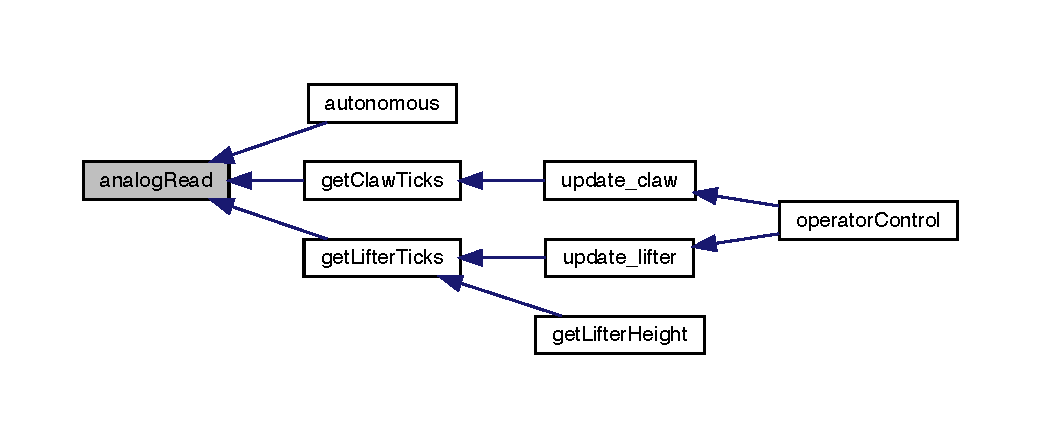
\includegraphics[width=350pt]{_a_p_i_8h_a5da86064604c539c2b6a5e2993289108_icgraph}
\end{center}
\end{figure}
\mbox{\label{_a_p_i_8h_adefc4d860dbaed441901d47d8c3598ee}} 
\index{A\+P\+I.\+h@{A\+P\+I.\+h}!analog\+Read\+Calibrated@{analog\+Read\+Calibrated}}
\index{analog\+Read\+Calibrated@{analog\+Read\+Calibrated}!A\+P\+I.\+h@{A\+P\+I.\+h}}
\paragraph{analog\+Read\+Calibrated()}
{\footnotesize\ttfamily int analog\+Read\+Calibrated (\begin{DoxyParamCaption}\item[{unsigned char}]{channel }\end{DoxyParamCaption})}

Reads the calibrated value of an analog input channel.

The \doxyref{analog\+Calibrate()}{p.}{_a_p_i_8h_aab54c390b2ff91b5b7861db877136392} function must be run first on that channel. This function is inappropriate for sensor values intended for integration, as round-\/off error can accumulate causing drift over time. Use \doxyref{analog\+Read\+Calibrated\+H\+R()}{p.}{_a_p_i_8h_a68b2c3e0863b8f4cb022fcdd77d2f5fd} instead.

This function may not work properly if the V\+EX Cortex is tethered to a PC using the orange U\+SB A to A cable and has no V\+EX 7.\+2V Battery connected and powered on, as the V\+EX Battery provides power to sensors.


\begin{DoxyParams}{Parameters}
{\em channel} & the channel to read from 1-\/8 \\
\hline
\end{DoxyParams}
\begin{DoxyReturn}{Returns}
the difference of the sensor value from its calibrated default from -\/4095 to 4095 
\end{DoxyReturn}
\mbox{\label{_a_p_i_8h_a68b2c3e0863b8f4cb022fcdd77d2f5fd}} 
\index{A\+P\+I.\+h@{A\+P\+I.\+h}!analog\+Read\+Calibrated\+HR@{analog\+Read\+Calibrated\+HR}}
\index{analog\+Read\+Calibrated\+HR@{analog\+Read\+Calibrated\+HR}!A\+P\+I.\+h@{A\+P\+I.\+h}}
\paragraph{analog\+Read\+Calibrated\+H\+R()}
{\footnotesize\ttfamily int analog\+Read\+Calibrated\+HR (\begin{DoxyParamCaption}\item[{unsigned char}]{channel }\end{DoxyParamCaption})}

Reads the calibrated value of an analog input channel 1-\/8 with enhanced precision.

The \doxyref{analog\+Calibrate()}{p.}{_a_p_i_8h_aab54c390b2ff91b5b7861db877136392} function must be run first. This is intended for integrated sensor values such as gyros and accelerometers to reduce drift due to round-\/off, and should not be used on a sensor such as a line tracker or potentiometer.

The value returned actually has 16 bits of \char`\"{}precision\char`\"{}, even though the A\+DC only reads 12 bits, so that errors induced by the average value being between two values come out in the wash when integrated over time. Think of the value as the true value times 16.

This function may not work properly if the V\+EX Cortex is tethered to a PC using the orange U\+SB A to A cable and has no V\+EX 7.\+2V Battery connected and powered on, as the V\+EX Battery provides power to sensors.


\begin{DoxyParams}{Parameters}
{\em channel} & the channel to read from 1-\/8 \\
\hline
\end{DoxyParams}
\begin{DoxyReturn}{Returns}
the difference of the sensor value from its calibrated default from -\/16384 to 16384 
\end{DoxyReturn}


Referenced by \textbf{ calculate\+\_\+accelerometer\+\_\+odemetry()}.

Here is the caller graph for this function\+:\nopagebreak
\begin{figure}[H]
\begin{center}
\leavevmode
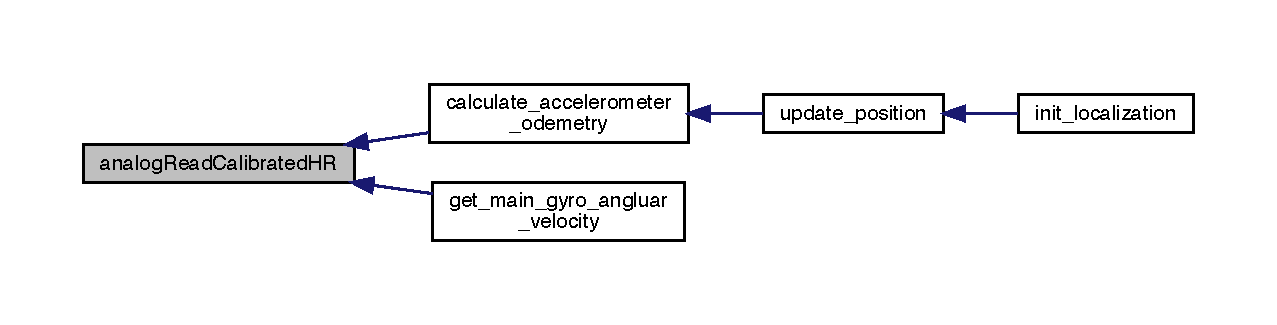
\includegraphics[width=350pt]{_a_p_i_8h_a68b2c3e0863b8f4cb022fcdd77d2f5fd_icgraph}
\end{center}
\end{figure}
\mbox{\label{_a_p_i_8h_a1c59207742a1acf45a8957d7f04f9dfe}} 
\index{A\+P\+I.\+h@{A\+P\+I.\+h}!delay@{delay}}
\index{delay@{delay}!A\+P\+I.\+h@{A\+P\+I.\+h}}
\paragraph{delay()}
{\footnotesize\ttfamily void delay (\begin{DoxyParamCaption}\item[{const unsigned long}]{time }\end{DoxyParamCaption})}

Wiring-\/compatible alias of \doxyref{task\+Delay()}{p.}{_a_p_i_8h_ac89618d0782547d189fe412a9917639b}.


\begin{DoxyParams}{Parameters}
{\em time} & the duration of the delay in milliseconds (1 000 milliseconds per second) \\
\hline
\end{DoxyParams}


Referenced by \textbf{ autonomous()}, \textbf{ display\+\_\+menu()}, \textbf{ operator\+Control()}, and \textbf{ promt\+\_\+confirmation()}.

Here is the caller graph for this function\+:\nopagebreak
\begin{figure}[H]
\begin{center}
\leavevmode
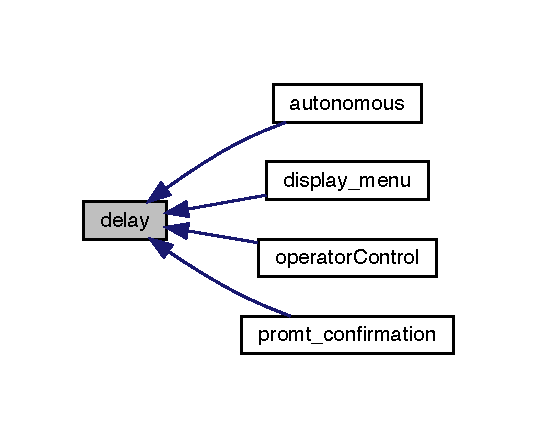
\includegraphics[width=257pt]{_a_p_i_8h_a1c59207742a1acf45a8957d7f04f9dfe_icgraph}
\end{center}
\end{figure}
\mbox{\label{_a_p_i_8h_abee651cde0a0e6ed0df34c86ed5af756}} 
\index{A\+P\+I.\+h@{A\+P\+I.\+h}!delay\+Microseconds@{delay\+Microseconds}}
\index{delay\+Microseconds@{delay\+Microseconds}!A\+P\+I.\+h@{A\+P\+I.\+h}}
\paragraph{delay\+Microseconds()}
{\footnotesize\ttfamily void delay\+Microseconds (\begin{DoxyParamCaption}\item[{const unsigned long}]{us }\end{DoxyParamCaption})}

Wait for approximately the given number of microseconds.

The method used for delaying this length of time may vary depending on the argument. The current task will always be delayed by at least the specified period, but possibly much more depending on C\+PU load. In general, this function is less reliable than \doxyref{delay()}{p.}{_a_p_i_8h_a1c59207742a1acf45a8957d7f04f9dfe}. Using this function in a loop may hog processing time from other tasks.


\begin{DoxyParams}{Parameters}
{\em us} & the duration of the delay in microseconds (1 000 000 microseconds per second) \\
\hline
\end{DoxyParams}
\mbox{\label{_a_p_i_8h_a7321930f297f38e246050f7f5b091722}} 
\index{A\+P\+I.\+h@{A\+P\+I.\+h}!digital\+Read@{digital\+Read}}
\index{digital\+Read@{digital\+Read}!A\+P\+I.\+h@{A\+P\+I.\+h}}
\paragraph{digital\+Read()}
{\footnotesize\ttfamily bool digital\+Read (\begin{DoxyParamCaption}\item[{unsigned char}]{pin }\end{DoxyParamCaption})}

Gets the digital value (1 or 0) of a pin configured as a digital input.

If the pin is configured as some other mode, the digital value which reflects the current state of the pin is returned, which may or may not differ from the currently set value. The return value is undefined for pins configured as Analog inputs, or for ports in use by a Communications interface. This function is Wiring-\/compatible.

This function may not work properly if the V\+EX Cortex is tethered to a PC using the orange U\+SB A to A cable and has no V\+EX 7.\+2V Battery connected and powered on, as the V\+EX Battery provides power to sensors.


\begin{DoxyParams}{Parameters}
{\em pin} & the pin to read from 1-\/26 \\
\hline
\end{DoxyParams}
\begin{DoxyReturn}{Returns}
true if the pin is H\+I\+GH, or false if it is L\+OW 
\end{DoxyReturn}
\mbox{\label{_a_p_i_8h_a23e767e5b47fa61d4e2cc02e6f15c7ab}} 
\index{A\+P\+I.\+h@{A\+P\+I.\+h}!digital\+Write@{digital\+Write}}
\index{digital\+Write@{digital\+Write}!A\+P\+I.\+h@{A\+P\+I.\+h}}
\paragraph{digital\+Write()}
{\footnotesize\ttfamily void digital\+Write (\begin{DoxyParamCaption}\item[{unsigned char}]{pin,  }\item[{bool}]{value }\end{DoxyParamCaption})}

Sets the digital value (1 or 0) of a pin configured as a digital output.

If the pin is configured as some other mode, behavior is undefined. This function is Wiring-\/compatible.


\begin{DoxyParams}{Parameters}
{\em pin} & the pin to write from 1-\/26 \\
\hline
{\em value} & an expression evaluating to \char`\"{}true\char`\"{} or \char`\"{}false\char`\"{} to set the output to H\+I\+GH or L\+OW respectively, or the constants H\+I\+GH or L\+OW themselves \\
\hline
\end{DoxyParams}
\mbox{\label{_a_p_i_8h_a5cfffd673e7fc8bcd1827f11b2b1490b}} 
\index{A\+P\+I.\+h@{A\+P\+I.\+h}!encoder\+Get@{encoder\+Get}}
\index{encoder\+Get@{encoder\+Get}!A\+P\+I.\+h@{A\+P\+I.\+h}}
\paragraph{encoder\+Get()}
{\footnotesize\ttfamily int encoder\+Get (\begin{DoxyParamCaption}\item[{\textbf{ Encoder}}]{enc }\end{DoxyParamCaption})}

Gets the number of ticks recorded by the encoder.

There are 360 ticks in one revolution.


\begin{DoxyParams}{Parameters}
{\em enc} & the Encoder object from \doxyref{encoder\+Init()}{p.}{_a_p_i_8h_aa68a1ba3d46d89bdb40961c52aa2c4d0} to read \\
\hline
\end{DoxyParams}
\begin{DoxyReturn}{Returns}
the signed and cumulative number of counts since the last start or reset 
\end{DoxyReturn}
\mbox{\label{_a_p_i_8h_aa68a1ba3d46d89bdb40961c52aa2c4d0}} 
\index{A\+P\+I.\+h@{A\+P\+I.\+h}!encoder\+Init@{encoder\+Init}}
\index{encoder\+Init@{encoder\+Init}!A\+P\+I.\+h@{A\+P\+I.\+h}}
\paragraph{encoder\+Init()}
{\footnotesize\ttfamily \textbf{ Encoder} encoder\+Init (\begin{DoxyParamCaption}\item[{unsigned char}]{port\+Top,  }\item[{unsigned char}]{port\+Bottom,  }\item[{bool}]{reverse }\end{DoxyParamCaption})}

Initializes and enables a quadrature encoder on two digital ports.

Neither the top port nor the bottom port can be digital port 10. N\+U\+LL will be returned if either port is invalid or the encoder is already in use. Initializing an encoder implicitly resets its count.


\begin{DoxyParams}{Parameters}
{\em port\+Top} & the \char`\"{}top\char`\"{} wire from the encoder sensor with the removable cover side UP \\
\hline
{\em port\+Bottom} & the \char`\"{}bottom\char`\"{} wire from the encoder sensor \\
\hline
{\em reverse} & if \char`\"{}true\char`\"{}, the sensor will count in the opposite direction \\
\hline
\end{DoxyParams}
\begin{DoxyReturn}{Returns}
an Encoder object to be stored and used for later calls to encoder functions 
\end{DoxyReturn}
\mbox{\label{_a_p_i_8h_a27500c21f56b2f44c62a9284ca5ebd44}} 
\index{A\+P\+I.\+h@{A\+P\+I.\+h}!encoder\+Reset@{encoder\+Reset}}
\index{encoder\+Reset@{encoder\+Reset}!A\+P\+I.\+h@{A\+P\+I.\+h}}
\paragraph{encoder\+Reset()}
{\footnotesize\ttfamily void encoder\+Reset (\begin{DoxyParamCaption}\item[{\textbf{ Encoder}}]{enc }\end{DoxyParamCaption})}

Resets the encoder to zero.

It is safe to use this method while an encoder is enabled. It is not necessary to call this method before stopping or starting an encoder.


\begin{DoxyParams}{Parameters}
{\em enc} & the Encoder object from \doxyref{encoder\+Init()}{p.}{_a_p_i_8h_aa68a1ba3d46d89bdb40961c52aa2c4d0} to reset \\
\hline
\end{DoxyParams}
\mbox{\label{_a_p_i_8h_ad068eaed82fe8c8f08ba02ea8eaf2d17}} 
\index{A\+P\+I.\+h@{A\+P\+I.\+h}!encoder\+Shutdown@{encoder\+Shutdown}}
\index{encoder\+Shutdown@{encoder\+Shutdown}!A\+P\+I.\+h@{A\+P\+I.\+h}}
\paragraph{encoder\+Shutdown()}
{\footnotesize\ttfamily void encoder\+Shutdown (\begin{DoxyParamCaption}\item[{\textbf{ Encoder}}]{enc }\end{DoxyParamCaption})}

Stops and disables the encoder.

Encoders use processing power, so disabling unused encoders increases code performance. The encoder\textquotesingle{}s count will be retained.


\begin{DoxyParams}{Parameters}
{\em enc} & the Encoder object from \doxyref{encoder\+Init()}{p.}{_a_p_i_8h_aa68a1ba3d46d89bdb40961c52aa2c4d0} to stop \\
\hline
\end{DoxyParams}
\mbox{\label{_a_p_i_8h_a0990e9bf57d497796ddcf12f61122eb5}} 
\index{A\+P\+I.\+h@{A\+P\+I.\+h}!fclose@{fclose}}
\index{fclose@{fclose}!A\+P\+I.\+h@{A\+P\+I.\+h}}
\paragraph{fclose()}
{\footnotesize\ttfamily void fclose (\begin{DoxyParamCaption}\item[{\textbf{ P\+R\+O\+S\+\_\+\+F\+I\+LE} $\ast$}]{stream }\end{DoxyParamCaption})}

Closes the specified file descriptor. This function does not work on communication ports; use \doxyref{usart\+Shutdown()}{p.}{_a_p_i_8h_a802efaab0ca93c799eb82d42cf009e07} instead.


\begin{DoxyParams}{Parameters}
{\em stream} & the file descriptor to close from \doxyref{fopen()}{p.}{_a_p_i_8h_a4cd09a1ff038c9ac9d461b077312beb6} \\
\hline
\end{DoxyParams}
\mbox{\label{_a_p_i_8h_aede7dd689fa991edc8e4c26908846606}} 
\index{A\+P\+I.\+h@{A\+P\+I.\+h}!fcount@{fcount}}
\index{fcount@{fcount}!A\+P\+I.\+h@{A\+P\+I.\+h}}
\paragraph{fcount()}
{\footnotesize\ttfamily int fcount (\begin{DoxyParamCaption}\item[{\textbf{ P\+R\+O\+S\+\_\+\+F\+I\+LE} $\ast$}]{stream }\end{DoxyParamCaption})}

Returns the number of characters that can be read without blocking (the number of characters available) from the specified stream. This only works for communication ports and files in Read mode; for files in Write mode, 0 is always returned.

This function may underestimate, but will not overestimate, the number of characters which meet this criterion.


\begin{DoxyParams}{Parameters}
{\em stream} & the stream to read (stdin, uart1, uart2, or an open file in Read mode) \\
\hline
\end{DoxyParams}
\begin{DoxyReturn}{Returns}
the number of characters which meet this criterion; if this number cannot be determined, returns 0 
\end{DoxyReturn}
\mbox{\label{_a_p_i_8h_a27fc767a71921999f9651b1ca4cf1f93}} 
\index{A\+P\+I.\+h@{A\+P\+I.\+h}!fdelete@{fdelete}}
\index{fdelete@{fdelete}!A\+P\+I.\+h@{A\+P\+I.\+h}}
\paragraph{fdelete()}
{\footnotesize\ttfamily int fdelete (\begin{DoxyParamCaption}\item[{const char $\ast$}]{file }\end{DoxyParamCaption})}

Delete the specified file if it exists and is not currently open.

The file will actually be erased from memory on the next re-\/boot. A physical power cycle is required to purge deleted files and free their allocated space for new files to be written. Deleted files are still considered inaccessible to \doxyref{fopen()}{p.}{_a_p_i_8h_a4cd09a1ff038c9ac9d461b077312beb6} in Read mode.


\begin{DoxyParams}{Parameters}
{\em file} & the file name to erase \\
\hline
\end{DoxyParams}
\begin{DoxyReturn}{Returns}
0 if the file was deleted, or 1 if the file could not be found 
\end{DoxyReturn}
\mbox{\label{_a_p_i_8h_a4c92590178e34fbedcc6fde534a0afd1}} 
\index{A\+P\+I.\+h@{A\+P\+I.\+h}!feof@{feof}}
\index{feof@{feof}!A\+P\+I.\+h@{A\+P\+I.\+h}}
\paragraph{feof()}
{\footnotesize\ttfamily int feof (\begin{DoxyParamCaption}\item[{\textbf{ P\+R\+O\+S\+\_\+\+F\+I\+LE} $\ast$}]{stream }\end{DoxyParamCaption})}

Checks to see if the specified stream is at its end. This only works for communication ports and files in Read mode; for files in Write mode, 1 is always returned.


\begin{DoxyParams}{Parameters}
{\em stream} & the channel to check (stdin, uart1, uart2, or an open file in Read mode) \\
\hline
\end{DoxyParams}
\begin{DoxyReturn}{Returns}
0 if the stream is not at E\+OF, or 1 otherwise. 
\end{DoxyReturn}
\mbox{\label{_a_p_i_8h_aec30d0b30f9f5b8a521dd8f9b6ec39c7}} 
\index{A\+P\+I.\+h@{A\+P\+I.\+h}!fflush@{fflush}}
\index{fflush@{fflush}!A\+P\+I.\+h@{A\+P\+I.\+h}}
\paragraph{fflush()}
{\footnotesize\ttfamily int fflush (\begin{DoxyParamCaption}\item[{\textbf{ P\+R\+O\+S\+\_\+\+F\+I\+LE} $\ast$}]{stream }\end{DoxyParamCaption})}

Flushes the data on the specified file channel open in Write mode. This function has no effect on a communication port or a file in Read mode, as these streams are always flushed as quickly as possible by the kernel.

Successful completion of an fflush function on a file in Write mode cannot guarantee that the file is vaild until \doxyref{fclose()}{p.}{_a_p_i_8h_a0990e9bf57d497796ddcf12f61122eb5} is used on that file descriptor.


\begin{DoxyParams}{Parameters}
{\em stream} & the channel to flush (an open file in Write mode) \\
\hline
\end{DoxyParams}
\begin{DoxyReturn}{Returns}
0 if the data was successfully flushed, E\+OF otherwise 
\end{DoxyReturn}
\mbox{\label{_a_p_i_8h_a09f27f0f85db7ff4e2d98fef10c0dde1}} 
\index{A\+P\+I.\+h@{A\+P\+I.\+h}!fgetc@{fgetc}}
\index{fgetc@{fgetc}!A\+P\+I.\+h@{A\+P\+I.\+h}}
\paragraph{fgetc()}
{\footnotesize\ttfamily int fgetc (\begin{DoxyParamCaption}\item[{\textbf{ P\+R\+O\+S\+\_\+\+F\+I\+LE} $\ast$}]{stream }\end{DoxyParamCaption})}

Reads and returns one character from the specified stream, blocking until complete.

Do not use \doxyref{fgetc()}{p.}{_a_p_i_8h_a09f27f0f85db7ff4e2d98fef10c0dde1} on a V\+EX L\+CD port; deadlock may occur.


\begin{DoxyParams}{Parameters}
{\em stream} & the stream to read (stdin, uart1, uart2, or an open file in Read mode) \\
\hline
\end{DoxyParams}
\begin{DoxyReturn}{Returns}
the next character from 0 to 255, or -\/1 if no character can be read 
\end{DoxyReturn}
\mbox{\label{_a_p_i_8h_a6315d4a637f2c6a29ad9c1355dbd6b44}} 
\index{A\+P\+I.\+h@{A\+P\+I.\+h}!fgets@{fgets}}
\index{fgets@{fgets}!A\+P\+I.\+h@{A\+P\+I.\+h}}
\paragraph{fgets()}
{\footnotesize\ttfamily char$\ast$ fgets (\begin{DoxyParamCaption}\item[{char $\ast$}]{str,  }\item[{int}]{num,  }\item[{\textbf{ P\+R\+O\+S\+\_\+\+F\+I\+LE} $\ast$}]{stream }\end{DoxyParamCaption})}

Reads a string from the specified stream, storing the characters into the memory at str. Characters will be read until the specified limit is reached, a new line is found, or the end of file is reached.

If the stream is already at end of file (for files in Read mode), N\+U\+LL will be returned; otherwise, at least one character will be read and stored into str.


\begin{DoxyParams}{Parameters}
{\em str} & the location where the characters read will be stored \\
\hline
{\em num} & the maximum number of characters to store; at most (num -\/ 1) characters will be read, with a null terminator (\textquotesingle{}\textbackslash{}0\textquotesingle{}) automatically appended \\
\hline
{\em stream} & the channel to read (stdin, uart1, uart2, or an open file in Read mode) \\
\hline
\end{DoxyParams}
\begin{DoxyReturn}{Returns}
str, or N\+U\+LL if zero characters could be read 
\end{DoxyReturn}
\mbox{\label{_a_p_i_8h_a4cd09a1ff038c9ac9d461b077312beb6}} 
\index{A\+P\+I.\+h@{A\+P\+I.\+h}!fopen@{fopen}}
\index{fopen@{fopen}!A\+P\+I.\+h@{A\+P\+I.\+h}}
\paragraph{fopen()}
{\footnotesize\ttfamily \textbf{ P\+R\+O\+S\+\_\+\+F\+I\+LE}$\ast$ fopen (\begin{DoxyParamCaption}\item[{const char $\ast$}]{file,  }\item[{const char $\ast$}]{mode }\end{DoxyParamCaption})}

Opens the given file in the specified mode. The file name is truncated to eight characters. Only four files can be in use simultaneously in any given time, with at most one of those files in Write mode. This function does not work on communication ports; use \doxyref{usart\+Init()}{p.}{_a_p_i_8h_a86066f3cf35f5fca7ec405189773182c} instead.

mode can be \char`\"{}r\char`\"{} or \char`\"{}w\char`\"{}. Due to the nature of the V\+EX Cortex memory, the \char`\"{}r+\char`\"{}, \char`\"{}w+\char`\"{}, and \char`\"{}a\char`\"{} modes are not supported by the file system.

Opening a file that does not exist in Read mode will fail and return N\+U\+LL, but opening a new file in Write mode will create it if there is space. Opening a file that already exists in Write mode will destroy the contents and create a new blank file if space is available.

There are important considerations when using of the file system on the V\+EX Cortex. Reading from files is safe, but writing to files should only be performed when robot actuators have been stopped. P\+R\+OS will attempt to continue to handle events during file writes, but most user tasks cannot execute during file writing. Powering down the V\+EX Cortex mid-\/write may cause file system corruption.


\begin{DoxyParams}{Parameters}
{\em file} & the file name \\
\hline
{\em mode} & the file mode \\
\hline
\end{DoxyParams}
\begin{DoxyReturn}{Returns}
a file descriptor pointing to the new file, or N\+U\+LL if the file could not be opened 
\end{DoxyReturn}
\mbox{\label{_a_p_i_8h_a874987bcf339f25df0bdbc24f27a03db}} 
\index{A\+P\+I.\+h@{A\+P\+I.\+h}!fprint@{fprint}}
\index{fprint@{fprint}!A\+P\+I.\+h@{A\+P\+I.\+h}}
\paragraph{fprint()}
{\footnotesize\ttfamily void fprint (\begin{DoxyParamCaption}\item[{const char $\ast$}]{string,  }\item[{\textbf{ P\+R\+O\+S\+\_\+\+F\+I\+LE} $\ast$}]{stream }\end{DoxyParamCaption})}

Prints the simple string to the specified stream.

This method is much, much faster than \doxyref{fprintf()}{p.}{_a_p_i_8h_ab9989f4619e4d3ccb13ed4c36d5f787a} and does not add a new line like \doxyref{fputs()}{p.}{_a_p_i_8h_ae4859a13f64d3dc4d57875512f0d1171}. Do not use \doxyref{fprint()}{p.}{_a_p_i_8h_a874987bcf339f25df0bdbc24f27a03db} on a V\+EX L\+CD port. Use \doxyref{lcd\+Set\+Text()}{p.}{_a_p_i_8h_a5555228be96449af952aed5bcabb6d8d} instead.


\begin{DoxyParams}{Parameters}
{\em string} & the string to write \\
\hline
{\em stream} & the stream to write (stdout, uart1, uart2, or an open file in Write mode) \\
\hline
\end{DoxyParams}
\mbox{\label{_a_p_i_8h_ab9989f4619e4d3ccb13ed4c36d5f787a}} 
\index{A\+P\+I.\+h@{A\+P\+I.\+h}!fprintf@{fprintf}}
\index{fprintf@{fprintf}!A\+P\+I.\+h@{A\+P\+I.\+h}}
\paragraph{fprintf()}
{\footnotesize\ttfamily int fprintf (\begin{DoxyParamCaption}\item[{\textbf{ P\+R\+O\+S\+\_\+\+F\+I\+LE} $\ast$}]{stream,  }\item[{const char $\ast$}]{format\+String,  }\item[{}]{... }\end{DoxyParamCaption})}

Prints the formatted string to the specified output stream.

The specifiers supported by this minimalistic \doxyref{printf()}{p.}{_a_p_i_8h_a403c82418e475fa4a8273719e6a7f3e6} function are\+:
\begin{DoxyItemize}
\item {\ttfamily \%d\+:} Signed integer in base 10 (int)
\item {\ttfamily \%u\+:} Unsigned integer in base 10 (unsigned int)
\item {\ttfamily \%x}, {\ttfamily \%X\+:} Integer in base 16 (unsigned int, int)
\item {\ttfamily \%p\+:} Pointer (void $\ast$, int $\ast$, ...)
\item {\ttfamily \%c\+:} Character (char)
\item {\ttfamily \%s\+:} Null-\/terminated string (char $\ast$)
\item {\ttfamily \%\%}\+: Single literal percent sign
\item {\ttfamily \%f\+:} Floating-\/point number
\end{DoxyItemize}

Specifiers can be modified with\+:
\begin{DoxyItemize}
\item {\ttfamily 0}\+: Zero-\/pad, instead of space-\/pad
\item {\ttfamily a.\+b\+:} Make the field at least \char`\"{}a\char`\"{} characters wide. If \char`\"{}b\char`\"{} is specified for \char`\"{}\%f\char`\"{}, changes the number of digits after the decimal point
\item {\ttfamily -\/}\+: Left-\/align, instead of right-\/align
\item {\ttfamily +}\+: Always display the sign character (displays a leading \char`\"{}+\char`\"{} for positive numbers)
\item {\ttfamily l\+:} Ignored for compatibility
\end{DoxyItemize}

Invalid format specifiers, or mismatched parameters to specifiers, cause undefined behavior. Other characters are written out verbatim. Do not use \doxyref{fprintf()}{p.}{_a_p_i_8h_ab9989f4619e4d3ccb13ed4c36d5f787a} on a V\+EX L\+CD port. Use lcd\+Print() instead.


\begin{DoxyParams}{Parameters}
{\em stream} & the stream to write (stdout, uart1, or uart2) \\
\hline
{\em format\+String} & the format string as specified above \\
\hline
\end{DoxyParams}
\begin{DoxyReturn}{Returns}
the number of characters written 
\end{DoxyReturn}


Referenced by \textbf{ assert()}.

Here is the caller graph for this function\+:\nopagebreak
\begin{figure}[H]
\begin{center}
\leavevmode
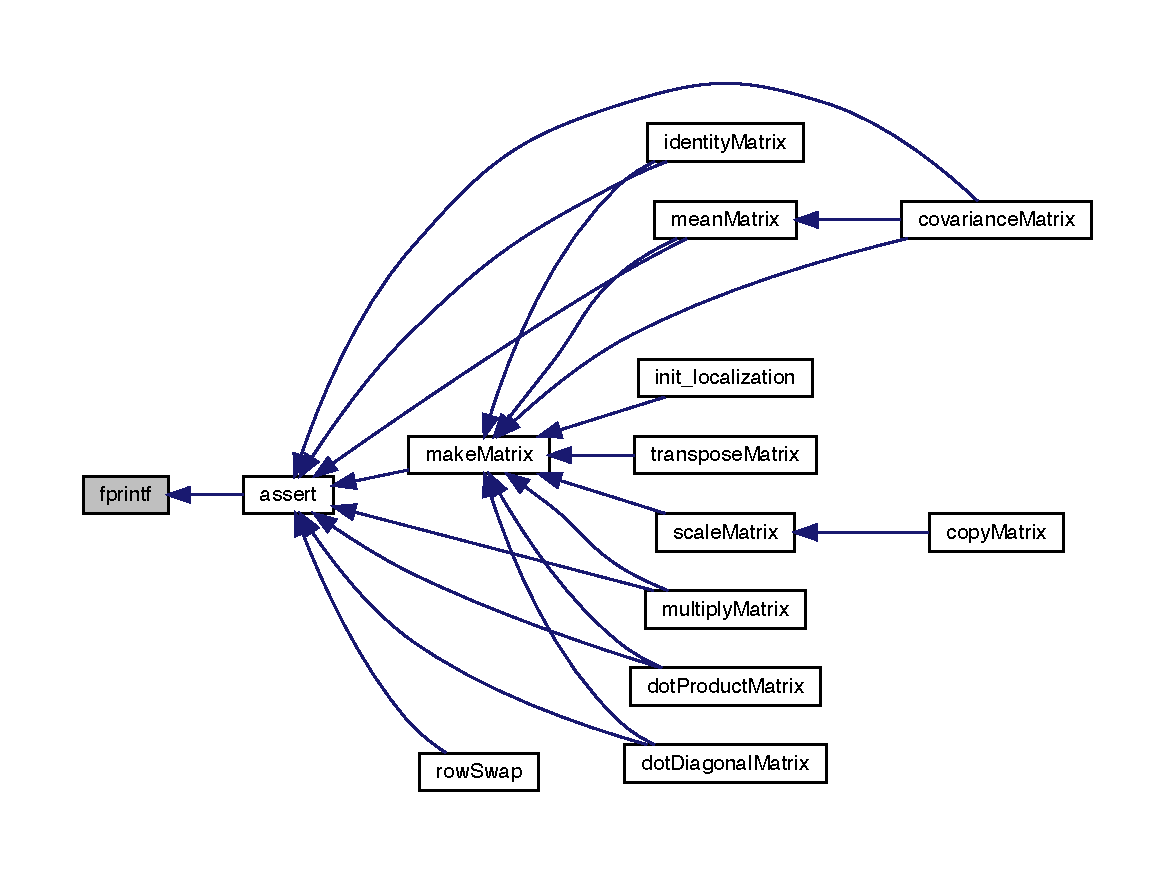
\includegraphics[width=350pt]{_a_p_i_8h_ab9989f4619e4d3ccb13ed4c36d5f787a_icgraph}
\end{center}
\end{figure}
\mbox{\label{_a_p_i_8h_afe7d25ce198da1f8fec5a2dca770cb6a}} 
\index{A\+P\+I.\+h@{A\+P\+I.\+h}!fputc@{fputc}}
\index{fputc@{fputc}!A\+P\+I.\+h@{A\+P\+I.\+h}}
\paragraph{fputc()}
{\footnotesize\ttfamily int fputc (\begin{DoxyParamCaption}\item[{int}]{value,  }\item[{\textbf{ P\+R\+O\+S\+\_\+\+F\+I\+LE} $\ast$}]{stream }\end{DoxyParamCaption})}

Writes one character to the specified stream.

Do not use \doxyref{fputc()}{p.}{_a_p_i_8h_afe7d25ce198da1f8fec5a2dca770cb6a} on a V\+EX L\+CD port. Use \doxyref{lcd\+Set\+Text()}{p.}{_a_p_i_8h_a5555228be96449af952aed5bcabb6d8d} instead.


\begin{DoxyParams}{Parameters}
{\em value} & the character to write (a value of type \char`\"{}char\char`\"{} can be used) \\
\hline
{\em stream} & the stream to write (stdout, uart1, uart2, or an open file in Write mode) \\
\hline
\end{DoxyParams}
\begin{DoxyReturn}{Returns}
the character written 
\end{DoxyReturn}
\mbox{\label{_a_p_i_8h_ae4859a13f64d3dc4d57875512f0d1171}} 
\index{A\+P\+I.\+h@{A\+P\+I.\+h}!fputs@{fputs}}
\index{fputs@{fputs}!A\+P\+I.\+h@{A\+P\+I.\+h}}
\paragraph{fputs()}
{\footnotesize\ttfamily int fputs (\begin{DoxyParamCaption}\item[{const char $\ast$}]{string,  }\item[{\textbf{ P\+R\+O\+S\+\_\+\+F\+I\+LE} $\ast$}]{stream }\end{DoxyParamCaption})}

Behaves the same as the \char`\"{}fprint\char`\"{} function, and appends a trailing newline (\char`\"{}\textbackslash{}n\char`\"{}).

Do not use \doxyref{fputs()}{p.}{_a_p_i_8h_ae4859a13f64d3dc4d57875512f0d1171} on a V\+EX L\+CD port. Use \doxyref{lcd\+Set\+Text()}{p.}{_a_p_i_8h_a5555228be96449af952aed5bcabb6d8d} instead.


\begin{DoxyParams}{Parameters}
{\em string} & the string to write \\
\hline
{\em stream} & the stream to write (stdout, uart1, uart2, or an open file in Write mode) \\
\hline
\end{DoxyParams}
\begin{DoxyReturn}{Returns}
the number of characters written, excluding the new line 
\end{DoxyReturn}
\mbox{\label{_a_p_i_8h_a01b4329a6303387a4187c94343c0cc59}} 
\index{A\+P\+I.\+h@{A\+P\+I.\+h}!fread@{fread}}
\index{fread@{fread}!A\+P\+I.\+h@{A\+P\+I.\+h}}
\paragraph{fread()}
{\footnotesize\ttfamily size\+\_\+t fread (\begin{DoxyParamCaption}\item[{void $\ast$}]{ptr,  }\item[{size\+\_\+t}]{size,  }\item[{size\+\_\+t}]{count,  }\item[{\textbf{ P\+R\+O\+S\+\_\+\+F\+I\+LE} $\ast$}]{stream }\end{DoxyParamCaption})}

Reads data from a stream into memory. Returns the number of bytes thus read.

If the memory at ptr cannot store (size $\ast$ count) bytes, undefined behavior occurs.


\begin{DoxyParams}{Parameters}
{\em ptr} & a pointer to where the data will be stored \\
\hline
{\em size} & the size of each data element to read in bytes \\
\hline
{\em count} & the number of data elements to read \\
\hline
{\em stream} & the stream to read (stdout, uart1, uart2, or an open file in Read mode) \\
\hline
\end{DoxyParams}
\begin{DoxyReturn}{Returns}
the number of bytes successfully read 
\end{DoxyReturn}
\mbox{\label{_a_p_i_8h_adda53be8dacaa9deab92cabb9f2e54dd}} 
\index{A\+P\+I.\+h@{A\+P\+I.\+h}!fseek@{fseek}}
\index{fseek@{fseek}!A\+P\+I.\+h@{A\+P\+I.\+h}}
\paragraph{fseek()}
{\footnotesize\ttfamily int fseek (\begin{DoxyParamCaption}\item[{\textbf{ P\+R\+O\+S\+\_\+\+F\+I\+LE} $\ast$}]{stream,  }\item[{long int}]{offset,  }\item[{int}]{origin }\end{DoxyParamCaption})}

Seeks within a file open in Read mode. This function will fail when used on a file in Write mode or on any communications port.


\begin{DoxyParams}{Parameters}
{\em stream} & the stream to seek within \\
\hline
{\em offset} & the location within the stream to seek \\
\hline
{\em origin} & the reference location for offset\+: S\+E\+E\+K\+\_\+\+C\+UR, S\+E\+E\+K\+\_\+\+S\+ET, or S\+E\+E\+K\+\_\+\+E\+ND \\
\hline
\end{DoxyParams}
\begin{DoxyReturn}{Returns}
0 if the seek was successful, or 1 otherwise 
\end{DoxyReturn}
\mbox{\label{_a_p_i_8h_a1c2742ed272f2a5e12962df45653ff18}} 
\index{A\+P\+I.\+h@{A\+P\+I.\+h}!ftell@{ftell}}
\index{ftell@{ftell}!A\+P\+I.\+h@{A\+P\+I.\+h}}
\paragraph{ftell()}
{\footnotesize\ttfamily long int ftell (\begin{DoxyParamCaption}\item[{\textbf{ P\+R\+O\+S\+\_\+\+F\+I\+LE} $\ast$}]{stream }\end{DoxyParamCaption})}

Returns the current position of the stream. This function works on files in either Read or Write mode, but will fail on communications ports.


\begin{DoxyParams}{Parameters}
{\em stream} & the stream to check \\
\hline
\end{DoxyParams}
\begin{DoxyReturn}{Returns}
the offset of the stream, or -\/1 if the offset could not be determined 
\end{DoxyReturn}
\mbox{\label{_a_p_i_8h_aaadc510ae9d7c433161a366de9fb828d}} 
\index{A\+P\+I.\+h@{A\+P\+I.\+h}!fwrite@{fwrite}}
\index{fwrite@{fwrite}!A\+P\+I.\+h@{A\+P\+I.\+h}}
\paragraph{fwrite()}
{\footnotesize\ttfamily size\+\_\+t fwrite (\begin{DoxyParamCaption}\item[{const void $\ast$}]{ptr,  }\item[{size\+\_\+t}]{size,  }\item[{size\+\_\+t}]{count,  }\item[{\textbf{ P\+R\+O\+S\+\_\+\+F\+I\+LE} $\ast$}]{stream }\end{DoxyParamCaption})}

Writes data from memory to a stream. Returns the number of bytes thus written.

If the memory at ptr is not as long as (size $\ast$ count) bytes, undefined behavior occurs.


\begin{DoxyParams}{Parameters}
{\em ptr} & a pointer to the data to write \\
\hline
{\em size} & the size of each data element to write in bytes \\
\hline
{\em count} & the number of data elements to write \\
\hline
{\em stream} & the stream to write (stdout, uart1, uart2, or an open file in Write mode) \\
\hline
\end{DoxyParams}
\begin{DoxyReturn}{Returns}
the number of bytes successfully written 
\end{DoxyReturn}
\mbox{\label{_a_p_i_8h_ac45fdeab51c3197c1e7c4ec7beabaca9}} 
\index{A\+P\+I.\+h@{A\+P\+I.\+h}!getchar@{getchar}}
\index{getchar@{getchar}!A\+P\+I.\+h@{A\+P\+I.\+h}}
\paragraph{getchar()}
{\footnotesize\ttfamily int getchar (\begin{DoxyParamCaption}{ }\end{DoxyParamCaption})}

Reads and returns one character from \char`\"{}stdin\char`\"{}, which is the PC debug terminal.

\begin{DoxyReturn}{Returns}
the next character from 0 to 255, or -\/1 if no character can be read 
\end{DoxyReturn}
\mbox{\label{_a_p_i_8h_a0ae2ca5d2fd99f33aaef38786bb8ee59}} 
\index{A\+P\+I.\+h@{A\+P\+I.\+h}!gyro\+Get@{gyro\+Get}}
\index{gyro\+Get@{gyro\+Get}!A\+P\+I.\+h@{A\+P\+I.\+h}}
\paragraph{gyro\+Get()}
{\footnotesize\ttfamily int gyro\+Get (\begin{DoxyParamCaption}\item[{\textbf{ Gyro}}]{gyro }\end{DoxyParamCaption})}

Gets the current gyro angle in degrees, rounded to the nearest degree.

There are 360 degrees in a circle.


\begin{DoxyParams}{Parameters}
{\em gyro} & the Gyro object from \doxyref{gyro\+Init()}{p.}{_a_p_i_8h_a17270080a32b64937a3669089a80120f} to read \\
\hline
\end{DoxyParams}
\begin{DoxyReturn}{Returns}
the signed and cumulative number of degrees rotated around the gyro\textquotesingle{}s vertical axis since the last start or reset 
\end{DoxyReturn}


Referenced by \textbf{ calculate\+\_\+gryo\+\_\+anglular\+\_\+velocity()}.

Here is the caller graph for this function\+:\nopagebreak
\begin{figure}[H]
\begin{center}
\leavevmode
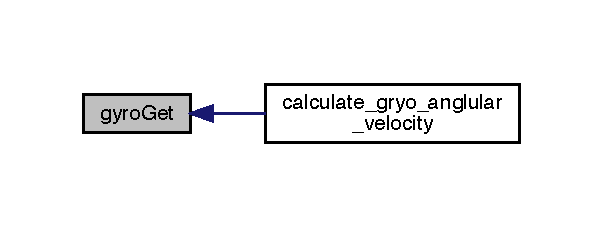
\includegraphics[width=289pt]{_a_p_i_8h_a0ae2ca5d2fd99f33aaef38786bb8ee59_icgraph}
\end{center}
\end{figure}
\mbox{\label{_a_p_i_8h_a17270080a32b64937a3669089a80120f}} 
\index{A\+P\+I.\+h@{A\+P\+I.\+h}!gyro\+Init@{gyro\+Init}}
\index{gyro\+Init@{gyro\+Init}!A\+P\+I.\+h@{A\+P\+I.\+h}}
\paragraph{gyro\+Init()}
{\footnotesize\ttfamily \textbf{ Gyro} gyro\+Init (\begin{DoxyParamCaption}\item[{unsigned char}]{port,  }\item[{unsigned short}]{multiplier }\end{DoxyParamCaption})}

Initializes and enables a gyro on an analog port.

N\+U\+LL will be returned if the port is invalid or the gyro is already in use. Initializing a gyro implicitly calibrates it and resets its count. Do not move the robot while the gyro is being calibrated. It is suggested to call this function in \doxyref{initialize()}{p.}{main_8h_a25a40b6614565f755233080a384c35f1} and to place the robot in its final position before powering it on.

The multiplier parameter can tune the gyro to adapt to specific sensors. The default value at this time is 196; higher values will increase the number of degrees reported for a fixed actual rotation, while lower values will decrease the number of degrees reported. If your robot is consistently turning too far, increase the multiplier, and if it is not turning far enough, decrease the multiplier.


\begin{DoxyParams}{Parameters}
{\em port} & the analog port to use from 1-\/8 \\
\hline
{\em multiplier} & an optional constant to tune the gyro readings; use 0 for the default value \\
\hline
\end{DoxyParams}
\begin{DoxyReturn}{Returns}
a Gyro object to be stored and used for later calls to gyro functions 
\end{DoxyReturn}


Referenced by \textbf{ init\+\_\+localization()}.

Here is the caller graph for this function\+:\nopagebreak
\begin{figure}[H]
\begin{center}
\leavevmode
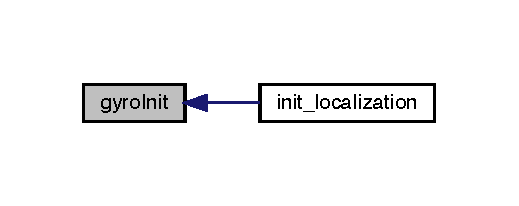
\includegraphics[width=249pt]{_a_p_i_8h_a17270080a32b64937a3669089a80120f_icgraph}
\end{center}
\end{figure}
\mbox{\label{_a_p_i_8h_a5de4afb9c6bd747e8d7664e1c72390b2}} 
\index{A\+P\+I.\+h@{A\+P\+I.\+h}!gyro\+Reset@{gyro\+Reset}}
\index{gyro\+Reset@{gyro\+Reset}!A\+P\+I.\+h@{A\+P\+I.\+h}}
\paragraph{gyro\+Reset()}
{\footnotesize\ttfamily void gyro\+Reset (\begin{DoxyParamCaption}\item[{\textbf{ Gyro}}]{gyro }\end{DoxyParamCaption})}

Resets the gyro to zero.

It is safe to use this method while a gyro is enabled. It is not necessary to call this method before stopping or starting a gyro.


\begin{DoxyParams}{Parameters}
{\em gyro} & the Gyro object from \doxyref{gyro\+Init()}{p.}{_a_p_i_8h_a17270080a32b64937a3669089a80120f} to reset \\
\hline
\end{DoxyParams}
\mbox{\label{_a_p_i_8h_a4e50e79b76d956dd9d466a582a5bb7b5}} 
\index{A\+P\+I.\+h@{A\+P\+I.\+h}!gyro\+Shutdown@{gyro\+Shutdown}}
\index{gyro\+Shutdown@{gyro\+Shutdown}!A\+P\+I.\+h@{A\+P\+I.\+h}}
\paragraph{gyro\+Shutdown()}
{\footnotesize\ttfamily void gyro\+Shutdown (\begin{DoxyParamCaption}\item[{\textbf{ Gyro}}]{gyro }\end{DoxyParamCaption})}

Stops and disables the gyro.

Gyros use processing power, so disabling unused gyros increases code performance. The gyro\textquotesingle{}s position will be retained.


\begin{DoxyParams}{Parameters}
{\em gyro} & the Gyro object from \doxyref{gyro\+Init()}{p.}{_a_p_i_8h_a17270080a32b64937a3669089a80120f} to stop \\
\hline
\end{DoxyParams}
\mbox{\label{_a_p_i_8h_a591bdbd4df72ac4231feba723faac640}} 
\index{A\+P\+I.\+h@{A\+P\+I.\+h}!i2c\+Read@{i2c\+Read}}
\index{i2c\+Read@{i2c\+Read}!A\+P\+I.\+h@{A\+P\+I.\+h}}
\paragraph{i2c\+Read()}
{\footnotesize\ttfamily bool i2c\+Read (\begin{DoxyParamCaption}\item[{uint8\+\_\+t}]{addr,  }\item[{uint8\+\_\+t $\ast$}]{data,  }\item[{uint16\+\_\+t}]{count }\end{DoxyParamCaption})}

i2c\+Read -\/ Reads the specified number of data bytes from the specified 7-\/bit I2C address. The bytes will be stored at the specified location. Returns true if successful or false if failed. If only some bytes could be read, false is still returned.

The I2C address should be right-\/aligned; the R/W bit is automatically supplied.

Since most I2C devices use an 8-\/bit register architecture, this method has limited usefulness. Consider i2c\+Read\+Register instead for the vast majority of applications. \mbox{\label{_a_p_i_8h_a69670b44b640e824da387a6616dc2f9a}} 
\index{A\+P\+I.\+h@{A\+P\+I.\+h}!i2c\+Read\+Register@{i2c\+Read\+Register}}
\index{i2c\+Read\+Register@{i2c\+Read\+Register}!A\+P\+I.\+h@{A\+P\+I.\+h}}
\paragraph{i2c\+Read\+Register()}
{\footnotesize\ttfamily bool i2c\+Read\+Register (\begin{DoxyParamCaption}\item[{uint8\+\_\+t}]{addr,  }\item[{uint8\+\_\+t}]{reg,  }\item[{uint8\+\_\+t $\ast$}]{value,  }\item[{uint16\+\_\+t}]{count }\end{DoxyParamCaption})}

i2c\+Read\+Register -\/ Reads the specified amount of data from the given register address on the specified 7-\/bit I2C address. Returns true if successful or false if failed. If only some bytes could be read, false is still returned.

The I2C address should be right-\/aligned; the R/W bit is automatically supplied.

Most I2C devices support an auto-\/increment address feature, so using this method to read more than one byte will usually read a block of sequential registers. Try to merge reads to separate registers into a larger read using this function whenever possible to improve code reliability, even if a few intermediate values need to be thrown away. \mbox{\label{_a_p_i_8h_a2d286627370658ecee04a18335b91c39}} 
\index{A\+P\+I.\+h@{A\+P\+I.\+h}!i2c\+Write@{i2c\+Write}}
\index{i2c\+Write@{i2c\+Write}!A\+P\+I.\+h@{A\+P\+I.\+h}}
\paragraph{i2c\+Write()}
{\footnotesize\ttfamily bool i2c\+Write (\begin{DoxyParamCaption}\item[{uint8\+\_\+t}]{addr,  }\item[{uint8\+\_\+t $\ast$}]{data,  }\item[{uint16\+\_\+t}]{count }\end{DoxyParamCaption})}

i2c\+Write -\/ Writes the specified number of data bytes to the specified 7-\/bit I2C address. Returns true if successful or false if failed. If only smoe bytes could be written, false is still returned.

The I2C address should be right-\/aligned; the R/W bit is automatically supplied.

Since most I2C devices use an 8-\/bit register architecture, this method is mostly useful for setting the register position (most devices remember the last-\/used address) or writing a sequence of bytes to one register address using an auto-\/increment feature. In these cases, the first byte written from the data buffer should have the register address to use. \mbox{\label{_a_p_i_8h_a51385d22e08f52852c85ad675e3523a9}} 
\index{A\+P\+I.\+h@{A\+P\+I.\+h}!i2c\+Write\+Register@{i2c\+Write\+Register}}
\index{i2c\+Write\+Register@{i2c\+Write\+Register}!A\+P\+I.\+h@{A\+P\+I.\+h}}
\paragraph{i2c\+Write\+Register()}
{\footnotesize\ttfamily bool i2c\+Write\+Register (\begin{DoxyParamCaption}\item[{uint8\+\_\+t}]{addr,  }\item[{uint8\+\_\+t}]{reg,  }\item[{uint16\+\_\+t}]{value }\end{DoxyParamCaption})}

i2c\+Write\+Register -\/ Writes the specified data byte to a register address on the specified 7-\/bit I2C address. Returns true if successful or false if failed.

The I2C address should be right-\/aligned; the R/W bit is automatically supplied.

Only one byte can be written to each register address using this method. While useful for the vast majority of I2C operations, writing multiple bytes requires the i2c\+Write method. \mbox{\label{_a_p_i_8h_ac4f1500418a729ac3ee95bce9768b20c}} 
\index{A\+P\+I.\+h@{A\+P\+I.\+h}!ime\+Get@{ime\+Get}}
\index{ime\+Get@{ime\+Get}!A\+P\+I.\+h@{A\+P\+I.\+h}}
\paragraph{ime\+Get()}
{\footnotesize\ttfamily bool ime\+Get (\begin{DoxyParamCaption}\item[{unsigned char}]{address,  }\item[{int $\ast$}]{value }\end{DoxyParamCaption})}

Gets the current 32-\/bit count of the specified I\+ME.

Much like the count for a quadrature encoder, the tick count is signed and cumulative. The value reflects total counts since the last reset. Different V\+EX Motor Encoders have a different number of counts per revolution\+:


\begin{DoxyItemize}
\item {\ttfamily 240.\+448} for the 269 I\+ME
\item {\ttfamily 627.\+2} for the 393 I\+ME in high torque mode (factory default)
\item {\ttfamily 392} for the 393 I\+ME in high speed mode
\end{DoxyItemize}

If the I\+ME address is invalid, or the I\+ME has not been reset or initialized, the value stored in $\ast$value is undefined.


\begin{DoxyParams}{Parameters}
{\em address} & the I\+ME address to fetch from 0 to I\+M\+E\+\_\+\+A\+D\+D\+R\+\_\+\+M\+AX \\
\hline
{\em value} & a pointer to the location where the value will be stored (obtained using the \char`\"{}\&\char`\"{} operator on the target variable name e.\+g. {\ttfamily ime\+Get(2, \&counts)}) \\
\hline
\end{DoxyParams}
\begin{DoxyReturn}{Returns}
true if the count was successfully read and the value stored in $\ast$value is valid; false otherwise 
\end{DoxyReturn}


Referenced by \textbf{ autonomous()}, and \textbf{ get\+\_\+encoder\+\_\+ticks()}.

Here is the caller graph for this function\+:\nopagebreak
\begin{figure}[H]
\begin{center}
\leavevmode
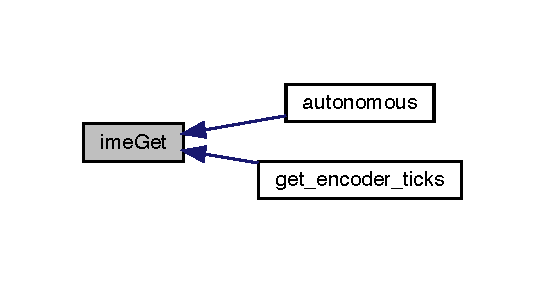
\includegraphics[width=261pt]{_a_p_i_8h_ac4f1500418a729ac3ee95bce9768b20c_icgraph}
\end{center}
\end{figure}
\mbox{\label{_a_p_i_8h_a2dfd22ed31510b48a91bd9cd3d04a72f}} 
\index{A\+P\+I.\+h@{A\+P\+I.\+h}!ime\+Get\+Velocity@{ime\+Get\+Velocity}}
\index{ime\+Get\+Velocity@{ime\+Get\+Velocity}!A\+P\+I.\+h@{A\+P\+I.\+h}}
\paragraph{ime\+Get\+Velocity()}
{\footnotesize\ttfamily bool ime\+Get\+Velocity (\begin{DoxyParamCaption}\item[{unsigned char}]{address,  }\item[{int $\ast$}]{value }\end{DoxyParamCaption})}

Gets the current rotational velocity of the specified I\+ME.

In this version of P\+R\+OS, the velocity is positive if the I\+ME count is increasing and negative if the I\+ME count is decreasing. The velocity is in R\+PM of the internal encoder wheel. Since checking the I\+ME for its type cannot reveal whether the motor gearing is high speed or high torque (in the 2-\/\+Wire Motor 393 case), the user must divide the return value by the number of output revolutions per encoder revolution\+:


\begin{DoxyItemize}
\item {\ttfamily 30.\+056} for the 269 I\+ME
\item {\ttfamily 39.\+2} for the 393 I\+ME in high torque mode (factory default)
\item {\ttfamily 24.\+5} for the 393 I\+ME in high speed mode
\end{DoxyItemize}

If the I\+ME address is invalid, or the I\+ME has not been reset or initialized, the value stored in $\ast$value is undefined.


\begin{DoxyParams}{Parameters}
{\em address} & the I\+ME address to fetch from 0 to I\+M\+E\+\_\+\+A\+D\+D\+R\+\_\+\+M\+AX \\
\hline
{\em value} & a pointer to the location where the value will be stored (obtained using the \char`\"{}\&\char`\"{} operator on the target variable name e.\+g. {\ttfamily ime\+Get\+Velocity(2, \&counts)}) \\
\hline
\end{DoxyParams}
\begin{DoxyReturn}{Returns}
true if the velocity was successfully read and the value stored in $\ast$value is valid; false otherwise 
\end{DoxyReturn}


Referenced by \textbf{ get\+\_\+encoder\+\_\+velocity()}.

Here is the caller graph for this function\+:\nopagebreak
\begin{figure}[H]
\begin{center}
\leavevmode
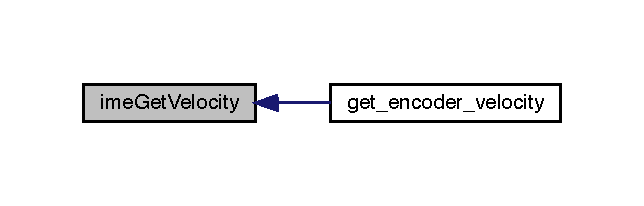
\includegraphics[width=309pt]{_a_p_i_8h_a2dfd22ed31510b48a91bd9cd3d04a72f_icgraph}
\end{center}
\end{figure}
\mbox{\label{_a_p_i_8h_a868ab46aa5992e60829936c0109160bf}} 
\index{A\+P\+I.\+h@{A\+P\+I.\+h}!ime\+Initialize\+All@{ime\+Initialize\+All}}
\index{ime\+Initialize\+All@{ime\+Initialize\+All}!A\+P\+I.\+h@{A\+P\+I.\+h}}
\paragraph{ime\+Initialize\+All()}
{\footnotesize\ttfamily unsigned int ime\+Initialize\+All (\begin{DoxyParamCaption}{ }\end{DoxyParamCaption})}

Initializes all I\+M\+Es.

I\+M\+Es are assigned sequential incrementing addresses, beginning with the first I\+ME on the chain (closest to the V\+EX Cortex I2C port). Therefore, a given configuration of I\+M\+Es will always have the same ID assigned to each encoder. The addresses range from 0 to I\+M\+E\+\_\+\+A\+D\+D\+R\+\_\+\+M\+AX, so the first encoder gets 0, the second gets 1, ...

This function should most likely be used in \doxyref{initialize()}{p.}{main_8h_a25a40b6614565f755233080a384c35f1}. Do not use it in \doxyref{initialize\+I\+O()}{p.}{main_8h_ad9cda921edb01125bb13c2f86bcf624b} or at any other time when the scheduler is paused (like an interrupt). Checking the return value of this function is important to ensure that all I\+M\+Es are plugged in and responding as expected.

This function, unlike the other I\+ME functions, is not thread safe. If using ime\+Initialize\+All to re-\/initialize encoders, calls to other I\+ME functions might behave unpredictably during this function\textquotesingle{}s execution.

\begin{DoxyReturn}{Returns}
the number of I\+M\+Es successfully initialized. 
\end{DoxyReturn}


Referenced by \textbf{ init\+\_\+encoders()}, and \textbf{ initialize()}.

Here is the caller graph for this function\+:\nopagebreak
\begin{figure}[H]
\begin{center}
\leavevmode
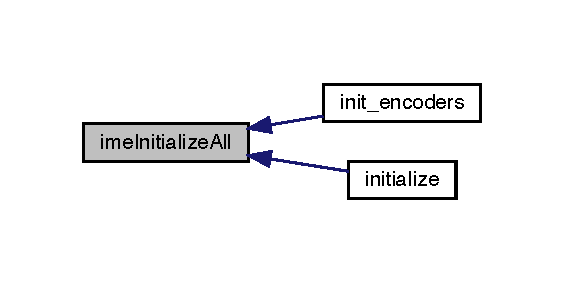
\includegraphics[width=271pt]{_a_p_i_8h_a868ab46aa5992e60829936c0109160bf_icgraph}
\end{center}
\end{figure}
\mbox{\label{_a_p_i_8h_ab1ef9ee5f8878856896a6c920ed762fc}} 
\index{A\+P\+I.\+h@{A\+P\+I.\+h}!ime\+Reset@{ime\+Reset}}
\index{ime\+Reset@{ime\+Reset}!A\+P\+I.\+h@{A\+P\+I.\+h}}
\paragraph{ime\+Reset()}
{\footnotesize\ttfamily bool ime\+Reset (\begin{DoxyParamCaption}\item[{unsigned char}]{address }\end{DoxyParamCaption})}

Resets the specified I\+ME\textquotesingle{}s counters to zero.

This method can be used while the I\+ME is rotating.


\begin{DoxyParams}{Parameters}
{\em address} & the I\+ME address to reset from 0 to I\+M\+E\+\_\+\+A\+D\+D\+R\+\_\+\+M\+AX \\
\hline
\end{DoxyParams}
\begin{DoxyReturn}{Returns}
true if the reset succeeded; false otherwise 
\end{DoxyReturn}


Referenced by \textbf{ autonomous()}.

Here is the caller graph for this function\+:\nopagebreak
\begin{figure}[H]
\begin{center}
\leavevmode
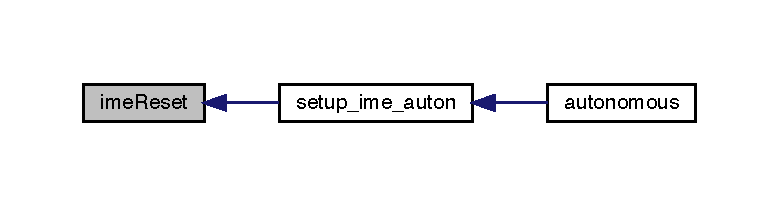
\includegraphics[width=245pt]{_a_p_i_8h_ab1ef9ee5f8878856896a6c920ed762fc_icgraph}
\end{center}
\end{figure}
\mbox{\label{_a_p_i_8h_a19de5a557348a6b4931c89eb82eb8fb7}} 
\index{A\+P\+I.\+h@{A\+P\+I.\+h}!ime\+Shutdown@{ime\+Shutdown}}
\index{ime\+Shutdown@{ime\+Shutdown}!A\+P\+I.\+h@{A\+P\+I.\+h}}
\paragraph{ime\+Shutdown()}
{\footnotesize\ttfamily void ime\+Shutdown (\begin{DoxyParamCaption}{ }\end{DoxyParamCaption})}

Shuts down all I\+M\+Es on the chain; their addresses return to the default and the stored counts and velocities are lost. This function, unlike the other I\+ME functions, is not thread safe.

To use the I\+ME chain again, wait at least 0.\+25 seconds before using ime\+Initialize\+All again. \mbox{\label{_a_p_i_8h_a9291f71712cfb21e9bfd51682260fa73}} 
\index{A\+P\+I.\+h@{A\+P\+I.\+h}!io\+Clear\+Interrupt@{io\+Clear\+Interrupt}}
\index{io\+Clear\+Interrupt@{io\+Clear\+Interrupt}!A\+P\+I.\+h@{A\+P\+I.\+h}}
\paragraph{io\+Clear\+Interrupt()}
{\footnotesize\ttfamily void io\+Clear\+Interrupt (\begin{DoxyParamCaption}\item[{unsigned char}]{pin }\end{DoxyParamCaption})}

Disables interrupts on the specified pin.

Disabling interrupts on interrupt pins which are not in use conserves processing time.


\begin{DoxyParams}{Parameters}
{\em pin} & the pin on which to reset interrupts from 1-\/9,11-\/12 \\
\hline
\end{DoxyParams}
\mbox{\label{_a_p_i_8h_a8d0fd8e69a4c4c5aba981d106ee7f9ac}} 
\index{A\+P\+I.\+h@{A\+P\+I.\+h}!io\+Set\+Interrupt@{io\+Set\+Interrupt}}
\index{io\+Set\+Interrupt@{io\+Set\+Interrupt}!A\+P\+I.\+h@{A\+P\+I.\+h}}
\paragraph{io\+Set\+Interrupt()}
{\footnotesize\ttfamily void io\+Set\+Interrupt (\begin{DoxyParamCaption}\item[{unsigned char}]{pin,  }\item[{unsigned char}]{edges,  }\item[{\textbf{ Interrupt\+Handler}}]{handler }\end{DoxyParamCaption})}

Sets up an interrupt to occur on the specified pin, and resets any counters or timers associated with the pin.

Each time the specified change occurs, the function pointer passed in will be called with the pin that changed as an argument. Enabling pin-\/change interrupts consumes processing time, so it is best to only enable necessary interrupts and to keep the Interrupt\+Handler function short. Pin change interrupts can only be enabled on pins 1-\/9 and 11-\/12.

Do not use A\+PI functions such as \doxyref{delay()}{p.}{_a_p_i_8h_a1c59207742a1acf45a8957d7f04f9dfe} inside the handler function, as the function will run in an I\+SR where the scheduler is paused and no other interrupts can execute. It is best to quickly update some state and allow a task to perform the work.

Do not use this function on pins that are also being used by the built-\/in ultrasonic or shaft encoder drivers, or on pins which have been switched to output mode.


\begin{DoxyParams}{Parameters}
{\em pin} & the pin on which to enable interrupts from 1-\/9,11-\/12 \\
\hline
{\em edges} & one of I\+N\+T\+E\+R\+R\+U\+P\+T\+\_\+\+E\+D\+G\+E\+\_\+\+R\+I\+S\+I\+NG, I\+N\+T\+E\+R\+R\+U\+P\+T\+\_\+\+E\+D\+G\+E\+\_\+\+F\+A\+L\+L\+I\+NG, or I\+N\+T\+E\+R\+R\+U\+P\+T\+\_\+\+E\+D\+G\+E\+\_\+\+B\+O\+TH \\
\hline
{\em handler} & the function to call when the condition is satisfied \\
\hline
\end{DoxyParams}
\mbox{\label{_a_p_i_8h_aad3f43faea37dc2eddaf4ba0926a511f}} 
\index{A\+P\+I.\+h@{A\+P\+I.\+h}!is\+Autonomous@{is\+Autonomous}}
\index{is\+Autonomous@{is\+Autonomous}!A\+P\+I.\+h@{A\+P\+I.\+h}}
\paragraph{is\+Autonomous()}
{\footnotesize\ttfamily bool is\+Autonomous (\begin{DoxyParamCaption}{ }\end{DoxyParamCaption})}

Returns true if the robot is in autonomous mode, or false otherwise.

While in autonomous mode, joystick inputs will return a neutral value, but serial port communications (even over Vex\+N\+ET) will still work properly. \mbox{\label{_a_p_i_8h_a56722b6f1c22da04885bc9853148bb71}} 
\index{A\+P\+I.\+h@{A\+P\+I.\+h}!is\+Enabled@{is\+Enabled}}
\index{is\+Enabled@{is\+Enabled}!A\+P\+I.\+h@{A\+P\+I.\+h}}
\paragraph{is\+Enabled()}
{\footnotesize\ttfamily bool is\+Enabled (\begin{DoxyParamCaption}{ }\end{DoxyParamCaption})}

Returns true if the robot is enabled, or false otherwise.

While disabled via the V\+EX Competition Switch or V\+EX Field Controller, motors will not function. However, the digital I/O ports can still be changed, which may indirectly affect the robot state (e.\+g. solenoids). Avoid performing externally visible actions while disabled (the kernel should take care of this most of the time). 

Referenced by \textbf{ display\+\_\+menu()}.

Here is the caller graph for this function\+:\nopagebreak
\begin{figure}[H]
\begin{center}
\leavevmode
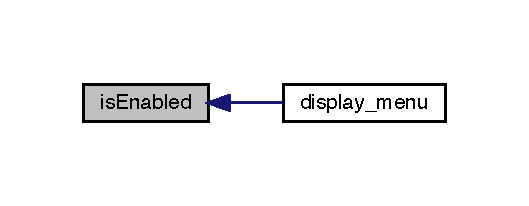
\includegraphics[width=254pt]{_a_p_i_8h_a56722b6f1c22da04885bc9853148bb71_icgraph}
\end{center}
\end{figure}
\mbox{\label{_a_p_i_8h_a72aa0bce6b1d8ee298a60617f8fa74da}} 
\index{A\+P\+I.\+h@{A\+P\+I.\+h}!is\+Joystick\+Connected@{is\+Joystick\+Connected}}
\index{is\+Joystick\+Connected@{is\+Joystick\+Connected}!A\+P\+I.\+h@{A\+P\+I.\+h}}
\paragraph{is\+Joystick\+Connected()}
{\footnotesize\ttfamily bool is\+Joystick\+Connected (\begin{DoxyParamCaption}\item[{unsigned char}]{joystick }\end{DoxyParamCaption})}

Returns true if a joystick is connected to the specified slot number (1 or 2), or false otherwise.

Useful for automatically merging joysticks for one operator, or splitting for two. This function does not work properly during \doxyref{initialize()}{p.}{main_8h_a25a40b6614565f755233080a384c35f1} or \doxyref{initialize\+I\+O()}{p.}{main_8h_ad9cda921edb01125bb13c2f86bcf624b} and can return false positives. It should be checked once and stored at the beginning of \doxyref{operator\+Control()}{p.}{main_8h_ac71a94af413917f27d108e95c4d6f6a7}.


\begin{DoxyParams}{Parameters}
{\em joystick} & the joystick slot to check \\
\hline
\end{DoxyParams}
\mbox{\label{_a_p_i_8h_a1eceab28885f971892b9d4fc76e0e542}} 
\index{A\+P\+I.\+h@{A\+P\+I.\+h}!is\+Online@{is\+Online}}
\index{is\+Online@{is\+Online}!A\+P\+I.\+h@{A\+P\+I.\+h}}
\paragraph{is\+Online()}
{\footnotesize\ttfamily bool is\+Online (\begin{DoxyParamCaption}{ }\end{DoxyParamCaption})}

Returns true if a V\+EX field controller or competition switch is connected, or false otherwise.

When in online mode, the switching between \doxyref{autonomous()}{p.}{main_8h_a3c7ca506bbc071fa740de13805b7f376} and \doxyref{operator\+Control()}{p.}{main_8h_ac71a94af413917f27d108e95c4d6f6a7} tasks is managed by the P\+R\+OS kernel. \mbox{\label{_a_p_i_8h_ad56fcec15d1a48deb8780bb0fc38be4d}} 
\index{A\+P\+I.\+h@{A\+P\+I.\+h}!joystick\+Get\+Analog@{joystick\+Get\+Analog}}
\index{joystick\+Get\+Analog@{joystick\+Get\+Analog}!A\+P\+I.\+h@{A\+P\+I.\+h}}
\paragraph{joystick\+Get\+Analog()}
{\footnotesize\ttfamily int joystick\+Get\+Analog (\begin{DoxyParamCaption}\item[{unsigned char}]{joystick,  }\item[{unsigned char}]{axis }\end{DoxyParamCaption})}

Gets the value of a control axis on the V\+EX joystick. Returns the value from -\/127 to 127, or 0 if no joystick is connected to the requested slot.


\begin{DoxyParams}{Parameters}
{\em joystick} & the joystick slot to check \\
\hline
{\em axis} & one of 1, 2, 3, 4, A\+C\+C\+E\+L\+\_\+X, or A\+C\+C\+E\+L\+\_\+Y \\
\hline
\end{DoxyParams}


Referenced by \textbf{ get\+\_\+joystick\+\_\+cord()}, and \textbf{ update\+\_\+drive\+\_\+motors()}.

Here is the caller graph for this function\+:\nopagebreak
\begin{figure}[H]
\begin{center}
\leavevmode
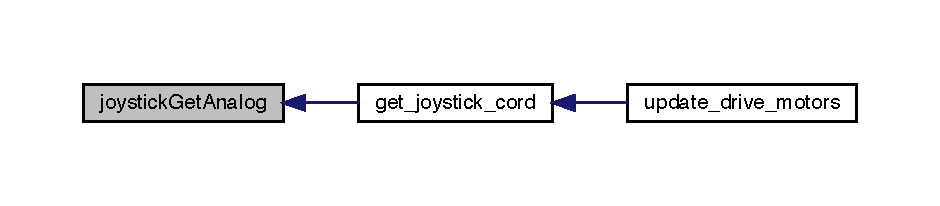
\includegraphics[width=350pt]{_a_p_i_8h_ad56fcec15d1a48deb8780bb0fc38be4d_icgraph}
\end{center}
\end{figure}
\mbox{\label{_a_p_i_8h_a792f1a80c62a63e764cf64aabf95db92}} 
\index{A\+P\+I.\+h@{A\+P\+I.\+h}!joystick\+Get\+Digital@{joystick\+Get\+Digital}}
\index{joystick\+Get\+Digital@{joystick\+Get\+Digital}!A\+P\+I.\+h@{A\+P\+I.\+h}}
\paragraph{joystick\+Get\+Digital()}
{\footnotesize\ttfamily bool joystick\+Get\+Digital (\begin{DoxyParamCaption}\item[{unsigned char}]{joystick,  }\item[{unsigned char}]{button\+Group,  }\item[{unsigned char}]{button }\end{DoxyParamCaption})}

Gets the value of a button on the V\+EX joystick. Returns true if that button is pressed, or false otherwise. If no joystick is connected to the requested slot, returns false.


\begin{DoxyParams}{Parameters}
{\em joystick} & the joystick slot to check \\
\hline
{\em button\+Group} & one of 5, 6, 7, or 8 to request that button as labelled on the joystick \\
\hline
{\em button} & one of J\+O\+Y\+\_\+\+UP, J\+O\+Y\+\_\+\+D\+O\+WN, J\+O\+Y\+\_\+\+L\+E\+FT, or J\+O\+Y\+\_\+\+R\+I\+G\+HT; requesting J\+O\+Y\+\_\+\+L\+E\+FT or J\+O\+Y\+\_\+\+R\+I\+G\+HT for groups 5 or 6 will cause an undefined value to be returned \\
\hline
\end{DoxyParams}


Referenced by \textbf{ button\+Get\+State()}, \textbf{ update\+\_\+claw()}, \textbf{ update\+\_\+control()}, \textbf{ update\+\_\+lifter()}, and \textbf{ update\+Intake()}.

Here is the caller graph for this function\+:\nopagebreak
\begin{figure}[H]
\begin{center}
\leavevmode
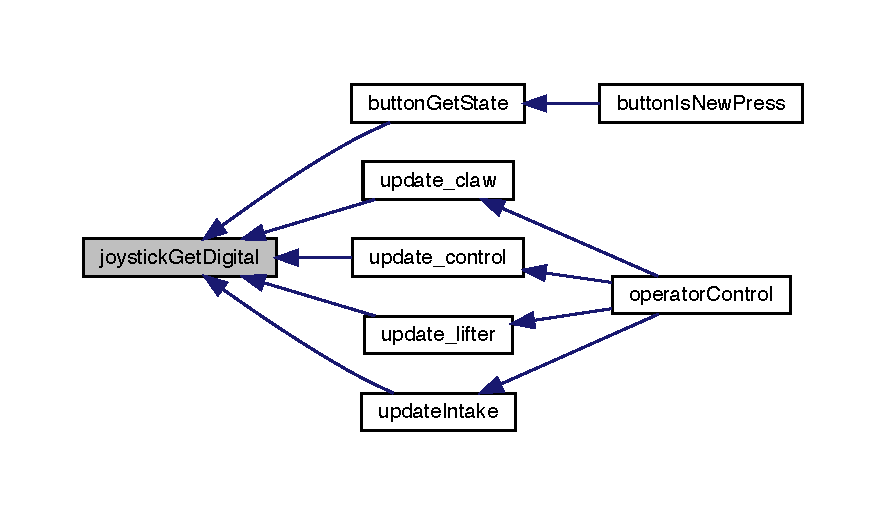
\includegraphics[width=350pt]{_a_p_i_8h_a792f1a80c62a63e764cf64aabf95db92_icgraph}
\end{center}
\end{figure}
\mbox{\label{_a_p_i_8h_a5fa1d119fe3e836b5519f97eae7a1272}} 
\index{A\+P\+I.\+h@{A\+P\+I.\+h}!lcd\+Clear@{lcd\+Clear}}
\index{lcd\+Clear@{lcd\+Clear}!A\+P\+I.\+h@{A\+P\+I.\+h}}
\paragraph{lcd\+Clear()}
{\footnotesize\ttfamily void lcd\+Clear (\begin{DoxyParamCaption}\item[{\textbf{ P\+R\+O\+S\+\_\+\+F\+I\+LE} $\ast$}]{lcd\+Port }\end{DoxyParamCaption})}

Clears the L\+CD screen on the specified port.

Printing to a line implicitly overwrites the contents, so clearing should only be required at startup.


\begin{DoxyParams}{Parameters}
{\em lcd\+Port} & the L\+CD to clear, either uart1 or uart2 \\
\hline
\end{DoxyParams}


Referenced by \textbf{ init\+\_\+main\+\_\+lcd()}, \textbf{ lcd\+\_\+clear()}, and \textbf{ log\+\_\+info()}.

Here is the caller graph for this function\+:\nopagebreak
\begin{figure}[H]
\begin{center}
\leavevmode
\includegraphics[width=350pt]{_a_p_i_8h_a5fa1d119fe3e836b5519f97eae7a1272_icgraph}
\end{center}
\end{figure}
\mbox{\label{_a_p_i_8h_a43dc11a67b697c0d32315ea5a9af85f9}} 
\index{A\+P\+I.\+h@{A\+P\+I.\+h}!lcd\+Init@{lcd\+Init}}
\index{lcd\+Init@{lcd\+Init}!A\+P\+I.\+h@{A\+P\+I.\+h}}
\paragraph{lcd\+Init()}
{\footnotesize\ttfamily void lcd\+Init (\begin{DoxyParamCaption}\item[{\textbf{ P\+R\+O\+S\+\_\+\+F\+I\+LE} $\ast$}]{lcd\+Port }\end{DoxyParamCaption})}

Initializes the L\+CD port, but does not change the text or settings.

If the L\+CD was not initialized before, the text currently on the screen will be undefined. The port will not be usable with standard serial port functions until the L\+CD is stopped.


\begin{DoxyParams}{Parameters}
{\em lcd\+Port} & the L\+CD to initialize, either uart1 or uart2 \\
\hline
\end{DoxyParams}


Referenced by \textbf{ init\+\_\+error()}, and \textbf{ init\+\_\+main\+\_\+lcd()}.

Here is the caller graph for this function\+:\nopagebreak
\begin{figure}[H]
\begin{center}
\leavevmode
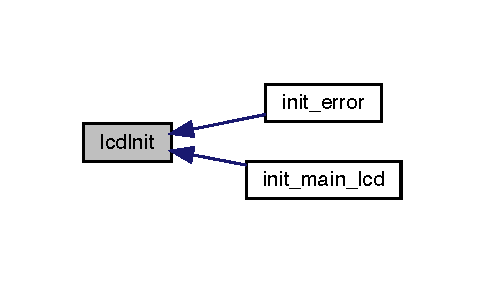
\includegraphics[width=232pt]{_a_p_i_8h_a43dc11a67b697c0d32315ea5a9af85f9_icgraph}
\end{center}
\end{figure}
\mbox{\label{_a_p_i_8h_a04541d90f60b1ccd3d036656673c972d}} 
\index{A\+P\+I.\+h@{A\+P\+I.\+h}!lcd\+Read\+Buttons@{lcd\+Read\+Buttons}}
\index{lcd\+Read\+Buttons@{lcd\+Read\+Buttons}!A\+P\+I.\+h@{A\+P\+I.\+h}}
\paragraph{lcd\+Read\+Buttons()}
{\footnotesize\ttfamily void unsigned char const char unsigned int lcd\+Read\+Buttons (\begin{DoxyParamCaption}\item[{\textbf{ P\+R\+O\+S\+\_\+\+F\+I\+LE} $\ast$}]{lcd\+Port }\end{DoxyParamCaption})}

Reads the user button status from the L\+CD display.

For example, if the left and right buttons are pushed, (1 $\vert$ 4) = 5 will be returned. 0 is returned if no buttons are pushed.


\begin{DoxyParams}{Parameters}
{\em lcd\+Port} & the L\+CD to poll, either uart1 or uart2 \\
\hline
\end{DoxyParams}
\begin{DoxyReturn}{Returns}
the buttons pressed as a bit mask 
\end{DoxyReturn}


Referenced by \textbf{ button\+Get\+State()}, and \textbf{ lcd\+\_\+get\+\_\+pressed\+\_\+buttons()}.

Here is the caller graph for this function\+:\nopagebreak
\begin{figure}[H]
\begin{center}
\leavevmode
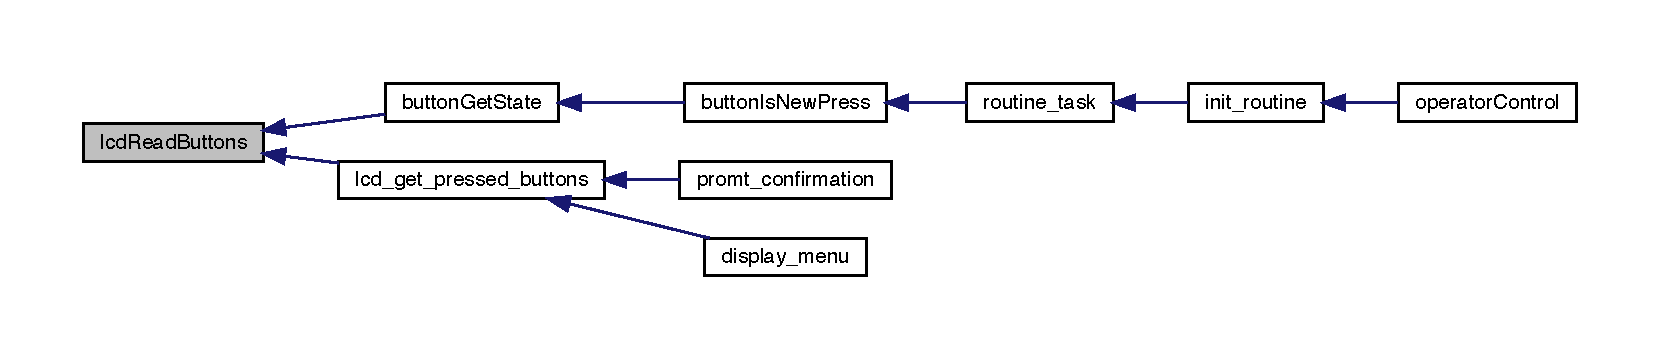
\includegraphics[width=350pt]{_a_p_i_8h_a04541d90f60b1ccd3d036656673c972d_icgraph}
\end{center}
\end{figure}
\mbox{\label{_a_p_i_8h_aab53a247d88151a6623c20fa1ea940b0}} 
\index{A\+P\+I.\+h@{A\+P\+I.\+h}!lcd\+Set\+Backlight@{lcd\+Set\+Backlight}}
\index{lcd\+Set\+Backlight@{lcd\+Set\+Backlight}!A\+P\+I.\+h@{A\+P\+I.\+h}}
\paragraph{lcd\+Set\+Backlight()}
{\footnotesize\ttfamily void lcd\+Set\+Backlight (\begin{DoxyParamCaption}\item[{\textbf{ P\+R\+O\+S\+\_\+\+F\+I\+LE} $\ast$}]{lcd\+Port,  }\item[{bool}]{backlight }\end{DoxyParamCaption})}

Sets the specified L\+CD backlight to be on or off.

Turning it off will save power but may make it more difficult to read in dim conditions.


\begin{DoxyParams}{Parameters}
{\em lcd\+Port} & the L\+CD to adjust, either uart1 or uart2 \\
\hline
{\em backlight} & true to turn the backlight on, or false to turn it off \\
\hline
\end{DoxyParams}


Referenced by \textbf{ lcd\+\_\+set\+\_\+backlight()}, and \textbf{ log\+\_\+info()}.

Here is the caller graph for this function\+:\nopagebreak
\begin{figure}[H]
\begin{center}
\leavevmode
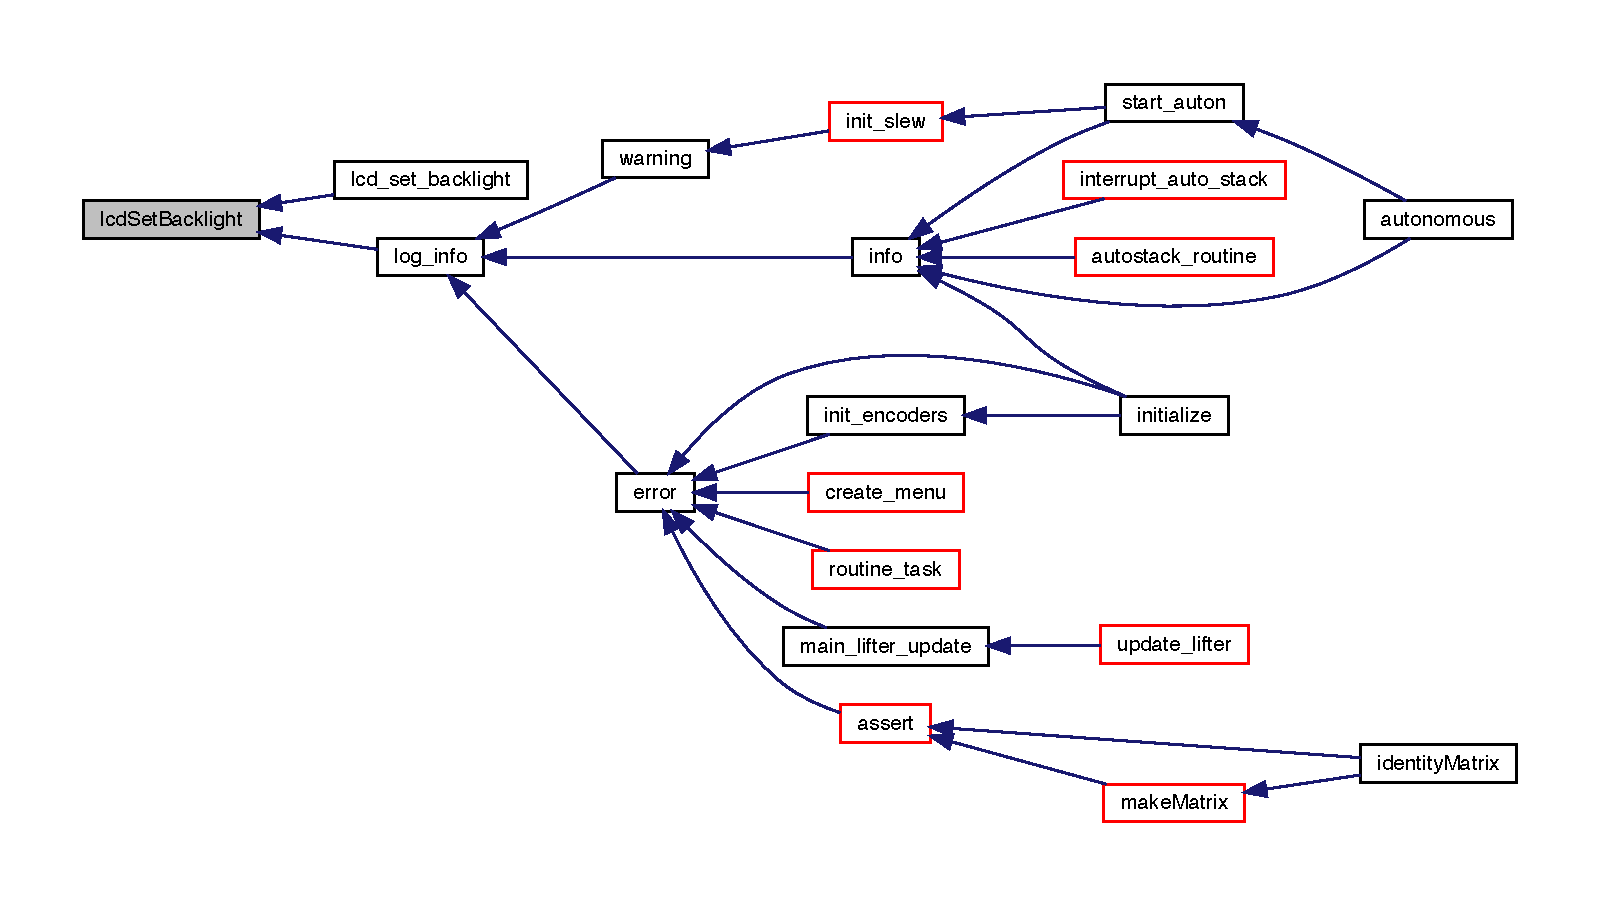
\includegraphics[width=350pt]{_a_p_i_8h_aab53a247d88151a6623c20fa1ea940b0_icgraph}
\end{center}
\end{figure}
\mbox{\label{_a_p_i_8h_a5555228be96449af952aed5bcabb6d8d}} 
\index{A\+P\+I.\+h@{A\+P\+I.\+h}!lcd\+Set\+Text@{lcd\+Set\+Text}}
\index{lcd\+Set\+Text@{lcd\+Set\+Text}!A\+P\+I.\+h@{A\+P\+I.\+h}}
\paragraph{lcd\+Set\+Text()}
{\footnotesize\ttfamily void lcd\+Set\+Text (\begin{DoxyParamCaption}\item[{\textbf{ P\+R\+O\+S\+\_\+\+F\+I\+LE} $\ast$}]{lcd\+Port,  }\item[{unsigned char}]{line,  }\item[{const char $\ast$}]{buffer }\end{DoxyParamCaption})}

Prints the string buffer to the attached L\+CD.

The output string will be truncated as necessary to fit on the L\+CD screen, 16 characters wide. This function, like \doxyref{fprint()}{p.}{_a_p_i_8h_a874987bcf339f25df0bdbc24f27a03db}, is much, much faster than a formatted routine such as lcd\+Print() and consumes less memory.


\begin{DoxyParams}{Parameters}
{\em lcd\+Port} & the L\+CD to write, either uart1 or uart2 \\
\hline
{\em line} & the L\+CD line to write, either 1 or 2 \\
\hline
{\em buffer} & the string to write \\
\hline
\end{DoxyParams}


Referenced by \textbf{ lcd\+\_\+print()}.

Here is the caller graph for this function\+:\nopagebreak
\begin{figure}[H]
\begin{center}
\leavevmode
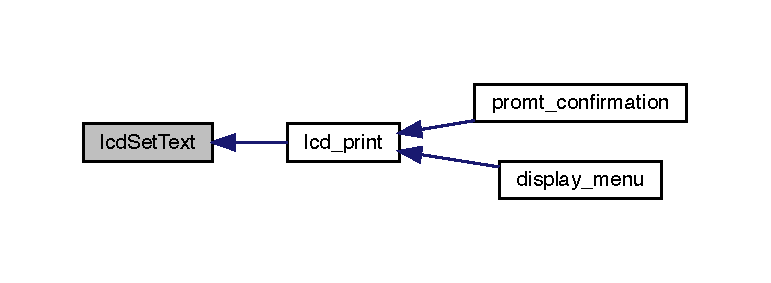
\includegraphics[width=350pt]{_a_p_i_8h_a5555228be96449af952aed5bcabb6d8d_icgraph}
\end{center}
\end{figure}
\mbox{\label{_a_p_i_8h_acf0a8389bc6078e4c40c3d59af814cb7}} 
\index{A\+P\+I.\+h@{A\+P\+I.\+h}!lcd\+Shutdown@{lcd\+Shutdown}}
\index{lcd\+Shutdown@{lcd\+Shutdown}!A\+P\+I.\+h@{A\+P\+I.\+h}}
\paragraph{lcd\+Shutdown()}
{\footnotesize\ttfamily void lcd\+Shutdown (\begin{DoxyParamCaption}\item[{\textbf{ P\+R\+O\+S\+\_\+\+F\+I\+LE} $\ast$}]{lcd\+Port }\end{DoxyParamCaption})}

Shut down the specified L\+CD port.


\begin{DoxyParams}{Parameters}
{\em lcd\+Port} & the L\+CD to stop, either uart1 or uart2 \\
\hline
\end{DoxyParams}
\mbox{\label{_a_p_i_8h_a8b24cbb7c3486e1bfa05c86db83ecb01}} 
\index{A\+P\+I.\+h@{A\+P\+I.\+h}!micros@{micros}}
\index{micros@{micros}!A\+P\+I.\+h@{A\+P\+I.\+h}}
\paragraph{micros()}
{\footnotesize\ttfamily unsigned long micros (\begin{DoxyParamCaption}{ }\end{DoxyParamCaption})}

Returns the number of microseconds since Cortex power-\/up. There are 10$^\wedge$6 microseconds in a second, so as a 32-\/bit integer, this will overflow and wrap back to zero every two hours or so.

This function is Wiring-\/compatible.

\begin{DoxyReturn}{Returns}
the number of microseconds since the Cortex was turned on or the last overflow 
\end{DoxyReturn}
\mbox{\label{_a_p_i_8h_a6ff7f2532a22366f0013bc41397129fd}} 
\index{A\+P\+I.\+h@{A\+P\+I.\+h}!millis@{millis}}
\index{millis@{millis}!A\+P\+I.\+h@{A\+P\+I.\+h}}
\paragraph{millis()}
{\footnotesize\ttfamily unsigned long millis (\begin{DoxyParamCaption}{ }\end{DoxyParamCaption})}

Returns the number of milliseconds since Cortex power-\/up. There are 1000 milliseconds in a second, so as a 32-\/bit integer, this will not overflow for 50 days.

This function is Wiring-\/compatible.

\begin{DoxyReturn}{Returns}
the number of milliseconds since the Cortex was turned on 
\end{DoxyReturn}


Referenced by \textbf{ calculate\+\_\+accelerometer\+\_\+odemetry()}, \textbf{ init\+\_\+localization()}, and \textbf{ update\+\_\+position()}.

Here is the caller graph for this function\+:\nopagebreak
\begin{figure}[H]
\begin{center}
\leavevmode
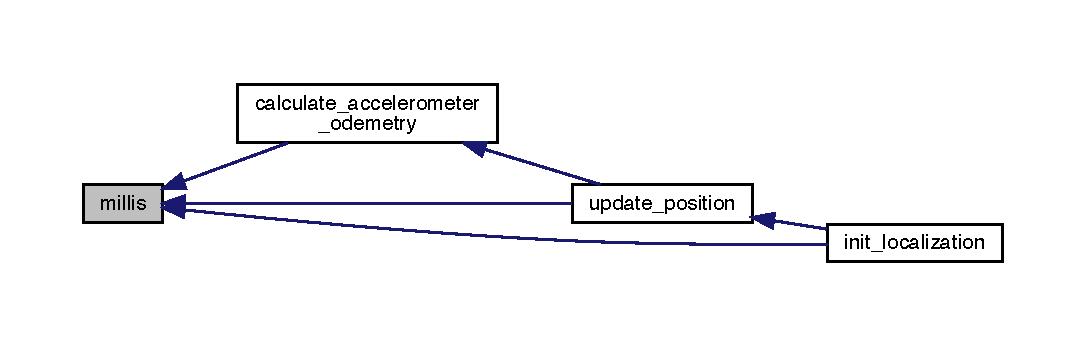
\includegraphics[width=350pt]{_a_p_i_8h_a6ff7f2532a22366f0013bc41397129fd_icgraph}
\end{center}
\end{figure}
\mbox{\label{_a_p_i_8h_a4805c8fd29f9221d28ed2e673c06e6c4}} 
\index{A\+P\+I.\+h@{A\+P\+I.\+h}!motor\+Get@{motor\+Get}}
\index{motor\+Get@{motor\+Get}!A\+P\+I.\+h@{A\+P\+I.\+h}}
\paragraph{motor\+Get()}
{\footnotesize\ttfamily int motor\+Get (\begin{DoxyParamCaption}\item[{unsigned char}]{channel }\end{DoxyParamCaption})}

Gets the last set speed of the specified motor channel.

This speed may have been set by any task or the P\+R\+OS kernel itself. This is not guaranteed to be the speed that the motor is actually running at, or even the speed currently being sent to the motor, due to latency in the Motor Controller 29 protocol and physical loading. To measure actual motor shaft revolution speed, attach a V\+EX Integrated Motor Encoder or V\+EX Quadrature Encoder and use the velocity functions associated with each.


\begin{DoxyParams}{Parameters}
{\em channel} & the motor channel to fetch from 1-\/10 \\
\hline
\end{DoxyParams}
\begin{DoxyReturn}{Returns}
the speed last sent to this channel; -\/127 is full reverse and 127 is full forward, with 0 being off 
\end{DoxyReturn}
\mbox{\label{_a_p_i_8h_a03c5b04b472d024281f62d7af8854a8e}} 
\index{A\+P\+I.\+h@{A\+P\+I.\+h}!motor\+Set@{motor\+Set}}
\index{motor\+Set@{motor\+Set}!A\+P\+I.\+h@{A\+P\+I.\+h}}
\paragraph{motor\+Set()}
{\footnotesize\ttfamily void motor\+Set (\begin{DoxyParamCaption}\item[{unsigned char}]{channel,  }\item[{int}]{speed }\end{DoxyParamCaption})}

Sets the speed of the specified motor channel.

Do not use \doxyref{motor\+Set()}{p.}{_a_p_i_8h_a03c5b04b472d024281f62d7af8854a8e} with the same channel argument from two different tasks. It is safe to use \doxyref{motor\+Set()}{p.}{_a_p_i_8h_a03c5b04b472d024281f62d7af8854a8e} with different channel arguments from different tasks.


\begin{DoxyParams}{Parameters}
{\em channel} & the motor channel to modify from 1-\/10 \\
\hline
{\em speed} & the new signed speed; -\/127 is full reverse and 127 is full forward, with 0 being off \\
\hline
\end{DoxyParams}


Referenced by \textbf{ set\+\_\+motor\+\_\+immediate()}, and \textbf{ update\+Motors()}.

Here is the caller graph for this function\+:\nopagebreak
\begin{figure}[H]
\begin{center}
\leavevmode
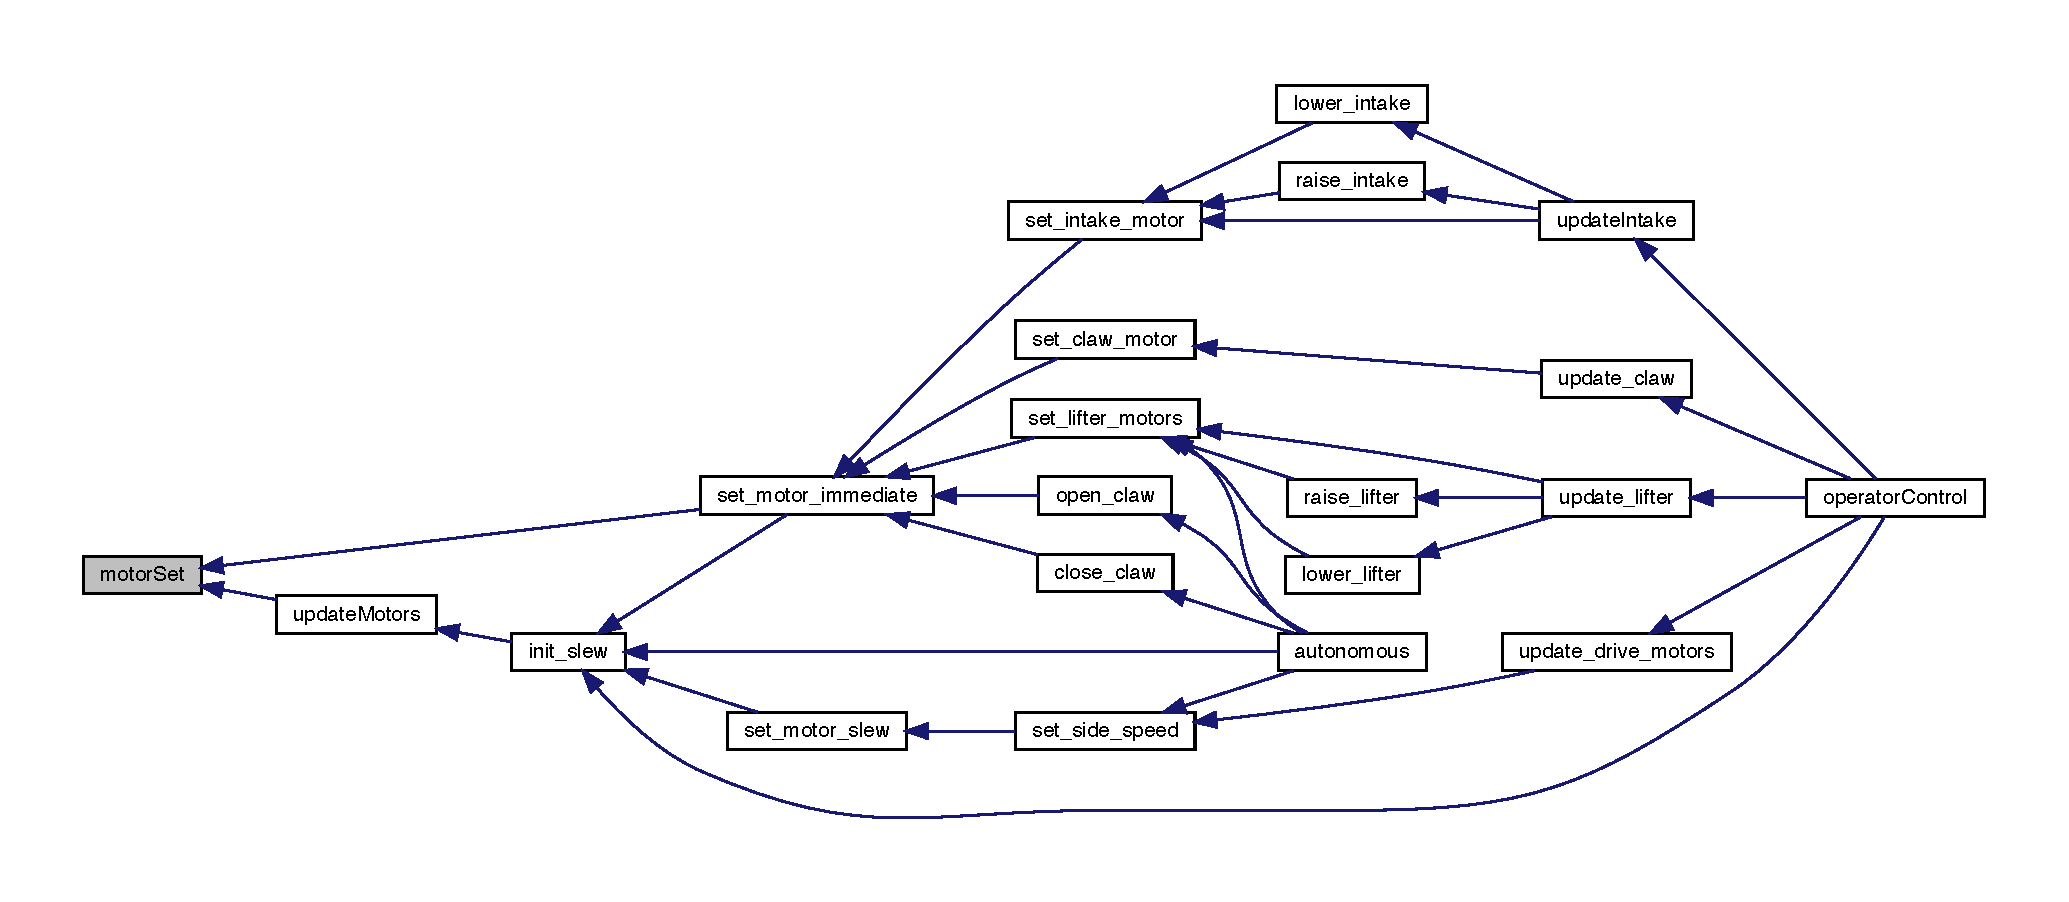
\includegraphics[width=350pt]{_a_p_i_8h_a03c5b04b472d024281f62d7af8854a8e_icgraph}
\end{center}
\end{figure}
\mbox{\label{_a_p_i_8h_a339844ebc35f48a14945b73edaeca498}} 
\index{A\+P\+I.\+h@{A\+P\+I.\+h}!motor\+Stop@{motor\+Stop}}
\index{motor\+Stop@{motor\+Stop}!A\+P\+I.\+h@{A\+P\+I.\+h}}
\paragraph{motor\+Stop()}
{\footnotesize\ttfamily void motor\+Stop (\begin{DoxyParamCaption}\item[{unsigned char}]{channel }\end{DoxyParamCaption})}

Stops the motor on the specified channel, equivalent to calling \doxyref{motor\+Set()}{p.}{_a_p_i_8h_a03c5b04b472d024281f62d7af8854a8e} with an argument of zero.

This performs a coasting stop, not an active brake. Since motor\+Stop is similar to motor\+Set(0), see the note for \doxyref{motor\+Set()}{p.}{_a_p_i_8h_a03c5b04b472d024281f62d7af8854a8e} about use from multiple tasks.


\begin{DoxyParams}{Parameters}
{\em channel} & the motor channel to stop from 1-\/10 \\
\hline
\end{DoxyParams}
\mbox{\label{_a_p_i_8h_a8966c541f3e9565aea1289f0d2f2cf43}} 
\index{A\+P\+I.\+h@{A\+P\+I.\+h}!motor\+Stop\+All@{motor\+Stop\+All}}
\index{motor\+Stop\+All@{motor\+Stop\+All}!A\+P\+I.\+h@{A\+P\+I.\+h}}
\paragraph{motor\+Stop\+All()}
{\footnotesize\ttfamily void motor\+Stop\+All (\begin{DoxyParamCaption}{ }\end{DoxyParamCaption})}

Stops all motors; significantly faster than looping through all motor ports and calling motor\+Set(channel, 0) on each one. 

Referenced by \textbf{ init\+\_\+slew()}.

Here is the caller graph for this function\+:\nopagebreak
\begin{figure}[H]
\begin{center}
\leavevmode
\includegraphics[width=350pt]{_a_p_i_8h_a8966c541f3e9565aea1289f0d2f2cf43_icgraph}
\end{center}
\end{figure}
\mbox{\label{_a_p_i_8h_aecd027ce8f8b52a765735e9eb5b202b3}} 
\index{A\+P\+I.\+h@{A\+P\+I.\+h}!mutex\+Create@{mutex\+Create}}
\index{mutex\+Create@{mutex\+Create}!A\+P\+I.\+h@{A\+P\+I.\+h}}
\paragraph{mutex\+Create()}
{\footnotesize\ttfamily \textbf{ Mutex} mutex\+Create (\begin{DoxyParamCaption}{ }\end{DoxyParamCaption})}

Creates a mutex intended to allow only one task to use a resource at a time. For signalling and synchronization, try using semaphores.

Mutexes created using this function can be accessed using the \doxyref{mutex\+Take()}{p.}{_a_p_i_8h_a8b51124628d2a7741738d48551d1e8ee} and \doxyref{mutex\+Give()}{p.}{_a_p_i_8h_afe171a08d22de18fc2ab604b2364959f} functions. The semaphore functions must not be used on objects of this type.

This type of object uses a priority inheritance mechanism so a task \textquotesingle{}taking\textquotesingle{} a mutex M\+U\+ST A\+L\+W\+A\+YS \textquotesingle{}give\textquotesingle{} the mutex back once the mutex is no longer required.

\begin{DoxyReturn}{Returns}
a handle to the created mutex 
\end{DoxyReturn}


Referenced by \textbf{ init\+\_\+slew()}.

Here is the caller graph for this function\+:\nopagebreak
\begin{figure}[H]
\begin{center}
\leavevmode
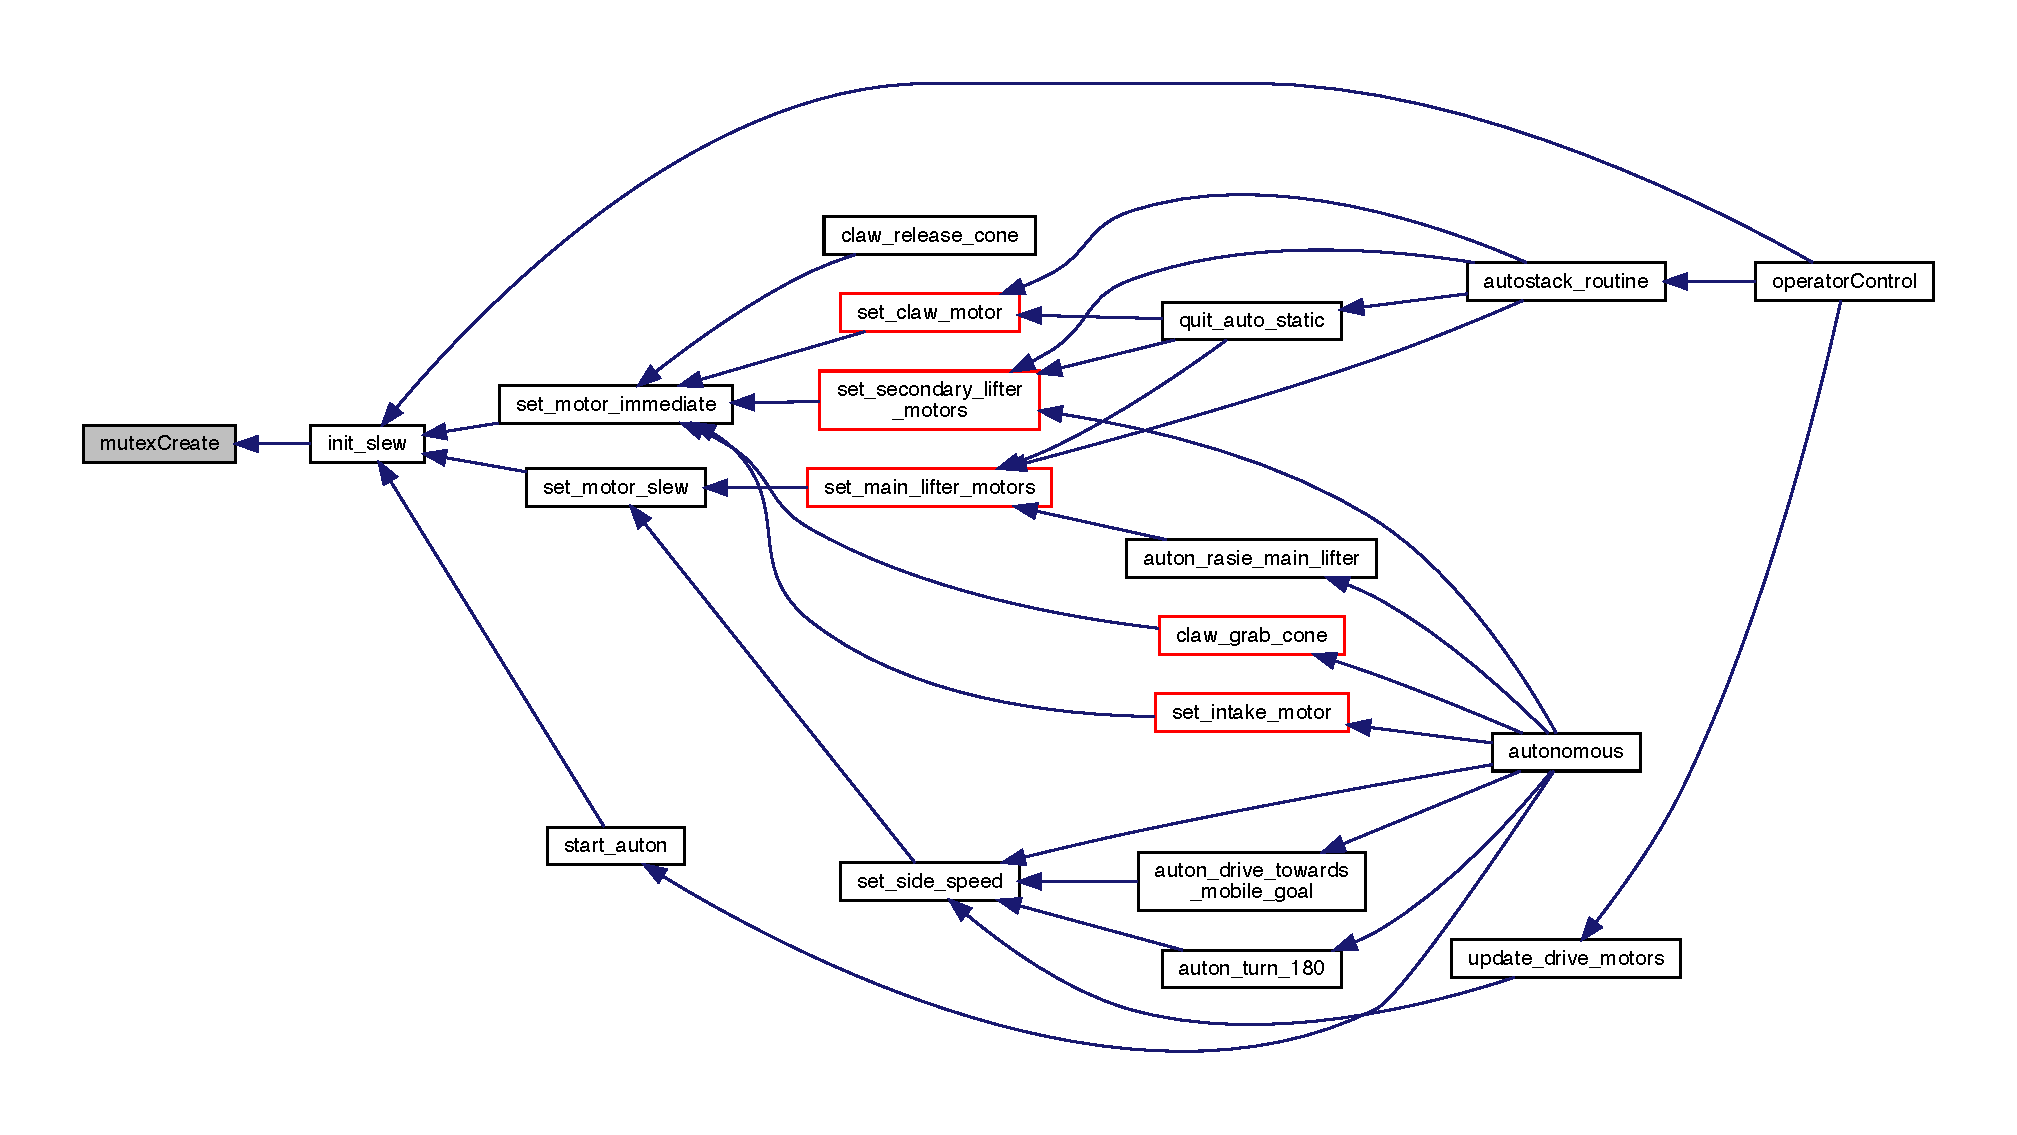
\includegraphics[width=350pt]{_a_p_i_8h_aecd027ce8f8b52a765735e9eb5b202b3_icgraph}
\end{center}
\end{figure}
\mbox{\label{_a_p_i_8h_a247598f8083a3ce6c39317d279f631cf}} 
\index{A\+P\+I.\+h@{A\+P\+I.\+h}!mutex\+Delete@{mutex\+Delete}}
\index{mutex\+Delete@{mutex\+Delete}!A\+P\+I.\+h@{A\+P\+I.\+h}}
\paragraph{mutex\+Delete()}
{\footnotesize\ttfamily void mutex\+Delete (\begin{DoxyParamCaption}\item[{\textbf{ Mutex}}]{mutex }\end{DoxyParamCaption})}

Deletes the specified mutex. This function can be dangerous; deleting semaphores being waited on by a task may cause deadlock or a crash.


\begin{DoxyParams}{Parameters}
{\em mutex} & the mutex to destroy \\
\hline
\end{DoxyParams}
\mbox{\label{_a_p_i_8h_afe171a08d22de18fc2ab604b2364959f}} 
\index{A\+P\+I.\+h@{A\+P\+I.\+h}!mutex\+Give@{mutex\+Give}}
\index{mutex\+Give@{mutex\+Give}!A\+P\+I.\+h@{A\+P\+I.\+h}}
\paragraph{mutex\+Give()}
{\footnotesize\ttfamily bool mutex\+Give (\begin{DoxyParamCaption}\item[{\textbf{ Mutex}}]{mutex }\end{DoxyParamCaption})}

Relinquishes a mutex so that other tasks can use the resource it guards. The mutex must be held by the current task using a corresponding call to mutex\+Take.


\begin{DoxyParams}{Parameters}
{\em mutex} & the mutex to release \\
\hline
\end{DoxyParams}
\begin{DoxyReturn}{Returns}
true if the mutex was released, or false if the mutex was not already held 
\end{DoxyReturn}


Referenced by \textbf{ set\+\_\+motor\+\_\+immediate()}, \textbf{ set\+\_\+motor\+\_\+slew()}, and \textbf{ update\+Motors()}.

Here is the caller graph for this function\+:\nopagebreak
\begin{figure}[H]
\begin{center}
\leavevmode
\includegraphics[width=350pt]{_a_p_i_8h_afe171a08d22de18fc2ab604b2364959f_icgraph}
\end{center}
\end{figure}
\mbox{\label{_a_p_i_8h_a8b51124628d2a7741738d48551d1e8ee}} 
\index{A\+P\+I.\+h@{A\+P\+I.\+h}!mutex\+Take@{mutex\+Take}}
\index{mutex\+Take@{mutex\+Take}!A\+P\+I.\+h@{A\+P\+I.\+h}}
\paragraph{mutex\+Take()}
{\footnotesize\ttfamily bool mutex\+Take (\begin{DoxyParamCaption}\item[{\textbf{ Mutex}}]{mutex,  }\item[{const unsigned long}]{block\+Time }\end{DoxyParamCaption})}

Requests a mutex so that other tasks cannot simultaneously use the resource it guards. The mutex must not already be held by the current task. If another task already holds the mutex, the function will wait for the mutex to be released. Other tasks can run during this time.


\begin{DoxyParams}{Parameters}
{\em mutex} & the mutex to request \\
\hline
{\em block\+Time} & the maximum time to wait for the mutex to be available, where -\/1 specifies an infinite timeout \\
\hline
\end{DoxyParams}
\begin{DoxyReturn}{Returns}
true if the mutex was successfully taken, or false if the timeout expired 
\end{DoxyReturn}


Referenced by \textbf{ set\+\_\+motor\+\_\+immediate()}, \textbf{ set\+\_\+motor\+\_\+slew()}, and \textbf{ update\+Motors()}.

Here is the caller graph for this function\+:\nopagebreak
\begin{figure}[H]
\begin{center}
\leavevmode
\includegraphics[width=350pt]{_a_p_i_8h_a8b51124628d2a7741738d48551d1e8ee_icgraph}
\end{center}
\end{figure}
\mbox{\label{_a_p_i_8h_a1875409d12eee562555bda94cad7f973}} 
\index{A\+P\+I.\+h@{A\+P\+I.\+h}!pin\+Mode@{pin\+Mode}}
\index{pin\+Mode@{pin\+Mode}!A\+P\+I.\+h@{A\+P\+I.\+h}}
\paragraph{pin\+Mode()}
{\footnotesize\ttfamily void pin\+Mode (\begin{DoxyParamCaption}\item[{unsigned char}]{pin,  }\item[{unsigned char}]{mode }\end{DoxyParamCaption})}

Configures the pin as an input or output with a variety of settings.

Do note that I\+N\+P\+UT by default turns on the pull-\/up resistor, as most V\+EX sensors are open-\/drain active low. It should not be a big deal for most push-\/pull sources. This function is Wiring-\/compatible.


\begin{DoxyParams}{Parameters}
{\em pin} & the pin to modify from 1-\/26 \\
\hline
{\em mode} & one of I\+N\+P\+UT, I\+N\+P\+U\+T\+\_\+\+A\+N\+A\+L\+OG, I\+N\+P\+U\+T\+\_\+\+F\+L\+O\+A\+T\+I\+NG, O\+U\+T\+P\+UT, or O\+U\+T\+P\+U\+T\+\_\+\+OD \\
\hline
\end{DoxyParams}
\mbox{\label{_a_p_i_8h_a91ac9eacbf0930cd5f26bc12b90b9efd}} 
\index{A\+P\+I.\+h@{A\+P\+I.\+h}!power\+Level\+Backup@{power\+Level\+Backup}}
\index{power\+Level\+Backup@{power\+Level\+Backup}!A\+P\+I.\+h@{A\+P\+I.\+h}}
\paragraph{power\+Level\+Backup()}
{\footnotesize\ttfamily unsigned int power\+Level\+Backup (\begin{DoxyParamCaption}{ }\end{DoxyParamCaption})}

Returns the backup battery voltage in millivolts.

If no backup battery is connected, returns 0. 

Referenced by \textbf{ backup\+\_\+battery\+\_\+voltage()}.

Here is the caller graph for this function\+:\nopagebreak
\begin{figure}[H]
\begin{center}
\leavevmode
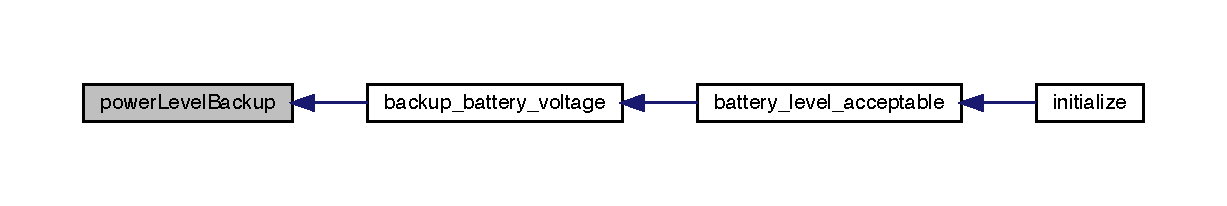
\includegraphics[width=350pt]{_a_p_i_8h_a91ac9eacbf0930cd5f26bc12b90b9efd_icgraph}
\end{center}
\end{figure}
\mbox{\label{_a_p_i_8h_aeb5efefae0d6fa559dae5a7e5a77c956}} 
\index{A\+P\+I.\+h@{A\+P\+I.\+h}!power\+Level\+Main@{power\+Level\+Main}}
\index{power\+Level\+Main@{power\+Level\+Main}!A\+P\+I.\+h@{A\+P\+I.\+h}}
\paragraph{power\+Level\+Main()}
{\footnotesize\ttfamily unsigned int power\+Level\+Main (\begin{DoxyParamCaption}{ }\end{DoxyParamCaption})}

Returns the main battery voltage in millivolts.

In rare circumstances, this method might return 0. Check the output value for reasonability before blindly blasting the user. 

Referenced by \textbf{ main\+\_\+battery\+\_\+voltage()}.

Here is the caller graph for this function\+:\nopagebreak
\begin{figure}[H]
\begin{center}
\leavevmode
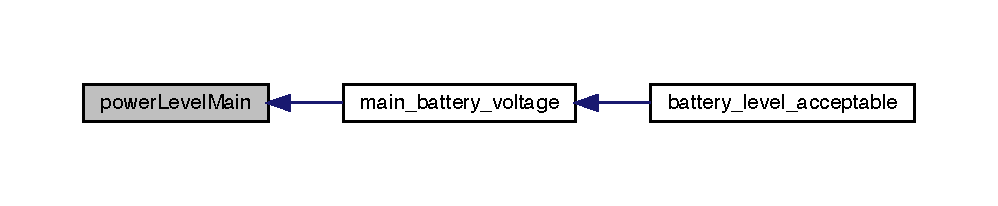
\includegraphics[width=350pt]{_a_p_i_8h_aeb5efefae0d6fa559dae5a7e5a77c956_icgraph}
\end{center}
\end{figure}
\mbox{\label{_a_p_i_8h_ae2dd7886efd463e815dadf10eb54777e}} 
\index{A\+P\+I.\+h@{A\+P\+I.\+h}!print@{print}}
\index{print@{print}!A\+P\+I.\+h@{A\+P\+I.\+h}}
\paragraph{print()}
{\footnotesize\ttfamily void print (\begin{DoxyParamCaption}\item[{const char $\ast$}]{string }\end{DoxyParamCaption})}

Prints the simple string to the debug terminal without formatting.

This method is much, much faster than \doxyref{printf()}{p.}{_a_p_i_8h_a403c82418e475fa4a8273719e6a7f3e6}.


\begin{DoxyParams}{Parameters}
{\em string} & the string to write \\
\hline
\end{DoxyParams}
\mbox{\label{_a_p_i_8h_a403c82418e475fa4a8273719e6a7f3e6}} 
\index{A\+P\+I.\+h@{A\+P\+I.\+h}!printf@{printf}}
\index{printf@{printf}!A\+P\+I.\+h@{A\+P\+I.\+h}}
\paragraph{printf()}
{\footnotesize\ttfamily int printf (\begin{DoxyParamCaption}\item[{const char $\ast$}]{format\+String,  }\item[{}]{... }\end{DoxyParamCaption})}

Prints the formatted string to the debug stream (the PC terminal).


\begin{DoxyParams}{Parameters}
{\em format\+String} & the format string as specified in \doxyref{fprintf()}{p.}{_a_p_i_8h_ab9989f4619e4d3ccb13ed4c36d5f787a} \\
\hline
\end{DoxyParams}
\begin{DoxyReturn}{Returns}
the number of characters written 
\end{DoxyReturn}


Referenced by \textbf{ autonomous()}, \textbf{ calculate\+\_\+accelerometer\+\_\+odemetry()}, \textbf{ debug()}, \textbf{ info()}, \textbf{ initialize()}, \textbf{ lcd\+\_\+assert()}, \textbf{ log\+\_\+info()}, and \textbf{ print\+Matrix()}.

Here is the caller graph for this function\+:\nopagebreak
\begin{figure}[H]
\begin{center}
\leavevmode
\includegraphics[width=350pt]{_a_p_i_8h_a403c82418e475fa4a8273719e6a7f3e6_icgraph}
\end{center}
\end{figure}
\mbox{\label{_a_p_i_8h_a6c600555ec9aefb4c01fdb960ecc2809}} 
\index{A\+P\+I.\+h@{A\+P\+I.\+h}!putchar@{putchar}}
\index{putchar@{putchar}!A\+P\+I.\+h@{A\+P\+I.\+h}}
\paragraph{putchar()}
{\footnotesize\ttfamily int putchar (\begin{DoxyParamCaption}\item[{int}]{value }\end{DoxyParamCaption})}

Writes one character to \char`\"{}stdout\char`\"{}, which is the PC debug terminal, and returns the input value.

When using a wireless connection, one may need to press the spacebar before the input is visible on the terminal.


\begin{DoxyParams}{Parameters}
{\em value} & the character to write (a value of type \char`\"{}char\char`\"{} can be used) \\
\hline
\end{DoxyParams}
\begin{DoxyReturn}{Returns}
the character written 
\end{DoxyReturn}
\mbox{\label{_a_p_i_8h_af17f2f3fda696ddc3b7c1bac995edaf8}} 
\index{A\+P\+I.\+h@{A\+P\+I.\+h}!puts@{puts}}
\index{puts@{puts}!A\+P\+I.\+h@{A\+P\+I.\+h}}
\paragraph{puts()}
{\footnotesize\ttfamily int puts (\begin{DoxyParamCaption}\item[{const char $\ast$}]{string }\end{DoxyParamCaption})}

Behaves the same as the \char`\"{}print\char`\"{} function, and appends a trailing newline (\char`\"{}\textbackslash{}n\char`\"{}).


\begin{DoxyParams}{Parameters}
{\em string} & the string to write \\
\hline
\end{DoxyParams}
\begin{DoxyReturn}{Returns}
the number of characters written, excluding the new line 
\end{DoxyReturn}
\mbox{\label{_a_p_i_8h_a4461acf29574576dda6a3316117f85a9}} 
\index{A\+P\+I.\+h@{A\+P\+I.\+h}!semaphore\+Create@{semaphore\+Create}}
\index{semaphore\+Create@{semaphore\+Create}!A\+P\+I.\+h@{A\+P\+I.\+h}}
\paragraph{semaphore\+Create()}
{\footnotesize\ttfamily \textbf{ Semaphore} semaphore\+Create (\begin{DoxyParamCaption}{ }\end{DoxyParamCaption})}

Creates a semaphore intended for synchronizing tasks. To prevent some critical code from simultaneously modifying a shared resource, use mutexes instead.

Semaphores created using this function can be accessed using the \doxyref{semaphore\+Take()}{p.}{_a_p_i_8h_a7520baa9cf5c9ec2f43925b098e7b46a} and \doxyref{semaphore\+Give()}{p.}{_a_p_i_8h_a9e5b0b6d5da138b4d5a077237894f96e} functions. The mutex functions must not be used on objects of this type.

This type of object does not need to have balanced take and give calls, so priority inheritance is not used. Semaphores can be signalled by an interrupt routine.

\begin{DoxyReturn}{Returns}
a handle to the created semaphore 
\end{DoxyReturn}
\mbox{\label{_a_p_i_8h_af27ba79dc102f914d31a3c20136b1cd9}} 
\index{A\+P\+I.\+h@{A\+P\+I.\+h}!semaphore\+Delete@{semaphore\+Delete}}
\index{semaphore\+Delete@{semaphore\+Delete}!A\+P\+I.\+h@{A\+P\+I.\+h}}
\paragraph{semaphore\+Delete()}
{\footnotesize\ttfamily void semaphore\+Delete (\begin{DoxyParamCaption}\item[{\textbf{ Semaphore}}]{semaphore }\end{DoxyParamCaption})}

Deletes the specified semaphore. This function can be dangerous; deleting semaphores being waited on by a task may cause deadlock or a crash.


\begin{DoxyParams}{Parameters}
{\em semaphore} & the semaphore to destroy \\
\hline
\end{DoxyParams}
\mbox{\label{_a_p_i_8h_a9e5b0b6d5da138b4d5a077237894f96e}} 
\index{A\+P\+I.\+h@{A\+P\+I.\+h}!semaphore\+Give@{semaphore\+Give}}
\index{semaphore\+Give@{semaphore\+Give}!A\+P\+I.\+h@{A\+P\+I.\+h}}
\paragraph{semaphore\+Give()}
{\footnotesize\ttfamily bool semaphore\+Give (\begin{DoxyParamCaption}\item[{\textbf{ Semaphore}}]{semaphore }\end{DoxyParamCaption})}

Signals a semaphore. Tasks waiting for a signal using \doxyref{semaphore\+Take()}{p.}{_a_p_i_8h_a7520baa9cf5c9ec2f43925b098e7b46a} will be unblocked by this call and can continue execution.

Slow processes can give semaphores when ready, and fast processes waiting to take the semaphore will continue at that point.


\begin{DoxyParams}{Parameters}
{\em semaphore} & the semaphore to signal \\
\hline
\end{DoxyParams}
\begin{DoxyReturn}{Returns}
true if the semaphore was successfully given, or false if the semaphore was not taken since the last give 
\end{DoxyReturn}
\mbox{\label{_a_p_i_8h_a7520baa9cf5c9ec2f43925b098e7b46a}} 
\index{A\+P\+I.\+h@{A\+P\+I.\+h}!semaphore\+Take@{semaphore\+Take}}
\index{semaphore\+Take@{semaphore\+Take}!A\+P\+I.\+h@{A\+P\+I.\+h}}
\paragraph{semaphore\+Take()}
{\footnotesize\ttfamily bool semaphore\+Take (\begin{DoxyParamCaption}\item[{\textbf{ Semaphore}}]{semaphore,  }\item[{const unsigned long}]{block\+Time }\end{DoxyParamCaption})}

Waits on a semaphore. If the semaphore is already in the \char`\"{}taken\char`\"{} state, the current task will wait for the semaphore to be signaled. Other tasks can run during this time.


\begin{DoxyParams}{Parameters}
{\em semaphore} & the semaphore to wait \\
\hline
{\em block\+Time} & the maximum time to wait for the semaphore to be given, where -\/1 specifies an infinite timeout \\
\hline
\end{DoxyParams}
\begin{DoxyReturn}{Returns}
true if the semaphore was successfully taken, or false if the timeout expired 
\end{DoxyReturn}
\mbox{\label{_a_p_i_8h_a22269cefc22e487f7acdcc4737d58c4a}} 
\index{A\+P\+I.\+h@{A\+P\+I.\+h}!set\+Team\+Name@{set\+Team\+Name}}
\index{set\+Team\+Name@{set\+Team\+Name}!A\+P\+I.\+h@{A\+P\+I.\+h}}
\paragraph{set\+Team\+Name()}
{\footnotesize\ttfamily void set\+Team\+Name (\begin{DoxyParamCaption}\item[{const char $\ast$}]{name }\end{DoxyParamCaption})}

Sets the team name displayed to the V\+EX field control and V\+EX Firmware Upgrade.


\begin{DoxyParams}{Parameters}
{\em name} & a string containing the team name; only the first eight characters will be shown \\
\hline
\end{DoxyParams}


Referenced by \textbf{ initialize()}.

Here is the caller graph for this function\+:\nopagebreak
\begin{figure}[H]
\begin{center}
\leavevmode
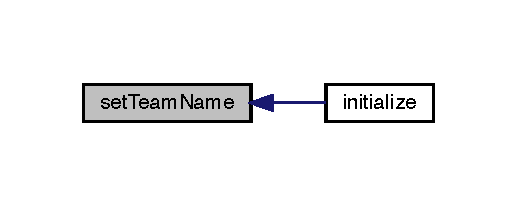
\includegraphics[width=248pt]{_a_p_i_8h_a22269cefc22e487f7acdcc4737d58c4a_icgraph}
\end{center}
\end{figure}
\mbox{\label{_a_p_i_8h_ada81026ae730d990159aab26c302a3ad}} 
\index{A\+P\+I.\+h@{A\+P\+I.\+h}!snprintf@{snprintf}}
\index{snprintf@{snprintf}!A\+P\+I.\+h@{A\+P\+I.\+h}}
\paragraph{snprintf()}
{\footnotesize\ttfamily int snprintf (\begin{DoxyParamCaption}\item[{char $\ast$}]{buffer,  }\item[{size\+\_\+t}]{limit,  }\item[{const char $\ast$}]{format\+String,  }\item[{}]{... }\end{DoxyParamCaption})}

Prints the formatted string to the string buffer with the specified length limit.

The length limit, as per the C standard, includes the trailing null character, so an argument of 256 will cause a maximum of 255 non-\/null characters to be printed, and one null terminator in all cases.


\begin{DoxyParams}{Parameters}
{\em buffer} & the string buffer where characters can be placed \\
\hline
{\em limit} & the maximum number of characters to write \\
\hline
{\em format\+String} & the format string as specified in \doxyref{fprintf()}{p.}{_a_p_i_8h_ab9989f4619e4d3ccb13ed4c36d5f787a} \\
\hline
\end{DoxyParams}
\begin{DoxyReturn}{Returns}
the number of characters stored 
\end{DoxyReturn}
\mbox{\label{_a_p_i_8h_a7e0b8a79a6f53f88329b87229e7d698b}} 
\index{A\+P\+I.\+h@{A\+P\+I.\+h}!speaker\+Init@{speaker\+Init}}
\index{speaker\+Init@{speaker\+Init}!A\+P\+I.\+h@{A\+P\+I.\+h}}
\paragraph{speaker\+Init()}
{\footnotesize\ttfamily void speaker\+Init (\begin{DoxyParamCaption}{ }\end{DoxyParamCaption})}

Initializes V\+EX speaker support.

The V\+EX speaker is not thread safe; it can only be used from one task at a time. Using the V\+EX speaker may impact robot performance. Teams may benefit from an if statement that only enables sound if \doxyref{is\+Online()}{p.}{_a_p_i_8h_a1eceab28885f971892b9d4fc76e0e542} returns false. \mbox{\label{_a_p_i_8h_af91f9f80737d283ff82a96596f833854}} 
\index{A\+P\+I.\+h@{A\+P\+I.\+h}!speaker\+Play\+Array@{speaker\+Play\+Array}}
\index{speaker\+Play\+Array@{speaker\+Play\+Array}!A\+P\+I.\+h@{A\+P\+I.\+h}}
\paragraph{speaker\+Play\+Array()}
{\footnotesize\ttfamily void speaker\+Play\+Array (\begin{DoxyParamCaption}\item[{const char $\ast$$\ast$}]{songs }\end{DoxyParamCaption})}

Plays up to three R\+T\+T\+TL (Ring Tone Text Transfer Language) songs simultaneously over the V\+EX speaker. The audio is mixed to allow polyphonic sound to be played. Many simple songs are available in R\+T\+T\+TL format online, or compose your own.

The song must not be N\+U\+LL, but unused tracks within the song can be set to N\+U\+LL. If any of the three song tracks is invalid, the result of this function is undefined.

The V\+EX speaker is not thread safe; it can only be used from one task at a time. Using the V\+EX speaker may impact robot performance. Teams may benefit from an if statement that only enables sound if \doxyref{is\+Online()}{p.}{_a_p_i_8h_a1eceab28885f971892b9d4fc76e0e542} returns false.


\begin{DoxyParams}{Parameters}
{\em songs} & an array of up to three (3) R\+T\+T\+TL songs as string values to play \\
\hline
\end{DoxyParams}
\mbox{\label{_a_p_i_8h_a6971b95fa28048bf134b7421b7f2faee}} 
\index{A\+P\+I.\+h@{A\+P\+I.\+h}!speaker\+Play\+Rtttl@{speaker\+Play\+Rtttl}}
\index{speaker\+Play\+Rtttl@{speaker\+Play\+Rtttl}!A\+P\+I.\+h@{A\+P\+I.\+h}}
\paragraph{speaker\+Play\+Rtttl()}
{\footnotesize\ttfamily void speaker\+Play\+Rtttl (\begin{DoxyParamCaption}\item[{const char $\ast$}]{song }\end{DoxyParamCaption})}

Plays an R\+T\+T\+TL (Ring Tone Text Transfer Language) song over the V\+EX speaker. Many simple songs are available in R\+T\+T\+TL format online, or compose your own.

The song must not be N\+U\+LL. If an invalid song is specified, the result of this function is undefined.

The V\+EX speaker is not thread safe; it can only be used from one task at a time. Using the V\+EX speaker may impact robot performance. Teams may benefit from an if statement that only enables sound if \doxyref{is\+Online()}{p.}{_a_p_i_8h_a1eceab28885f971892b9d4fc76e0e542} returns false.


\begin{DoxyParams}{Parameters}
{\em song} & the R\+T\+T\+TL song as a string value to play \\
\hline
\end{DoxyParams}
\mbox{\label{_a_p_i_8h_a8d6d3ddc25b8408b0270cd2ccb9505ce}} 
\index{A\+P\+I.\+h@{A\+P\+I.\+h}!speaker\+Shutdown@{speaker\+Shutdown}}
\index{speaker\+Shutdown@{speaker\+Shutdown}!A\+P\+I.\+h@{A\+P\+I.\+h}}
\paragraph{speaker\+Shutdown()}
{\footnotesize\ttfamily void speaker\+Shutdown (\begin{DoxyParamCaption}{ }\end{DoxyParamCaption})}

Powers down and disables the V\+EX speaker.

If a song is currently being played in another task, the behavior of this function is undefined, since the V\+EX speaker is not thread safe. \mbox{\label{_a_p_i_8h_acbfbfc380f865613ad5ff3cae256bdc4}} 
\index{A\+P\+I.\+h@{A\+P\+I.\+h}!sprintf@{sprintf}}
\index{sprintf@{sprintf}!A\+P\+I.\+h@{A\+P\+I.\+h}}
\paragraph{sprintf()}
{\footnotesize\ttfamily int sprintf (\begin{DoxyParamCaption}\item[{char $\ast$}]{buffer,  }\item[{const char $\ast$}]{format\+String,  }\item[{}]{... }\end{DoxyParamCaption})}

Prints the formatted string to the string buffer.

If the buffer is not big enough to contain the complete formatted output, undefined behavior occurs. See \doxyref{snprintf()}{p.}{_a_p_i_8h_ada81026ae730d990159aab26c302a3ad} for a safer version of this function.


\begin{DoxyParams}{Parameters}
{\em buffer} & the string buffer where characters can be placed \\
\hline
{\em format\+String} & the format string as specified in \doxyref{fprintf()}{p.}{_a_p_i_8h_ab9989f4619e4d3ccb13ed4c36d5f787a} \\
\hline
\end{DoxyParams}
\begin{DoxyReturn}{Returns}
the number of characters stored 
\end{DoxyReturn}
\mbox{\label{_a_p_i_8h_a7bf146d0ac724624ae0147c8e225b713}} 
\index{A\+P\+I.\+h@{A\+P\+I.\+h}!standalone\+Mode\+Enable@{standalone\+Mode\+Enable}}
\index{standalone\+Mode\+Enable@{standalone\+Mode\+Enable}!A\+P\+I.\+h@{A\+P\+I.\+h}}
\paragraph{standalone\+Mode\+Enable()}
{\footnotesize\ttfamily void standalone\+Mode\+Enable (\begin{DoxyParamCaption}{ }\end{DoxyParamCaption})}

Enables the Cortex to run the op control task in a standalone mode-\/ no V\+E\+Xnet connection required.

This function should only be called once in \doxyref{initialize\+I\+O()}{p.}{main_8h_ad9cda921edb01125bb13c2f86bcf624b} \mbox{\label{_a_p_i_8h_abd5e503a273aaf6abf6869ebd76f2d2d}} 
\index{A\+P\+I.\+h@{A\+P\+I.\+h}!task\+Create@{task\+Create}}
\index{task\+Create@{task\+Create}!A\+P\+I.\+h@{A\+P\+I.\+h}}
\paragraph{task\+Create()}
{\footnotesize\ttfamily \textbf{ Task\+Handle} task\+Create (\begin{DoxyParamCaption}\item[{\textbf{ Task\+Code}}]{task\+Code,  }\item[{const unsigned int}]{stack\+Depth,  }\item[{void $\ast$}]{parameters,  }\item[{const unsigned int}]{priority }\end{DoxyParamCaption})}

Creates a new task and add it to the list of tasks that are ready to run.


\begin{DoxyParams}{Parameters}
{\em task\+Code} & the function to execute in its own task \\
\hline
{\em stack\+Depth} & the number of variables available on the stack (4 $\ast$ stack\+Depth bytes will be allocated on the Cortex) \\
\hline
{\em parameters} & an argument passed to the task\+Code function \\
\hline
{\em priority} & a value from T\+A\+S\+K\+\_\+\+P\+R\+I\+O\+R\+I\+T\+Y\+\_\+\+L\+O\+W\+E\+ST to T\+A\+S\+K\+\_\+\+P\+R\+I\+O\+R\+I\+T\+Y\+\_\+\+H\+I\+G\+H\+E\+ST determining the initial priority of the task \\
\hline
\end{DoxyParams}
\begin{DoxyReturn}{Returns}
a handle to the created task, or N\+U\+LL if an error occurred 
\end{DoxyReturn}
\mbox{\label{_a_p_i_8h_ac89618d0782547d189fe412a9917639b}} 
\index{A\+P\+I.\+h@{A\+P\+I.\+h}!task\+Delay@{task\+Delay}}
\index{task\+Delay@{task\+Delay}!A\+P\+I.\+h@{A\+P\+I.\+h}}
\paragraph{task\+Delay()}
{\footnotesize\ttfamily void task\+Delay (\begin{DoxyParamCaption}\item[{const unsigned long}]{ms\+To\+Delay }\end{DoxyParamCaption})}

Delays the current task for a given number of milliseconds.

Delaying for a period of zero will force a reschedule, where tasks of equal priority may be scheduled if available. The calling task will still be available for immediate rescheduling once the other tasks have had their turn or if nothing of equal or higher priority is available to be scheduled.

This is not the best method to have a task execute code at predefined intervals, as the delay time is measured from when the delay is requested. To delay cyclically, use \doxyref{task\+Delay\+Until()}{p.}{_a_p_i_8h_ae93bc867b1aa4a12d6536a497f1b6869}.


\begin{DoxyParams}{Parameters}
{\em ms\+To\+Delay} & the number of milliseconds to wait, with 1000 milliseconds per second \\
\hline
\end{DoxyParams}
\mbox{\label{_a_p_i_8h_ae93bc867b1aa4a12d6536a497f1b6869}} 
\index{A\+P\+I.\+h@{A\+P\+I.\+h}!task\+Delay\+Until@{task\+Delay\+Until}}
\index{task\+Delay\+Until@{task\+Delay\+Until}!A\+P\+I.\+h@{A\+P\+I.\+h}}
\paragraph{task\+Delay\+Until()}
{\footnotesize\ttfamily void task\+Delay\+Until (\begin{DoxyParamCaption}\item[{unsigned long $\ast$}]{previous\+Wake\+Time,  }\item[{const unsigned long}]{cycle\+Time }\end{DoxyParamCaption})}

Delays the current task until a specified time. The task will be unblocked at the time $\ast$previous\+Wake\+Time + cycle\+Time, and $\ast$previous\+Wake\+Time will be changed to reflect the time at which the task will unblock.

If the target time is in the past, no delay occurs, but a reschedule is forced, as if \doxyref{task\+Delay()}{p.}{_a_p_i_8h_ac89618d0782547d189fe412a9917639b} was called with an argument of zero. If the sum of cycle\+Time and $\ast$previous\+Wake\+Time overflows or underflows, undefined behavior occurs.

This function should be used by cyclical tasks to ensure a constant execution frequency. While \doxyref{task\+Delay()}{p.}{_a_p_i_8h_ac89618d0782547d189fe412a9917639b} specifies a wake time relative to the time at which the function is called, \doxyref{task\+Delay\+Until()}{p.}{_a_p_i_8h_ae93bc867b1aa4a12d6536a497f1b6869} specifies the absolute future time at which it wishes to unblock. Calling task\+Delay\+Until with the same cycle\+Time parameter value in a loop, with previous\+Wake\+Time referring to a local variable initialized to \doxyref{millis()}{p.}{_a_p_i_8h_a6ff7f2532a22366f0013bc41397129fd}, will cause the loop to execute with a fixed period.


\begin{DoxyParams}{Parameters}
{\em previous\+Wake\+Time} & a pointer to the location storing the last unblock time, obtained by using the \char`\"{}\&\char`\"{} operator on a variable (e.\+g. \char`\"{}task\+Delay\+Until(\&now, 50);\char`\"{}) \\
\hline
{\em cycle\+Time} & the number of milliseconds to wait, with 1000 milliseconds per second \\
\hline
\end{DoxyParams}
\mbox{\label{_a_p_i_8h_add3b8d580ea6ef5635c6d9ff88c68612}} 
\index{A\+P\+I.\+h@{A\+P\+I.\+h}!task\+Delete@{task\+Delete}}
\index{task\+Delete@{task\+Delete}!A\+P\+I.\+h@{A\+P\+I.\+h}}
\paragraph{task\+Delete()}
{\footnotesize\ttfamily void task\+Delete (\begin{DoxyParamCaption}\item[{\textbf{ Task\+Handle}}]{task\+To\+Delete }\end{DoxyParamCaption})}

Kills and removes the specified task from the kernel task list.

Deleting the last task will end the program, possibly leading to undesirable states as some outputs may remain in their last set configuration.

N\+O\+TE\+: The idle task is responsible for freeing the kernel allocated memory from tasks that have been deleted. It is therefore important that the idle task is not starved of processing time. Memory allocated by the task code is not automatically freed, and should be freed before the task is deleted.


\begin{DoxyParams}{Parameters}
{\em task\+To\+Delete} & the task to kill; passing N\+U\+LL kills the current task \\
\hline
\end{DoxyParams}


Referenced by \textbf{ deinitslew()}.

Here is the caller graph for this function\+:\nopagebreak
\begin{figure}[H]
\begin{center}
\leavevmode
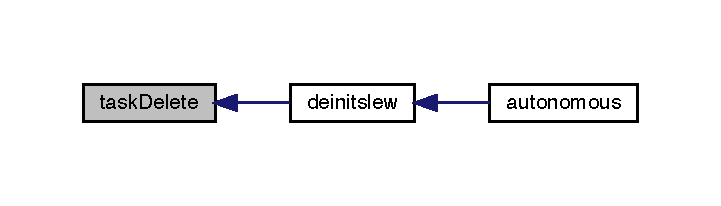
\includegraphics[width=346pt]{_a_p_i_8h_add3b8d580ea6ef5635c6d9ff88c68612_icgraph}
\end{center}
\end{figure}
\mbox{\label{_a_p_i_8h_a436fb5636d9a200ecebbb95968de91f6}} 
\index{A\+P\+I.\+h@{A\+P\+I.\+h}!task\+Get\+Count@{task\+Get\+Count}}
\index{task\+Get\+Count@{task\+Get\+Count}!A\+P\+I.\+h@{A\+P\+I.\+h}}
\paragraph{task\+Get\+Count()}
{\footnotesize\ttfamily unsigned int task\+Get\+Count (\begin{DoxyParamCaption}{ }\end{DoxyParamCaption})}

Determines the number of tasks that are currently being managed.

This includes all ready, blocked and suspended tasks. A task that has been deleted but not yet freed by the idle task will also be included in the count. Tasks recently created may take one context switch to be counted.

\begin{DoxyReturn}{Returns}
the number of tasks that are currently running, waiting, or suspended 
\end{DoxyReturn}
\mbox{\label{_a_p_i_8h_a4f805fd479cb4c427e8f4edfa7d55143}} 
\index{A\+P\+I.\+h@{A\+P\+I.\+h}!task\+Get\+State@{task\+Get\+State}}
\index{task\+Get\+State@{task\+Get\+State}!A\+P\+I.\+h@{A\+P\+I.\+h}}
\paragraph{task\+Get\+State()}
{\footnotesize\ttfamily unsigned int task\+Get\+State (\begin{DoxyParamCaption}\item[{\textbf{ Task\+Handle}}]{task }\end{DoxyParamCaption})}

Retrieves the state of the specified task. Note that the state of tasks which have died may be re-\/used for future tasks, causing the value returned by this function to reflect a different task than possibly intended in this case.


\begin{DoxyParams}{Parameters}
{\em task} & Handle to the task to query. Passing N\+U\+LL will query the current task status (which will, by definition, be T\+A\+S\+K\+\_\+\+R\+U\+N\+N\+I\+NG if this call returns)\\
\hline
\end{DoxyParams}
\begin{DoxyReturn}{Returns}
A value reflecting the task\textquotesingle{}s status, one of the constants T\+A\+S\+K\+\_\+\+D\+E\+AD, T\+A\+S\+K\+\_\+\+R\+U\+N\+N\+I\+NG, T\+A\+S\+K\+\_\+\+R\+U\+N\+N\+A\+B\+LE, T\+A\+S\+K\+\_\+\+S\+L\+E\+E\+P\+I\+NG, or T\+A\+S\+K\+\_\+\+S\+U\+S\+P\+E\+N\+D\+ED 
\end{DoxyReturn}
\mbox{\label{_a_p_i_8h_ae62d015b8280e4c74ad9ee15c7ac790b}} 
\index{A\+P\+I.\+h@{A\+P\+I.\+h}!task\+Priority\+Get@{task\+Priority\+Get}}
\index{task\+Priority\+Get@{task\+Priority\+Get}!A\+P\+I.\+h@{A\+P\+I.\+h}}
\paragraph{task\+Priority\+Get()}
{\footnotesize\ttfamily unsigned int task\+Priority\+Get (\begin{DoxyParamCaption}\item[{const \textbf{ Task\+Handle}}]{task }\end{DoxyParamCaption})}

Obtains the priority of the specified task.


\begin{DoxyParams}{Parameters}
{\em task} & the task to check; passing N\+U\+LL checks the current task \\
\hline
\end{DoxyParams}
\begin{DoxyReturn}{Returns}
the priority of that task from 0 to T\+A\+S\+K\+\_\+\+M\+A\+X\+\_\+\+P\+R\+I\+O\+R\+I\+T\+I\+ES 
\end{DoxyReturn}
\mbox{\label{_a_p_i_8h_a91d8f7074c6cb12dfe163df17bdf5540}} 
\index{A\+P\+I.\+h@{A\+P\+I.\+h}!task\+Priority\+Set@{task\+Priority\+Set}}
\index{task\+Priority\+Set@{task\+Priority\+Set}!A\+P\+I.\+h@{A\+P\+I.\+h}}
\paragraph{task\+Priority\+Set()}
{\footnotesize\ttfamily void task\+Priority\+Set (\begin{DoxyParamCaption}\item[{\textbf{ Task\+Handle}}]{task,  }\item[{const unsigned int}]{new\+Priority }\end{DoxyParamCaption})}

Sets the priority of the specified task.

A context switch may occur before the function returns if the priority being set is higher than the currently executing task and the task being mutated is available to be scheduled.


\begin{DoxyParams}{Parameters}
{\em task} & the task to change; passing N\+U\+LL changes the current task \\
\hline
{\em new\+Priority} & a value between T\+A\+S\+K\+\_\+\+P\+R\+I\+O\+R\+I\+T\+Y\+\_\+\+L\+O\+W\+E\+ST and T\+A\+S\+K\+\_\+\+P\+R\+I\+O\+R\+I\+T\+Y\+\_\+\+H\+I\+G\+H\+E\+ST inclusive indicating the new task priority \\
\hline
\end{DoxyParams}
\mbox{\label{_a_p_i_8h_afa2a4c5236b32bd9983bf19a4ac0cc23}} 
\index{A\+P\+I.\+h@{A\+P\+I.\+h}!task\+Resume@{task\+Resume}}
\index{task\+Resume@{task\+Resume}!A\+P\+I.\+h@{A\+P\+I.\+h}}
\paragraph{task\+Resume()}
{\footnotesize\ttfamily void task\+Resume (\begin{DoxyParamCaption}\item[{\textbf{ Task\+Handle}}]{task\+To\+Resume }\end{DoxyParamCaption})}

Resumes the specified task.

A task that has been suspended by one or more calls to \doxyref{task\+Suspend()}{p.}{_a_p_i_8h_ab56a51f337ad1903ad2bbce095744170} will be made available for scheduling again by a call to \doxyref{task\+Resume()}{p.}{_a_p_i_8h_afa2a4c5236b32bd9983bf19a4ac0cc23}. If the task was not suspended at the time of the call to \doxyref{task\+Resume()}{p.}{_a_p_i_8h_afa2a4c5236b32bd9983bf19a4ac0cc23}, undefined behavior occurs.


\begin{DoxyParams}{Parameters}
{\em task\+To\+Resume} & the task to change; passing N\+U\+LL is not allowed as the current task cannot be suspended (it is obviously running if this function is called) \\
\hline
\end{DoxyParams}
\mbox{\label{_a_p_i_8h_ab05a241d6d1fd98b1ceb4665db678156}} 
\index{A\+P\+I.\+h@{A\+P\+I.\+h}!task\+Run\+Loop@{task\+Run\+Loop}}
\index{task\+Run\+Loop@{task\+Run\+Loop}!A\+P\+I.\+h@{A\+P\+I.\+h}}
\paragraph{task\+Run\+Loop()}
{\footnotesize\ttfamily \textbf{ Task\+Handle} task\+Run\+Loop (\begin{DoxyParamCaption}\item[{void($\ast$)(void)}]{fn,  }\item[{const unsigned long}]{increment }\end{DoxyParamCaption})}

Starts a task which will periodically call the specified function.

Intended for use as a quick-\/start skeleton for cyclic tasks with higher priority than the \char`\"{}main\char`\"{} tasks. The created task will have priority T\+A\+S\+K\+\_\+\+P\+R\+I\+O\+R\+I\+T\+Y\+\_\+\+D\+E\+F\+A\+U\+LT + 1 with the default stack size. To customize behavior, create a task manually with the specified function.

This task will automatically terminate after one further function invocation when the robot is disabled or when the robot mode is switched.


\begin{DoxyParams}{Parameters}
{\em fn} & the function to call in this loop \\
\hline
{\em increment} & the delay between successive calls in milliseconds; the \doxyref{task\+Delay\+Until()}{p.}{_a_p_i_8h_ae93bc867b1aa4a12d6536a497f1b6869} function is used for accurate cycle timing \\
\hline
\end{DoxyParams}
\begin{DoxyReturn}{Returns}
a handle to the task, or N\+U\+LL if an error occurred 
\end{DoxyReturn}


Referenced by \textbf{ init\+\_\+localization()}, and \textbf{ init\+\_\+slew()}.

Here is the caller graph for this function\+:\nopagebreak
\begin{figure}[H]
\begin{center}
\leavevmode
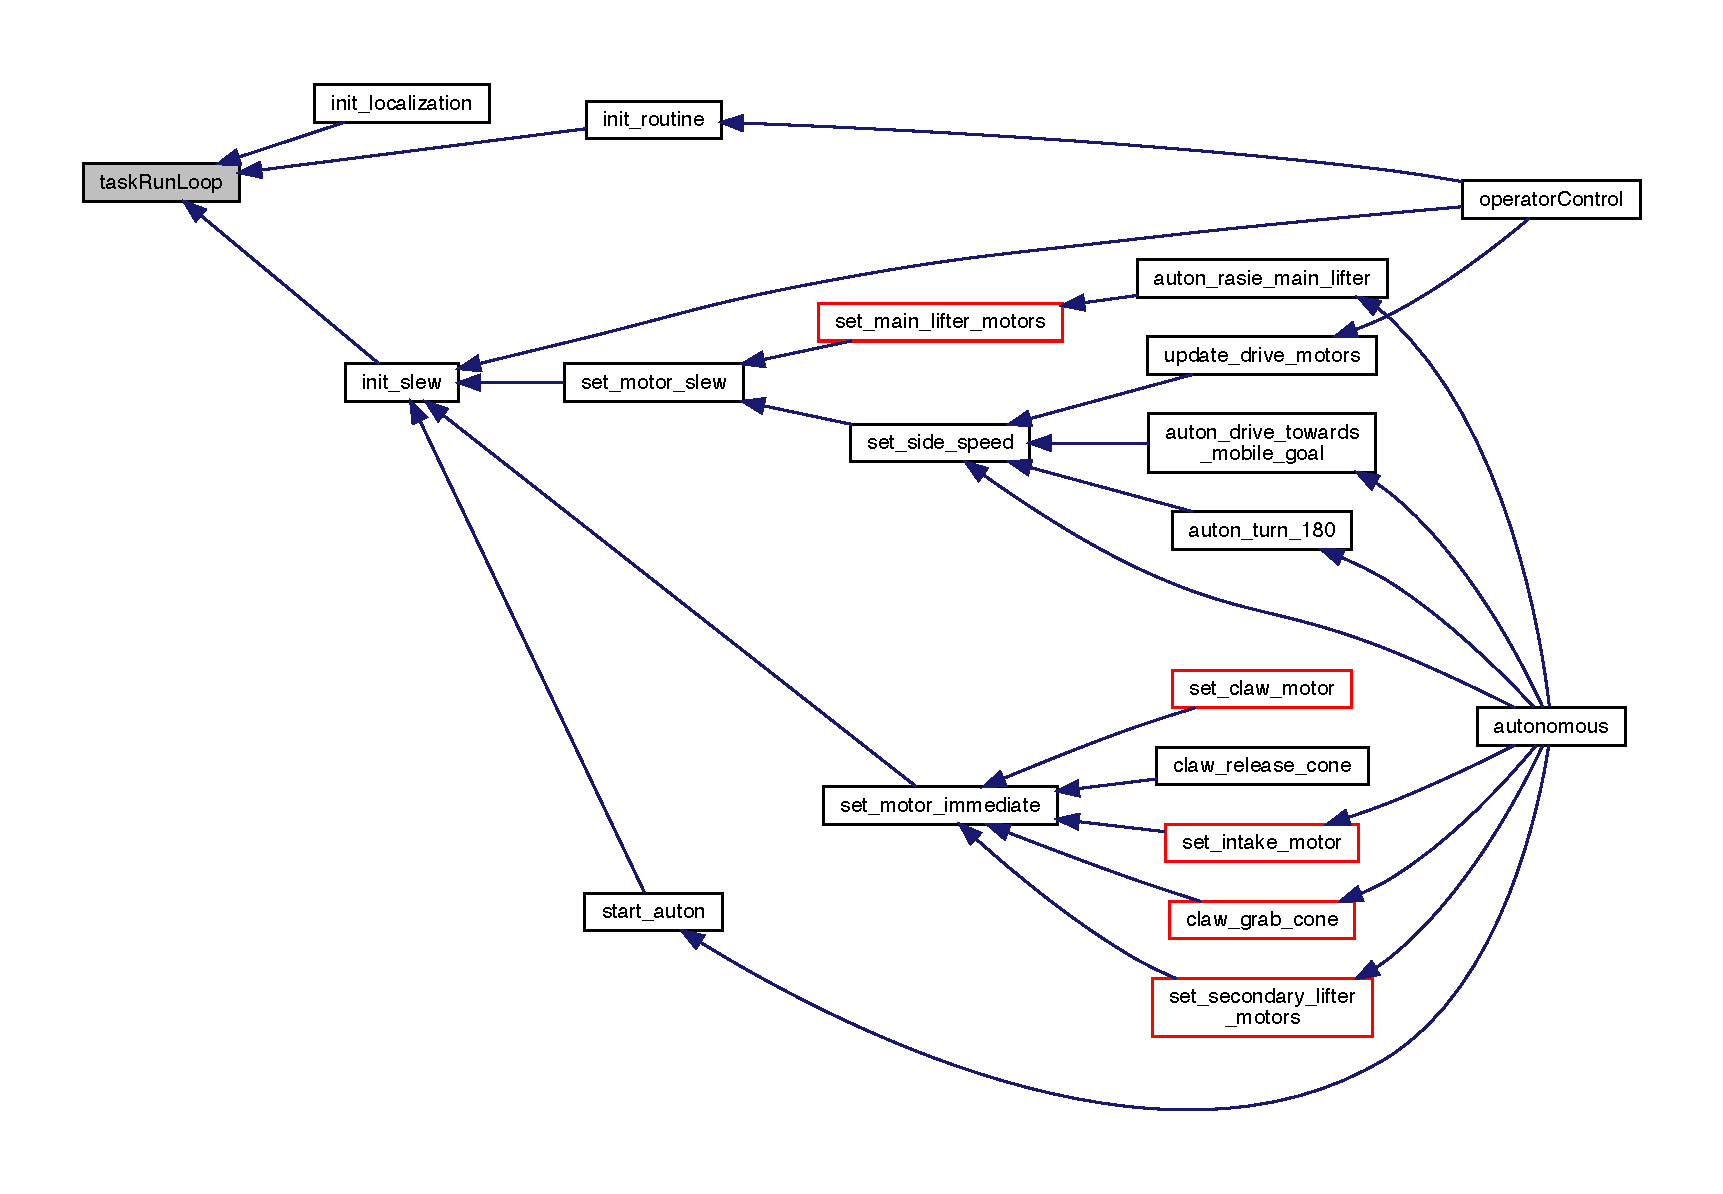
\includegraphics[width=350pt]{_a_p_i_8h_ab05a241d6d1fd98b1ceb4665db678156_icgraph}
\end{center}
\end{figure}
\mbox{\label{_a_p_i_8h_ab56a51f337ad1903ad2bbce095744170}} 
\index{A\+P\+I.\+h@{A\+P\+I.\+h}!task\+Suspend@{task\+Suspend}}
\index{task\+Suspend@{task\+Suspend}!A\+P\+I.\+h@{A\+P\+I.\+h}}
\paragraph{task\+Suspend()}
{\footnotesize\ttfamily void task\+Suspend (\begin{DoxyParamCaption}\item[{\textbf{ Task\+Handle}}]{task\+To\+Suspend }\end{DoxyParamCaption})}

Suspends the specified task.

When suspended a task will not be scheduled, regardless of whether it might be otherwise available to run.


\begin{DoxyParams}{Parameters}
{\em task\+To\+Suspend} & the task to suspend; passing N\+U\+LL suspends the current task \\
\hline
\end{DoxyParams}
\mbox{\label{_a_p_i_8h_a435d7fc1c3c3da80ed64cf9dfed0bd42}} 
\index{A\+P\+I.\+h@{A\+P\+I.\+h}!ultrasonic\+Get@{ultrasonic\+Get}}
\index{ultrasonic\+Get@{ultrasonic\+Get}!A\+P\+I.\+h@{A\+P\+I.\+h}}
\paragraph{ultrasonic\+Get()}
{\footnotesize\ttfamily int ultrasonic\+Get (\begin{DoxyParamCaption}\item[{\textbf{ Ultrasonic}}]{ult }\end{DoxyParamCaption})}

Gets the current ultrasonic sensor value in centimeters.

If no object was found or if the ultrasonic sensor is polled while it is pinging and waiting for a response, -\/1 (U\+L\+T\+R\+A\+\_\+\+B\+A\+D\+\_\+\+R\+E\+S\+P\+O\+N\+SE) is returned. If the ultrasonic sensor was never started, the return value is undefined. Round and fluffy objects can cause inaccurate values to be returned.


\begin{DoxyParams}{Parameters}
{\em ult} & the Ultrasonic object from \doxyref{ultrasonic\+Init()}{p.}{_a_p_i_8h_aed267558847e901e3741bd031c4fc83d} to read \\
\hline
\end{DoxyParams}
\begin{DoxyReturn}{Returns}
the distance to the nearest object in centimeters 
\end{DoxyReturn}
\mbox{\label{_a_p_i_8h_aed267558847e901e3741bd031c4fc83d}} 
\index{A\+P\+I.\+h@{A\+P\+I.\+h}!ultrasonic\+Init@{ultrasonic\+Init}}
\index{ultrasonic\+Init@{ultrasonic\+Init}!A\+P\+I.\+h@{A\+P\+I.\+h}}
\paragraph{ultrasonic\+Init()}
{\footnotesize\ttfamily \textbf{ Ultrasonic} ultrasonic\+Init (\begin{DoxyParamCaption}\item[{unsigned char}]{port\+Echo,  }\item[{unsigned char}]{port\+Ping }\end{DoxyParamCaption})}

Initializes an ultrasonic sensor on the specified digital ports.

The ultrasonic sensor will be polled in the background in concert with the other sensors registered using this method. N\+U\+LL will be returned if either port is invalid or the ultrasonic sensor port is already in use.


\begin{DoxyParams}{Parameters}
{\em port\+Echo} & the port connected to the orange cable from 1-\/9,11-\/12 \\
\hline
{\em port\+Ping} & the port connected to the yellow cable from 1-\/12 \\
\hline
\end{DoxyParams}
\begin{DoxyReturn}{Returns}
an Ultrasonic object to be stored and used for later calls to ultrasonic functions 
\end{DoxyReturn}
\mbox{\label{_a_p_i_8h_a355f91a286a081b95104b09898b467ed}} 
\index{A\+P\+I.\+h@{A\+P\+I.\+h}!ultrasonic\+Shutdown@{ultrasonic\+Shutdown}}
\index{ultrasonic\+Shutdown@{ultrasonic\+Shutdown}!A\+P\+I.\+h@{A\+P\+I.\+h}}
\paragraph{ultrasonic\+Shutdown()}
{\footnotesize\ttfamily void ultrasonic\+Shutdown (\begin{DoxyParamCaption}\item[{\textbf{ Ultrasonic}}]{ult }\end{DoxyParamCaption})}

Stops and disables the ultrasonic sensor.

The last distance it had before stopping will be retained. One more ping operation may occur before the sensor is fully disabled.


\begin{DoxyParams}{Parameters}
{\em ult} & the Ultrasonic object from \doxyref{ultrasonic\+Init()}{p.}{_a_p_i_8h_aed267558847e901e3741bd031c4fc83d} to stop \\
\hline
\end{DoxyParams}
\mbox{\label{_a_p_i_8h_a86066f3cf35f5fca7ec405189773182c}} 
\index{A\+P\+I.\+h@{A\+P\+I.\+h}!usart\+Init@{usart\+Init}}
\index{usart\+Init@{usart\+Init}!A\+P\+I.\+h@{A\+P\+I.\+h}}
\paragraph{usart\+Init()}
{\footnotesize\ttfamily void usart\+Init (\begin{DoxyParamCaption}\item[{\textbf{ P\+R\+O\+S\+\_\+\+F\+I\+LE} $\ast$}]{usart,  }\item[{unsigned int}]{baud,  }\item[{unsigned int}]{flags }\end{DoxyParamCaption})}

Initialize the specified serial interface with the given connection parameters.

I/O to the port is accomplished using the \char`\"{}standard\char`\"{} I/O functions such as \doxyref{fputs()}{p.}{_a_p_i_8h_ae4859a13f64d3dc4d57875512f0d1171}, \doxyref{fprintf()}{p.}{_a_p_i_8h_ab9989f4619e4d3ccb13ed4c36d5f787a}, and \doxyref{fputc()}{p.}{_a_p_i_8h_afe7d25ce198da1f8fec5a2dca770cb6a}.

Re-\/initializing an open port may cause loss of data in the buffers. This routine may be safely called from \doxyref{initialize\+I\+O()}{p.}{main_8h_ad9cda921edb01125bb13c2f86bcf624b} or when the scheduler is paused. If I/O is attempted on a serial port which has never been opened, the behavior will be the same as if the port had been disabled.


\begin{DoxyParams}{Parameters}
{\em usart} & the port to open, either \char`\"{}uart1\char`\"{} or \char`\"{}uart2\char`\"{} \\
\hline
{\em baud} & the baud rate to use from 2400 to 1000000 baud \\
\hline
{\em flags} & a bit mask combination of the S\+E\+R\+I\+A\+L\+\_\+$\ast$ flags specifying parity, stop, and data bits \\
\hline
\end{DoxyParams}
\mbox{\label{_a_p_i_8h_a802efaab0ca93c799eb82d42cf009e07}} 
\index{A\+P\+I.\+h@{A\+P\+I.\+h}!usart\+Shutdown@{usart\+Shutdown}}
\index{usart\+Shutdown@{usart\+Shutdown}!A\+P\+I.\+h@{A\+P\+I.\+h}}
\paragraph{usart\+Shutdown()}
{\footnotesize\ttfamily void usart\+Shutdown (\begin{DoxyParamCaption}\item[{\textbf{ P\+R\+O\+S\+\_\+\+F\+I\+LE} $\ast$}]{usart }\end{DoxyParamCaption})}

Disables the specified U\+S\+A\+RT interface.

Any data in the transmit and receive buffers will be lost. Attempts to read from the port when it is disabled will deadlock, and attempts to write to it may deadlock depending on the state of the buffer.


\begin{DoxyParams}{Parameters}
{\em usart} & the port to close, either \char`\"{}uart1\char`\"{} or \char`\"{}uart2\char`\"{} \\
\hline
\end{DoxyParams}
\mbox{\label{_a_p_i_8h_add8964052eef78ca864990642888a7d7}} 
\index{A\+P\+I.\+h@{A\+P\+I.\+h}!wait@{wait}}
\index{wait@{wait}!A\+P\+I.\+h@{A\+P\+I.\+h}}
\paragraph{wait()}
{\footnotesize\ttfamily void wait (\begin{DoxyParamCaption}\item[{const unsigned long}]{time }\end{DoxyParamCaption})}

Alias of \doxyref{task\+Delay()}{p.}{_a_p_i_8h_ac89618d0782547d189fe412a9917639b} intended to help EasyC users.


\begin{DoxyParams}{Parameters}
{\em time} & the duration of the delay in milliseconds (1 000 milliseconds per second) \\
\hline
\end{DoxyParams}
\mbox{\label{_a_p_i_8h_a591705c8bd27fce32490b0bd4fb7ecd9}} 
\index{A\+P\+I.\+h@{A\+P\+I.\+h}!wait\+Until@{wait\+Until}}
\index{wait\+Until@{wait\+Until}!A\+P\+I.\+h@{A\+P\+I.\+h}}
\paragraph{wait\+Until()}
{\footnotesize\ttfamily void wait\+Until (\begin{DoxyParamCaption}\item[{unsigned long $\ast$}]{previous\+Wake\+Time,  }\item[{const unsigned long}]{time }\end{DoxyParamCaption})}

Alias of \doxyref{task\+Delay\+Until()}{p.}{_a_p_i_8h_ae93bc867b1aa4a12d6536a497f1b6869} intended to help EasyC users.


\begin{DoxyParams}{Parameters}
{\em previous\+Wake\+Time} & a pointer to the last wakeup time \\
\hline
{\em time} & the duration of the delay in milliseconds (1 000 milliseconds per second) \\
\hline
\end{DoxyParams}
\mbox{\label{_a_p_i_8h_a8c2e4902f39a7abdea20cdf04007bb8e}} 
\index{A\+P\+I.\+h@{A\+P\+I.\+h}!watchdog\+Init@{watchdog\+Init}}
\index{watchdog\+Init@{watchdog\+Init}!A\+P\+I.\+h@{A\+P\+I.\+h}}
\paragraph{watchdog\+Init()}
{\footnotesize\ttfamily void watchdog\+Init (\begin{DoxyParamCaption}{ }\end{DoxyParamCaption})}

Enables I\+W\+DG watchdog timer which will reset the cortex if it locks up due to static shock or a misbehaving task preventing the timer to be reset. Not recovering from static shock will cause the robot to continue moving its motors indefinitely until turned off manually.

This function should only be called once in \doxyref{initialize\+I\+O()}{p.}{main_8h_ad9cda921edb01125bb13c2f86bcf624b} 

Referenced by \textbf{ initialize\+I\+O()}.

Here is the caller graph for this function\+:\nopagebreak
\begin{figure}[H]
\begin{center}
\leavevmode
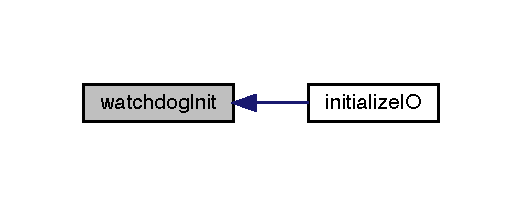
\includegraphics[width=250pt]{_a_p_i_8h_a8c2e4902f39a7abdea20cdf04007bb8e_icgraph}
\end{center}
\end{figure}


\subsubsection{Variable Documentation}
\mbox{\label{_a_p_i_8h_aa3800794cdb71dc374a5ce3e645e4bb4}} 
\index{A\+P\+I.\+h@{A\+P\+I.\+h}!format\+String@{format\+String}}
\index{format\+String@{format\+String}!A\+P\+I.\+h@{A\+P\+I.\+h}}
\paragraph{format\+String}
{\footnotesize\ttfamily void unsigned char const char$\ast$ format\+String}



Definition at line \textbf{ 1182} of file \textbf{ A\+P\+I.\+h}.

\mbox{\label{_a_p_i_8h_a58c3304a90ff2bb7064ff7187b2da466}} 
\index{A\+P\+I.\+h@{A\+P\+I.\+h}!line@{line}}
\index{line@{line}!A\+P\+I.\+h@{A\+P\+I.\+h}}
\paragraph{line}
{\footnotesize\ttfamily void unsigned char line}



Definition at line \textbf{ 1182} of file \textbf{ A\+P\+I.\+h}.


\section{include/controller.h File Reference}
\label{controller_8h}\index{include/controller.\+h@{include/controller.\+h}}


controller definitions, macros and functions to assist with usig the vex controllers.  


{\ttfamily \#include \char`\"{}vmath.\+h\char`\"{}}\newline
{\ttfamily \#include $<$A\+P\+I.\+h$>$}\newline
Include dependency graph for controller.\+h\+:\nopagebreak
\begin{figure}[H]
\begin{center}
\leavevmode
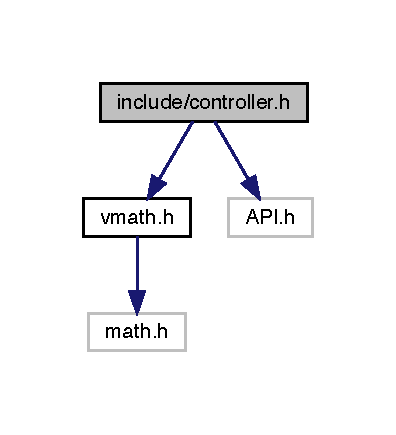
\includegraphics[width=190pt]{controller_8h__incl}
\end{center}
\end{figure}
This graph shows which files directly or indirectly include this file\+:\nopagebreak
\begin{figure}[H]
\begin{center}
\leavevmode
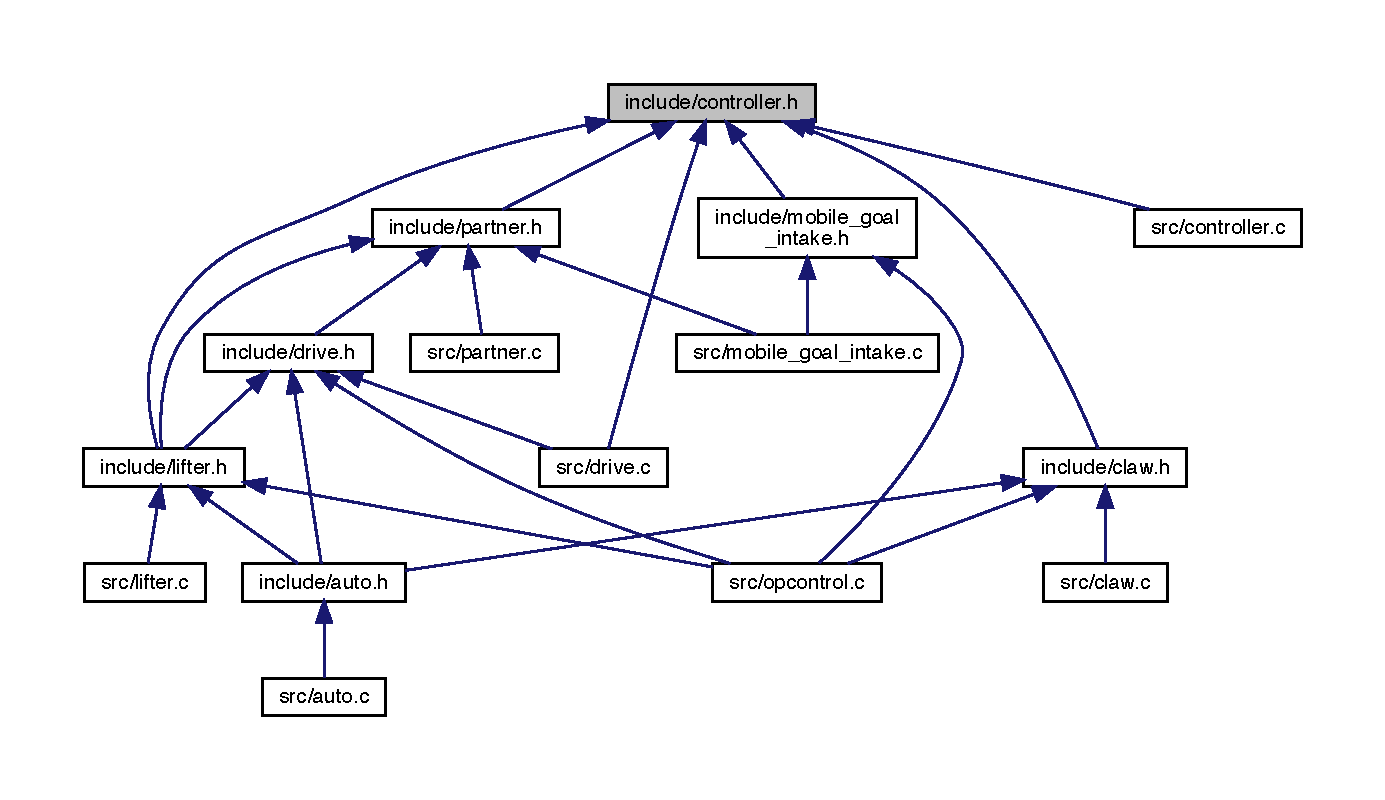
\includegraphics[width=350pt]{controller_8h__dep__incl}
\end{center}
\end{figure}
\subsection*{Macros}
\begin{DoxyCompactItemize}
\item 
\#define \textbf{ L\+E\+F\+T\+\_\+\+B\+U\+M\+P\+E\+RS}~6
\item 
\#define \textbf{ L\+E\+F\+T\+\_\+\+B\+U\+T\+T\+O\+NS}~7
\item 
\#define \textbf{ L\+E\+F\+T\+\_\+\+J\+O\+Y\+\_\+X}~4
\begin{DoxyCompactList}\small\item\em the left x joystick on controller \end{DoxyCompactList}\item 
\#define \textbf{ L\+E\+F\+T\+\_\+\+J\+O\+Y\+\_\+Y}~3
\begin{DoxyCompactList}\small\item\em the left y joystick on controller \end{DoxyCompactList}\item 
\#define \textbf{ M\+A\+S\+T\+ER}~1
\begin{DoxyCompactList}\small\item\em the master controller \end{DoxyCompactList}\item 
\#define \textbf{ P\+A\+R\+T\+N\+ER}~2
\begin{DoxyCompactList}\small\item\em the slave/partner controller \end{DoxyCompactList}\item 
\#define \textbf{ R\+I\+G\+H\+T\+\_\+\+B\+U\+M\+P\+E\+RS}~5
\item 
\#define \textbf{ R\+I\+G\+H\+T\+\_\+\+B\+U\+T\+T\+O\+NS}~8
\item 
\#define \textbf{ R\+I\+G\+H\+T\+\_\+\+J\+O\+Y\+\_\+X}~1
\begin{DoxyCompactList}\small\item\em the right x joystick on controller \end{DoxyCompactList}\item 
\#define \textbf{ R\+I\+G\+H\+T\+\_\+\+J\+O\+Y\+\_\+Y}~2
\begin{DoxyCompactList}\small\item\em the right y joystick on controller \end{DoxyCompactList}\end{DoxyCompactItemize}
\subsection*{Enumerations}
\begin{DoxyCompactItemize}
\item 
enum \textbf{ joystick} \{ \textbf{ R\+I\+G\+H\+T\+\_\+\+J\+OY}, 
\textbf{ L\+E\+F\+T\+\_\+\+J\+OY}
 \}\begin{DoxyCompactList}\small\item\em Represents a joystick on the controller. \end{DoxyCompactList}
\end{DoxyCompactItemize}
\subsection*{Functions}
\begin{DoxyCompactItemize}
\item 
struct \textbf{ cord} \textbf{ get\+\_\+joystick\+\_\+cord} (enum \textbf{ joystick} \textbf{ side}, int controller)
\begin{DoxyCompactList}\small\item\em Gets the location of a joystick on the controller. \end{DoxyCompactList}\end{DoxyCompactItemize}


\subsection{Detailed Description}
controller definitions, macros and functions to assist with usig the vex controllers. 

\begin{DoxyAuthor}{Author}
Chris Jerrett, Christian Desimone 
\end{DoxyAuthor}
\begin{DoxyDate}{Date}
9/9/2017 
\end{DoxyDate}


Definition in file \textbf{ controller.\+h}.



\subsection{Macro Definition Documentation}
\mbox{\label{controller_8h_ad61eb6d28a76985afb8d39ef925541bb}} 
\index{controller.\+h@{controller.\+h}!L\+E\+F\+T\+\_\+\+B\+U\+M\+P\+E\+RS@{L\+E\+F\+T\+\_\+\+B\+U\+M\+P\+E\+RS}}
\index{L\+E\+F\+T\+\_\+\+B\+U\+M\+P\+E\+RS@{L\+E\+F\+T\+\_\+\+B\+U\+M\+P\+E\+RS}!controller.\+h@{controller.\+h}}
\subsubsection{L\+E\+F\+T\+\_\+\+B\+U\+M\+P\+E\+RS}
{\footnotesize\ttfamily \#define L\+E\+F\+T\+\_\+\+B\+U\+M\+P\+E\+RS~6}



Definition at line \textbf{ 18} of file \textbf{ controller.\+h}.

\mbox{\label{controller_8h_a9b885de9f143efd0c862ceb054256536}} 
\index{controller.\+h@{controller.\+h}!L\+E\+F\+T\+\_\+\+B\+U\+T\+T\+O\+NS@{L\+E\+F\+T\+\_\+\+B\+U\+T\+T\+O\+NS}}
\index{L\+E\+F\+T\+\_\+\+B\+U\+T\+T\+O\+NS@{L\+E\+F\+T\+\_\+\+B\+U\+T\+T\+O\+NS}!controller.\+h@{controller.\+h}}
\subsubsection{L\+E\+F\+T\+\_\+\+B\+U\+T\+T\+O\+NS}
{\footnotesize\ttfamily \#define L\+E\+F\+T\+\_\+\+B\+U\+T\+T\+O\+NS~7}



Definition at line \textbf{ 16} of file \textbf{ controller.\+h}.

\mbox{\label{controller_8h_ac055a23829dc64aa20b8e2e1bcfbf316}} 
\index{controller.\+h@{controller.\+h}!L\+E\+F\+T\+\_\+\+J\+O\+Y\+\_\+X@{L\+E\+F\+T\+\_\+\+J\+O\+Y\+\_\+X}}
\index{L\+E\+F\+T\+\_\+\+J\+O\+Y\+\_\+X@{L\+E\+F\+T\+\_\+\+J\+O\+Y\+\_\+X}!controller.\+h@{controller.\+h}}
\subsubsection{L\+E\+F\+T\+\_\+\+J\+O\+Y\+\_\+X}
{\footnotesize\ttfamily \#define L\+E\+F\+T\+\_\+\+J\+O\+Y\+\_\+X~4}



the left x joystick on controller 

\begin{DoxyDate}{Date}
9/1/2017 
\end{DoxyDate}
\begin{DoxyAuthor}{Author}
Chris Jerrett 
\end{DoxyAuthor}


Definition at line \textbf{ 53} of file \textbf{ controller.\+h}.



Referenced by \textbf{ get\+\_\+joystick\+\_\+cord()}.

\mbox{\label{controller_8h_ae0a2b64db5fc4f4bf4b169185be93db3}} 
\index{controller.\+h@{controller.\+h}!L\+E\+F\+T\+\_\+\+J\+O\+Y\+\_\+Y@{L\+E\+F\+T\+\_\+\+J\+O\+Y\+\_\+Y}}
\index{L\+E\+F\+T\+\_\+\+J\+O\+Y\+\_\+Y@{L\+E\+F\+T\+\_\+\+J\+O\+Y\+\_\+Y}!controller.\+h@{controller.\+h}}
\subsubsection{L\+E\+F\+T\+\_\+\+J\+O\+Y\+\_\+Y}
{\footnotesize\ttfamily \#define L\+E\+F\+T\+\_\+\+J\+O\+Y\+\_\+Y~3}



the left y joystick on controller 

\begin{DoxyDate}{Date}
9/1/2017 
\end{DoxyDate}
\begin{DoxyAuthor}{Author}
Chris Jerrett 
\end{DoxyAuthor}


Definition at line \textbf{ 60} of file \textbf{ controller.\+h}.



Referenced by \textbf{ get\+\_\+joystick\+\_\+cord()}.

\mbox{\label{controller_8h_a3fa2d3bf1901157f734a584d47b25d8b}} 
\index{controller.\+h@{controller.\+h}!M\+A\+S\+T\+ER@{M\+A\+S\+T\+ER}}
\index{M\+A\+S\+T\+ER@{M\+A\+S\+T\+ER}!controller.\+h@{controller.\+h}}
\subsubsection{M\+A\+S\+T\+ER}
{\footnotesize\ttfamily \#define M\+A\+S\+T\+ER~1}



the master controller 

\begin{DoxyDate}{Date}
9/1/2017 
\end{DoxyDate}
\begin{DoxyAuthor}{Author}
Chris Jerrett 
\end{DoxyAuthor}


Definition at line \textbf{ 25} of file \textbf{ controller.\+h}.



Referenced by \textbf{ update\+\_\+drive\+\_\+motors()}, and \textbf{ update\+Intake()}.

\mbox{\label{controller_8h_a136e64cf351535da81cacb6a546cade6}} 
\index{controller.\+h@{controller.\+h}!P\+A\+R\+T\+N\+ER@{P\+A\+R\+T\+N\+ER}}
\index{P\+A\+R\+T\+N\+ER@{P\+A\+R\+T\+N\+ER}!controller.\+h@{controller.\+h}}
\subsubsection{P\+A\+R\+T\+N\+ER}
{\footnotesize\ttfamily \#define P\+A\+R\+T\+N\+ER~2}



the slave/partner controller 

\begin{DoxyDate}{Date}
9/1/2017 
\end{DoxyDate}
\begin{DoxyAuthor}{Author}
Chris Jerrett 
\end{DoxyAuthor}


Definition at line \textbf{ 32} of file \textbf{ controller.\+h}.



Referenced by \textbf{ update\+\_\+control()}, \textbf{ update\+\_\+drive\+\_\+motors()}, and \textbf{ update\+Intake()}.

\mbox{\label{controller_8h_a635896b08789914290171051d1b82465}} 
\index{controller.\+h@{controller.\+h}!R\+I\+G\+H\+T\+\_\+\+B\+U\+M\+P\+E\+RS@{R\+I\+G\+H\+T\+\_\+\+B\+U\+M\+P\+E\+RS}}
\index{R\+I\+G\+H\+T\+\_\+\+B\+U\+M\+P\+E\+RS@{R\+I\+G\+H\+T\+\_\+\+B\+U\+M\+P\+E\+RS}!controller.\+h@{controller.\+h}}
\subsubsection{R\+I\+G\+H\+T\+\_\+\+B\+U\+M\+P\+E\+RS}
{\footnotesize\ttfamily \#define R\+I\+G\+H\+T\+\_\+\+B\+U\+M\+P\+E\+RS~5}



Definition at line \textbf{ 17} of file \textbf{ controller.\+h}.

\mbox{\label{controller_8h_a68881b6085c880930037b20764fe5aee}} 
\index{controller.\+h@{controller.\+h}!R\+I\+G\+H\+T\+\_\+\+B\+U\+T\+T\+O\+NS@{R\+I\+G\+H\+T\+\_\+\+B\+U\+T\+T\+O\+NS}}
\index{R\+I\+G\+H\+T\+\_\+\+B\+U\+T\+T\+O\+NS@{R\+I\+G\+H\+T\+\_\+\+B\+U\+T\+T\+O\+NS}!controller.\+h@{controller.\+h}}
\subsubsection{R\+I\+G\+H\+T\+\_\+\+B\+U\+T\+T\+O\+NS}
{\footnotesize\ttfamily \#define R\+I\+G\+H\+T\+\_\+\+B\+U\+T\+T\+O\+NS~8}



Definition at line \textbf{ 15} of file \textbf{ controller.\+h}.

\mbox{\label{controller_8h_ad74f84aad465437cc1e0f914dbd6fab5}} 
\index{controller.\+h@{controller.\+h}!R\+I\+G\+H\+T\+\_\+\+J\+O\+Y\+\_\+X@{R\+I\+G\+H\+T\+\_\+\+J\+O\+Y\+\_\+X}}
\index{R\+I\+G\+H\+T\+\_\+\+J\+O\+Y\+\_\+X@{R\+I\+G\+H\+T\+\_\+\+J\+O\+Y\+\_\+X}!controller.\+h@{controller.\+h}}
\subsubsection{R\+I\+G\+H\+T\+\_\+\+J\+O\+Y\+\_\+X}
{\footnotesize\ttfamily \#define R\+I\+G\+H\+T\+\_\+\+J\+O\+Y\+\_\+X~1}



the right x joystick on controller 

\begin{DoxyDate}{Date}
9/1/2017 
\end{DoxyDate}
\begin{DoxyAuthor}{Author}
Chris Jerrett 
\end{DoxyAuthor}


Definition at line \textbf{ 39} of file \textbf{ controller.\+h}.



Referenced by \textbf{ get\+\_\+joystick\+\_\+cord()}.

\mbox{\label{controller_8h_a99457bf9dee795334411ea77f0858b16}} 
\index{controller.\+h@{controller.\+h}!R\+I\+G\+H\+T\+\_\+\+J\+O\+Y\+\_\+Y@{R\+I\+G\+H\+T\+\_\+\+J\+O\+Y\+\_\+Y}}
\index{R\+I\+G\+H\+T\+\_\+\+J\+O\+Y\+\_\+Y@{R\+I\+G\+H\+T\+\_\+\+J\+O\+Y\+\_\+Y}!controller.\+h@{controller.\+h}}
\subsubsection{R\+I\+G\+H\+T\+\_\+\+J\+O\+Y\+\_\+Y}
{\footnotesize\ttfamily \#define R\+I\+G\+H\+T\+\_\+\+J\+O\+Y\+\_\+Y~2}



the right y joystick on controller 

\begin{DoxyDate}{Date}
9/1/2017 
\end{DoxyDate}
\begin{DoxyAuthor}{Author}
Chris Jerrett 
\end{DoxyAuthor}


Definition at line \textbf{ 46} of file \textbf{ controller.\+h}.



Referenced by \textbf{ get\+\_\+joystick\+\_\+cord()}.



\subsection{Enumeration Type Documentation}
\mbox{\label{controller_8h_ac365c9e892abe4a1b85ae8f56a4eae5a}} 
\index{controller.\+h@{controller.\+h}!joystick@{joystick}}
\index{joystick@{joystick}!controller.\+h@{controller.\+h}}
\subsubsection{joystick}
{\footnotesize\ttfamily enum \textbf{ joystick}}



Represents a joystick on the controller. 

\begin{DoxyDate}{Date}
9/10/2017 
\end{DoxyDate}
\begin{DoxyAuthor}{Author}
Chris Jerrett 
\end{DoxyAuthor}
\begin{DoxyEnumFields}{Enumerator}
\raisebox{\heightof{T}}[0pt][0pt]{\index{R\+I\+G\+H\+T\+\_\+\+J\+OY@{R\+I\+G\+H\+T\+\_\+\+J\+OY}!controller.\+h@{controller.\+h}}\index{controller.\+h@{controller.\+h}!R\+I\+G\+H\+T\+\_\+\+J\+OY@{R\+I\+G\+H\+T\+\_\+\+J\+OY}}}\mbox{\label{controller_8h_ac365c9e892abe4a1b85ae8f56a4eae5aae08a2d362c677f96f72d93047513cafe}} 
R\+I\+G\+H\+T\+\_\+\+J\+OY&The right joystick \\
\hline

\raisebox{\heightof{T}}[0pt][0pt]{\index{L\+E\+F\+T\+\_\+\+J\+OY@{L\+E\+F\+T\+\_\+\+J\+OY}!controller.\+h@{controller.\+h}}\index{controller.\+h@{controller.\+h}!L\+E\+F\+T\+\_\+\+J\+OY@{L\+E\+F\+T\+\_\+\+J\+OY}}}\mbox{\label{controller_8h_ac365c9e892abe4a1b85ae8f56a4eae5aaf822d7888862e67a3c624775b85c50a9}} 
L\+E\+F\+T\+\_\+\+J\+OY&The left joystick \\
\hline

\end{DoxyEnumFields}


Definition at line \textbf{ 67} of file \textbf{ controller.\+h}.


\begin{DoxyCode}
00067               \{
00069   RIGHT_JOY,
00071   LEFT_JOY,
00072 \};
\end{DoxyCode}


\subsection{Function Documentation}
\mbox{\label{controller_8h_a0ce0176099c0bb15ad8c36123222059d}} 
\index{controller.\+h@{controller.\+h}!get\+\_\+joystick\+\_\+cord@{get\+\_\+joystick\+\_\+cord}}
\index{get\+\_\+joystick\+\_\+cord@{get\+\_\+joystick\+\_\+cord}!controller.\+h@{controller.\+h}}
\subsubsection{get\+\_\+joystick\+\_\+cord()}
{\footnotesize\ttfamily struct \textbf{ cord} get\+\_\+joystick\+\_\+cord (\begin{DoxyParamCaption}\item[{enum \textbf{ joystick}}]{side,  }\item[{int}]{controller }\end{DoxyParamCaption})}



Gets the location of a joystick on the controller. 

\begin{DoxyAuthor}{Author}
Chris Jerrett 
\end{DoxyAuthor}


Definition at line \textbf{ 7} of file \textbf{ controller.\+c}.



References \textbf{ L\+E\+F\+T\+\_\+\+J\+O\+Y\+\_\+X}, \textbf{ L\+E\+F\+T\+\_\+\+J\+O\+Y\+\_\+Y}, \textbf{ R\+I\+G\+H\+T\+\_\+\+J\+OY}, \textbf{ R\+I\+G\+H\+T\+\_\+\+J\+O\+Y\+\_\+X}, \textbf{ R\+I\+G\+H\+T\+\_\+\+J\+O\+Y\+\_\+Y}, \textbf{ cord\+::x}, and \textbf{ cord\+::y}.


\begin{DoxyCode}
00007                                                                   \{
00008   \textcolor{keywordtype}{int} x;
00009   \textcolor{keywordtype}{int} y;
00010   \textcolor{comment}{//Get the joystick value for either the right or left,}
00011   \textcolor{comment}{//depending on the mode}
00012   \textcolor{keywordflow}{if}(side == RIGHT_JOY) \{
00013     y = joystickGetAnalog(controller, RIGHT_JOY_X);
00014     x = joystickGetAnalog(controller, RIGHT_JOY_Y);
00015   \} \textcolor{keywordflow}{else} \{
00016     y = joystickGetAnalog(controller, LEFT_JOY_X);
00017     x = joystickGetAnalog(controller, LEFT_JOY_Y);
00018   \}
00019   \textcolor{comment}{//Define a coordinate for the joystick value}
00020   \textcolor{keyword}{struct }cord c;
00021   c.x = x;
00022   c.y = y;
00023   \textcolor{keywordflow}{return} c;
00024 \}
\end{DoxyCode}

\subsection{include/drive.h File Reference}
\label{drive_8h}\index{include/drive.\+h@{include/drive.\+h}}


Drive base definitions and enumerations.  


{\ttfamily \#include $<$A\+P\+I.\+h$>$}\newline
{\ttfamily \#include \char`\"{}partner.\+h\char`\"{}}\newline
Include dependency graph for drive.\+h\+:\nopagebreak
\begin{figure}[H]
\begin{center}
\leavevmode
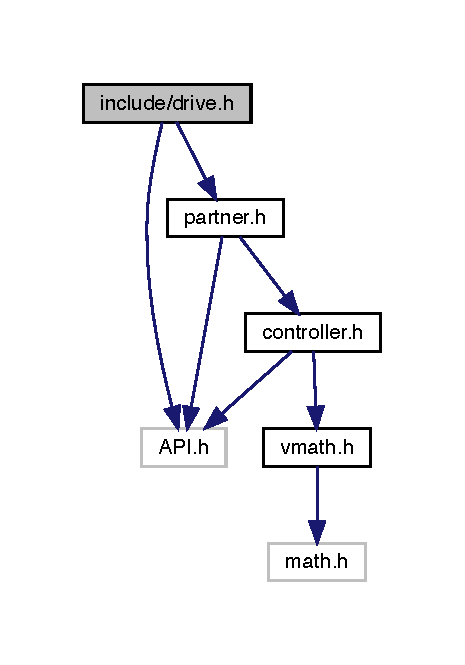
\includegraphics[width=350pt]{drive_8h__incl}
\end{center}
\end{figure}
This graph shows which files directly or indirectly include this file\+:\nopagebreak
\begin{figure}[H]
\begin{center}
\leavevmode
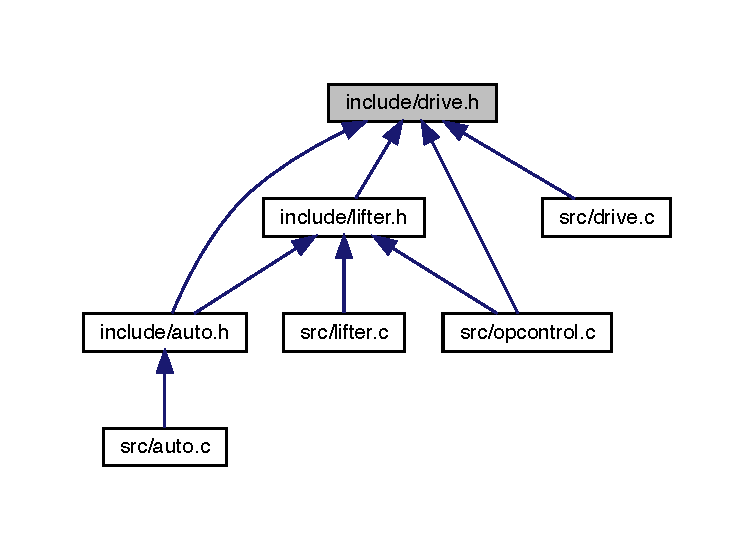
\includegraphics[width=350pt]{drive_8h__dep__incl}
\end{center}
\end{figure}
\subsubsection*{Macros}
\begin{DoxyCompactItemize}
\item 
\#define \textbf{ T\+H\+R\+E\+S\+H\+O\+LD}~10
\begin{DoxyCompactList}\small\item\em The dead spot on the controller to avoid running motors at low speeds. \end{DoxyCompactList}\end{DoxyCompactItemize}
\subsubsection*{Typedefs}
\begin{DoxyCompactItemize}
\item 
typedef enum \textbf{ side} \textbf{ side\+\_\+t}
\begin{DoxyCompactList}\small\item\em enumeration indication side of the robot. \end{DoxyCompactList}\end{DoxyCompactItemize}
\subsubsection*{Enumerations}
\begin{DoxyCompactItemize}
\item 
enum \textbf{ side} \{ \textbf{ L\+E\+FT}, 
\textbf{ B\+O\+TH}, 
\textbf{ R\+I\+G\+HT}
 \}\begin{DoxyCompactList}\small\item\em enumeration indication side of the robot. \end{DoxyCompactList}
\end{DoxyCompactItemize}
\subsubsection*{Functions}
\begin{DoxyCompactItemize}
\item 
void \textbf{ set\+\_\+side\+\_\+speed} (\textbf{ side\+\_\+t} \textbf{ side}, int speed)
\begin{DoxyCompactList}\small\item\em sets the speed of one side of the robot. \end{DoxyCompactList}\item 
void \textbf{ set\+Thresh} (int t)
\begin{DoxyCompactList}\small\item\em Sets the deadzone threshhold on the drive. \end{DoxyCompactList}\item 
void \textbf{ update\+\_\+drive\+\_\+motors} ()
\begin{DoxyCompactList}\small\item\em Updates the drive motors during teleop. \end{DoxyCompactList}\end{DoxyCompactItemize}


\subsubsection{Detailed Description}
Drive base definitions and enumerations. 

\begin{DoxyAuthor}{Author}
Chris Jerrett 
\end{DoxyAuthor}
\begin{DoxyDate}{Date}
9/9/2017 
\end{DoxyDate}


Definition in file \textbf{ drive.\+h}.



\subsubsection{Macro Definition Documentation}
\mbox{\label{drive_8h_a4679d8ea8690999a6c6c7c0cb245c879}} 
\index{drive.\+h@{drive.\+h}!T\+H\+R\+E\+S\+H\+O\+LD@{T\+H\+R\+E\+S\+H\+O\+LD}}
\index{T\+H\+R\+E\+S\+H\+O\+LD@{T\+H\+R\+E\+S\+H\+O\+LD}!drive.\+h@{drive.\+h}}
\paragraph{T\+H\+R\+E\+S\+H\+O\+LD}
{\footnotesize\ttfamily \#define T\+H\+R\+E\+S\+H\+O\+LD~10}



The dead spot on the controller to avoid running motors at low speeds. 



Definition at line \textbf{ 18} of file \textbf{ drive.\+h}.



Referenced by \textbf{ joystick\+Exp()}, and \textbf{ update\+\_\+lifter()}.



\subsubsection{Typedef Documentation}
\mbox{\label{drive_8h_a9df2afd2f1acb97019655e5e730609c7}} 
\index{drive.\+h@{drive.\+h}!side\+\_\+t@{side\+\_\+t}}
\index{side\+\_\+t@{side\+\_\+t}!drive.\+h@{drive.\+h}}
\paragraph{side\+\_\+t}
{\footnotesize\ttfamily typedef enum \textbf{ side}  \textbf{ side\+\_\+t}}



enumeration indication side of the robot. 

\begin{DoxyAuthor}{Author}
Christian Desimone 
\end{DoxyAuthor}
\begin{DoxyDate}{Date}
9/7/2017 Side can be right, both of left. Contained in side typedef, so enum is unnecessary. 
\end{DoxyDate}


\subsubsection{Enumeration Type Documentation}
\mbox{\label{drive_8h_afc015eff6557e84151d2e53b94375445}} 
\index{drive.\+h@{drive.\+h}!side@{side}}
\index{side@{side}!drive.\+h@{drive.\+h}}
\paragraph{side}
{\footnotesize\ttfamily enum \textbf{ side}}



enumeration indication side of the robot. 

\begin{DoxyAuthor}{Author}
Christian Desimone 
\end{DoxyAuthor}
\begin{DoxyDate}{Date}
9/7/2017 Side can be right, both of left. Contained in side typedef, so enum is unnecessary. 
\end{DoxyDate}
\begin{DoxyEnumFields}{Enumerator}
\raisebox{\heightof{T}}[0pt][0pt]{\index{L\+E\+FT@{L\+E\+FT}!drive.\+h@{drive.\+h}}\index{drive.\+h@{drive.\+h}!L\+E\+FT@{L\+E\+FT}}}\mbox{\label{drive_8h_afc015eff6557e84151d2e53b94375445adb45120aafd37a973140edee24708065}} 
L\+E\+FT&\\
\hline

\raisebox{\heightof{T}}[0pt][0pt]{\index{B\+O\+TH@{B\+O\+TH}!drive.\+h@{drive.\+h}}\index{drive.\+h@{drive.\+h}!B\+O\+TH@{B\+O\+TH}}}\mbox{\label{drive_8h_afc015eff6557e84151d2e53b94375445a627abe5a430420baf29ebe1940a7f2fb}} 
B\+O\+TH&\\
\hline

\raisebox{\heightof{T}}[0pt][0pt]{\index{R\+I\+G\+HT@{R\+I\+G\+HT}!drive.\+h@{drive.\+h}}\index{drive.\+h@{drive.\+h}!R\+I\+G\+HT@{R\+I\+G\+HT}}}\mbox{\label{drive_8h_afc015eff6557e84151d2e53b94375445aec8379af7490bb9eaaf579cf17876f38}} 
R\+I\+G\+HT&\\
\hline

\end{DoxyEnumFields}


Definition at line \textbf{ 26} of file \textbf{ drive.\+h}.


\begin{DoxyCode}
00026                  \{
00027   LEFT,
00028   BOTH,
00029   RIGHT
00030 \} side_t;
\end{DoxyCode}


\subsubsection{Function Documentation}
\mbox{\label{drive_8h_a8df41fd50094c065eedc81fc5e6595d1}} 
\index{drive.\+h@{drive.\+h}!set\+\_\+side\+\_\+speed@{set\+\_\+side\+\_\+speed}}
\index{set\+\_\+side\+\_\+speed@{set\+\_\+side\+\_\+speed}!drive.\+h@{drive.\+h}}
\paragraph{set\+\_\+side\+\_\+speed()}
{\footnotesize\ttfamily void set\+\_\+side\+\_\+speed (\begin{DoxyParamCaption}\item[{\textbf{ side\+\_\+t}}]{side,  }\item[{int}]{speed }\end{DoxyParamCaption})}



sets the speed of one side of the robot. 

\begin{DoxyAuthor}{Author}
Christian Desimone 
\end{DoxyAuthor}

\begin{DoxyParams}{Parameters}
{\em side} & a side enum which indicates the size. \\
\hline
{\em speed} & the speed of the side. Can range from -\/127 -\/ 127 negative being back and positive forwards \\
\hline
\end{DoxyParams}


Definition at line \textbf{ 68} of file \textbf{ drive.\+c}.



References \textbf{ B\+O\+TH}, \textbf{ L\+E\+FT}, \textbf{ M\+O\+T\+O\+R\+\_\+\+B\+A\+C\+K\+\_\+\+L\+E\+FT}, \textbf{ M\+O\+T\+O\+R\+\_\+\+B\+A\+C\+K\+\_\+\+R\+I\+G\+HT}, \textbf{ M\+O\+T\+O\+R\+\_\+\+F\+R\+O\+N\+T\+\_\+\+L\+E\+FT}, \textbf{ M\+O\+T\+O\+R\+\_\+\+F\+R\+O\+N\+T\+\_\+\+R\+I\+G\+HT}, \textbf{ M\+O\+T\+O\+R\+\_\+\+M\+I\+D\+D\+L\+E\+\_\+\+L\+E\+FT}, \textbf{ M\+O\+T\+O\+R\+\_\+\+M\+I\+D\+D\+L\+E\+\_\+\+R\+I\+G\+HT}, \textbf{ R\+I\+G\+HT}, and \textbf{ set\+\_\+motor\+\_\+slew()}.



Referenced by \textbf{ autonomous()}, and \textbf{ update\+\_\+drive\+\_\+motors()}.


\begin{DoxyCode}
00068                                            \{
00069   \textcolor{keywordflow}{if}(side == RIGHT || side == BOTH)\{
00070     set_motor_slew(MOTOR_BACK_RIGHT , -speed);
00071     set_motor_slew(MOTOR_FRONT_RIGHT, -speed);
00072     set_motor_slew(MOTOR_MIDDLE_RIGHT, -speed);
00073   \}
00074   \textcolor{keywordflow}{if}(side == LEFT || side == BOTH)\{
00075     set_motor_slew(MOTOR_BACK_LEFT, speed);
00076     set_motor_slew(MOTOR_MIDDLE_LEFT, speed);
00077     set_motor_slew(MOTOR_FRONT_LEFT, speed);
00078   \}
00079 \}
\end{DoxyCode}
Here is the call graph for this function\+:\nopagebreak
\begin{figure}[H]
\begin{center}
\leavevmode
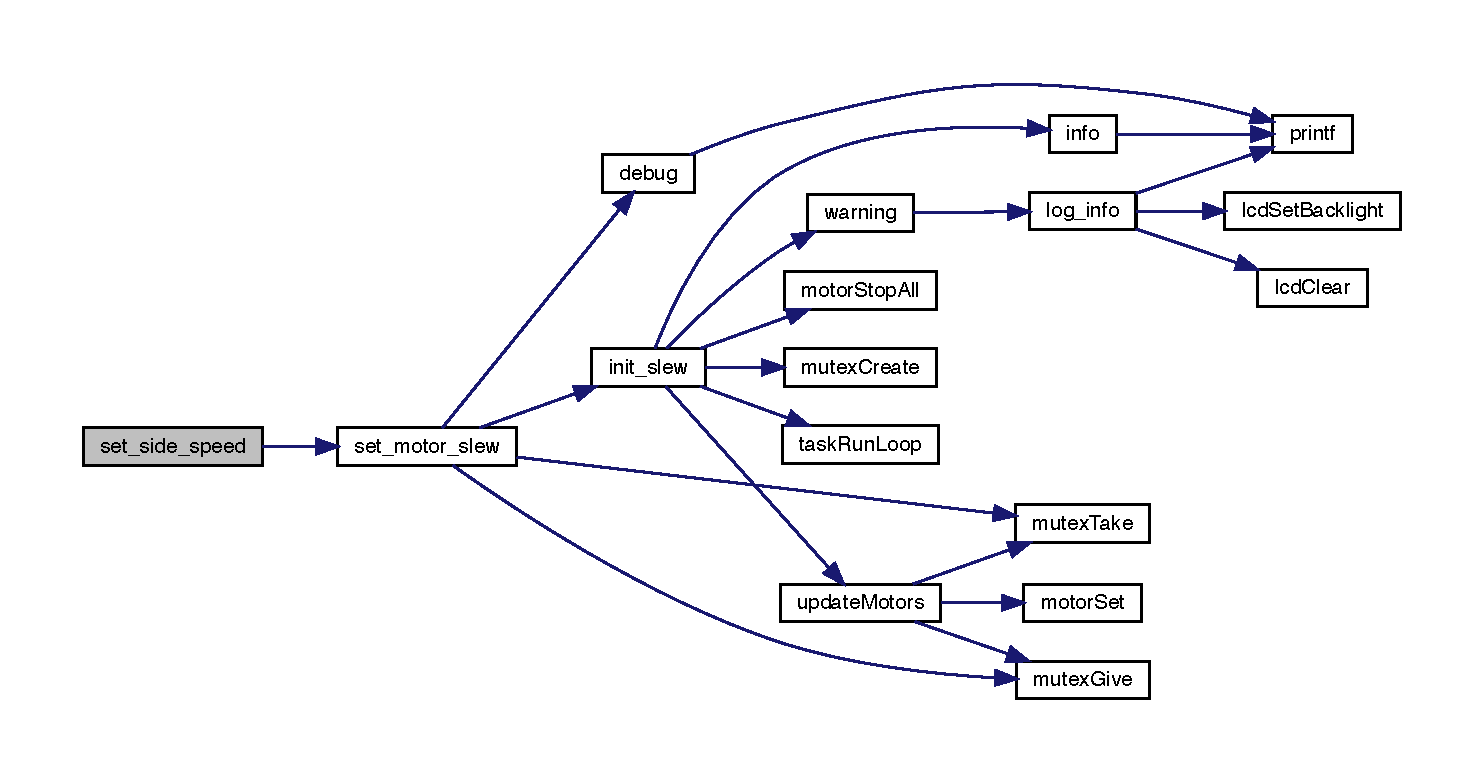
\includegraphics[width=350pt]{drive_8h_a8df41fd50094c065eedc81fc5e6595d1_cgraph}
\end{center}
\end{figure}
Here is the caller graph for this function\+:\nopagebreak
\begin{figure}[H]
\begin{center}
\leavevmode
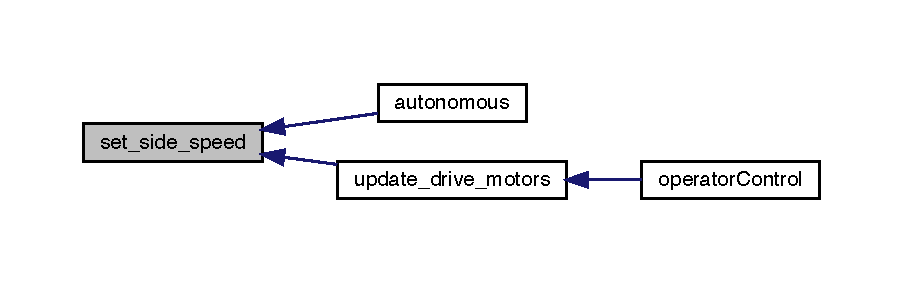
\includegraphics[width=350pt]{drive_8h_a8df41fd50094c065eedc81fc5e6595d1_icgraph}
\end{center}
\end{figure}
\mbox{\label{drive_8h_a53d6e35d53ec3e0b1b1c489d8203f204}} 
\index{drive.\+h@{drive.\+h}!set\+Thresh@{set\+Thresh}}
\index{set\+Thresh@{set\+Thresh}!drive.\+h@{drive.\+h}}
\paragraph{set\+Thresh()}
{\footnotesize\ttfamily void set\+Thresh (\begin{DoxyParamCaption}\item[{int}]{t }\end{DoxyParamCaption})}



Sets the deadzone threshhold on the drive. 

\begin{DoxyAuthor}{Author}
Chris Jerrett

Christian Desimone 
\end{DoxyAuthor}


Definition at line \textbf{ 25} of file \textbf{ drive.\+c}.



References \textbf{ thresh}.


\begin{DoxyCode}
00025                      \{
00026   thresh = t;
00027 \}
\end{DoxyCode}
\mbox{\label{drive_8h_a8224a4626a934d30ed587671b7004bf8}} 
\index{drive.\+h@{drive.\+h}!update\+\_\+drive\+\_\+motors@{update\+\_\+drive\+\_\+motors}}
\index{update\+\_\+drive\+\_\+motors@{update\+\_\+drive\+\_\+motors}!drive.\+h@{drive.\+h}}
\paragraph{update\+\_\+drive\+\_\+motors()}
{\footnotesize\ttfamily void update\+\_\+drive\+\_\+motors (\begin{DoxyParamCaption}{ }\end{DoxyParamCaption})}



Updates the drive motors during teleop. 

\begin{DoxyAuthor}{Author}
Christian Desimone 
\end{DoxyAuthor}
\begin{DoxyDate}{Date}
9/5/17 
\end{DoxyDate}


Definition at line \textbf{ 34} of file \textbf{ drive.\+c}.



References \textbf{ get\+\_\+mode()}, \textbf{ joystick\+Get\+Analog()}, \textbf{ L\+E\+FT}, \textbf{ M\+A\+S\+T\+ER}, \textbf{ P\+A\+R\+T\+N\+ER}, \textbf{ P\+A\+R\+T\+N\+E\+R\+\_\+\+C\+O\+N\+T\+R\+O\+L\+L\+E\+R\+\_\+\+M\+O\+DE}, \textbf{ R\+I\+G\+HT}, \textbf{ set\+\_\+side\+\_\+speed()}, \textbf{ thresh}, \textbf{ cord\+::x}, and \textbf{ cord\+::y}.



Referenced by \textbf{ operator\+Control()}.


\begin{DoxyCode}
00034                           \{
00035   \textcolor{comment}{//Get the joystick values from the controller}
00036   \textcolor{keywordtype}{int} x = 0;
00037   \textcolor{keywordtype}{int} y = 0;
00038   \textcolor{keywordflow}{if}(get_mode() == PARTNER_CONTROLLER_MODE) \{
00039     x = (joystickGetAnalog(PARTNER, 3));
00040     y = (joystickGetAnalog(PARTNER, 1));
00041   \} \textcolor{keywordflow}{else} \{
00042     x = -(joystickGetAnalog(MASTER, 3));
00043     y = (joystickGetAnalog(MASTER, 1));
00044   \}
00045   \textcolor{comment}{//Make sure the joystick values are significant enough to change the motors}
00046   \textcolor{keywordflow}{if}(x < thresh && x > -thresh)\{
00047     x = 0;
00048   \}
00049   \textcolor{keywordflow}{if}(y < thresh && y > -thresh)\{
00050     y = 0;
00051   \}
00052   \textcolor{comment}{//Create motor values for the left and right from the x and y of the joystick}
00053   \textcolor{keywordtype}{int} r = (x + y);
00054   \textcolor{keywordtype}{int} l = -(x - y);
00055 
00056   \textcolor{comment}{//Set the drive motors}
00057   set_side_speed(LEFT, l);
00058   set_side_speed(RIGHT, -r);
00059 
00060 \}
\end{DoxyCode}
Here is the call graph for this function\+:\nopagebreak
\begin{figure}[H]
\begin{center}
\leavevmode
\includegraphics[width=350pt]{drive_8h_a8224a4626a934d30ed587671b7004bf8_cgraph}
\end{center}
\end{figure}
Here is the caller graph for this function\+:\nopagebreak
\begin{figure}[H]
\begin{center}
\leavevmode
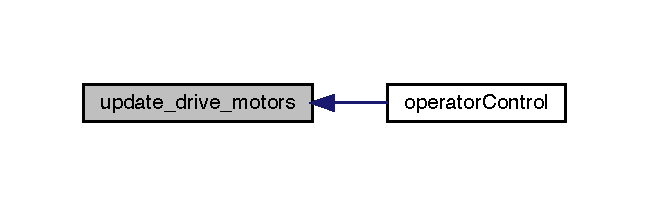
\includegraphics[width=311pt]{drive_8h_a8224a4626a934d30ed587671b7004bf8_icgraph}
\end{center}
\end{figure}

\hypertarget{encoders_8h}{}\section{include/encoders.h File Reference}
\label{encoders_8h}\index{include/encoders.\+h@{include/encoders.\+h}}


wrapper around encoder functions  


{\ttfamily \#include $<$A\+P\+I.\+h$>$}\newline
\subsection*{Macros}
\begin{DoxyCompactItemize}
\item 
\#define \hyperlink{encoders_8h_a87db35d2735ef045f57d446b3bfe8d48}{I\+M\+E\+\_\+\+N\+U\+M\+B\+ER}~0
\begin{DoxyCompactList}\small\item\em The number of I\+M\+Es. This number is compared against the number detect in init\+\_\+encoders. \end{DoxyCompactList}\end{DoxyCompactItemize}
\subsection*{Functions}
\begin{DoxyCompactItemize}
\item 
int \hyperlink{encoders_8h_aed261dd4dae33a48c42f2e363c84760f}{get\+\_\+encoder\+\_\+ticks} (unsigned char address)
\begin{DoxyCompactList}\small\item\em Gets the encoder ticks since last reset. \end{DoxyCompactList}\item 
int \hyperlink{encoders_8h_a8e6b77703c5cf18e00709b052fb4bf22}{get\+\_\+encoder\+\_\+velocity} (unsigned char address)
\begin{DoxyCompactList}\small\item\em Gets the encoder reads. \end{DoxyCompactList}\item 
bool \hyperlink{encoders_8h_aa6ec1ca17e907babd52803ecba451cd3}{init\+\_\+encoders} ()
\begin{DoxyCompactList}\small\item\em Initializes all motor encoders. \end{DoxyCompactList}\end{DoxyCompactItemize}


\subsection{Detailed Description}
wrapper around encoder functions 

\begin{DoxyAuthor}{Author}
Chris Jerrett 
\end{DoxyAuthor}
\begin{DoxyDate}{Date}
9/9/2017 
\end{DoxyDate}


\subsection{Macro Definition Documentation}
\mbox{\Hypertarget{encoders_8h_a87db35d2735ef045f57d446b3bfe8d48}\label{encoders_8h_a87db35d2735ef045f57d446b3bfe8d48}} 
\index{encoders.\+h@{encoders.\+h}!I\+M\+E\+\_\+\+N\+U\+M\+B\+ER@{I\+M\+E\+\_\+\+N\+U\+M\+B\+ER}}
\index{I\+M\+E\+\_\+\+N\+U\+M\+B\+ER@{I\+M\+E\+\_\+\+N\+U\+M\+B\+ER}!encoders.\+h@{encoders.\+h}}
\subsubsection{\texorpdfstring{I\+M\+E\+\_\+\+N\+U\+M\+B\+ER}{IME\_NUMBER}}
{\footnotesize\ttfamily \#define I\+M\+E\+\_\+\+N\+U\+M\+B\+ER~0}



The number of I\+M\+Es. This number is compared against the number detect in init\+\_\+encoders. 

\begin{DoxySeeAlso}{See also}
\hyperlink{encoders_8h_aa6ec1ca17e907babd52803ecba451cd3}{init\+\_\+encoders()} 
\end{DoxySeeAlso}
\begin{DoxyAuthor}{Author}
Chris Jerrett 
\end{DoxyAuthor}
\begin{DoxyDate}{Date}
9/9/2017 
\end{DoxyDate}
\begin{DoxySeeAlso}{See also}
\hyperlink{encoders_8h_a87db35d2735ef045f57d446b3bfe8d48}{I\+M\+E\+\_\+\+N\+U\+M\+B\+ER} 
\end{DoxySeeAlso}


Definition at line 21 of file encoders.\+h.



Referenced by init\+\_\+encoders().



\subsection{Function Documentation}
\mbox{\Hypertarget{encoders_8h_aed261dd4dae33a48c42f2e363c84760f}\label{encoders_8h_aed261dd4dae33a48c42f2e363c84760f}} 
\index{encoders.\+h@{encoders.\+h}!get\+\_\+encoder\+\_\+ticks@{get\+\_\+encoder\+\_\+ticks}}
\index{get\+\_\+encoder\+\_\+ticks@{get\+\_\+encoder\+\_\+ticks}!encoders.\+h@{encoders.\+h}}
\subsubsection{\texorpdfstring{get\+\_\+encoder\+\_\+ticks()}{get\_encoder\_ticks()}}
{\footnotesize\ttfamily int get\+\_\+encoder\+\_\+ticks (\begin{DoxyParamCaption}\item[{unsigned char}]{address }\end{DoxyParamCaption})}



Gets the encoder ticks since last reset. 

\begin{DoxyAuthor}{Author}
Chris Jerrett 
\end{DoxyAuthor}
\begin{DoxyDate}{Date}
9/15/2017 
\end{DoxyDate}


Definition at line 12 of file encoders.\+c.


\begin{DoxyCode}
12                                              \{
13   \textcolor{keywordtype}{int} i = 0;
14   imeGet(address, &i);
15   \textcolor{keywordflow}{return} i;
16 \}
\end{DoxyCode}
\mbox{\Hypertarget{encoders_8h_a8e6b77703c5cf18e00709b052fb4bf22}\label{encoders_8h_a8e6b77703c5cf18e00709b052fb4bf22}} 
\index{encoders.\+h@{encoders.\+h}!get\+\_\+encoder\+\_\+velocity@{get\+\_\+encoder\+\_\+velocity}}
\index{get\+\_\+encoder\+\_\+velocity@{get\+\_\+encoder\+\_\+velocity}!encoders.\+h@{encoders.\+h}}
\subsubsection{\texorpdfstring{get\+\_\+encoder\+\_\+velocity()}{get\_encoder\_velocity()}}
{\footnotesize\ttfamily int get\+\_\+encoder\+\_\+velocity (\begin{DoxyParamCaption}\item[{unsigned char}]{address }\end{DoxyParamCaption})}



Gets the encoder reads. 

\begin{DoxyAuthor}{Author}
Chris Jerrett 
\end{DoxyAuthor}
\begin{DoxyDate}{Date}
9/15/2017 
\end{DoxyDate}


Definition at line 18 of file encoders.\+c.


\begin{DoxyCode}
18                                                 \{
19   \textcolor{keywordtype}{int} i = 0;
20   imeGetVelocity(address, &i);
21   \textcolor{keywordflow}{return} i;
22 \}
\end{DoxyCode}
\mbox{\Hypertarget{encoders_8h_aa6ec1ca17e907babd52803ecba451cd3}\label{encoders_8h_aa6ec1ca17e907babd52803ecba451cd3}} 
\index{encoders.\+h@{encoders.\+h}!init\+\_\+encoders@{init\+\_\+encoders}}
\index{init\+\_\+encoders@{init\+\_\+encoders}!encoders.\+h@{encoders.\+h}}
\subsubsection{\texorpdfstring{init\+\_\+encoders()}{init\_encoders()}}
{\footnotesize\ttfamily bool init\+\_\+encoders (\begin{DoxyParamCaption}{ }\end{DoxyParamCaption})}



Initializes all motor encoders. 

\begin{DoxyAuthor}{Author}
Chris Jerrett 
\end{DoxyAuthor}
\begin{DoxyDate}{Date}
9/9/2017 
\end{DoxyDate}
\begin{DoxySeeAlso}{See also}
\hyperlink{encoders_8h_a87db35d2735ef045f57d446b3bfe8d48}{I\+M\+E\+\_\+\+N\+U\+M\+B\+ER} 
\end{DoxySeeAlso}


Definition at line 4 of file encoders.\+c.



References I\+M\+E\+\_\+\+N\+U\+M\+B\+ER.



Referenced by initialize().


\begin{DoxyCode}
4                      \{
5 \textcolor{preprocessor}{  #ifdef IME\_NUMBER}
6   \textcolor{keywordflow}{return} imeInitializeAll() == \hyperlink{encoders_8h_a87db35d2735ef045f57d446b3bfe8d48}{IME\_NUMBER};
7 \textcolor{preprocessor}{  #else}
8   \textcolor{keywordflow}{return} imeInitializeAll();
9 \textcolor{preprocessor}{  #endif}
10 \}
\end{DoxyCode}

\subsection{include/lcd.h File Reference}
\label{lcd_8h}\index{include/lcd.\+h@{include/lcd.\+h}}


L\+CD wrapper functions and macros.  


{\ttfamily \#include $<$A\+P\+I.\+h$>$}\newline
\subsubsection*{Data Structures}
\begin{DoxyCompactItemize}
\item 
struct \textbf{ lcd\+\_\+buttons}
\begin{DoxyCompactList}\small\item\em represents the state of the lcd buttons \end{DoxyCompactList}\end{DoxyCompactItemize}
\subsubsection*{Macros}
\begin{DoxyCompactItemize}
\item 
\#define \textbf{ B\+O\+T\+T\+O\+M\+\_\+\+R\+OW}~2
\begin{DoxyCompactList}\small\item\em The bottom row on the lcd screen. \end{DoxyCompactList}\item 
\#define \textbf{ T\+O\+P\+\_\+\+R\+OW}~1
\begin{DoxyCompactList}\small\item\em The top row on the lcd screen. \end{DoxyCompactList}\end{DoxyCompactItemize}
\subsubsection*{Enumerations}
\begin{DoxyCompactItemize}
\item 
enum \textbf{ button\+\_\+state} \{ \textbf{ R\+E\+L\+E\+A\+S\+ED} = false, 
\textbf{ P\+R\+E\+S\+S\+ED} = true
 \}\begin{DoxyCompactList}\small\item\em Represents the state of a button. \end{DoxyCompactList}
\end{DoxyCompactItemize}
\subsubsection*{Functions}
\begin{DoxyCompactItemize}
\item 
void \textbf{ init\+\_\+main\+\_\+lcd} (F\+I\+LE $\ast$lcd)
\begin{DoxyCompactList}\small\item\em Initializes the lcd screen. Also will initialize the lcd\+\_\+port var. Must be called before any lcd function can be called. \end{DoxyCompactList}\item 
void \textbf{ lcd\+\_\+clear} ()
\begin{DoxyCompactList}\small\item\em Clears the lcd. \end{DoxyCompactList}\item 
\textbf{ lcd\+\_\+buttons} \textbf{ lcd\+\_\+get\+\_\+pressed\+\_\+buttons} ()
\begin{DoxyCompactList}\small\item\em Returns the pressed buttons. \end{DoxyCompactList}\item 
void \textbf{ lcd\+\_\+print} (unsigned int line, const char $\ast$str)
\begin{DoxyCompactList}\small\item\em prints a string to a line on the lcd \end{DoxyCompactList}\item 
void \textbf{ lcd\+\_\+printf} (unsigned int line, const char $\ast$format\+\_\+str,...)
\begin{DoxyCompactList}\small\item\em prints a formated string to a line on the lcd. Smilar to printf \end{DoxyCompactList}\item 
void \textbf{ lcd\+\_\+set\+\_\+backlight} (bool \textbf{ state})
\begin{DoxyCompactList}\small\item\em sets the backlight of the lcd \end{DoxyCompactList}\item 
void \textbf{ promt\+\_\+confirmation} (const char $\ast$confirm\+\_\+text)
\begin{DoxyCompactList}\small\item\em Prompts the user to confirm a string. User must press middle button to confirm. Function is not thread safe and will stall a thread. \end{DoxyCompactList}\end{DoxyCompactItemize}


\subsubsection{Detailed Description}
L\+CD wrapper functions and macros. 

\begin{DoxyAuthor}{Author}
Chris Jerrett 
\end{DoxyAuthor}
\begin{DoxyDate}{Date}
9/9/2017 
\end{DoxyDate}


Definition in file \textbf{ lcd.\+h}.



\subsubsection{Macro Definition Documentation}
\mbox{\label{lcd_8h_a7b55e87550874687b3e25a64e1cfda9d}} 
\index{lcd.\+h@{lcd.\+h}!B\+O\+T\+T\+O\+M\+\_\+\+R\+OW@{B\+O\+T\+T\+O\+M\+\_\+\+R\+OW}}
\index{B\+O\+T\+T\+O\+M\+\_\+\+R\+OW@{B\+O\+T\+T\+O\+M\+\_\+\+R\+OW}!lcd.\+h@{lcd.\+h}}
\paragraph{B\+O\+T\+T\+O\+M\+\_\+\+R\+OW}
{\footnotesize\ttfamily \#define B\+O\+T\+T\+O\+M\+\_\+\+R\+OW~2}



The bottom row on the lcd screen. 

\begin{DoxyAuthor}{Author}
Chris Jerrett 
\end{DoxyAuthor}
\begin{DoxyDate}{Date}
9/9/2017 
\end{DoxyDate}


Definition at line \textbf{ 25} of file \textbf{ lcd.\+h}.



Referenced by \textbf{ log\+\_\+info()}.

\mbox{\label{lcd_8h_a18bab754c6ad16bc35c48333091516c9}} 
\index{lcd.\+h@{lcd.\+h}!T\+O\+P\+\_\+\+R\+OW@{T\+O\+P\+\_\+\+R\+OW}}
\index{T\+O\+P\+\_\+\+R\+OW@{T\+O\+P\+\_\+\+R\+OW}!lcd.\+h@{lcd.\+h}}
\paragraph{T\+O\+P\+\_\+\+R\+OW}
{\footnotesize\ttfamily \#define T\+O\+P\+\_\+\+R\+OW~1}



The top row on the lcd screen. 

\begin{DoxyAuthor}{Author}
Chris Jerrett 
\end{DoxyAuthor}
\begin{DoxyDate}{Date}
9/9/2017 
\end{DoxyDate}


Definition at line \textbf{ 18} of file \textbf{ lcd.\+h}.



Referenced by \textbf{ display\+\_\+menu()}, and \textbf{ log\+\_\+info()}.



\subsubsection{Enumeration Type Documentation}
\mbox{\label{lcd_8h_a0bbab92f5605e16a4162b6c5ccc2c29b}} 
\index{lcd.\+h@{lcd.\+h}!button\+\_\+state@{button\+\_\+state}}
\index{button\+\_\+state@{button\+\_\+state}!lcd.\+h@{lcd.\+h}}
\paragraph{button\+\_\+state}
{\footnotesize\ttfamily enum \textbf{ button\+\_\+state}}



Represents the state of a button. 

A button can be pressed of R\+E\+L\+E\+A\+S\+ED. Release is false which is also 0. P\+R\+E\+S\+S\+ED is true or 1.

\begin{DoxyAuthor}{Author}
Chris Jerrett 
\end{DoxyAuthor}
\begin{DoxyDate}{Date}
9/9/2017 
\end{DoxyDate}
\begin{DoxyEnumFields}{Enumerator}
\raisebox{\heightof{T}}[0pt][0pt]{\index{R\+E\+L\+E\+A\+S\+ED@{R\+E\+L\+E\+A\+S\+ED}!lcd.\+h@{lcd.\+h}}\index{lcd.\+h@{lcd.\+h}!R\+E\+L\+E\+A\+S\+ED@{R\+E\+L\+E\+A\+S\+ED}}}\mbox{\label{lcd_8h_a0bbab92f5605e16a4162b6c5ccc2c29baa38d18fe73a7fc82c112b6917d0b5cd0}} 
R\+E\+L\+E\+A\+S\+ED&A released button \\
\hline

\raisebox{\heightof{T}}[0pt][0pt]{\index{P\+R\+E\+S\+S\+ED@{P\+R\+E\+S\+S\+ED}!lcd.\+h@{lcd.\+h}}\index{lcd.\+h@{lcd.\+h}!P\+R\+E\+S\+S\+ED@{P\+R\+E\+S\+S\+ED}}}\mbox{\label{lcd_8h_a0bbab92f5605e16a4162b6c5ccc2c29ba5ef9a100ac8b4b8d6dec477c377b7901}} 
P\+R\+E\+S\+S\+ED&A pressed button \\
\hline

\end{DoxyEnumFields}


Definition at line \textbf{ 36} of file \textbf{ lcd.\+h}.



\subsubsection{Function Documentation}
\mbox{\label{lcd_8h_a93b26f37d6b1687ad54c90feedfd29ca}} 
\index{lcd.\+h@{lcd.\+h}!init\+\_\+main\+\_\+lcd@{init\+\_\+main\+\_\+lcd}}
\index{init\+\_\+main\+\_\+lcd@{init\+\_\+main\+\_\+lcd}!lcd.\+h@{lcd.\+h}}
\paragraph{init\+\_\+main\+\_\+lcd()}
{\footnotesize\ttfamily void init\+\_\+main\+\_\+lcd (\begin{DoxyParamCaption}\item[{F\+I\+LE $\ast$}]{lcd }\end{DoxyParamCaption})}



Initializes the lcd screen. Also will initialize the lcd\+\_\+port var. Must be called before any lcd function can be called. 


\begin{DoxyParams}{Parameters}
{\em lcd} & the urart port of the lcd screen \\
\hline
\end{DoxyParams}
\begin{DoxySeeAlso}{See also}
uart1 

uart2 
\end{DoxySeeAlso}
\begin{DoxyAuthor}{Author}
Chris Jerrett 
\end{DoxyAuthor}
\begin{DoxyDate}{Date}
9/9/2017 
\end{DoxyDate}


Definition at line \textbf{ 62} of file \textbf{ lcd.\+c}.



References \textbf{ lcd\+\_\+clear()}, and \textbf{ lcd\+\_\+port}.



Referenced by \textbf{ initialize()}.

\mbox{\label{lcd_8h_a35c08b1fa742e650f4873939707b893b}} 
\index{lcd.\+h@{lcd.\+h}!lcd\+\_\+clear@{lcd\+\_\+clear}}
\index{lcd\+\_\+clear@{lcd\+\_\+clear}!lcd.\+h@{lcd.\+h}}
\paragraph{lcd\+\_\+clear()}
{\footnotesize\ttfamily void lcd\+\_\+clear (\begin{DoxyParamCaption}{ }\end{DoxyParamCaption})}



Clears the lcd. 

\begin{DoxyAuthor}{Author}
Chris Jerrett 
\end{DoxyAuthor}
\begin{DoxyDate}{Date}
9/9/2017 
\end{DoxyDate}


Definition at line \textbf{ 47} of file \textbf{ lcd.\+c}.



References \textbf{ lcd\+\_\+assert()}, and \textbf{ lcd\+\_\+port}.



Referenced by \textbf{ display\+\_\+menu()}, and \textbf{ init\+\_\+main\+\_\+lcd()}.

\mbox{\label{lcd_8h_ac7b3225ccc82fcbe067ba9da934f010d}} 
\index{lcd.\+h@{lcd.\+h}!lcd\+\_\+get\+\_\+pressed\+\_\+buttons@{lcd\+\_\+get\+\_\+pressed\+\_\+buttons}}
\index{lcd\+\_\+get\+\_\+pressed\+\_\+buttons@{lcd\+\_\+get\+\_\+pressed\+\_\+buttons}!lcd.\+h@{lcd.\+h}}
\paragraph{lcd\+\_\+get\+\_\+pressed\+\_\+buttons()}
{\footnotesize\ttfamily \textbf{ lcd\+\_\+buttons} lcd\+\_\+get\+\_\+pressed\+\_\+buttons (\begin{DoxyParamCaption}{ }\end{DoxyParamCaption})}



Returns the pressed buttons. 

\begin{DoxyReturn}{Returns}
a struct containing the states of all three buttons. 
\end{DoxyReturn}
\begin{DoxyAuthor}{Author}
Chris Jerrett 
\end{DoxyAuthor}
\begin{DoxyDate}{Date}
9/9/2017 
\end{DoxyDate}
\begin{DoxySeeAlso}{See also}
\doxyref{lcd\+\_\+buttons}{p.}{structlcd__buttons} 
\end{DoxySeeAlso}


Definition at line \textbf{ 28} of file \textbf{ lcd.\+c}.



References \textbf{ lcd\+\_\+assert()}, \textbf{ lcd\+\_\+port}, \textbf{ lcd\+\_\+buttons\+::left}, \textbf{ lcd\+\_\+buttons\+::middle}, \textbf{ P\+R\+E\+S\+S\+ED}, \textbf{ R\+E\+L\+E\+A\+S\+ED}, and \textbf{ lcd\+\_\+buttons\+::right}.



Referenced by \textbf{ display\+\_\+menu()}, and \textbf{ promt\+\_\+confirmation()}.

\mbox{\label{lcd_8h_adabd3f7cdda45119604b488caf22bba8}} 
\index{lcd.\+h@{lcd.\+h}!lcd\+\_\+print@{lcd\+\_\+print}}
\index{lcd\+\_\+print@{lcd\+\_\+print}!lcd.\+h@{lcd.\+h}}
\paragraph{lcd\+\_\+print()}
{\footnotesize\ttfamily void lcd\+\_\+print (\begin{DoxyParamCaption}\item[{unsigned int}]{line,  }\item[{const char $\ast$}]{str }\end{DoxyParamCaption})}



prints a string to a line on the lcd 


\begin{DoxyParams}{Parameters}
{\em line} & the line to print on \\
\hline
{\em str} & string to print \\
\hline
\end{DoxyParams}
\begin{DoxyAuthor}{Author}
Chris Jerrett 
\end{DoxyAuthor}
\begin{DoxyDate}{Date}
9/9/2017 
\end{DoxyDate}


Definition at line \textbf{ 75} of file \textbf{ lcd.\+c}.



References \textbf{ lcd\+\_\+assert()}, and \textbf{ lcd\+\_\+port}.



Referenced by \textbf{ display\+\_\+menu()}, and \textbf{ promt\+\_\+confirmation()}.

\mbox{\label{lcd_8h_aa0d4ca88701dfecf98796e2028482b69}} 
\index{lcd.\+h@{lcd.\+h}!lcd\+\_\+printf@{lcd\+\_\+printf}}
\index{lcd\+\_\+printf@{lcd\+\_\+printf}!lcd.\+h@{lcd.\+h}}
\paragraph{lcd\+\_\+printf()}
{\footnotesize\ttfamily void lcd\+\_\+printf (\begin{DoxyParamCaption}\item[{unsigned int}]{line,  }\item[{const char $\ast$}]{format\+\_\+str,  }\item[{}]{... }\end{DoxyParamCaption})}



prints a formated string to a line on the lcd. Smilar to printf 


\begin{DoxyParams}{Parameters}
{\em line} & the line to print on \\
\hline
{\em format\+\_\+str} & format string string to print \\
\hline
\end{DoxyParams}
\begin{DoxyAuthor}{Author}
Chris Jerrett 
\end{DoxyAuthor}
\begin{DoxyDate}{Date}
9/9/2017 
\end{DoxyDate}


Definition at line \textbf{ 87} of file \textbf{ lcd.\+c}.



References \textbf{ lcd\+\_\+assert()}, and \textbf{ lcd\+\_\+port}.

\mbox{\label{lcd_8h_a245902a4d48a6d9bd1ab308bf9b7e6b5}} 
\index{lcd.\+h@{lcd.\+h}!lcd\+\_\+set\+\_\+backlight@{lcd\+\_\+set\+\_\+backlight}}
\index{lcd\+\_\+set\+\_\+backlight@{lcd\+\_\+set\+\_\+backlight}!lcd.\+h@{lcd.\+h}}
\paragraph{lcd\+\_\+set\+\_\+backlight()}
{\footnotesize\ttfamily void lcd\+\_\+set\+\_\+backlight (\begin{DoxyParamCaption}\item[{bool}]{state }\end{DoxyParamCaption})}



sets the backlight of the lcd 


\begin{DoxyParams}{Parameters}
{\em state} & a boolean representing the state of the backlight. true = on, false = off. \\
\hline
\end{DoxyParams}
\begin{DoxyAuthor}{Author}
Chris Jerrett 
\end{DoxyAuthor}
\begin{DoxyDate}{Date}
9/9/2017 
\end{DoxyDate}


Definition at line \textbf{ 99} of file \textbf{ lcd.\+c}.



References \textbf{ lcd\+\_\+assert()}, and \textbf{ lcd\+\_\+port}.

\mbox{\label{lcd_8h_a99f4683e1990edf624ab216bf327cba4}} 
\index{lcd.\+h@{lcd.\+h}!promt\+\_\+confirmation@{promt\+\_\+confirmation}}
\index{promt\+\_\+confirmation@{promt\+\_\+confirmation}!lcd.\+h@{lcd.\+h}}
\paragraph{promt\+\_\+confirmation()}
{\footnotesize\ttfamily void promt\+\_\+confirmation (\begin{DoxyParamCaption}\item[{const char $\ast$}]{confirm\+\_\+text }\end{DoxyParamCaption})}



Prompts the user to confirm a string. User must press middle button to confirm. Function is not thread safe and will stall a thread. 


\begin{DoxyParams}{Parameters}
{\em confirm\+\_\+text} & the text for the user to confirm. \\
\hline
\end{DoxyParams}
\begin{DoxyAuthor}{Author}
Chris Jerrett 
\end{DoxyAuthor}
\begin{DoxyDate}{Date}
9/9/2017 
\end{DoxyDate}


Definition at line \textbf{ 113} of file \textbf{ lcd.\+c}.



References \textbf{ lcd\+\_\+assert()}, \textbf{ lcd\+\_\+get\+\_\+pressed\+\_\+buttons()}, \textbf{ lcd\+\_\+print()}, and \textbf{ P\+R\+E\+S\+S\+ED}.


\hypertarget{main_8h}{}\section{include/main.h File Reference}
\label{main_8h}\index{include/main.\+h@{include/main.\+h}}


Header file for global functions.  


{\ttfamily \#include $<$A\+P\+I.\+h$>$}\newline
Include dependency graph for main.\+h\+:
% FIG 0
This graph shows which files directly or indirectly include this file\+:
% FIG 1
\subsection*{Functions}
\begin{DoxyCompactItemize}
\item 
void \hyperlink{main_8h_a3c7ca506bbc071fa740de13805b7f376}{autonomous} ()
\item 
void \hyperlink{main_8h_ad9cda921edb01125bb13c2f86bcf624b}{initialize\+IO} ()
\item 
void \hyperlink{main_8h_a25a40b6614565f755233080a384c35f1}{initialize} ()
\item 
void \hyperlink{main_8h_ac71a94af413917f27d108e95c4d6f6a7}{operator\+Control} ()
\end{DoxyCompactItemize}


\subsection{Detailed Description}
Header file for global functions. 

Any experienced C or C++ programmer knows the importance of header files. For those who do not, a header file allows multiple files to reference functions in other files without necessarily having to see the code (and therefore causing a multiple definition). To make a function in \char`\"{}opcontrol.\+c\char`\"{}, \char`\"{}auto.\+c\char`\"{}, \char`\"{}main.\+c\char`\"{}, or any other C file visible to the core implementation files, prototype it here.

This file is included by default in the predefined stubs in each V\+EX Cortex P\+R\+OS Project.

Copyright (c) 2011-\/2014, Purdue University A\+CM S\+IG B\+O\+TS. All rights reserved.

Redistribution and use in source and binary forms, with or without modification, are permitted provided that the following conditions are met\+:
\begin{DoxyItemize}
\item Redistributions of source code must retain the above copyright notice, this list of conditions and the following disclaimer.
\item Redistributions in binary form must reproduce the above copyright notice, this list of conditions and the following disclaimer in the documentation and/or other materials provided with the distribution.
\item Neither the name of Purdue University A\+CM S\+IG B\+O\+TS nor the names of its contributors may be used to endorse or promote products derived from this software without specific prior written permission.
\end{DoxyItemize}

T\+H\+IS S\+O\+F\+T\+W\+A\+RE IS P\+R\+O\+V\+I\+D\+ED BY T\+HE C\+O\+P\+Y\+R\+I\+G\+HT H\+O\+L\+D\+E\+RS A\+ND C\+O\+N\+T\+R\+I\+B\+U\+T\+O\+RS \char`\"{}\+A\+S I\+S\char`\"{} A\+ND A\+NY E\+X\+P\+R\+E\+SS OR I\+M\+P\+L\+I\+ED W\+A\+R\+R\+A\+N\+T\+I\+ES, I\+N\+C\+L\+U\+D\+I\+NG, B\+UT N\+OT L\+I\+M\+I\+T\+ED TO, T\+HE I\+M\+P\+L\+I\+ED W\+A\+R\+R\+A\+N\+T\+I\+ES OF M\+E\+R\+C\+H\+A\+N\+T\+A\+B\+I\+L\+I\+TY A\+ND F\+I\+T\+N\+E\+SS F\+OR A P\+A\+R\+T\+I\+C\+U\+L\+AR P\+U\+R\+P\+O\+SE A\+RE D\+I\+S\+C\+L\+A\+I\+M\+ED. IN NO E\+V\+E\+NT S\+H\+A\+LL P\+U\+R\+D\+UE U\+N\+I\+V\+E\+R\+S\+I\+TY A\+CM S\+IG B\+O\+TS BE L\+I\+A\+B\+LE F\+OR A\+NY D\+I\+R\+E\+CT, I\+N\+D\+I\+R\+E\+CT, I\+N\+C\+I\+D\+E\+N\+T\+AL, S\+P\+E\+C\+I\+AL, E\+X\+E\+M\+P\+L\+A\+RY, OR C\+O\+N\+S\+E\+Q\+U\+E\+N\+T\+I\+AL D\+A\+M\+A\+G\+ES (I\+N\+C\+L\+U\+D\+I\+NG, B\+UT N\+OT L\+I\+M\+I\+T\+ED TO, P\+R\+O\+C\+U\+R\+E\+M\+E\+NT OF S\+U\+B\+S\+T\+I\+T\+U\+TE G\+O\+O\+DS OR S\+E\+R\+V\+I\+C\+ES; L\+O\+SS OF U\+SE, D\+A\+TA, OR P\+R\+O\+F\+I\+TS; OR B\+U\+S\+I\+N\+E\+SS I\+N\+T\+E\+R\+R\+U\+P\+T\+I\+ON) H\+O\+W\+E\+V\+ER C\+A\+U\+S\+ED A\+ND ON A\+NY T\+H\+E\+O\+RY OF L\+I\+A\+B\+I\+L\+I\+TY, W\+H\+E\+T\+H\+ER IN C\+O\+N\+T\+R\+A\+CT, S\+T\+R\+I\+CT L\+I\+A\+B\+I\+L\+I\+TY, OR T\+O\+RT (I\+N\+C\+L\+U\+D\+I\+NG N\+E\+G\+L\+I\+G\+E\+N\+CE OR O\+T\+H\+E\+R\+W\+I\+SE) A\+R\+I\+S\+I\+NG IN A\+NY W\+AY O\+UT OF T\+HE U\+SE OF T\+H\+IS S\+O\+F\+T\+W\+A\+RE, E\+V\+EN IF A\+D\+V\+I\+S\+ED OF T\+HE P\+O\+S\+S\+I\+B\+I\+L\+I\+TY OF S\+U\+CH D\+A\+M\+A\+GE.

Purdue Robotics OS contains Free\+R\+T\+OS (\href{http://www.freertos.org}{\tt http\+://www.\+freertos.\+org}) whose source code may be obtained from \href{http://sourceforge.net/projects/freertos/files/}{\tt http\+://sourceforge.\+net/projects/freertos/files/} or on request. 

\subsection{Function Documentation}
\mbox{\Hypertarget{main_8h_a3c7ca506bbc071fa740de13805b7f376}\label{main_8h_a3c7ca506bbc071fa740de13805b7f376}} 
\index{main.\+h@{main.\+h}!autonomous@{autonomous}}
\index{autonomous@{autonomous}!main.\+h@{main.\+h}}
\subsubsection{\texorpdfstring{autonomous()}{autonomous()}}
{\footnotesize\ttfamily void autonomous (\begin{DoxyParamCaption}{ }\end{DoxyParamCaption})}

Runs the user autonomous code. This function will be started in its own task with the default priority and stack size whenever the robot is enabled via the Field Management System or the V\+EX Competition Switch in the autonomous mode. If the robot is disabled or communications is lost, the autonomous task will be stopped by the kernel. Re-\/enabling the robot will restart the task, not re-\/start it from where it left off.

Code running in the autonomous task cannot access information from the V\+EX Joystick. However, the autonomous function can be invoked from another task if a V\+EX Competition Switch is not available, and it can access joystick information if called in this way.

The autonomous task may exit, unlike \hyperlink{main_8h_ac71a94af413917f27d108e95c4d6f6a7}{operator\+Control()} which should never exit. If it does so, the robot will await a switch to another mode or disable/enable cycle. 

Definition at line 29 of file auto.\+c.

\mbox{\Hypertarget{main_8h_a25a40b6614565f755233080a384c35f1}\label{main_8h_a25a40b6614565f755233080a384c35f1}} 
\index{main.\+h@{main.\+h}!initialize@{initialize}}
\index{initialize@{initialize}!main.\+h@{main.\+h}}
\subsubsection{\texorpdfstring{initialize()}{initialize()}}
{\footnotesize\ttfamily void initialize (\begin{DoxyParamCaption}{ }\end{DoxyParamCaption})}

Runs user initialization code. This function will be started in its own task with the default priority and stack size once when the robot is starting up. It is possible that the V\+E\+Xnet communication link may not be fully established at this time, so reading from the V\+EX Joystick may fail.

This function should initialize most sensors (gyro, encoders, ultrasonics), L\+C\+Ds, global variables, and I\+M\+Es.

This function must exit relatively promptly, or the \hyperlink{main_8h_ac71a94af413917f27d108e95c4d6f6a7}{operator\+Control()} and \hyperlink{main_8h_a3c7ca506bbc071fa740de13805b7f376}{autonomous()} tasks will not start. An autonomous mode selection menu like the pre\+\_\+auton() in other environments can be implemented in this task if desired. 

Definition at line 43 of file init.\+c.

Here is the call graph for this function\+:
% FIG 2
\mbox{\Hypertarget{main_8h_ad9cda921edb01125bb13c2f86bcf624b}\label{main_8h_ad9cda921edb01125bb13c2f86bcf624b}} 
\index{main.\+h@{main.\+h}!initialize\+IO@{initialize\+IO}}
\index{initialize\+IO@{initialize\+IO}!main.\+h@{main.\+h}}
\subsubsection{\texorpdfstring{initialize\+I\+O()}{initializeIO()}}
{\footnotesize\ttfamily void initialize\+IO (\begin{DoxyParamCaption}{ }\end{DoxyParamCaption})}

Runs pre-\/initialization code. This function will be started in kernel mode one time while the V\+EX Cortex is starting up. As the scheduler is still paused, most A\+PI functions will fail.

The purpose of this function is solely to set the default pin modes (\hyperlink{_a_p_i_8h_a1875409d12eee562555bda94cad7f973}{pin\+Mode()}) and port states (\hyperlink{_a_p_i_8h_a23e767e5b47fa61d4e2cc02e6f15c7ab}{digital\+Write()}) of limit switches, push buttons, and solenoids. It can also safely configure a U\+A\+RT port (usart\+Open()) but cannot set up an L\+CD (\hyperlink{_a_p_i_8h_a51af160afcbfb860dfff75d91ffb3824}{lcd\+Init()}). 

Definition at line 25 of file init.\+c.

Here is the call graph for this function\+:
% FIG 3
\mbox{\Hypertarget{main_8h_ac71a94af413917f27d108e95c4d6f6a7}\label{main_8h_ac71a94af413917f27d108e95c4d6f6a7}} 
\index{main.\+h@{main.\+h}!operator\+Control@{operator\+Control}}
\index{operator\+Control@{operator\+Control}!main.\+h@{main.\+h}}
\subsubsection{\texorpdfstring{operator\+Control()}{operatorControl()}}
{\footnotesize\ttfamily void operator\+Control (\begin{DoxyParamCaption}{ }\end{DoxyParamCaption})}

Runs the user operator control code. This function will be started in its own task with the default priority and stack size whenever the robot is enabled via the Field Management System or the V\+EX Competition Switch in the operator control mode. If the robot is disabled or communications is lost, the operator control task will be stopped by the kernel. Re-\/enabling the robot will restart the task, not resume it from where it left off.

If no V\+EX Competition Switch or Field Management system is plugged in, the V\+EX Cortex will run the operator control task. Be warned that this will also occur if the V\+EX Cortex is tethered directly to a computer via the U\+SB A to A cable without any V\+EX Joystick attached.

Code running in this task can take almost any action, as the V\+EX Joystick is available and the scheduler is operational. However, proper use of \hyperlink{_a_p_i_8h_a1c59207742a1acf45a8957d7f04f9dfe}{delay()} or \hyperlink{_a_p_i_8h_ae93bc867b1aa4a12d6536a497f1b6869}{task\+Delay\+Until()} is highly recommended to give other tasks (including system tasks such as updating L\+C\+Ds) time to run.

This task should never exit; it should end with some kind of infinite loop, even if empty. 

Definition at line 33 of file opcontrol.\+c.

Here is the call graph for this function\+:
% FIG 4

\section{include/menu.h File Reference}
\label{menu_8h}\index{include/menu.\+h@{include/menu.\+h}}


Contains menu functionality and abstraction.  


{\ttfamily \#include \char`\"{}lcd.\+h\char`\"{}}\newline
{\ttfamily \#include \char`\"{}A\+P\+I.\+h\char`\"{}}\newline
{\ttfamily \#include $<$string.\+h$>$}\newline
{\ttfamily \#include $<$limits.\+h$>$}\newline
{\ttfamily \#include $<$float.\+h$>$}\newline
{\ttfamily \#include $<$vlib.\+h$>$}\newline
{\ttfamily \#include \char`\"{}log.\+h\char`\"{}}\newline
Include dependency graph for menu.\+h\+:\nopagebreak
\begin{figure}[H]
\begin{center}
\leavevmode
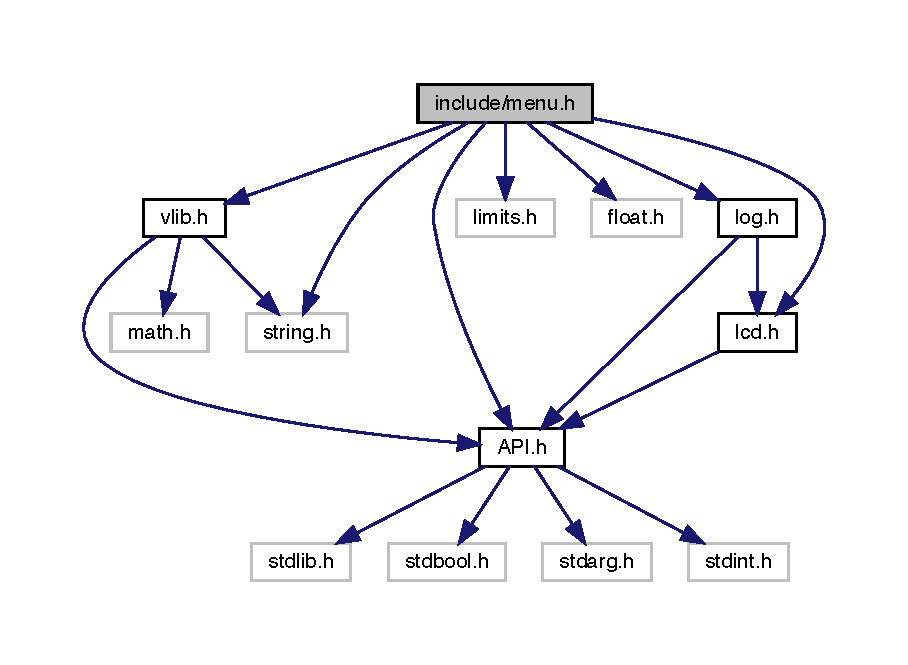
\includegraphics[width=350pt]{menu_8h__incl}
\end{center}
\end{figure}
This graph shows which files directly or indirectly include this file\+:\nopagebreak
\begin{figure}[H]
\begin{center}
\leavevmode
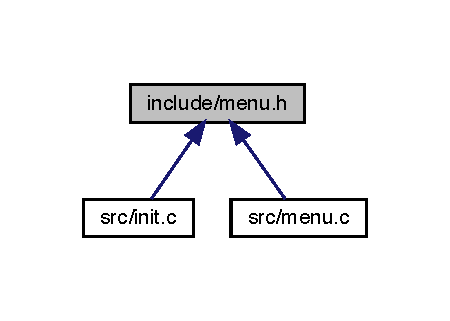
\includegraphics[width=216pt]{menu_8h__dep__incl}
\end{center}
\end{figure}
\subsection*{Data Structures}
\begin{DoxyCompactItemize}
\item 
struct \textbf{ menu\+\_\+t}
\begin{DoxyCompactList}\small\item\em Represents a specific instance of a menu. Will cause a memory leak if not deinitialized via denint\+\_\+menu. \end{DoxyCompactList}\end{DoxyCompactItemize}
\subsection*{Typedefs}
\begin{DoxyCompactItemize}
\item 
typedef struct \textbf{ menu\+\_\+t} \textbf{ menu\+\_\+t}
\begin{DoxyCompactList}\small\item\em Represents a specific instance of a menu. Will cause a memory leak if not deinitialized via denint\+\_\+menu. \end{DoxyCompactList}\end{DoxyCompactItemize}
\subsection*{Enumerations}
\begin{DoxyCompactItemize}
\item 
enum \textbf{ menu\+\_\+type} \{ \textbf{ I\+N\+T\+\_\+\+T\+Y\+PE}, 
\textbf{ F\+L\+O\+A\+T\+\_\+\+T\+Y\+PE}, 
\textbf{ S\+T\+R\+I\+N\+G\+\_\+\+T\+Y\+PE}
 \}\begin{DoxyCompactList}\small\item\em Represents the different types of menus. \end{DoxyCompactList}
\end{DoxyCompactItemize}
\subsection*{Functions}
\begin{DoxyCompactItemize}
\item 
static void \textbf{ calculate\+\_\+current\+\_\+display} (char $\ast$rtn, \textbf{ menu\+\_\+t} $\ast$menu)
\begin{DoxyCompactList}\small\item\em Static function that calculates the string from menu. \end{DoxyCompactList}\item 
static \textbf{ menu\+\_\+t} $\ast$ \textbf{ create\+\_\+menu} (enum \textbf{ menu\+\_\+type} type, const char $\ast$prompt)
\begin{DoxyCompactList}\small\item\em Static function that handles creation of menu. {\itshape  Menu must be freed or will cause memory leak {\itshape  }}\end{DoxyCompactList}\item 
void \textbf{ denint\+\_\+menu} (\textbf{ menu\+\_\+t} $\ast$menu)
\begin{DoxyCompactList}\small\item\em Destroys a menu {\itshape  Menu must be freed or will cause memory leak {\itshape  }}\end{DoxyCompactList}\item 
int \textbf{ display\+\_\+menu} (\textbf{ menu\+\_\+t} $\ast$menu)
\begin{DoxyCompactList}\small\item\em Displays a menu context, but does not display. {\itshape  Menu must be freed or will cause memory leak! {\itshape  Will exit if robot is enabled. This prevents menu from locking up system in even of a reset. }}\end{DoxyCompactList}\item 
\textbf{ menu\+\_\+t} $\ast$ \textbf{ init\+\_\+menu\+\_\+float} (enum \textbf{ menu\+\_\+type} type, float \textbf{ min}, float \textbf{ max}, float step, const char $\ast$prompt)
\begin{DoxyCompactList}\small\item\em Creates a menu context, but does not display. {\itshape  Menu must be freed or will cause memory leak! {\itshape  }}\end{DoxyCompactList}\item 
\textbf{ menu\+\_\+t} $\ast$ \textbf{ init\+\_\+menu\+\_\+int} (enum \textbf{ menu\+\_\+type} type, int \textbf{ min}, int \textbf{ max}, int step, const char $\ast$prompt)
\begin{DoxyCompactList}\small\item\em Creates a menu context, but does not display. {\itshape  Menu must be freed or will cause memory leak {\itshape  }}\end{DoxyCompactList}\item 
\textbf{ menu\+\_\+t} $\ast$ \textbf{ init\+\_\+menu\+\_\+var} (enum \textbf{ menu\+\_\+type} type, unsigned int nums, const char $\ast$prompt, char $\ast$options,...)
\begin{DoxyCompactList}\small\item\em Creates a menu context, but does not display. {\itshape  Menu must be freed or will cause memory leak {\itshape  }}\end{DoxyCompactList}\end{DoxyCompactItemize}


\subsection{Detailed Description}
Contains menu functionality and abstraction. 

\begin{DoxyAuthor}{Author}
Chris Jerrett 
\end{DoxyAuthor}
\begin{DoxyDate}{Date}
9/9/2017 
\end{DoxyDate}


Definition in file \textbf{ menu.\+h}.



\subsection{Typedef Documentation}
\mbox{\label{menu_8h_aac280f147a4bb94ab2f1a69eff76f751}} 
\index{menu.\+h@{menu.\+h}!menu\+\_\+t@{menu\+\_\+t}}
\index{menu\+\_\+t@{menu\+\_\+t}!menu.\+h@{menu.\+h}}
\subsubsection{menu\+\_\+t}
{\footnotesize\ttfamily typedef struct \textbf{ menu\+\_\+t}  \textbf{ menu\+\_\+t}}



Represents a specific instance of a menu. Will cause a memory leak if not deinitialized via denint\+\_\+menu. 

\begin{DoxyAuthor}{Author}
Chris Jerrett 
\end{DoxyAuthor}
\begin{DoxyDate}{Date}
9/8/17 
\end{DoxyDate}
\begin{DoxySeeAlso}{See also}
\doxyref{menu.\+h}{p.}{menu_8h} 

\doxyref{menu\+\_\+t}{p.}{structmenu__t} 

\doxyref{create\+\_\+menu}{p.}{menu_8c_aff4fd27ff7707295d91c67fa52a6b021} 

init\+\_\+menu 

\doxyref{display\+\_\+menu}{p.}{menu_8c_abfadedb104f89f672dd3045499975a71} 

\doxyref{menu\+\_\+type}{p.}{menu_8h_a6bbf4baf5018b0d76aab6c2e6bf85e62} 

\doxyref{denint\+\_\+menu}{p.}{menu_8c_a05a36619ac6c9ba4544eddb83ee2a50d} 
\end{DoxySeeAlso}


\subsection{Enumeration Type Documentation}
\mbox{\label{menu_8h_a6bbf4baf5018b0d76aab6c2e6bf85e62}} 
\index{menu.\+h@{menu.\+h}!menu\+\_\+type@{menu\+\_\+type}}
\index{menu\+\_\+type@{menu\+\_\+type}!menu.\+h@{menu.\+h}}
\subsubsection{menu\+\_\+type}
{\footnotesize\ttfamily enum \textbf{ menu\+\_\+type}}



Represents the different types of menus. 

\begin{DoxyAuthor}{Author}
Chris Jerrett 
\end{DoxyAuthor}
\begin{DoxyDate}{Date}
9/8/17 
\end{DoxyDate}
\begin{DoxySeeAlso}{See also}
\doxyref{menu.\+h}{p.}{menu_8h} 

\doxyref{menu\+\_\+t}{p.}{structmenu__t} 

\doxyref{create\+\_\+menu}{p.}{menu_8h_adcee778eac0edb821427d32949106dc5} 

init\+\_\+menu 

\doxyref{display\+\_\+menu}{p.}{menu_8h_abfadedb104f89f672dd3045499975a71} 

\doxyref{menu\+\_\+type}{p.}{menu_8h_a6bbf4baf5018b0d76aab6c2e6bf85e62} 
\end{DoxySeeAlso}
\begin{DoxyEnumFields}{Enumerator}
\raisebox{\heightof{T}}[0pt][0pt]{\index{I\+N\+T\+\_\+\+T\+Y\+PE@{I\+N\+T\+\_\+\+T\+Y\+PE}!menu.\+h@{menu.\+h}}\index{menu.\+h@{menu.\+h}!I\+N\+T\+\_\+\+T\+Y\+PE@{I\+N\+T\+\_\+\+T\+Y\+PE}}}\mbox{\label{menu_8h_a6bbf4baf5018b0d76aab6c2e6bf85e62a7fee88532b24b79bf2a88688a5d681d7}} 
I\+N\+T\+\_\+\+T\+Y\+PE&Menu type allowing user to select a integer. The integer type menu has a max, min and a step value. Each step is calculated. Will return the index of the selected value. Example\+: User goes forwards twice then it will return 2. \\
\hline

\raisebox{\heightof{T}}[0pt][0pt]{\index{F\+L\+O\+A\+T\+\_\+\+T\+Y\+PE@{F\+L\+O\+A\+T\+\_\+\+T\+Y\+PE}!menu.\+h@{menu.\+h}}\index{menu.\+h@{menu.\+h}!F\+L\+O\+A\+T\+\_\+\+T\+Y\+PE@{F\+L\+O\+A\+T\+\_\+\+T\+Y\+PE}}}\mbox{\label{menu_8h_a6bbf4baf5018b0d76aab6c2e6bf85e62ab2a272a88abadbaa481269e2506345c5}} 
F\+L\+O\+A\+T\+\_\+\+T\+Y\+PE&Menu type allowing user to select a float The float type menu has a max, min and a step value. Each step is calculated. Will return the index of the selected value. Example\+: User goes forwards twice then it will return 2. \\
\hline

\raisebox{\heightof{T}}[0pt][0pt]{\index{S\+T\+R\+I\+N\+G\+\_\+\+T\+Y\+PE@{S\+T\+R\+I\+N\+G\+\_\+\+T\+Y\+PE}!menu.\+h@{menu.\+h}}\index{menu.\+h@{menu.\+h}!S\+T\+R\+I\+N\+G\+\_\+\+T\+Y\+PE@{S\+T\+R\+I\+N\+G\+\_\+\+T\+Y\+PE}}}\mbox{\label{menu_8h_a6bbf4baf5018b0d76aab6c2e6bf85e62a7823190eb356a6edf2f33589f250053c}} 
S\+T\+R\+I\+N\+G\+\_\+\+T\+Y\+PE&Menu type allowing user to select a string from a array of strings. Will return the index of the selected value. Example\+: User goes forwards twice then it will return 2. \\
\hline

\end{DoxyEnumFields}


Definition at line \textbf{ 30} of file \textbf{ menu.\+h}.


\begin{DoxyCode}
00030                \{
00037   INT_TYPE,
00044   FLOAT_TYPE,
00050   STRING_TYPE
00051 \};
\end{DoxyCode}


\subsection{Function Documentation}
\mbox{\label{menu_8h_a0fb55c1213b23963d509b974d1254567}} 
\index{menu.\+h@{menu.\+h}!calculate\+\_\+current\+\_\+display@{calculate\+\_\+current\+\_\+display}}
\index{calculate\+\_\+current\+\_\+display@{calculate\+\_\+current\+\_\+display}!menu.\+h@{menu.\+h}}
\subsubsection{calculate\+\_\+current\+\_\+display()}
{\footnotesize\ttfamily static void calculate\+\_\+current\+\_\+display (\begin{DoxyParamCaption}\item[{char $\ast$}]{rtn,  }\item[{\textbf{ menu\+\_\+t} $\ast$}]{menu }\end{DoxyParamCaption})\hspace{0.3cm}{\ttfamily [static]}}



Static function that calculates the string from menu. 


\begin{DoxyParams}{Parameters}
{\em rtn} & the string to be written to \\
\hline
{\em menu} & the menu for prompt to be calculated from \\
\hline
\end{DoxyParams}
\begin{DoxyAuthor}{Author}
Chris Jerrett 
\end{DoxyAuthor}
\begin{DoxyDate}{Date}
9/8/17 
\end{DoxyDate}
\mbox{\label{menu_8h_adcee778eac0edb821427d32949106dc5}} 
\index{menu.\+h@{menu.\+h}!create\+\_\+menu@{create\+\_\+menu}}
\index{create\+\_\+menu@{create\+\_\+menu}!menu.\+h@{menu.\+h}}
\subsubsection{create\+\_\+menu()}
{\footnotesize\ttfamily static \textbf{ menu\+\_\+t}$\ast$ create\+\_\+menu (\begin{DoxyParamCaption}\item[{enum \textbf{ menu\+\_\+type}}]{type,  }\item[{const char $\ast$}]{prompt }\end{DoxyParamCaption})\hspace{0.3cm}{\ttfamily [static]}}



Static function that handles creation of menu. {\itshape  Menu must be freed or will cause memory leak {\itshape  }}

\begin{DoxyAuthor}{Author}
Chris Jerrett 
\end{DoxyAuthor}
\begin{DoxyDate}{Date}
9/8/17 
\end{DoxyDate}
\mbox{\label{menu_8h_a05a36619ac6c9ba4544eddb83ee2a50d}} 
\index{menu.\+h@{menu.\+h}!denint\+\_\+menu@{denint\+\_\+menu}}
\index{denint\+\_\+menu@{denint\+\_\+menu}!menu.\+h@{menu.\+h}}
\subsubsection{denint\+\_\+menu()}
{\footnotesize\ttfamily void denint\+\_\+menu (\begin{DoxyParamCaption}\item[{\textbf{ menu\+\_\+t} $\ast$}]{menu }\end{DoxyParamCaption})}



Destroys a menu {\itshape  Menu must be freed or will cause memory leak {\itshape  }}


\begin{DoxyParams}{Parameters}
{\em menu} & the menu to free \\
\hline
\end{DoxyParams}
\begin{DoxySeeAlso}{See also}
menu 
\end{DoxySeeAlso}
\begin{DoxyAuthor}{Author}
Chris Jerrett 
\end{DoxyAuthor}
\begin{DoxyDate}{Date}
9/8/17 
\end{DoxyDate}


Definition at line \textbf{ 163} of file \textbf{ menu.\+c}.



References \textbf{ menu\+\_\+t\+::options}, and \textbf{ menu\+\_\+t\+::prompt}.


\begin{DoxyCode}
00163                               \{
00164   free(menu->prompt);
00165   \textcolor{keywordflow}{if}(menu->options != NULL) free(menu->options);
00166   free(menu);
00167 \}
\end{DoxyCode}
\mbox{\label{menu_8h_abfadedb104f89f672dd3045499975a71}} 
\index{menu.\+h@{menu.\+h}!display\+\_\+menu@{display\+\_\+menu}}
\index{display\+\_\+menu@{display\+\_\+menu}!menu.\+h@{menu.\+h}}
\subsubsection{display\+\_\+menu()}
{\footnotesize\ttfamily int display\+\_\+menu (\begin{DoxyParamCaption}\item[{\textbf{ menu\+\_\+t} $\ast$}]{menu }\end{DoxyParamCaption})}



Displays a menu context, but does not display. {\itshape  Menu must be freed or will cause memory leak! {\itshape  Will exit if robot is enabled. This prevents menu from locking up system in even of a reset. }}


\begin{DoxyParams}{Parameters}
{\em menu} & the menu to display \\
\hline
\end{DoxyParams}
\begin{DoxySeeAlso}{See also}
\doxyref{menu\+\_\+type}{p.}{menu_8h_a6bbf4baf5018b0d76aab6c2e6bf85e62} 
\end{DoxySeeAlso}
\begin{DoxyAuthor}{Author}
Chris Jerrett 
\end{DoxyAuthor}
\begin{DoxyDate}{Date}
9/8/17 
\end{DoxyDate}


Definition at line \textbf{ 136} of file \textbf{ menu.\+c}.



References \textbf{ calculate\+\_\+current\+\_\+display()}, \textbf{ menu\+\_\+t\+::current}, \textbf{ lcd\+\_\+get\+\_\+pressed\+\_\+buttons()}, \textbf{ lcd\+\_\+print()}, \textbf{ P\+R\+E\+S\+S\+ED}, \textbf{ menu\+\_\+t\+::prompt}, \textbf{ R\+E\+L\+E\+A\+S\+ED}, and \textbf{ T\+O\+P\+\_\+\+R\+OW}.


\begin{DoxyCode}
00136                               \{
00137   lcd_print(TOP_ROW, menu->prompt);
00138   \textcolor{comment}{//Will exit if teleop or autonomous begin. This is extremely important if robot disconnects or resets.}
00139   \textcolor{keywordflow}{while}(lcd_get_pressed_buttons().middle == RELEASED && !isEnabled()) \{
00140     \textcolor{keywordtype}{char} val[16];
00141     calculate_current_display(val, menu);
00142 
00143     \textcolor{keywordflow}{if}(lcd_get_pressed_buttons().right == PRESSED) \{
00144       menu->current += 1;
00145     \}
00146     \textcolor{keywordflow}{if}(lcd_get_pressed_buttons().left == PRESSED) \{
00147       menu->current -= 1;
00148     \}
00149     delay(500);
00150   \}
00151   \textcolor{keywordflow}{return} menu->current;
00152 \}
\end{DoxyCode}
\mbox{\label{menu_8h_a5abb752733423805f59ef3b92e3c2e57}} 
\index{menu.\+h@{menu.\+h}!init\+\_\+menu\+\_\+float@{init\+\_\+menu\+\_\+float}}
\index{init\+\_\+menu\+\_\+float@{init\+\_\+menu\+\_\+float}!menu.\+h@{menu.\+h}}
\subsubsection{init\+\_\+menu\+\_\+float()}
{\footnotesize\ttfamily \textbf{ menu\+\_\+t}$\ast$ init\+\_\+menu\+\_\+float (\begin{DoxyParamCaption}\item[{enum \textbf{ menu\+\_\+type}}]{type,  }\item[{float}]{min,  }\item[{float}]{max,  }\item[{float}]{step,  }\item[{const char $\ast$}]{prompt }\end{DoxyParamCaption})}



Creates a menu context, but does not display. {\itshape  Menu must be freed or will cause memory leak! {\itshape  }}


\begin{DoxyParams}{Parameters}
{\em type} & the type of menu \\
\hline
\end{DoxyParams}
\begin{DoxySeeAlso}{See also}
\doxyref{menu\+\_\+type}{p.}{menu_8h_a6bbf4baf5018b0d76aab6c2e6bf85e62} 
\end{DoxySeeAlso}

\begin{DoxyParams}{Parameters}
{\em min} & the minimum value \\
\hline
{\em max} & the maximum value \\
\hline
{\em step} & the step value \\
\hline
{\em prompt} & the prompt to display to user \\
\hline
\end{DoxyParams}
\begin{DoxyAuthor}{Author}
Chris Jerrett 
\end{DoxyAuthor}
\begin{DoxyDate}{Date}
9/8/17 
\end{DoxyDate}


Definition at line \textbf{ 92} of file \textbf{ menu.\+c}.



References \textbf{ create\+\_\+menu()}, \textbf{ max()}, \textbf{ menu\+\_\+t\+::max\+\_\+f}, \textbf{ min()}, \textbf{ menu\+\_\+t\+::min\+\_\+f}, and \textbf{ menu\+\_\+t\+::step\+\_\+f}.


\begin{DoxyCode}
00092                                                                                                   \{
00093   menu_t* menu = create_menu(type, prompt);
00094   menu->min_f = min;
00095   menu->max_f = max;
00096   menu->step_f = step;
00097   \textcolor{keywordflow}{return} menu;
00098 \}
\end{DoxyCode}
\mbox{\label{menu_8h_ac8efedba760ec35ebf841ab19543ba5a}} 
\index{menu.\+h@{menu.\+h}!init\+\_\+menu\+\_\+int@{init\+\_\+menu\+\_\+int}}
\index{init\+\_\+menu\+\_\+int@{init\+\_\+menu\+\_\+int}!menu.\+h@{menu.\+h}}
\subsubsection{init\+\_\+menu\+\_\+int()}
{\footnotesize\ttfamily \textbf{ menu\+\_\+t}$\ast$ init\+\_\+menu\+\_\+int (\begin{DoxyParamCaption}\item[{enum \textbf{ menu\+\_\+type}}]{type,  }\item[{int}]{min,  }\item[{int}]{max,  }\item[{int}]{step,  }\item[{const char $\ast$}]{prompt }\end{DoxyParamCaption})}



Creates a menu context, but does not display. {\itshape  Menu must be freed or will cause memory leak {\itshape  }}


\begin{DoxyParams}{Parameters}
{\em type} & the type of menu \\
\hline
\end{DoxyParams}
\begin{DoxySeeAlso}{See also}
\doxyref{menu\+\_\+type}{p.}{menu_8h_a6bbf4baf5018b0d76aab6c2e6bf85e62} 
\end{DoxySeeAlso}

\begin{DoxyParams}{Parameters}
{\em min} & the minimum value \\
\hline
{\em max} & the maximum value \\
\hline
{\em step} & the step value \\
\hline
{\em prompt} & the prompt to display to user \\
\hline
\end{DoxyParams}
\begin{DoxyAuthor}{Author}
Chris Jerrett 
\end{DoxyAuthor}
\begin{DoxyDate}{Date}
9/8/17 
\end{DoxyDate}


Definition at line \textbf{ 71} of file \textbf{ menu.\+c}.



References \textbf{ create\+\_\+menu()}, \textbf{ max()}, \textbf{ menu\+\_\+t\+::max}, \textbf{ min()}, \textbf{ menu\+\_\+t\+::min}, and \textbf{ menu\+\_\+t\+::step}.


\begin{DoxyCode}
00071                                                                                           \{
00072   menu_t* menu = create_menu(type, prompt);
00073   menu->min = min;
00074   menu->max = max;
00075   menu->step = step;
00076   \textcolor{keywordflow}{return} menu;
00077 \}
\end{DoxyCode}
\mbox{\label{menu_8h_a3529988b0a7c12cb3f2ebb3cf5595594}} 
\index{menu.\+h@{menu.\+h}!init\+\_\+menu\+\_\+var@{init\+\_\+menu\+\_\+var}}
\index{init\+\_\+menu\+\_\+var@{init\+\_\+menu\+\_\+var}!menu.\+h@{menu.\+h}}
\subsubsection{init\+\_\+menu\+\_\+var()}
{\footnotesize\ttfamily \textbf{ menu\+\_\+t}$\ast$ init\+\_\+menu\+\_\+var (\begin{DoxyParamCaption}\item[{enum \textbf{ menu\+\_\+type}}]{type,  }\item[{unsigned int}]{nums,  }\item[{const char $\ast$}]{prompt,  }\item[{char $\ast$}]{options,  }\item[{}]{... }\end{DoxyParamCaption})}



Creates a menu context, but does not display. {\itshape  Menu must be freed or will cause memory leak {\itshape  }}


\begin{DoxyParams}{Parameters}
{\em type} & the type of menu \\
\hline
\end{DoxyParams}
\begin{DoxySeeAlso}{See also}
\doxyref{menu\+\_\+type}{p.}{menu_8h_a6bbf4baf5018b0d76aab6c2e6bf85e62} 
\end{DoxySeeAlso}

\begin{DoxyParams}{Parameters}
{\em nums} & the number of elements passed to function \\
\hline
{\em prompt} & the prompt to display to user \\
\hline
{\em options} & the options to display for user \\
\hline
\end{DoxyParams}
\begin{DoxyAuthor}{Author}
Chris Jerrett 
\end{DoxyAuthor}
\begin{DoxyDate}{Date}
9/8/17 
\end{DoxyDate}


Definition at line \textbf{ 44} of file \textbf{ menu.\+c}.



References \textbf{ create\+\_\+menu()}, \textbf{ menu\+\_\+t\+::length}, and \textbf{ menu\+\_\+t\+::options}.


\begin{DoxyCode}
00044                                                                                                     \{
00045   menu_t* menu = create_menu(type, prompt);
00046   va\_list values;
00047   \textcolor{keywordtype}{char} **options\_array = (\textcolor{keywordtype}{char}**)calloc(\textcolor{keyword}{sizeof}(\textcolor{keywordtype}{char}*), nums);
00048   va\_start(values, options);
00049   \textcolor{keywordflow}{for}(\textcolor{keywordtype}{unsigned} \textcolor{keywordtype}{int} i = 0; i < nums; i++)\{
00050     options\_array[i] = va\_arg(values, \textcolor{keywordtype}{char}*);
00051   \}
00052   va\_end(values);
00053   menu->options = options\_array;
00054   menu->length = nums;
00055   \textcolor{keywordflow}{return} menu;
00056 \}
\end{DoxyCode}

\hypertarget{ports_8h}{}\section{include/ports.h File Reference}
\label{ports_8h}\index{include/ports.\+h@{include/ports.\+h}}
\subsection*{Macros}
\begin{DoxyCompactItemize}
\item 
\#define \hyperlink{ports_8h_ae59fbcf599f31d0317338ee35491c175}{I\+M\+E\+\_\+\+F\+R\+O\+N\+T\+\_\+\+R\+I\+G\+HT}~0
\end{DoxyCompactItemize}


\subsection{Macro Definition Documentation}
\mbox{\Hypertarget{ports_8h_ae59fbcf599f31d0317338ee35491c175}\label{ports_8h_ae59fbcf599f31d0317338ee35491c175}} 
\index{ports.\+h@{ports.\+h}!I\+M\+E\+\_\+\+F\+R\+O\+N\+T\+\_\+\+R\+I\+G\+HT@{I\+M\+E\+\_\+\+F\+R\+O\+N\+T\+\_\+\+R\+I\+G\+HT}}
\index{I\+M\+E\+\_\+\+F\+R\+O\+N\+T\+\_\+\+R\+I\+G\+HT@{I\+M\+E\+\_\+\+F\+R\+O\+N\+T\+\_\+\+R\+I\+G\+HT}!ports.\+h@{ports.\+h}}
\subsubsection{\texorpdfstring{I\+M\+E\+\_\+\+F\+R\+O\+N\+T\+\_\+\+R\+I\+G\+HT}{IME\_FRONT\_RIGHT}}
{\footnotesize\ttfamily \#define I\+M\+E\+\_\+\+F\+R\+O\+N\+T\+\_\+\+R\+I\+G\+HT~0}



Definition at line 4 of file ports.\+h.


\subsection{include/vmath.h File Reference}
\label{vmath_8h}\index{include/vmath.\+h@{include/vmath.\+h}}


Vex Specific Math Functions, includes\+: Cartesian to polar cordinates.  


{\ttfamily \#include $<$math.\+h$>$}\newline
\subsubsection*{Data Structures}
\begin{DoxyCompactItemize}
\item 
struct \textbf{ cord}
\begin{DoxyCompactList}\small\item\em A struct that contains cartesian coordinates. \end{DoxyCompactList}\item 
struct \textbf{ polar\+\_\+cord}
\begin{DoxyCompactList}\small\item\em A struct that contains polar coordinates. \end{DoxyCompactList}\end{DoxyCompactItemize}
\subsubsection*{Macros}
\begin{DoxyCompactItemize}
\item 
\#define \textbf{ M\+\_\+\+PI}~3.\+14159265358979323846
\end{DoxyCompactItemize}
\subsubsection*{Functions}
\begin{DoxyCompactItemize}
\item 
struct \textbf{ polar\+\_\+cord} \textbf{ cartesian\+\_\+cord\+\_\+to\+\_\+polar} (struct \textbf{ cord} cords)
\begin{DoxyCompactList}\small\item\em Function to convert x and y 2 dimensional cartesian cordinated to polar coordinates. \end{DoxyCompactList}\item 
struct \textbf{ polar\+\_\+cord} \textbf{ cartesian\+\_\+to\+\_\+polar} (float x, float y)
\begin{DoxyCompactList}\small\item\em Function to convert x and y 2 dimensional cartesian coordinated to polar coordinates. \end{DoxyCompactList}\item 
int \textbf{ max} (int a, int b)
\begin{DoxyCompactList}\small\item\em the min of two values \end{DoxyCompactList}\item 
int \textbf{ min} (int a, int b)
\begin{DoxyCompactList}\small\item\em the min of two values \end{DoxyCompactList}\item 
double \textbf{ sind} (double angle)
\begin{DoxyCompactList}\small\item\em sine of a angle in degrees \end{DoxyCompactList}\end{DoxyCompactItemize}


\subsubsection{Detailed Description}
Vex Specific Math Functions, includes\+: Cartesian to polar cordinates. 

\begin{DoxyAuthor}{Author}
Christian Desimone 

Chris Jerrett 
\end{DoxyAuthor}
\begin{DoxyDate}{Date}
9/9/2017 
\end{DoxyDate}


Definition in file \textbf{ vmath.\+h}.



\subsubsection{Macro Definition Documentation}
\mbox{\label{vmath_8h_ae71449b1cc6e6250b91f539153a7a0d3}} 
\index{vmath.\+h@{vmath.\+h}!M\+\_\+\+PI@{M\+\_\+\+PI}}
\index{M\+\_\+\+PI@{M\+\_\+\+PI}!vmath.\+h@{vmath.\+h}}
\paragraph{M\+\_\+\+PI}
{\footnotesize\ttfamily \#define M\+\_\+\+PI~3.\+14159265358979323846}



Definition at line \textbf{ 13} of file \textbf{ vmath.\+h}.



Referenced by \textbf{ calculate\+\_\+encoder\+\_\+odemetry()}, and \textbf{ sind()}.



\subsubsection{Function Documentation}
\mbox{\label{vmath_8h_a832105cf858b3046c57c0d08a4e7c38b}} 
\index{vmath.\+h@{vmath.\+h}!cartesian\+\_\+cord\+\_\+to\+\_\+polar@{cartesian\+\_\+cord\+\_\+to\+\_\+polar}}
\index{cartesian\+\_\+cord\+\_\+to\+\_\+polar@{cartesian\+\_\+cord\+\_\+to\+\_\+polar}!vmath.\+h@{vmath.\+h}}
\paragraph{cartesian\+\_\+cord\+\_\+to\+\_\+polar()}
{\footnotesize\ttfamily struct \textbf{ polar\+\_\+cord} cartesian\+\_\+cord\+\_\+to\+\_\+polar (\begin{DoxyParamCaption}\item[{struct \textbf{ cord}}]{cords }\end{DoxyParamCaption})}



Function to convert x and y 2 dimensional cartesian cordinated to polar coordinates. 

\begin{DoxyAuthor}{Author}
Christian Desimone 
\end{DoxyAuthor}
\begin{DoxyDate}{Date}
9/8/2017
\end{DoxyDate}

\begin{DoxyParams}{Parameters}
{\em cords} & the cartesian cords \\
\hline
\end{DoxyParams}
\begin{DoxyReturn}{Returns}
a struct containing the angle and magnitude. 
\end{DoxyReturn}
\begin{DoxySeeAlso}{See also}
\doxyref{polar\+\_\+cord}{p.}{structpolar__cord} 

\doxyref{cord}{p.}{structcord} 
\end{DoxySeeAlso}


Definition at line \textbf{ 53} of file \textbf{ vmath.\+c}.



References \textbf{ cartesian\+\_\+to\+\_\+polar()}.

\mbox{\label{vmath_8h_a1c4a1747b714f5d4654f0614193f9e49}} 
\index{vmath.\+h@{vmath.\+h}!cartesian\+\_\+to\+\_\+polar@{cartesian\+\_\+to\+\_\+polar}}
\index{cartesian\+\_\+to\+\_\+polar@{cartesian\+\_\+to\+\_\+polar}!vmath.\+h@{vmath.\+h}}
\paragraph{cartesian\+\_\+to\+\_\+polar()}
{\footnotesize\ttfamily struct \textbf{ polar\+\_\+cord} cartesian\+\_\+to\+\_\+polar (\begin{DoxyParamCaption}\item[{float}]{x,  }\item[{float}]{y }\end{DoxyParamCaption})}



Function to convert x and y 2 dimensional cartesian coordinated to polar coordinates. 

\begin{DoxyAuthor}{Author}
Christian Desimone 
\end{DoxyAuthor}
\begin{DoxyDate}{Date}
9/8/2017
\end{DoxyDate}

\begin{DoxyParams}{Parameters}
{\em x} & float value of the x cartesian coordinate. \\
\hline
{\em y} & float value of the y cartesian coordinate. \\
\hline
\end{DoxyParams}
\begin{DoxyReturn}{Returns}
a struct containing the angle and magnitude. 
\end{DoxyReturn}
\begin{DoxySeeAlso}{See also}
\doxyref{polar\+\_\+cord}{p.}{structpolar__cord} 
\end{DoxySeeAlso}


Definition at line \textbf{ 15} of file \textbf{ vmath.\+c}.



References \textbf{ polar\+\_\+cord\+::angle}, and \textbf{ polar\+\_\+cord\+::magnitue}.



Referenced by \textbf{ cartesian\+\_\+cord\+\_\+to\+\_\+polar()}.

\mbox{\label{vmath_8h_af082905f7eac6d03e92015146bbc1925}} 
\index{vmath.\+h@{vmath.\+h}!max@{max}}
\index{max@{max}!vmath.\+h@{vmath.\+h}}
\paragraph{max()}
{\footnotesize\ttfamily int max (\begin{DoxyParamCaption}\item[{int}]{a,  }\item[{int}]{b }\end{DoxyParamCaption})}



the min of two values 


\begin{DoxyParams}{Parameters}
{\em a} & the first \\
\hline
{\em b} & the second \\
\hline
\end{DoxyParams}
\begin{DoxyReturn}{Returns}
the smaller of a and b 
\end{DoxyReturn}


Definition at line \textbf{ 83} of file \textbf{ vmath.\+c}.



Referenced by \textbf{ calculate\+\_\+current\+\_\+display()}, \textbf{ init\+\_\+menu\+\_\+float()}, and \textbf{ init\+\_\+menu\+\_\+int()}.

\mbox{\label{vmath_8h_abd8bbcfabb3ddef2ccaafb9928a37b95}} 
\index{vmath.\+h@{vmath.\+h}!min@{min}}
\index{min@{min}!vmath.\+h@{vmath.\+h}}
\paragraph{min()}
{\footnotesize\ttfamily int min (\begin{DoxyParamCaption}\item[{int}]{a,  }\item[{int}]{b }\end{DoxyParamCaption})}



the min of two values 


\begin{DoxyParams}{Parameters}
{\em a} & the first \\
\hline
{\em b} & the second \\
\hline
\end{DoxyParams}
\begin{DoxyReturn}{Returns}
the smaller of a and b 
\end{DoxyReturn}


Definition at line \textbf{ 71} of file \textbf{ vmath.\+c}.



Referenced by \textbf{ calculate\+\_\+current\+\_\+display()}, \textbf{ init\+\_\+menu\+\_\+float()}, and \textbf{ init\+\_\+menu\+\_\+int()}.

\mbox{\label{vmath_8h_a2b83ceb814c90ebfa042a26d884ac159}} 
\index{vmath.\+h@{vmath.\+h}!sind@{sind}}
\index{sind@{sind}!vmath.\+h@{vmath.\+h}}
\paragraph{sind()}
{\footnotesize\ttfamily double sind (\begin{DoxyParamCaption}\item[{double}]{angle }\end{DoxyParamCaption})}



sine of a angle in degrees 



Definition at line \textbf{ 60} of file \textbf{ vmath.\+c}.



References \textbf{ M\+\_\+\+PI}.


\subsection{R\+E\+A\+D\+M\+E.\+md File Reference}
\label{_r_e_a_d_m_e_8md}\index{R\+E\+A\+D\+M\+E.\+md@{R\+E\+A\+D\+M\+E.\+md}}

\hypertarget{auto_8c}{}\section{src/auto.c File Reference}
\label{auto_8c}\index{src/auto.\+c@{src/auto.\+c}}


File for autonomous code.  


{\ttfamily \#include \char`\"{}main.\+h\char`\"{}}\newline
\subsection*{Functions}
\begin{DoxyCompactItemize}
\item 
void \hyperlink{auto_8c_a3c7ca506bbc071fa740de13805b7f376}{autonomous} ()
\end{DoxyCompactItemize}


\subsection{Detailed Description}
File for autonomous code. 

This file should contain the user \hyperlink{auto_8c_a3c7ca506bbc071fa740de13805b7f376}{autonomous()} function and any functions related to it.

Any copyright is dedicated to the Public Domain. \href{http://creativecommons.org/publicdomain/zero/1.0/}{\tt http\+://creativecommons.\+org/publicdomain/zero/1.\+0/}

P\+R\+OS contains Free\+R\+T\+OS (\href{http://www.freertos.org}{\tt http\+://www.\+freertos.\+org}) whose source code may be obtained from \href{http://sourceforge.net/projects/freertos/files/}{\tt http\+://sourceforge.\+net/projects/freertos/files/} or on request. 

\subsection{Function Documentation}
\mbox{\Hypertarget{auto_8c_a3c7ca506bbc071fa740de13805b7f376}\label{auto_8c_a3c7ca506bbc071fa740de13805b7f376}} 
\index{auto.\+c@{auto.\+c}!autonomous@{autonomous}}
\index{autonomous@{autonomous}!auto.\+c@{auto.\+c}}
\subsubsection{\texorpdfstring{autonomous()}{autonomous()}}
{\footnotesize\ttfamily void autonomous (\begin{DoxyParamCaption}{ }\end{DoxyParamCaption})}

Runs the user autonomous code. This function will be started in its own task with the default priority and stack size whenever the robot is enabled via the Field Management System or the V\+EX Competition Switch in the autonomous mode. If the robot is disabled or communications is lost, the autonomous task will be stopped by the kernel. Re-\/enabling the robot will restart the task, not re-\/start it from where it left off.

Code running in the autonomous task cannot access information from the V\+EX Joystick. However, the autonomous function can be invoked from another task if a V\+EX Competition Switch is not available, and it can access joystick information if called in this way.

The autonomous task may exit, unlike \hyperlink{main_8h_ac71a94af413917f27d108e95c4d6f6a7}{operator\+Control()} which should never exit. If it does so, the robot will await a switch to another mode or disable/enable cycle. 
\subsection{src/drive.c File Reference}
\label{drive_8c}\index{src/drive.\+c@{src/drive.\+c}}
\subsubsection*{Functions}
\begin{DoxyCompactItemize}
\item 
int \textbf{ get\+Thresh} ()
\begin{DoxyCompactList}\small\item\em Gets the deadzone threshhold on the joystick. \end{DoxyCompactList}\item 
static float \textbf{ joystick\+Exp} (int joystick\+Val)
\begin{DoxyCompactList}\small\item\em Applies exponential scale to a joystick value. \end{DoxyCompactList}\item 
void \textbf{ set\+\_\+side\+\_\+speed} (\textbf{ side\+\_\+t} \textbf{ side}, int speed)
\begin{DoxyCompactList}\small\item\em sets the speed of one side of the robot. \end{DoxyCompactList}\item 
void \textbf{ set\+Thresh} (int t)
\begin{DoxyCompactList}\small\item\em Sets the deadzone threshhold on the joystick. \end{DoxyCompactList}\item 
void \textbf{ update\+\_\+drive\+\_\+motors} ()
\begin{DoxyCompactList}\small\item\em Updates the drive motors during teleop. \end{DoxyCompactList}\end{DoxyCompactItemize}
\subsubsection*{Variables}
\begin{DoxyCompactItemize}
\item 
static int \textbf{ thresh} = 10
\end{DoxyCompactItemize}


\subsubsection{Function Documentation}
\mbox{\label{drive_8c_a9caa5e772598f9182c9ec84cf8c351ee}} 
\index{drive.\+c@{drive.\+c}!get\+Thresh@{get\+Thresh}}
\index{get\+Thresh@{get\+Thresh}!drive.\+c@{drive.\+c}}
\paragraph{get\+Thresh()}
{\footnotesize\ttfamily int get\+Thresh (\begin{DoxyParamCaption}{ }\end{DoxyParamCaption})}



Gets the deadzone threshhold on the joystick. 

\begin{DoxyAuthor}{Author}
Christian Desimone 
\end{DoxyAuthor}


Definition at line \textbf{ 12} of file \textbf{ drive.\+c}.



References \textbf{ thresh}.


\begin{DoxyCode}
00012 \{ \textcolor{keywordflow}{return} thresh; \}
\end{DoxyCode}
\mbox{\label{drive_8c_a6de4fbb9197f2f350c53a9f8bf23a8f1}} 
\index{drive.\+c@{drive.\+c}!joystick\+Exp@{joystick\+Exp}}
\index{joystick\+Exp@{joystick\+Exp}!drive.\+c@{drive.\+c}}
\paragraph{joystick\+Exp()}
{\footnotesize\ttfamily static float joystick\+Exp (\begin{DoxyParamCaption}\item[{int}]{joystick\+Val }\end{DoxyParamCaption})\hspace{0.3cm}{\ttfamily [static]}}



Applies exponential scale to a joystick value. 

\begin{DoxyAuthor}{Author}
Christian De\+Simone, Chris Jerrett 
\end{DoxyAuthor}

\begin{DoxyParams}{Parameters}
{\em joystick\+Val} & the analog value from the joystick \\
\hline
\end{DoxyParams}
\begin{DoxyDate}{Date}
9/21/2017 
\end{DoxyDate}


Definition at line \textbf{ 73} of file \textbf{ drive.\+c}.



References \textbf{ thresh}.


\begin{DoxyCode}
00073                                           \{
00074   \textcolor{comment}{// make the offset negative if moving backwards}
00075   \textcolor{keywordflow}{if} (abs(joystickVal) < thresh) \{
00076     \textcolor{keywordflow}{return} 0;
00077   \}
00078 
00079   \textcolor{keywordtype}{int} offset;
00080   \textcolor{comment}{// Use the threshold to ensure the joystick values are significant}
00081   \textcolor{keywordflow}{if} (joystickVal < 0) \{
00082     offset = -(thresh);
00083   \} \textcolor{keywordflow}{else} \{
00084     offset = thresh;
00085   \}
00086   \textcolor{comment}{// Apply the function ((((x/10)^3)/18) + offset) * 0.8 to the joystick value}
00087   \textcolor{keywordflow}{return} (pow(joystickVal / 10, 3) / 18 + offset) * 0.8;
00088 \}
\end{DoxyCode}
\mbox{\label{drive_8c_a8df41fd50094c065eedc81fc5e6595d1}} 
\index{drive.\+c@{drive.\+c}!set\+\_\+side\+\_\+speed@{set\+\_\+side\+\_\+speed}}
\index{set\+\_\+side\+\_\+speed@{set\+\_\+side\+\_\+speed}!drive.\+c@{drive.\+c}}
\paragraph{set\+\_\+side\+\_\+speed()}
{\footnotesize\ttfamily void set\+\_\+side\+\_\+speed (\begin{DoxyParamCaption}\item[{\textbf{ side\+\_\+t}}]{side,  }\item[{int}]{speed }\end{DoxyParamCaption})}



sets the speed of one side of the robot. 

\begin{DoxyAuthor}{Author}
Christian Desimone 
\end{DoxyAuthor}

\begin{DoxyParams}{Parameters}
{\em side} & a side enum which indicates the size. \\
\hline
{\em speed} & the speed of the side. Can range from -\/127 -\/ 127 negative being back and positive forwards \\
\hline
\end{DoxyParams}


Definition at line \textbf{ 54} of file \textbf{ drive.\+c}.



References \textbf{ B\+O\+TH}, \textbf{ L\+E\+FT}, \textbf{ R\+I\+G\+HT}, and \textbf{ set\+\_\+motor\+\_\+slew()}.



Referenced by \textbf{ auton\+\_\+drive\+\_\+towards\+\_\+mobile\+\_\+goal()}, \textbf{ auton\+\_\+turn\+\_\+180()}, \textbf{ autonomous()}, and \textbf{ update\+\_\+drive\+\_\+motors()}.


\begin{DoxyCode}
00054                                             \{
00055   \textcolor{keywordflow}{if} (side == RIGHT || side == BOTH) \{
00056     set_motor_slew(MOTOR\_BACK\_RIGHT, -speed);
00057     set_motor_slew(MOTOR\_FRONT\_RIGHT, -speed);
00058     set_motor_slew(MOTOR\_MIDDLE\_RIGHT, -speed);
00059   \}
00060   \textcolor{keywordflow}{if} (side == LEFT || side == BOTH) \{
00061     set_motor_slew(MOTOR\_BACK\_LEFT, speed);
00062     set_motor_slew(MOTOR\_MIDDLE\_LEFT, speed);
00063     set_motor_slew(MOTOR\_FRONT\_LEFT, speed);
00064   \}
00065 \}
\end{DoxyCode}
Here is the call graph for this function\+:
\nopagebreak
\begin{figure}[H]
\begin{center}
\leavevmode
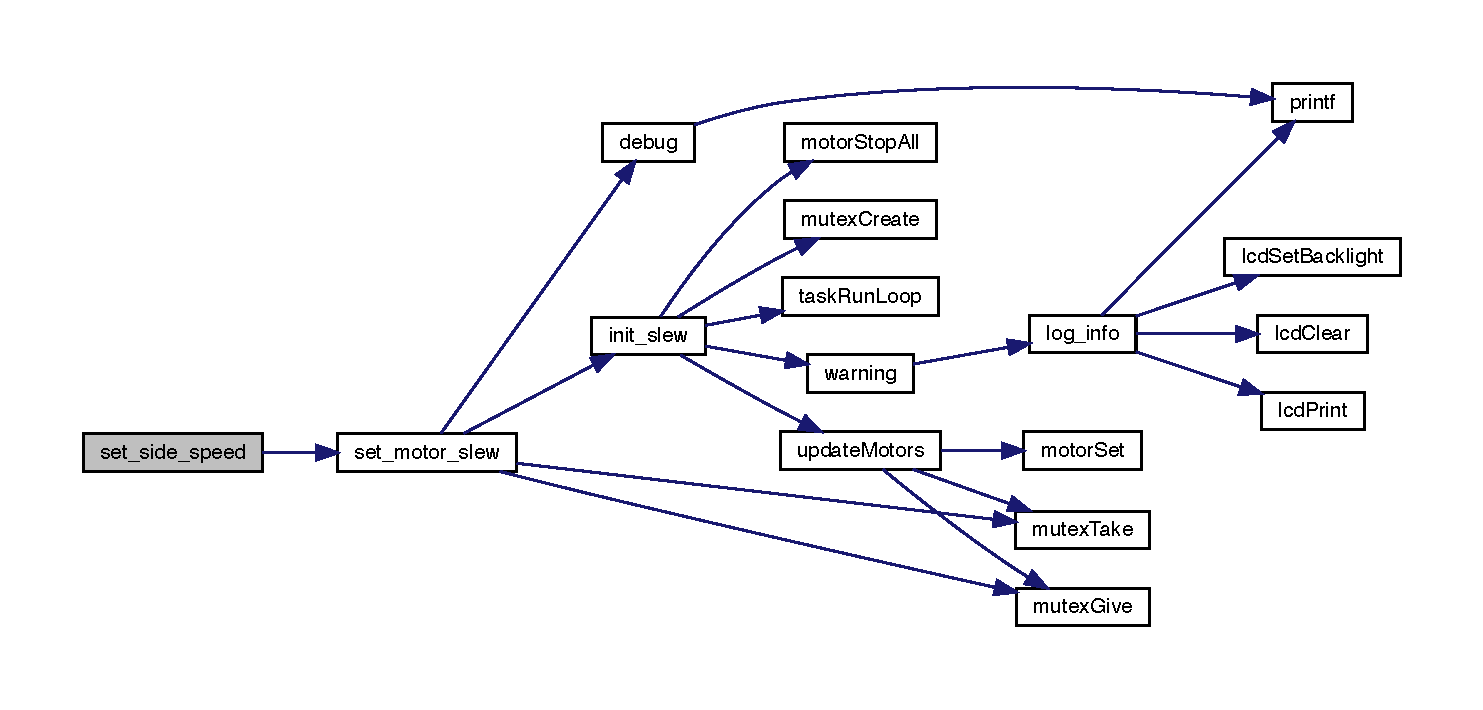
\includegraphics[width=350pt]{drive_8c_a8df41fd50094c065eedc81fc5e6595d1_cgraph}
\end{center}
\end{figure}
Here is the caller graph for this function\+:
\nopagebreak
\begin{figure}[H]
\begin{center}
\leavevmode
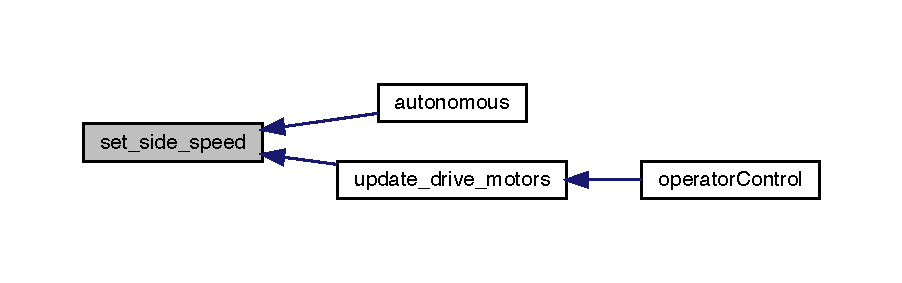
\includegraphics[width=350pt]{drive_8c_a8df41fd50094c065eedc81fc5e6595d1_icgraph}
\end{center}
\end{figure}
\mbox{\label{drive_8c_a53d6e35d53ec3e0b1b1c489d8203f204}} 
\index{drive.\+c@{drive.\+c}!set\+Thresh@{set\+Thresh}}
\index{set\+Thresh@{set\+Thresh}!drive.\+c@{drive.\+c}}
\paragraph{set\+Thresh()}
{\footnotesize\ttfamily void set\+Thresh (\begin{DoxyParamCaption}\item[{int}]{t }\end{DoxyParamCaption})}



Sets the deadzone threshhold on the joystick. 

Sets the deadzone threshhold on the drive.

\begin{DoxyAuthor}{Author}
Christian Desimone 
\end{DoxyAuthor}


Definition at line \textbf{ 18} of file \textbf{ drive.\+c}.



References \textbf{ thresh}.


\begin{DoxyCode}
00018 \{ thresh = t; \}
\end{DoxyCode}
\mbox{\label{drive_8c_a8224a4626a934d30ed587671b7004bf8}} 
\index{drive.\+c@{drive.\+c}!update\+\_\+drive\+\_\+motors@{update\+\_\+drive\+\_\+motors}}
\index{update\+\_\+drive\+\_\+motors@{update\+\_\+drive\+\_\+motors}!drive.\+c@{drive.\+c}}
\paragraph{update\+\_\+drive\+\_\+motors()}
{\footnotesize\ttfamily void update\+\_\+drive\+\_\+motors (\begin{DoxyParamCaption}{ }\end{DoxyParamCaption})}



Updates the drive motors during teleop. 

\begin{DoxyAuthor}{Author}
Christian Desimone 
\end{DoxyAuthor}
\begin{DoxyDate}{Date}
9/5/17 
\end{DoxyDate}


Definition at line \textbf{ 25} of file \textbf{ drive.\+c}.



References \textbf{ joystick\+Get\+Analog()}, \textbf{ L\+E\+FT}, \textbf{ R\+I\+G\+HT}, \textbf{ set\+\_\+side\+\_\+speed()}, \textbf{ thresh}, \textbf{ cord\+::x}, and \textbf{ cord\+::y}.



Referenced by \textbf{ operator\+Control()}.


\begin{DoxyCode}
00025                            \{
00026   \textcolor{comment}{// Get the joystick values from the controller}
00027   \textcolor{keywordtype}{int} x = 0;
00028   \textcolor{keywordtype}{int} y = 0;
00029   x = -(joystickGetAnalog(MASTER, 3));
00030   y = (joystickGetAnalog(MASTER, 1));
00031   \textcolor{comment}{// Make sure the joystick values are significant enough to change the motors}
00032   \textcolor{keywordflow}{if} (x < thresh && x > -thresh) \{
00033     x = 0;
00034   \}
00035   \textcolor{keywordflow}{if} (y < thresh && y > -thresh) \{
00036     y = 0;
00037   \}
00038   \textcolor{comment}{// Create motor values for the left and right from the x and y of the joystick}
00039   \textcolor{keywordtype}{int} r = (x + y);
00040   \textcolor{keywordtype}{int} l = -(x - y);
00041 
00042   \textcolor{comment}{// Set the drive motors}
00043   set_side_speed(LEFT, l);
00044   set_side_speed(RIGHT, -r);
00045 \}
\end{DoxyCode}
Here is the call graph for this function\+:
\nopagebreak
\begin{figure}[H]
\begin{center}
\leavevmode
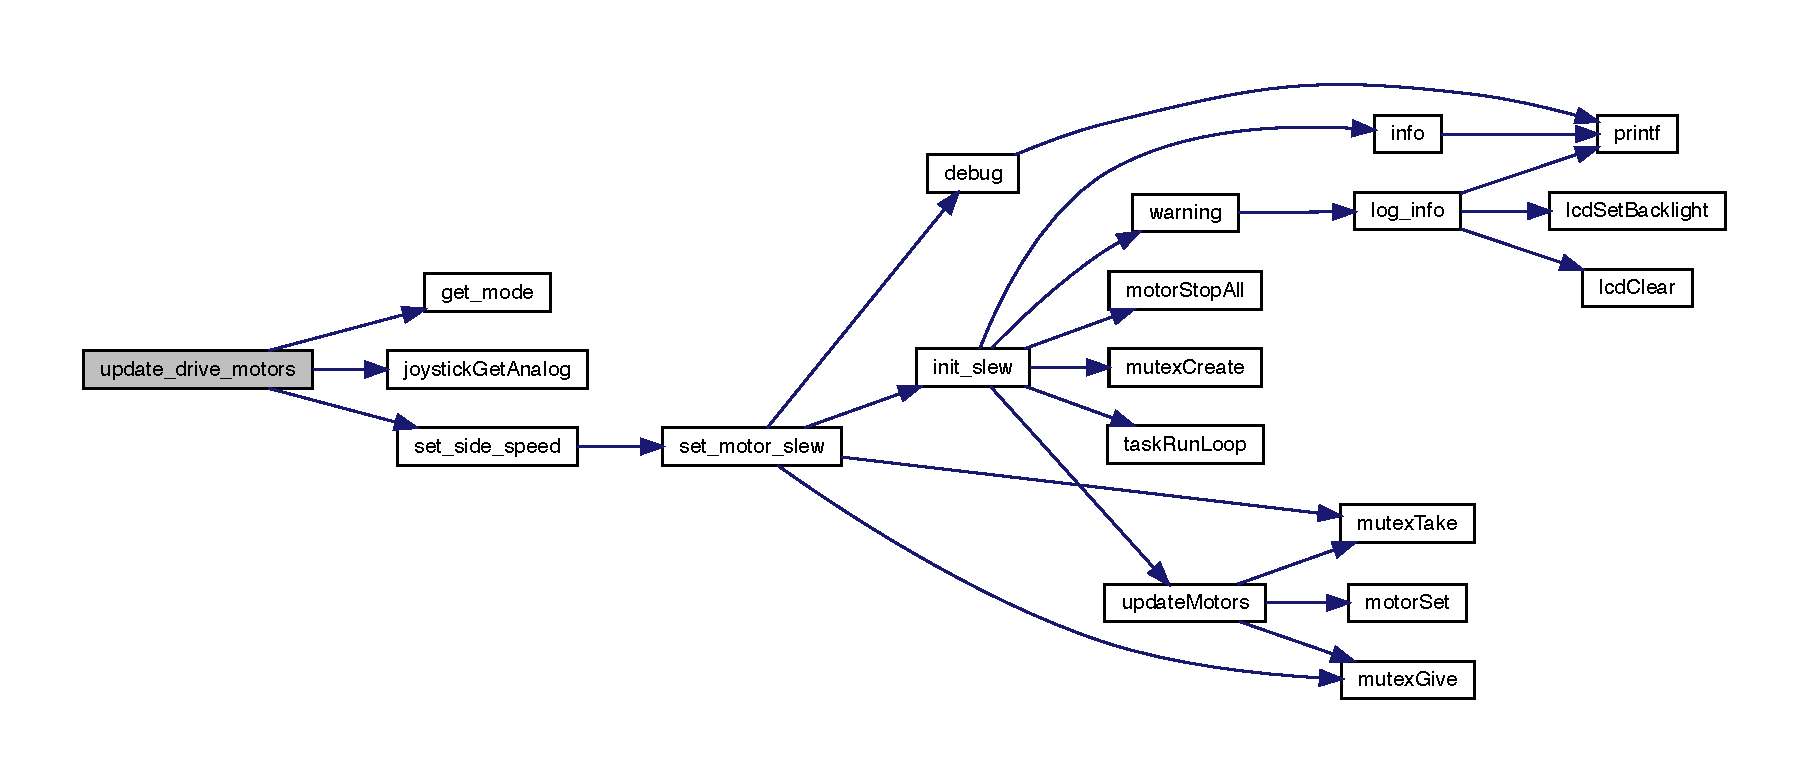
\includegraphics[width=350pt]{drive_8c_a8224a4626a934d30ed587671b7004bf8_cgraph}
\end{center}
\end{figure}
Here is the caller graph for this function\+:
\nopagebreak
\begin{figure}[H]
\begin{center}
\leavevmode
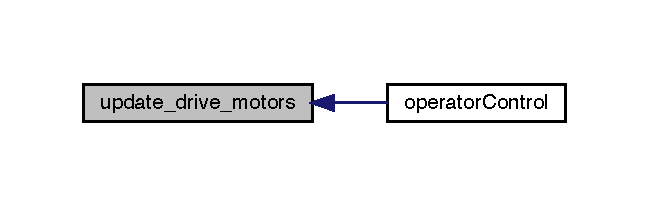
\includegraphics[width=311pt]{drive_8c_a8224a4626a934d30ed587671b7004bf8_icgraph}
\end{center}
\end{figure}


\subsubsection{Variable Documentation}
\mbox{\label{drive_8c_a6cf8bf160a02413bc3d5d18b0294b581}} 
\index{drive.\+c@{drive.\+c}!thresh@{thresh}}
\index{thresh@{thresh}!drive.\+c@{drive.\+c}}
\paragraph{thresh}
{\footnotesize\ttfamily int thresh = 10\hspace{0.3cm}{\ttfamily [static]}}



Definition at line \textbf{ 6} of file \textbf{ drive.\+c}.



Referenced by \textbf{ get\+Thresh()}, \textbf{ joystick\+Exp()}, \textbf{ set\+Thresh()}, and \textbf{ update\+\_\+drive\+\_\+motors()}.


\subsection{src/init.c File Reference}
\label{init_8c}\index{src/init.\+c@{src/init.\+c}}


File for initialization code.  


\subsubsection*{Functions}
\begin{DoxyCompactItemize}
\item 
void \textbf{ initialize} ()
\begin{DoxyCompactList}\small\item\em Runs user initialization code. \end{DoxyCompactList}\item 
void \textbf{ initialize\+IO} ()
\begin{DoxyCompactList}\small\item\em Runs pre-\/initialization code. \end{DoxyCompactList}\end{DoxyCompactItemize}
\subsubsection*{Variables}
\begin{DoxyCompactItemize}
\item 
\textbf{ Ultrasonic} \textbf{ lifter\+\_\+ultrasonic}
\end{DoxyCompactItemize}


\subsubsection{Detailed Description}
File for initialization code. 

This file should contain the user \doxyref{initialize()}{p.}{init_8c_a25a40b6614565f755233080a384c35f1} function and any functions related to it.

Any copyright is dedicated to the Public Domain. {\tt http\+://creativecommons.\+org/publicdomain/zero/1.\+0/}

P\+R\+OS contains Free\+R\+T\+OS ({\tt http\+://www.\+freertos.\+org}) whose source code may be obtained from {\tt http\+://sourceforge.\+net/projects/freertos/files/} or on request. 

Definition in file \textbf{ init.\+c}.



\subsubsection{Function Documentation}
\mbox{\label{init_8c_a25a40b6614565f755233080a384c35f1}} 
\index{init.\+c@{init.\+c}!initialize@{initialize}}
\index{initialize@{initialize}!init.\+c@{init.\+c}}
\paragraph{initialize()}
{\footnotesize\ttfamily void initialize (\begin{DoxyParamCaption}{ }\end{DoxyParamCaption})}



Runs user initialization code. 

This function will be started in its own task with the default priority and stack size once when the robot is starting up. It is possible that the V\+E\+Xnet communication link may not be fully established at this time, so reading from the V\+EX Joystick may fail.

This function should initialize most sensors (gyro, encoders, ultrasonics), L\+C\+Ds, global variables, and I\+M\+Es.

This function must exit relatively promptly, or the \doxyref{operator\+Control()}{p.}{main_8h_ac71a94af413917f27d108e95c4d6f6a7} and \doxyref{autonomous()}{p.}{main_8h_a3c7ca506bbc071fa740de13805b7f376} tasks will not start. An autonomous mode selection menu like the pre\+\_\+auton() in other environments can be implemented in this task if desired. 

Definition at line \textbf{ 52} of file \textbf{ init.\+c}.



References \textbf{ battery\+\_\+level\+\_\+acceptable()}, \textbf{ error()}, \textbf{ info()}, \textbf{ init\+\_\+encoders()}, \textbf{ init\+\_\+error()}, \textbf{ init\+\_\+main\+\_\+lcd()}, \textbf{ init\+\_\+menu\+\_\+var()}, \textbf{ lifter\+\_\+ultrasonic}, \textbf{ set\+Team\+Name()}, \textbf{ S\+T\+R\+I\+N\+G\+\_\+\+T\+Y\+PE}, and \textbf{ ultrasonic\+Init()}.


\begin{DoxyCode}
00052                   \{
00053   init_main_lcd(uart1);
00054   info(\textcolor{stringliteral}{"LCD Init"});
00055   \textcolor{keywordflow}{if} (!battery_level_acceptable())
00056     error(\textcolor{stringliteral}{"Bad main/backup bat"});
00057   menu_t *t =
00058       init_menu_var(STRING_TYPE, \textcolor{stringliteral}{"TEST Menu"}, 5, \textcolor{stringliteral}{"1"}, \textcolor{stringliteral}{"2"}, \textcolor{stringliteral}{"3"}, \textcolor{stringliteral}{"4"}, \textcolor{stringliteral}{"5"});
00059   init_error(\textcolor{keyword}{true}, uart2);
00060   setTeamName(\textcolor{stringliteral}{"9228A"});
00061   init_encoders();
00062   lifter_ultrasonic = ultrasonicInit(4, 5);
00063 \}
\end{DoxyCode}
Here is the call graph for this function\+:
\nopagebreak
\begin{figure}[H]
\begin{center}
\leavevmode
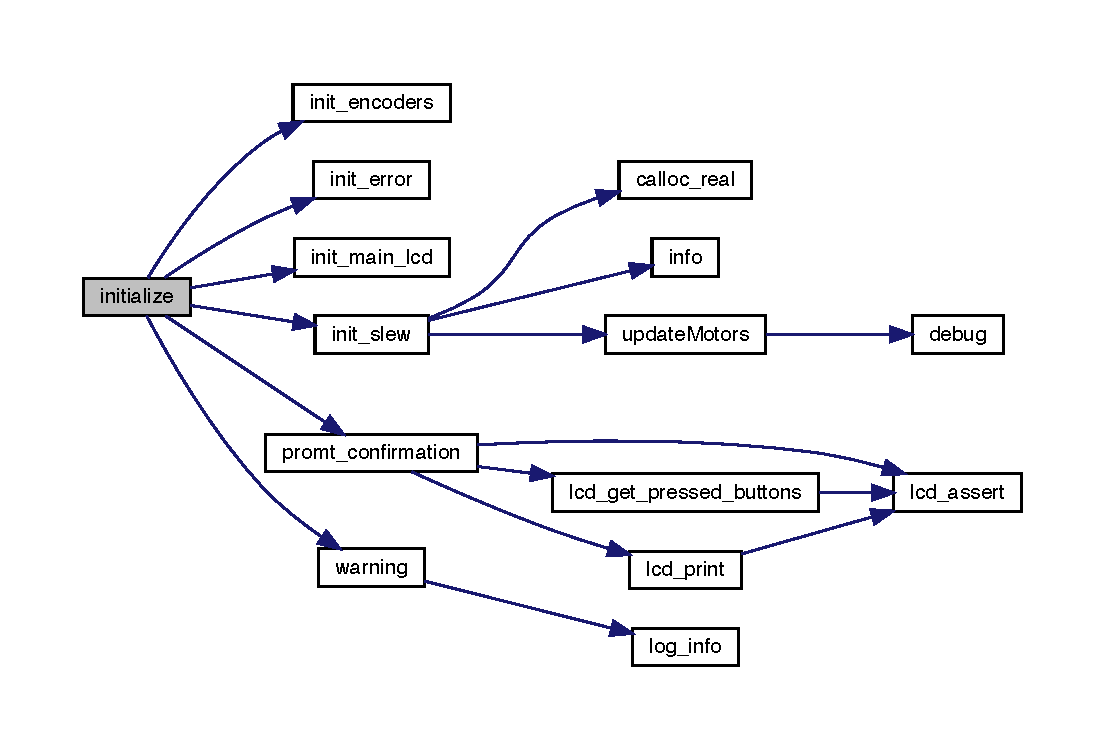
\includegraphics[width=350pt]{init_8c_a25a40b6614565f755233080a384c35f1_cgraph}
\end{center}
\end{figure}
\mbox{\label{init_8c_ad9cda921edb01125bb13c2f86bcf624b}} 
\index{init.\+c@{init.\+c}!initialize\+IO@{initialize\+IO}}
\index{initialize\+IO@{initialize\+IO}!init.\+c@{init.\+c}}
\paragraph{initialize\+I\+O()}
{\footnotesize\ttfamily void initialize\+IO (\begin{DoxyParamCaption}{ }\end{DoxyParamCaption})}



Runs pre-\/initialization code. 

This function will be started in kernel mode one time while the V\+EX Cortex is starting up. As the scheduler is still paused, most A\+PI functions will fail.

The purpose of this function is solely to set the default pin modes (\doxyref{pin\+Mode()}{p.}{_a_p_i_8h_a1875409d12eee562555bda94cad7f973}) and port states (\doxyref{digital\+Write()}{p.}{_a_p_i_8h_a23e767e5b47fa61d4e2cc02e6f15c7ab}) of limit switches, push buttons, and solenoids. It can also safely configure a U\+A\+RT port (usart\+Open()) but cannot set up an L\+CD (\doxyref{lcd\+Init()}{p.}{_a_p_i_8h_a43dc11a67b697c0d32315ea5a9af85f9}). 

Definition at line \textbf{ 36} of file \textbf{ init.\+c}.



References \textbf{ watchdog\+Init()}.


\begin{DoxyCode}
00036 \{ watchdogInit(); \}
\end{DoxyCode}
Here is the call graph for this function\+:
\nopagebreak
\begin{figure}[H]
\begin{center}
\leavevmode
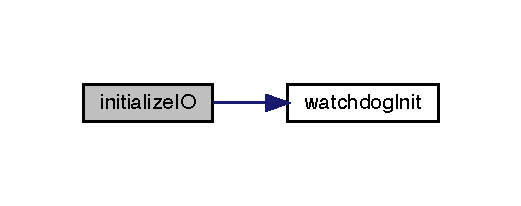
\includegraphics[width=250pt]{init_8c_ad9cda921edb01125bb13c2f86bcf624b_cgraph}
\end{center}
\end{figure}


\subsubsection{Variable Documentation}
\mbox{\label{init_8c_a5dfaf05eb7e97b2e29d04eb068f9c240}} 
\index{init.\+c@{init.\+c}!lifter\+\_\+ultrasonic@{lifter\+\_\+ultrasonic}}
\index{lifter\+\_\+ultrasonic@{lifter\+\_\+ultrasonic}!init.\+c@{init.\+c}}
\paragraph{lifter\+\_\+ultrasonic}
{\footnotesize\ttfamily \textbf{ Ultrasonic} lifter\+\_\+ultrasonic}



Definition at line \textbf{ 24} of file \textbf{ sensors.\+h}.



Referenced by \textbf{ autostack\+\_\+routine()}, \textbf{ initialize()}, and \textbf{ main\+\_\+lifter\+\_\+update()}.


\hypertarget{opcontrol_8c}{}\section{src/opcontrol.c File Reference}
\label{opcontrol_8c}\index{src/opcontrol.\+c@{src/opcontrol.\+c}}


File for operator control code.  


{\ttfamily \#include \char`\"{}main.\+h\char`\"{}}\newline
{\ttfamily \#include \char`\"{}slew.\+h\char`\"{}}\newline
{\ttfamily \#include \char`\"{}drive.\+h\char`\"{}}\newline
{\ttfamily \#include \char`\"{}lifter.\+h\char`\"{}}\newline
{\ttfamily \#include \char`\"{}localization.\+h\char`\"{}}\newline
{\ttfamily \#include \char`\"{}claw.\+h\char`\"{}}\newline
{\ttfamily \#include \char`\"{}mobile\+\_\+goal\+\_\+intake.\+h\char`\"{}}\newline
{\ttfamily \#include \char`\"{}vmath.\+h\char`\"{}}\newline
Include dependency graph for opcontrol.\+c\+:
\nopagebreak
\begin{figure}[H]
\begin{center}
\leavevmode
\includegraphics[width=350pt]{opcontrol_8c__incl}
\end{center}
\end{figure}
\subsection*{Functions}
\begin{DoxyCompactItemize}
\item 
void \hyperlink{opcontrol_8c_ac71a94af413917f27d108e95c4d6f6a7}{operator\+Control} ()
\end{DoxyCompactItemize}


\subsection{Detailed Description}
File for operator control code. 

This file should contain the user \hyperlink{opcontrol_8c_ac71a94af413917f27d108e95c4d6f6a7}{operator\+Control()} function and any functions related to it.

Any copyright is dedicated to the Public Domain. \href{http://creativecommons.org/publicdomain/zero/1.0/}{\tt http\+://creativecommons.\+org/publicdomain/zero/1.\+0/}

P\+R\+OS contains Free\+R\+T\+OS (\href{http://www.freertos.org}{\tt http\+://www.\+freertos.\+org}) whose source code may be obtained from \href{http://sourceforge.net/projects/freertos/files/}{\tt http\+://sourceforge.\+net/projects/freertos/files/} or on request. 

\subsection{Function Documentation}
\mbox{\Hypertarget{opcontrol_8c_ac71a94af413917f27d108e95c4d6f6a7}\label{opcontrol_8c_ac71a94af413917f27d108e95c4d6f6a7}} 
\index{opcontrol.\+c@{opcontrol.\+c}!operator\+Control@{operator\+Control}}
\index{operator\+Control@{operator\+Control}!opcontrol.\+c@{opcontrol.\+c}}
\subsubsection{\texorpdfstring{operator\+Control()}{operatorControl()}}
{\footnotesize\ttfamily void operator\+Control (\begin{DoxyParamCaption}{ }\end{DoxyParamCaption})}

Runs the user operator control code. This function will be started in its own task with the default priority and stack size whenever the robot is enabled via the Field Management System or the V\+EX Competition Switch in the operator control mode. If the robot is disabled or communications is lost, the operator control task will be stopped by the kernel. Re-\/enabling the robot will restart the task, not resume it from where it left off.

If no V\+EX Competition Switch or Field Management system is plugged in, the V\+EX Cortex will run the operator control task. Be warned that this will also occur if the V\+EX Cortex is tethered directly to a computer via the U\+SB A to A cable without any V\+EX Joystick attached.

Code running in this task can take almost any action, as the V\+EX Joystick is available and the scheduler is operational. However, proper use of \hyperlink{_a_p_i_8h_a1c59207742a1acf45a8957d7f04f9dfe}{delay()} or \hyperlink{_a_p_i_8h_ae93bc867b1aa4a12d6536a497f1b6869}{task\+Delay\+Until()} is highly recommended to give other tasks (including system tasks such as updating L\+C\+Ds) time to run.

This task should never exit; it should end with some kind of infinite loop, even if empty. 

Definition at line 40 of file opcontrol.\+c.



References delay(), init\+\_\+slew(), update\+\_\+claw(), update\+\_\+control(), update\+\_\+drive\+\_\+motors(), update\+\_\+lifter(), and update\+Intake().


\begin{DoxyCode}
40                        \{
41     \hyperlink{slew_8h_a321758941d88b75783955c819bb75005}{init\_slew}();
42     \hyperlink{_a_p_i_8h_a1c59207742a1acf45a8957d7f04f9dfe}{delay}(10);
43     \textcolor{keywordflow}{while} (1) \{
44         \hyperlink{drive_8h_a8224a4626a934d30ed587671b7004bf8}{update\_drive\_motors}();
45         \hyperlink{lifter_8h_a59bb7413777ca16aba124aaedf95c79b}{update\_lifter}();
46         \hyperlink{claw_8h_a0122b78972344264b8a276a559cfce4a}{update\_claw}();
47         \hyperlink{mobile__goal__intake_8h_ad0232c21c5c1ffda603d2b7d61034118}{updateIntake}();
48         \hyperlink{partner_8h_ab2c78903a76d2ed8969271803c78368a}{update\_control}();
49         \hyperlink{_a_p_i_8h_a1c59207742a1acf45a8957d7f04f9dfe}{delay}(25);
50     \}
51 \}
\end{DoxyCode}
Here is the call graph for this function\+:\nopagebreak
\begin{figure}[H]
\begin{center}
\leavevmode
\includegraphics[width=350pt]{opcontrol_8c_ac71a94af413917f27d108e95c4d6f6a7_cgraph}
\end{center}
\end{figure}

%--- End generated contents ---

% Index
\backmatter
\newpage
\phantomsection
\clearemptydoublepage
\addcontentsline{toc}{chapter}{Index}
\printindex

\end{document}
